
\documentclass[]{article}

\usepackage{graphicx}
\usepackage[margin=1.5cm,top=1.5cm,bottom=1.5cm,a4paper]{geometry}
\usepackage{graphicx} % Required for inserting images
\usepackage{titlesec} % Required for customizing section titles
\usepackage[margin=1.5cm,top=1.5cm, bottom=1.5cm]{geometry} % Ajusta los márgenes aquí
\usepackage{multicol} % Required for multicols environment
\usepackage{parskip}
\usepackage{etoolbox}
\usepackage{tcolorbox}
\usepackage{float}
\usepackage{amsmath}
\usepackage{dingbat}
\usepackage{booktabs} 
\usepackage{caption}
\usepackage[utf8]{inputenc}
\usepackage[T1]{fontenc}
\usepackage{amssymb}
\usepackage[spanish]{babel}
\usepackage{multirow}
\usepackage{siunitx}
\usepackage{circuitikz}
\usepackage{pdflscape}
\usepackage{subcaption}
\usepackage{array}
\usepackage{tcolorbox}
\usepackage{xcolor}
\usepackage{pdfpages}
\usepackage{placeins}

\newif\ifcheckpoint
\checkpointtrue

% función que devuelve color según checkpoint
\newcommand{\checkpointcolor}[1]{%
	\ifcase#1
	yellow%
	\or blue%
	\or green%
	\or red%
	\or orange%
	\else gray%
	\fi
}
\newcommand{\checkpointstart}[1]{%
	\ifcheckpoint
	\edef\tempcolor{\checkpointcolor{#1}}%
	\begin{tcolorbox}[
		colback=\tempcolor!15,
		colframe=\tempcolor!60!black,
		boxrule=0pt,
		arc=0pt,
		width=\textwidth
		]
		\textbf{Inicio checkpoint #1}
	\end{tcolorbox}
	\fi
}

\newcommand{\checkpointend}[1]{%
	\ifcheckpoint
	\edef\tempcolor{\checkpointcolor{#1}}%
	\begin{tcolorbox}[
		colback=\tempcolor!15,
		colframe=\tempcolor!60!black,
		boxrule=0pt,
		arc=0pt,
		width=\textwidth
		]
		\textbf{Fin checkpoint #1}
	\end{tcolorbox}
	\fi
}

\usepackage{tikz}
\usetikzlibrary{arrows.meta, positioning}
\usetikzlibrary{babel}

\usepackage{csquotes}

\usepackage[
backend=biber,
style=apa,
citestyle=apa
]{biblatex}

\addbibresource{referencias.bib}


\begin{document}
	
	\begin{titlepage}
		
		\centering
		{
\includegraphics[scale=0.5]{img/Caratula.jpg}}
		
		\centerline
		
		{\bfseries\LARGE Taller de Diseño de Circuitos Electrónicos   \par}
		
		{\bfseries\LARGE TA138  \par}
		\vspace{.5cm}
		{\scshape\Large Facultad de Ingenier\'ia Universidad de Buenos Aires \par}
		\vspace{1.5cm}
		%{\scshape\Huge Trabajo Pr\'actico \par}
		{\scshape\Huge Diseño de Fuente de Alimentación \par}
		\vspace{2cm}
		{\scshape\Large MEMORIA TÉCNICA \par}
		
		
		\vspace{2cm}
		
		\begin{tabular}{ p{4cm} p{2cm} p{4cm}}
			\textbf{Alumnos:} & \textbf{Padr\'on:} & \textbf{Mail:} \\
			Lazo, Sebastian Nahuel & 106213 &slazo@fi.uba.ar \\
			Flores, Ahmed Ali & 106238 & aaflores@fi.uba.ar  \\
			Mántaras, Ramiro  & 111510 &rmantaras@fi.uba.ar \\
			
		\end{tabular}
		
		
		\vspace{1cm}
		
		\begin{tabular}{ p{6cm} p{6cm} p{6cm}}
			\textbf{Docentes:}  
			\\Teóricas: Julio Zola & Tutor: Sergio Andres Quinteros  
		\end{tabular}\par
		\vspace{2cm}
		{\scshape\Large 1er cuatrimestre 2026}
		
	\end{titlepage}
	
	
	\newpage
	
	
	\tableofcontents \label{Indice}
	\newpage
	
	\section{Objetivo}

	
	Se propone el diseño, validación e implementación de un sistema electrónico capaz de generar una tensión regulada de 5 V a partir de una fuente de alimentación proveniente de una batería cuya tensión puede variar en un amplio rango comprendido entre 12 V y 30 V. Además de garantizar una salida estable, el sistema debe ser energéticamente eficiente, ya que en aplicaciones reales la eficiencia de conversión es un aspecto fundamental para reducir pérdidas de potencia, calentamiento y consumo energético.
	
	
	El diseño resultante tiene como objetivo combinar alta eficiencia energética, estabilidad de la tensión de salida y confiabilidad operativa, características fundamentales en sistemas de alimentación destinados a cargas como
	microprocesadores, sensores y transceptores de comunicación, tanto para aplicaciones automotrices como industriales.
	
	En total, el dispositivo debe contar con las siguientes especificaciones:
	
	\begin{table}[h]
		\centering
		\renewcommand{\arraystretch}{1.5}
		\begin{tabular}{|p{3cm}|l|l|c|c|c|c|}
			\hline
			\textbf{Característica} & \textbf{Símbolo} & \textbf{Condiciones de prueba} & \textbf{Min.} & \textbf{Tip.} & \textbf{Max.} & \textbf{Unidades} \\
			\hline
			
			\multicolumn{7}{|l|}{\textbf{Especificaciones Generales}} \\
			\hline
			
			Rango de operación tensión de entrada & VIN &  & 12 & 24 & 30 & V \\
			\hline
			
		%	VIN UVLO \par arranque & VIN\_UVLO\_START & VIN creciendo &  &  &  & V \\
		%	\hline
			
		%	VIN UVLO \par apagado & VIN\_UVLO\_STOP & VIN decreciendo &  &  &  & V \\
		%	\hline
			
		%	VIN UVLO \par histéresis & VIN\_UVLO\_HYST &  &  &  &  & V \\
		%	\hline
			
		%	\multirow{2}{3cm}{Corriente de alimentación inactivo} & IQ & VIN=12V &  &  &  & mA \\
		%	\cline{2-7}
		%	& IQ\_Sleep & ENABLE=0 &  &  &  & mA \\
		%	\hline
		\end{tabular}
		\caption{Especificaciones Generales.}
	\end{table}
	
	\section{Diseño y elección de componentes}
	
	La construcción del dispositivo se divide en dos secciones: 
	\begin{itemize}
		\item \textbf{Fuente Switching}: Encargada de pre-regular la tensión de forma eficiente desde la fuente de energía hacia el regulador lineal.
		\item \textbf{Regulador Lineal}: Sacrifica eficiencia a cambio de precisión y control. Interactúa de forma directa con la carga.
	\end{itemize}
	
	\begin{figure}[h]
		\centering
		
\includegraphics[width=0.85\linewidth]{img/esquema_general}
		\caption{Esquema general del dispositivo.}
		\label{fig:esquemageneral}
	\end{figure}

	\subsection{Fuente de alimentación conmutada}
	
	La fuente conmutada será la primera línea de entrada. Predece al regulador lineal, y su objetivo es operar con altas ganancias, realizando el trabajo pesado de reducción de tensión a la salida, para aligerar al regulador lineal. Esto mejora enormemente la eficiencia general del sistema.
	
	\subsubsection{Especificaciones}
	
	Las especificaciones que se busca obtener para esta etapa son las siguientes:
	
		\begin{table}[H]
		\centering
		\renewcommand{\arraystretch}{1.5}
		\begin{tabular}{|p{3cm}|l|p{5cm}|c|c|c|c|}
			\hline
			\textbf{Característica} & \textbf{Símbolo} & \textbf{Condiciones de prueba} & \textbf{Min.} & \textbf{Tip.} & \textbf{Max.} & \textbf{Unidades} \\
			\hline
			
			\multicolumn{7}{|l|}{\textbf{Especificaciones regulador \textit{BUCK}}} \\
			\hline
			
			Eficiencia & $\eta$ & $\SI{12}{V} < V_{IN} < \SI{30}{V}$ \break $\SI{750}{mA} < I_{out} < \SI{1.5}{A}$ & 85 & 90 & 95 & \% \\
			\hline
			
			Frecuencia de conmutación & $f_{sw}$ &  & 120 &  & 140 & \si{\kilo\hertz} \\
			\hline
			
			Tensión regulada & $VREG$ & $\SI{12}{V} < V_{IN} < \SI{30}{V}$ \break $\SI{100}{mA} < I_o < \SI{1.5}{A}$ \break $f_{sw} = \SI{120}{\kilo\hertz}$ & 9,3 & 9,5  & 9,7 & \si{V} \\
			\hline
		\end{tabular}
		
		\caption{Especificaciones del regulador lineal LDO.}
		\label{tab:especificaciones_buck}
	\end{table}
	
	\subsubsection{implementación}
	
	La implementación se hará mediante un a fuente tipo \textit{Buck} síncrona realimentada. Se utilizan dos N-MOS a modo de llave, ya que suelen tener una mejor eficiencia que los transistores P-MOS. Por este motivo, se incorpora un gate driver capaz de generar una sobretensión para el nodo de control del transistor de paso $Q_1$ (figura \ref{fig:bloques_buck}).
	
	\begin{figure}[H]
		\centering
		\begin{tikzpicture}[transform shape]
			% Paths, nodes and wires:
			\node[shape=rectangle, draw, line width=1pt, minimum width=2.215cm, minimum height=1.777cm](N1) at (18.375, 11.906){} node[anchor=south] at ([yshift=-0.12cm]N1.text){$Gate \ Driver$};
			\draw (17.25, 11.813) -- (16, 11.813);
			\draw (17.25, 11.312) -- (16.75, 11.312) -| (16.75, 11.063);
			\node[tlground] at (16.75, 11.063){};
			\node[trarrow, xscale=-1, yscale=-1](N2) at (16.112, 9){} node[anchor=south] at (N2.text){$PWM$};
			\draw (15.888, 12.563) -- (17.25, 12.563);
			\node[trarrow](N3) at (15.888, 12.563){} node[anchor=east] at (N3.text){$V_{cc12}$};
			\node[nigfetd, rotate=90](N4) at (17.77, 16.29){} node[anchor=south] at (N4.text){$Q_1$};
			\node[nigfetd](N5) at (20, 14.56){} node[anchor=west] at (N5.text){$Q_2$};
			\draw (24, 16.29) to[capacitor, l={$C_S$}] (24, 13.29);
			\draw (26, 16.29) to[american resistor, l={$R_S$}] (26, 13.29);
			\draw (20, 16.29) -- (20, 15.29);
			\draw (24, 13.29) |- (20, 13.29) -| (20, 13.75);
			\draw (24, 16.29) -- (26, 16.29);
			\draw (26, 13.29) -- (24, 13.29);
			\draw (20, 13.79) -| (20, 13.75);
			\draw (15, 13.29) to[capacitor, l={$C_E$}] (15, 16.29);
			\draw (15, 13.29) -- (20, 13.29);
			\draw (15, 16.29) -- (17, 16.29);
			\draw (18.54, 16.29) -- (20, 16.29);
			\draw (20, 16.29) to[cute inductor, l={$L$}] (24, 16.29);
			\draw (12, 16.29) to[battery, l={$V_E$}] (12, 13.29);
			\node[circ] at (15, 16.29){};
			\node[circ] at (15, 13.29){};
			\node[circ] at (20, 13.29){};
			\node[circ](N6) at (20, 16.29){} node[anchor=south] at (N6.text){$V_S$};
			\node[circ] at (24, 16.29){};
			\node[circ] at (24, 13.29){};
			\node[circ](N7) at (26, 16.29){} node[anchor=south] at (N7.text){$V_o$};
			\draw (26, 16.29) -- (27, 16.29);
			\draw (15, 16.29) -- (12, 16.29);
			\draw (15, 13.29) |- (12, 13.29);
			\node[shape=rectangle, draw, line width=1pt, minimum width=1.965cm, minimum height=1.777cm] at (12, 10.5){};
			\draw (12, 9.594) to[empty Schottky diode, /tikz/circuitikz/bipoles/length=0.980cm] (12, 11.406);
			\node[shape=rectangle, draw, line width=1pt, minimum width=1.965cm, minimum height=1.027cm](N8) at (19.75, 8.5){} node[anchor=north] at ([yshift=-0.49cm]N8.text){$Triangular$};
			\node[circ](N9) at (12, 11.906){} node[anchor=south] at (N9.text){$V_E$};
			\draw (12, 11.906) -- (12, 11.406);
			\node[tlground] at (12, 9.156){};
			\draw (12, 9.156) -| (12, 9.594);
			\draw (13, 10.906) -- (13.5, 10.906);
			\node[trarrow](N10) at (13.5, 10.906){} node[anchor=west] at (N10.text){$V_{cc12}$};
			\draw (13, 10.156) -- (13.5, 10.156);
			\node[trarrow](N11) at (13.5, 10.156){} node[anchor=west] at (N11.text){$V_{cc2}$};
			\draw (28, 12) to[american resistor, /tikz/circuitikz/bipoles/length=0.980cm, l={$R_1$}] (28, 10);
			\draw (28, 10) to[american resistor, /tikz/circuitikz/bipoles/length=0.980cm, l={$R_2$}] (28, 8);
			\node[tlground] at (28, 8){};
			\draw (27, 16.29) -| (28, 12);
			\draw (18.04, 15.31) |- (17.875, 12.813);
			\draw (19.02, 14.29) |- (18.375, 12.813);
			\draw (20, 16.29) -- (18.5, 14.75);
			\draw (18.5, 14.75) |- (18.375, 12.813);
			\node[op amp, xscale=-1, yscale=-1] at (17.31, 9.01){};
			\node[op amp, xscale=-1] at (21.81, 9.49){};
			\node[currarrow, xscale=-1, yscale=-1](N12) at (23, 9){} node[anchor=west] at (N12.text){$Vcc_{12}/2$};
			\draw (28, 10) |- (23, 9.98);
			\node[circ] at (28, 9.98){};
			\draw (18.5, 9.5) -| (20.62, 9.49);
			\draw (18.5, 8.52) -| (18.75, 8.5);
			\draw (19, 8.25) -- (19.25, 8.75) -- (19.5, 8.25) -- (19.75, 8.75) -- (20, 8.25) -- (20.25, 8.75) -- (20.5, 8.25);
			\draw (16.12, 9.02) |- (15, 9.01) -| (15, 11.76) |- (16, 11.823);
			\draw (20.5, 9.5) to[empty Schottky diode, /tikz/circuitikz/bipoles/length=0.980cm] (20.5, 10.75);
			\node[circ](N13) at (20.5, 10.75){} node[anchor=south] at (N13.text){$Vcc2$};
			\node[circ] at (20.5, 9.5){};
		\end{tikzpicture}
		\caption{Circuito simplificado de la fuente \textit{Buck}.}
		\label{fig:bloques_buck}
	\end{figure}
	
	El lazo de realimentación consta de un amplificador de error, cuya función es producir la diferencia entre la señal objetivo ($Vcc_{12}/2$) y la señal muestreada mediante el divisor resisitivo $R_1$ - $R_2$. Esta señal se compara con otra señal, perdiódica con forma triangular, para convertirla en una señal tipo PWM, que se encarga de controlar los transistores de paso.
	
	
	\subsubsection{Convertidor BUCK a lazo abierto}
	
	En términos generales, un convertidor \textit{buck} se alimenta de una señal de entrada a a regular, por medio de dos transistores en conmutación, que generan una señal cuadrada que tiene como valor medio la tensión objetivo, la señal cuadrada generada es filtrada por un filtro LC, obteniendo de esta forma una tensión regulada con riple cuadrático. En la figura \ref{fig:buck_schematic}, se observa un circuito \textit{buck} inicial de diseño.
	
	\begin{figure}[H]
		\centering
		\resizebox{0.9\textwidth}{!}{
			\begin{tikzpicture}[transform shape]
				% Paths, nodes and wires:
				\node[nigfetd, rotate=90](N1) at (11.77, 11){} node[anchor=south] at (N1.text){$Q_1$};
				\node[nigfetd](N2) at (14, 9.27){} node[anchor=west] at (N2.text){$Q_2$};
				\draw (18, 11) to[capacitor, l={$C_S$}] (18, 8);
				\draw (20, 11) to[american resistor, l={$R_S$}] (20, 8);
				\draw (14, 11) -- (14, 10);
				\draw (18, 8) |- (14, 8) -| (14, 8.46);
				\draw (18, 11) -- (20, 11);
				\draw (20, 8) -- (18, 8);
				\draw (12.039, 10.02) |- (11, 9.5);
				\draw (14, 8.5) -| (14, 8.46);
				\draw (13.02, 9) -| (11, 9);
				\draw (9, 8) to[capacitor, l={$C_E$}] (9, 11);
				\draw (9, 8) -- (14, 8);
				\draw (9, 11) -- (11, 11);
				\draw (12.54, 11) -- (14, 11);
				\draw (14, 11) to[cute inductor, l={$L$}] (18, 11);
				\draw (6, 11) to[battery, l={$V_E$}] (6, 8);
				\node[circ] at (9, 11){};
				\node[circ] at (9, 8){};
				\node[circ](N3) at (11, 9.5){} node[anchor=east] at (N3.text){$H_{ctrl}$};
				\node[circ](N4) at (11, 9){} node[anchor=east] at (N4.text){$L_{ctrl}$};
				\node[circ] at (14, 8){};
				\node[circ](N5) at (14, 11){} node[anchor=south] at (N5.text){$V_S$};
				\node[circ] at (18, 11){};
				\node[circ] at (18, 8){};
				\node[circ](N6) at (20, 11){} node[anchor=south] at (N6.text){$V_o$};
				\node[flowarrow] at (21.25, 11){};
				\draw (20, 11) -- (21, 11);
				\draw (9, 11) -- (6, 11);
				\draw (9, 8) |- (6, 8);
			\end{tikzpicture}
		}
		\caption{Circuito \textit{buck}.}
		\label{fig:buck_schematic}
		
	\end{figure}
	
	Entendiendo la señal de control como una señal periódica cuadrada que alterna entre una tensión suficiente para colocar a los transistores en saturación (\textit{on}) y otra que los lleva a corte (\textit{off}), en dicha señal se define el tiempo $t_{ON}$ como el tiempo que dura la señal que permite la conducción en el transistor en un periodo T. Aquí a su vez se define el ciclo de trabajo D (duty cicle) como $ D = \frac{t_{ON}}{T}$. 
	
	\begin{figure}[H]
		\centering
		
\includegraphics[width=1\linewidth]{img/buck/vcontrol}
		\caption{ Señal de control y señal conmutada lograda en el circuito buck.}
		\label{fig:vcontrol}
	\end{figure}
	
	Teniendo en cuenta que el transistor permite replicar la señal de control en el nodo que interconecta los transistores y el inductor, pero con una tensión cercana a la tensión de alimentación, dicha señal se define como señal de conmutación o \textit{switching} $V_s$. Tal como se ve en la figura \ref{fig:vcontrol}.
	
	
	De esta relación estimando las tensiones de saturación y de caida de tensión en directa del diodo utilizado, se puede dar con una primer aproximación de D. Aproximando la salida del regulador como la componente continua de la señal de conmutación, idealizando el filtro LC.
	
	
	\begin{equation}
		V_o \approx V_{s_{\text{prom}}}
		=
		\frac{1}{T}\int_0^T v_s(t)\,dt
	\end{equation}
	
	Considerando que durante el intervalo de conducción del transistor ($t_{on}$) la tensión aplicada al inductor es aproximadamente $(V_E - V_{SAT})$, y durante el intervalo restante ($T-t_{on}$) el diodo conduce imponiendo una tensión aproximada $-V_D$, la señal de conmutación puede modelarse como:
	
	\begin{equation}
		v_s(t)=
		\begin{cases}
			V_E - V_{SAT}, & 0<t<t_{on} \\
			-V_{SAT}, & t_{on}<t<T
		\end{cases}
	\end{equation}
	
	Por lo tanto, el valor promedio resulta:
	
	\begin{equation}
		V_o \approx
		\frac{1}{T}
		\left[
		\int_0^{t_{on}} (V_E - V_{SAT})\,dt
		+
		\int_{t_{on}}^T (-V_{SAT})\,dt
		\right]
	\end{equation}
	
	Resolviendo las integrales:
	
	\begin{equation}
		V_o \approx
		\frac{1}{T}
		\left[
		(V_E - V_{SAT})t_{on}
		-
		V_{SAT}(T-t_{on})
		\right]
	\end{equation}
	
	Reordenando:
	
	\begin{equation}
		V_o \approx
		\frac{t_{on}}{T}(V_E - V_{SAT})
		-
		\frac{T-t_{on}}{T}V_{SAT}
	\end{equation}
	
	Definiendo el ciclo de trabajo como:
	
	\begin{equation}
		D = \frac{t_{on}}{T}
	\end{equation}
	
	y teniendo en cuenta que:
	
	\begin{equation}
		1-D = \frac{T-t_{on}}{T}
	\end{equation}
	
	se obtiene finalmente:
	
	\begin{equation}
		V_o \approx D(V_E - V_{SAT}) - (1-D)V_{SAT}
	\end{equation}
	
	
	Aproximando las caídas de tensión de los transistores en conducción a cero:
	
	\begin{equation}
		V_{SAT} \approx 0
	\end{equation}
	
	la expresión obtenida previamente se simplifica a:
	
	\begin{equation}
		V_o \approx D \cdot V_E
	\end{equation}
	
	Despejando el ciclo de trabajo:
	
	\begin{equation}
		D \approx \frac{V_o}{V_E}
	\end{equation}
	
	Reemplazando con los valores de diseño:
	
	\begin{equation}
		D \approx \frac{9.5\,V}{24\,V}
	\end{equation}
	
	\begin{equation}
		D \approx 0.396
	\end{equation}
	
	Por lo tanto, el ciclo de trabajo requerido resulta aproximadamente:
	
	\begin{equation}
		D \approx 39.6\%
	\end{equation}
	
	
	El principio de funcionamiento del regulador se basa en la transferencia periódica de energía desde la fuente de entrada hacia la carga mediante la conmutación controlada de los dispositivos electrónicos de potencia. La tensión media de salida se regula variando el ciclo de trabajo $D$ de la señal PWM aplicada a las llaves de conmutación.
	
	
	Asimismo, se analizará el regulador operando en modo de conducción continua (CCM, \textit{Continuous Conduction Mode}), condición en la cual la corriente del inductor nunca se anula ni invierte su sentido. Bajo esta hipótesis, la corriente del inductor presenta una forma aproximadamente triangular con un valor medio distinto de cero, mientras que el capacitor forma una tensión integrando dicha tensión menos la corriente de salida, dado que la integral de una señal lineal que alterna entre pendiente positiva y negativa la tensión del capacitor sera una señal cuadrática tal como se observa en la figura \ref{fig:corrienteilriplevo}.
	
	A partir de estas consideraciones será posible determinar posteriormente los valores adecuados del inductor $L$ y del capacitor $C$, de forma tal de garantizar un funcionamiento estable en conducción continua y un rizado acotado en corriente y tensión.
	
	
	\begin{figure}[H]
		\centering
		
\includegraphics[width=0.7\linewidth]{img/buck/corriente_iL_riple_Vo}
		\caption{Forma de la señal de corriente en el inductor y tensión en el capacitor del regulador.}
		\label{fig:corrienteilriplevo}
	\end{figure}
	
	La corriente de salida se puede aproximar a la corriente media en el inductor, justamente para que la corriente no se vuelva discontinua la corriente de salida debe ser mayor a cero, es por eso que se fija un resistor de salida para que la corriente de salida no llegue a ser nula. 
	
	\begin{equation}
		I_O \approx \frac{I_{L\text{MAX}} + I_{L\text{MIN}}}{2}
	\end{equation}
	
	
	\subsubsection{Inductor $L$ y capacitor $C_S$}
	
	Teniendo en cuenta que para el ciclo \textit{off} la tensión de salida corresponde con aproximadamente la tensión en el inductor:
	
	\begin{equation}
		V_o \approx L \frac{d i_L }{dt} = L \frac{ {I_{min}} - {I_{max}} }{  T - t_{on}}
	\end{equation} 
	
	Despejando el valor de inductancia:
	
	\begin{equation}
		L \approx V_o  \frac{  T - t_{on}}{ {I_{min}} - {I_{max}} }
	\end{equation} 
	
	Sacando como factor común T de la expresión e ingresando D.
	
	\begin{equation}
		L \approx V_o  \frac{  T - t_{on}}{ {I_{min}} - {I_{max}} } =  V_o  T \frac{  (1 - \frac{t_{on}}{T})}{ {I_{min}} - {I_{max}} } 
	\end{equation} 
	
	
	\begin{equation}
		L \approx  V_o  T \frac{  1 - D} {   I_{min} - {I_{max}}    } 
	\end{equation} 
	
	Ahora sabiendo que $I_o = \frac{(I_{min} - I_{max})}{2}$ y despejando $ I_{min} = 2I_o - I_{max}$, se reemplaza:
	
	\begin{equation}
		L \approx  V_o \cdot T \frac{  1 - D} {   (2I_o - I_{max}) - {I_{max}}    } 
	\end{equation} 
	
	
	\begin{equation}
		L \approx  V_o \cdot T \frac{  1 - D} {   (2I_o - 2I_{max})   }  = V_o \cdot T \frac{  1 - D} {   2(I_o - I_{max})   }
	\end{equation} 
	
	
	
	\begin{equation}
		L \approx  V_o \cdot T \frac{  1 - D} {   (2I_o - 2I_{max})   }  = V_o  \frac{T}{2} \frac{  1 - D} {   (I_o - I_{max})   }
	\end{equation} 
	
	Reemplazando $T = \frac{1}{f}$ se obtiene finalmente la expresión:
	
	\begin{equation}
		L =
		\frac{1}{2f}
		\left(
		\frac{(1-D)V_S}{I_{L\text{MAX}} - I_o}
		\right)
	\end{equation}
	
	De esta forma se puede estimar un valor de inductancia 
	Partiendo de:
	
	\begin{equation}
		L = \frac{1}{2f}\,\frac{(1-D)V_o}{(I_{L\text{MAX}} - I_o)}
	\end{equation}
	
	y siendo para el modo crítico:
	
	\begin{equation}
		I_o = I_{o\text{MIN}}
	\end{equation}
	
	Resulta:
	
	\begin{equation}
		I_{L\text{MAX}} = 2I_{o\text{MIN}}
	\end{equation}
	
	\begin{equation}
		L = \frac{(1-D)V_o}{2f\,I_{o\text{MIN}}}
	\end{equation}
	
	Llamando \(R_{\text{MAX}}\) al valor máximo de \(R_c\):
	
	\begin{equation}
		R_{\text{MAX}} = \frac{V_o}{I_{o\text{MIN}}}
	\end{equation}
	
	se obtiene el valor crítico de \(L\) (\(L_{cr}\)) que permite continuar operando en modo continuo con una corriente de carga mínima o “carga mínima”:
	
	\begin{equation}
		L_{cr} = \frac{(1-D)R_{\text{MAX}}}{2f}
	\end{equation}
	
	Debe ser:
	
	\begin{equation}
		L > L_{cr}
	\end{equation}
	
	para operación en modo continuo.
	
	También puede encontrarse el valor crítico de la resistencia de carga que asegura el funcionamiento en modo continuo para un valor dado de \(L\):
	
	\begin{equation}
		R_{cr} = \frac{2fL}{(1-D)}
	\end{equation}
	
	Debe cumplirse:
	
	\begin{equation}
		R < R_{cr}
	\end{equation}
	
	para operación en modo continuo.
	
	Contemplando la frecuencia mayor brindada por las especificación con el objetivo de minimizar el riple en la salida, ya que el filtro pasa bajos LC atenuara mucho mas las frecuencias altas y también nos dará valores de L y C mas bajos para el mismo filtro.
	
	Reemplazando en las expresiones con los valores de frecuencia elegida $f = 140 \, kHz$, ciclo de trabajo $D = 0,395$, $I_{min} = 1.4 \, A$, $I_{max} = 1,6 \,A$ y rimple de $\Delta V_o = 400 \, mV$, llegando a los valores críticos: 
	
	\renewcommand{\arraystretch}{1.5}
	\begin{table}[H]
		\centering
		\caption{Valores críticos para conservar la conducción continua}
		\renewcommand{\arraystretch}{1.5}
		\begin{tabular}{|c|c|c|}
			\hline
			\textbf{Parámetro crítico} & \textbf{Expresión utilizada} & \textbf{Condición para MCC} \\
			\hline
			
			Inductancia crítica \(L_{cr}\) &
			\(
			L_{cr}= \frac{(1-D)V_o}{2f\,I_{o\text{MIN}}}
			\)
			&
			\(
			L > L_{cr} \approx 207 \, \mu H
			\)
			\\
			
			\hline
			
			Resistencia crítica \(R_{cr}\) &
			\(
			R_{cr}=\dfrac{2fL}{(1-D)}
			\)
			&
			\(
			R < R_{cr} \approx 95\, \Omega
			\)
			\\
			
			\hline
			
			Capacitancia crítica \(C_{cr}\) &
			\(
			C_{cr}=\dfrac{1-D}{16Lf^2\left(\dfrac{\Delta V_o}{V_o}\right)}
			\)
			&
			\(
			C > C_{cr} \approx 3,34 \, uF
			\)
			\\
			
			\hline
			
			Corriente mínima de carga \(I_{o\text{MIN}}\) &
			\(
			I_{o\text{MIN}}=\dfrac{(1-D)V_s}{2fL}
			\)
			&
			\(
			I_o >= I_{o\text{MIN}} = 100 \, mA
			\)
			\\
			
			\hline
			
		\end{tabular}
		\label{tab:criticos_mcc}
	\end{table}
	
	
	Con los valores hallados en la tabla \ref{tab:criticos_mcc} se obtienen los limites para que el circuito trabaje en modo conducción continua, pero no serán los valores óptimos para regular la tensión, para asegurar que el riple sea minimo se considera un capacitor $100 \, \mu F$ y para que la corriente continua de salida tenga alguna utilidad se coloca un diodo led que indique que el regulador esta encendido para eso se debe calcular un resistor 
	
	\subsubsection{Transistores de conmutación}
	Para la elección de transistores de paso debe hacerce un balance entre resistencia equivalente en conducción $R_{ON}$, sus capacidades parásitas $C_{gs}$, $C_{gd}$ y $C_{ds}$ y el costo.
	El modelo elegido para la aplicación es el transistor N-MOS \textbf{IRF3205}, debido a su costo moderado
	
	
	\subsubsection{Frecuencia de oscilador}
	
	Como regla práctica, a fin de maximizar la eficiencia, el periodo mínimo del oscilador debe ser aproximadamente cien veces mayor que el tiempo de conmutación del transistor. Porque así el MOSFET pasa más del 99 \% del tiempo en estados ideales (encendido o apagado) y menos del 1 \% del tiempo en la región de transición donde disipa mucha potencia.
	
	
	
	
	
	\begin{minipage}[c]{0.35\textwidth}
		\begin{figure}[H]
			\centering
			
\includegraphics[width= 1\linewidth]{img/buck/tiempo_conmutacionIRF3205}
			\caption{Formas de onda de tiempo de conmutación para el IRF520.}
			\label{fig:tiempoconmutacionirf3205}
		\end{figure}
		
	\end{minipage}
	\hfill
	\begin{minipage}[c]{0.60\textwidth}
		
		\begin{equation}
			T_{sw} = 100\cdot t_{sw}
		\end{equation}
		
		Cuando se aplica la tensión de entrada base, el transistor no se enciende inmediatamente. Al igual que la respuesta de frecuencia, los tiempos de conmutación de transistores se ven afectados por la capacitancia de la unión y el tiempo de tránsito de los electrones a través de las uniones. El tiempo entre la aplicación del impulso de entrada y el comienzo del flujo de corriente del drenaje se denomina el tiempo de retardo (td), incluso cuando el transistor comienza a encenderse, transcurre un tiempo finito antes de que el CI alcance su nivel máximo. Esto se conoce como el tiempo de subida ($t_{d_{on}}$) y de bajada $t_{d_{off}}$.
		
		El tiempo de subida se especifica como el tiempo requerido para que el CI pase del 10\% al 90\% de su nivel máximo. 
		
		
		Para el IRF520 el tiempo de retardo de encendido ($t_{d_{on}}$) es de $15 \, ns$  y el tiempo en que se produce la caída de tensión entre el drain y source es de $t_r = 75 \,ns$ mientras que el tiempo de retardo de apagado ($t_{d_{off}}$) es de $ 40 \, ns$ y el tiempo en que se produce el cambio de tensión en $v_{ds}$ es de $t_f = 30 \, ns $ , por lo tanto se consideran los tiempos de encendidos y de apagado como:
		
		
		\begin{itemize}
			\item $t_{on} =t_{d_{on}} + t_r =  90 \,ns$
			\item $t_{off} = t_{d_{off}} + t_f = 70 \,ns $	
		\end{itemize}
		
		
		Dando asi el tiempo de conmutación como $t_{sw} = 90 \, ns$
		
		
	\end{minipage}
	
	Por lo tanto el periodo de oscilación tiene que ser como mínimo T $ \geq   100 \cdot t_{sw} = 9 \, \mu s$, siendo así la frecuencia máxima para lograr una eficiencia 110 kHz. Por lo tanto al utilizar una frecuencia de 133 kHz se debe considerar una menor eficiencia.
	
	
	
	\begin{table}[H]
		\centering
		\caption{Componentes seleccionados para el convertidor Buck}
		\renewcommand{\arraystretch}{1.5}
		\begin{tabular}{|c|c|c|c|}
			\hline
			\textbf{Componente} & \textbf{Símbolo} & \textbf{Valor / Modelo} & \textbf{Observaciones} \\
			\hline
			
			Inductor de salida & \(L\) & $250 \mu H $&  \\
			\hline
			
			Capacitor de salida & \(C\) & $100 \mu F$ &  \\
			\hline
			
			Capacitor de entrada & \(C_{in}\) & $100 \mu F$ &  \\
			\hline
			
			MOSFET superior & \(Q_1\) & N-MOS IRF520  &  \\
			\hline
			
			MOSFET inferior & \(Q_2\) & N-MOS IRF520  &  \\
			\hline
			
			Frecuencia de conmutación & \(f_s\) & 133 kHz&  \\
			\hline
			
			Tensión de entrada & \(V_{in}\) & 24 V &  \\
			\hline
			
			Tensión de salida & \(V_o\) & 9,5 v  &  \\
			\hline
			
			Corriente máxima de salida & \(I_o\) & 1,5 A &  \\
			\hline
			
		\end{tabular}
		\label{tab:componentes_buck}
	\end{table}
	
	\subsubsection{Diseño del lazo realimentador}
	
	Una vez verificado el diseño de la fuente conmutada, se debe diseñar un lazo capaz de regularla. Para cumplir con este requerimiento, se parte de la salida de la fuente (figura \ref{fig:buck_schematic}), y se genera una señal PWM capaz de controlar la conmutación de los transistores. En la figura \ref{fig:bloque_PWM} puede verse la estructura simplificada del lazo.
	
	
	\begin{figure}[H]
		\centering
		\begin{tikzpicture}[transform shape]
			% Paths, nodes and wires:
			\draw (9.99, 7.5) to[twoport] (11.99, 7.5);
			\draw (10.99, 7.98) to[american resistor, /tikz/circuitikz/bipoles/length=0.700cm] (10.99, 7);
			\node[plain amp, xscale=-1, yscale=-1] at (8.94, 7){};
			\node[circ](N1) at (12, 6.52){} node[anchor=west] at (N1.text){$v_{ref}$};
			\node[circ](N2) at (11.99, 7.49){} node[anchor=west] at (N2.text){$v_{o}$};
			\draw (10, 6.52) -| (12, 6.5);
			\node[nigfetd, xscale=0.5, yscale=0.5] at (4.48, 6.52){};
			\node[plain amp, xscale=-1, yscale=-1] at (6.43, 6.52){};
			\node[shape=rectangle, minimum width=1.465cm, minimum height=0.965cm] at (9, 7){} node[anchor=center, align=center, text width=1.077cm, inner sep=6pt] at (9, 7){\tiny Amplificador de error};
			\node[shape=rectangle, minimum width=1.465cm, minimum height=0.965cm] at (6.5, 6.5){} node[anchor=center, align=center, text width=1.077cm, inner sep=6pt] at (6.5, 6.5){\tiny Comparador PWM};
			\node[shape=rectangle, draw, line width=1pt, minimum width=0.965cm, minimum height=0.965cm] at (4.25, 6.5){};
			\draw (5.24, 6.52) -| (4.75, 6.5);
			\draw (8, 5) |- (7.62, 6.03);
			\draw (8.5, 4.5) |- (8, 4.5) -| (8, 5);
			\node[shape=rectangle, minimum width=1.945cm, minimum height=1.215cm] at (10.01, 4.375){} node[anchor=center, align=center, text width=1.557cm, inner sep=6pt] at (10.01, 4.375){\tiny Generador de señal triangular};
			\node[shape=rectangle, draw, line width=1pt, minimum width=1.945cm, minimum height=1.225cm] at (10.01, 4.38){};
			\draw (9, 4.5) -- (8.5, 4.5);
			\draw (9, 4.5) -| (9.02, 4.51);
			\node[shape=rectangle, minimum width=1.465cm, minimum height=0.965cm] at (11, 8.25){} node[anchor=center, align=center, text width=1.077cm, inner sep=6pt] at (11, 8.25){\small Escalado};
			\node[shape=rectangle, minimum width=1.465cm, minimum height=0.965cm] at (4.25, 7.5){} node[anchor=center, align=center, text width=1.077cm, inner sep=6pt] at (4.25, 7.5){\small Gate Driver};
			\node[shape=rectangle, draw, line width=1pt, minimum width=0.945cm, minimum height=0.965cm] at (4.26, 4.5){};
			\draw (4.26, 4) to[empty Schottky diode, /tikz/circuitikz/bipoles/length=0.840cm] (4.26, 5);
			\draw (4.26, 5) |- (4.25, 5.25);
			\draw (4.26, 4) |- (4.25, 3.75);
			\node[tlground] at (4.25, 3.75){};
			\node[circ](N3) at (4.26, 5.25){} node[anchor=south] at (N3.text){$V_{E}$};
			\draw (4.75, 4.5) -- (5, 4.5);
			\node[circ](N4) at (5, 4.5){} node[anchor=west] at (N4.text){$V_{5V}$};
			\draw (10, 5) |- (9.99, 5.25);
			\draw (10.01, 3.75) |- (10, 3.5);
			\node[tlground] at (10, 3.5){};
			\node[circ](N5) at (10, 5.25){} node[anchor=south] at (N5.text){$V_{5V}$};
			\draw (9, 7.75) |- (8.99, 8);
			\draw (9, 6.5) |- (8.99, 6.25);
			\node[tlground] at (8.99, 6.25){};
			\node[circ](N6) at (9, 8){} node[anchor=south] at (N6.text){$V_{5V}$};
			\draw (9, 7.75) -- (9, 7.5);
			\draw (6.51, 7.25) |- (6.5, 7.5);
			\draw (6.51, 6) |- (6.5, 5.75);
			\node[tlground] at (6.5, 5.75){};
			\node[circ](N7) at (6.51, 7.5){} node[anchor=south] at (N7.text){$V_{5V}$};
			\draw (6.51, 7.25) -- (6.51, 7);
			\draw (7.75, 7) |- (7.62, 7.01);
		\end{tikzpicture}
		\caption{Diagrama de bloques del lazo realimentador.}
		\label{fig:bloque_PWM}
	\end{figure}
	
	Se sensa la señal de salida y se obtiene el error respecto de una referencia. Luego, se compara el error con una señal triangular, cuyo objetivo es aumentar el duty si el error es negativo (tensión de salida baja) y disminuirlo si es positivo.
	
	\subsubsection{Escalador de señal de salida}
	
	Se busca comparar la señal de salida con una tensión de referencia más baja. Para ello debe escalarse $V_o$ de tal modo que, si $V_o$ tiene el valor deseado, $v_{med} = V_o \cdot escalado$. Se elige una combinación de resistores tal que $\SI{9.5}{V} \cdot escalado = v_{med} =\SI{5.75}{V} \to escalado = 0.605$. La figura \ref{fig:escalado} muestra su topología.
	
	\begin{figure}[H]
		\centering
\begin{tikzpicture}[transform shape]
	% Paths, nodes and wires:
	\draw (12, 11) to[american resistor, /tikz/circuitikz/bipoles/length=0.980cm, l={$R_1$}] (12, 9);
	\draw (12, 9) to[american resistor, /tikz/circuitikz/bipoles/length=0.980cm, l={$R_2$}] (12, 7);
	\node[circ] at (12, 9){};
	\node[circ](N1) at (12, 11){} node[anchor=south] at (N1.text){$V_o$};
	\node[tlground] at (12, 7){};
	\node[currarrow, xscale=-1, yscale=-1](N2) at (10.276, 9){} node[anchor=east] at (N2.text){$v_{sense}$};
	\draw (10.25, 9) -- (12, 9);
\end{tikzpicture}
		\caption{Bloque de escalado.}
		\label{fig:escalado}
	\end{figure}
	
	Se eligen dos resistores de valor $R_{1} = \SI{22}{\kilo\ohm}$ y otro de valor $R_2 = \SI{33}{\kilo\ohm}$:
	
	\begin{equation}
		escalado = \frac{R_2}{R_1 + R_2} = 0.6
	\end{equation}
	\subsubsection{Alimentación del lazo y tensión de referencia}
	Para el correcto funcionamiento del lazo, se busca que su tensión de alimentación sea independiente de la entrada $V_{E}$, por dos motivos: para proteger los comparadores y amplificadores de sobretensión, y para reducir el ruido del lazo. Asimismo, y con el objetivo de aumentar al máximo la excursión simétrica, se fija la tensión de referencia en la mitad de la tensión de alimentación.
	
	En la figura \ref{fig:regulador_431} puede verse el circuito de alimentación del lazo realimentador. Se implementa mediante el uso de un regulador ajustable \textbf{TL431} con el agregado de un transistor como fuente de corriente.
	
	Se busca, por limitación de los comparadores y amplificadores elegidos, una tensión de alimentación de \SI{11.5}{V}, y por ende una tensión de referencia de \SI{5.75}{V}
	
	\begin{figure}[H]
		\centering
		\begin{tikzpicture}[transform shape]
			% Paths, nodes and wires:
			\draw (6, 4.75) to[empty Schottky diode, l={$TL431$}] (6, 7.25);
			\draw (6, 8.25) to[american resistor, /tikz/circuitikz/bipoles/length=0.840cm, l={$R_1$}] (6, 9.75);
			\draw (8, 6) to[american resistor, /tikz/circuitikz/bipoles/length=0.840cm, l={$R_2$}] (8, 7.5);
			\draw (8, 4.5) to[american resistor, /tikz/circuitikz/bipoles/length=0.840cm, l={$R_3$}] (8, 6);
			\draw (10, 6) to[american resistor, /tikz/circuitikz/bipoles/length=0.840cm, l={$R_4$}] (10, 7.5);
			\draw (10, 4.5) to[american resistor, /tikz/circuitikz/bipoles/length=0.840cm, l={$R_5$}] (10, 6);
			\node[npn](N1) at (8, 8.27){} node[anchor=west] at (N1.text){$Q_1$};
			\draw (8, 9.04) -| (8, 10) |- (6, 10);
			\draw (6, 9.75) -| (6, 10);
			\draw (6, 8.25) -| (6, 7);
			\draw (7.16, 8.27) -| (6, 8.25);
			\draw (8, 7.5) -- (10, 7.5);
			\draw (10, 4.5) -- (6, 4.5);
			\draw (6, 4.5) -| (6, 4.75);
			\draw (8, 6) |- (6.25, 6);
			\draw (10, 6) -- (11, 6);
			\node[circ] at (6, 8.25){};
			\node[circ] at (8, 6){};
			\node[circ] at (10, 6){};
			\node[circ] at (8, 7.5){};
			\node[circ] at (8, 4.5){};
			\node[rground, xscale=-1, yscale=-1](N2) at (7, 10){} node[anchor=south] at ([yshift=0.32cm]N2.text){$V_E$};
			\node[circ](N3) at (11, 6){} node[anchor=west] at (N3.text){$V_{med}$};
			\draw (10, 7.5) -- (11, 7.5);
			\node[circ] at (10, 7.5){};
			\node[circ](N4) at (11, 7.5){} node[anchor=west] at (N4.text){$V_{5V}$};
			\node[tlground] at (8, 4){};
			\draw (8, 4) -| (8, 4.5);
			\node[circ] at (7, 10){};
		\end{tikzpicture}
		\caption{Esquemático de circuito de alimentación del lazo realimentador.}
		\label{fig:regulador_431}
	\end{figure}
	
	El resistor $R_1$ es el responsable de suministrar corriente al integrado. Se debe asegurar que provea al menos \SI{1}{mA} para todo el rango de operación de la fuente. Para asegurar no desperdiciar energía, se fija un valor lo más alto posible:
	
	\begin{equation}
		I_{TL} = \frac{V_E - (V_{11.5V} + vbe_{on})}{R_1} = \frac{\SI{12.5}{V} - (\SI{11.5}{V} + \SI{0.7}{V})}{R_1} \to R_1 \approx \SI{120}{\ohm}.
	\end{equation}
	Y de este modo se asegura que, para tensiones de entrada más altas, no se superen los \SI{100}{mA}, la corriente admitida máxima.
	
	Las resistencias $R_{2-5}$ se fijan en \SI{10}{\kilo\ohm}. Su objetivo será fijar las tensiones de referencia para asegurar $V_{11.5V} = 11.5V$ y $V_{med} = 5.75V$. Su valor no debe ser demasiado chico para reducir el consumo pasivo, pero tampoco demasiado grande como para ser afectado fácilmente por el ruido electromagnético.
	
	Notar que $R_4$ y $R_5$ actúan de forma efectiva como divisor de tensión, pues la salida será la entrada de amplificadores y comparadores, de alta impedancia.
	
	\subsubsection{Generador de señal triangular}
	
	Para la generación de la señal triangular, se utiliza un comparador con histéresis en serie con un integrador. El circuito completo se muestra en la figura \ref{fig:triag}.
	
	\begin{figure}[H]
		\centering
		\begin{tikzpicture}[transform shape]
			% Paths, nodes and wires:
			\node[op amp](N1) at (9.19, 6.49){} node[anchor=center] at (N1.text){$TL082$};
			\node[op amp, yscale=-1](N2) at (14.19, 6.49){} node[anchor=center] at (N2.text){$LM319$};
			\draw (16.5, 8) to[american resistor, /tikz/circuitikz/bipoles/length=0.980cm, l={$R_{pu}$}] (16.5, 6.5);
			\draw (13, 6.98) to[american resistor, /tikz/circuitikz/bipoles/length=0.980cm, l_={$R_1$}] (11, 7);
			\draw (15.5, 8.5) to[american resistor, /tikz/circuitikz/bipoles/length=0.980cm, l={$R_2$}] (13, 8.5);
			\draw (13.5, 10) to[american resistor, /tikz/circuitikz/bipoles/length=0.980cm, l={$R_C$}] (12, 10);
			\draw (13, 7) -| (13, 8.5) -- (13.25, 8.5);
			\draw (15.38, 6.49) -| (17.5, 10) -- (13.5, 10);
			\draw (8, 8.25) to[capacitor, /tikz/circuitikz/bipoles/length=1.12cm, l={$C$}] (10, 8.25);
			\draw (10, 8.25) -| (11, 7);
			\draw (7, 8.25) -| (7, 10) -- (12, 10);
			\node[circ] at (11, 7){};
			\node[circ] at (7, 8.25){};
			\draw (8, 6.98) -| (7, 8.25);
			\draw (7, 8.25) -- (8, 8.25);
			\draw (15.5, 8.5) -| (15.5, 6.5);
			\draw (10.38, 6.49) -| (11, 7);
			\node[circ] at (13, 7){};
			\node[circ] at (15.5, 6.5){};
			\node[rground, xscale=-1, yscale=-1](N3) at (9.107, 7.029){} node[anchor=south] at ([yshift=0.33cm]N3.text){$V_{5V}$};
			\node[ground] at (9.107, 5.951){};
			\node[ground] at (14.107, 5.951){};
			\node[rground, xscale=-1, yscale=-1](N4) at (14.107, 7.029){} node[anchor=south] at ([yshift=0.33cm]N4.text){$V_{5V}$};
			\node[circ](N5) at (8, 6){} node[anchor=east] at (N5.text){$V_{med}$};
			\node[circ](N6) at (13, 6){} node[anchor=east] at (N6.text){$V_{med}$};
			\node[circ](N7) at (11.75, 8.25){} node[anchor=west] at (N7.text){$v_{triag}$};
			\node[rground, xscale=-1, yscale=-1](N8) at (16.5, 8){} node[anchor=south] at ([yshift=0.33cm]N8.text){$V_{5V}$};
			\node[circ] at (16.5, 6.5){};
			\draw (11, 8.25) -- (11.75, 8.25);
			\node[circ] at (11, 8.25){};
		\end{tikzpicture}
		\caption{Esquemático del generador de señal triangular.}
		\label{fig:triag}
	\end{figure}
	
	La elección de los integrados \textbf{TL082} y \textbf{LM319} se basa principalmente en la frecuencia de operación objetivo (tabla \ref{tab:especificaciones_buck}), y en su capacidad para operar con fuente simple. Para ello se buscó un slew rate mayor que el requerido para la señal triangular (en este caso, los \SI{20}{V/\micro s} son ideales), y una velocidad de respuesta muy inferior a la requerida para generar la señal cuadrada.
	
	La elección de valores de los componentes de la figura \ref{fig:triag} se hace en base al siguiente criterio:
	
	\begin{itemize}
		\item Los resistores $R_1$ y $R_2$ definen la amplitud de la señal triangular, mediante el ajuste de los puntos de comparación del comparador con histéresis. Del análisis se deduce la siguiente fórmula:
		\begin{equation}
			V_{lim} = v_{med} \cdot \left( 1 \pm \frac{R_1}{R_2} \right)
		\end{equation}
		Teniendo en cuenta los márgenes (Output Voltage Swing) del \textbf{TL082}, la amplitud máxima será de $\approx \SI{2.6}{V}$. Como tal, se fija $R_1 = \SI{33}{\kilo\ohm}$ y $R_2 = \SI{100}{\kilo\ohm}$. La señal triangular se moverá entre los límites $\SI{4.45}{V} < v_{triag} < \SI{7.05}{V}$.
		
		\item La resistencia $R_{pu}$ es necesaria por ser el LM319 \textit{open-collector}. Se fija en $R_{pu} = \SI{1}{\kilo\hertz}$ para no consumir mucha corriente (\SI{5}{mA}), pero no afectar demasiado la carga y descarga de $C$.
		
		\item A continuación debe fijarse la frecuencia de operación. Se fija primero $C = \SI{1}{nF}$, pues es un valor válido para capacitores cerámicos (que funcionan correctamente en el rango $\sim \SI{100}{\kilo\hertz}$).
		
		Analizando la expresión característica de un amplificador integrador, se obtiene que los tiempos de crecimiento y decrecimiento están determinados por:
		\begin{equation}
			\Delta t_c = 2 \cdot \frac{R1}{R2} \cdot (R_C + R_{pu}) \cdot C
		\end{equation}
		\begin{equation}
			\Delta t_d = 2 \cdot \frac{R1}{R2} \cdot R_C \cdot C
		\end{equation}
		
		Se busca una frecuencia de operación de $\sim \SI{130}{\kilo\hertz} \to T = \Delta t_c + \Delta t_d \sim \SI{7.7}{\micro s}$.
		Se fija $R_{C} = \SI{4.7}{\kilo\ohm}$.
		
		\begin{equation}
			t_c = \SI{4.35}{\micro s}, \qquad \Delta t_d = \SI{3.7}{\micro s} \to f_s =\approx \SI{124}{\kilo\hertz}
		\end{equation}
		
		\textit{Observación:} el hecho de que la frecuencia no sea exactamente triangular no afecta de ninguna manera la generación de la señal PWM, solo alterará el movimiento de su fase.\\
		\textit{Observación:} La salida del generador de señal triangular deberá ser de alta impedancia.
	\end{itemize}
	
	\subsubsection{Amplificador de error y comparador PWM}
	
	Una vez diseñados los bloques que generan la señal triangular, la señal de sensado y la señal de referencia, se las deberá comparar para obtener una señal PWM modulada. Se colocan en serie un amplificador inversor, para amplificar el error al rango de la señal triangular, y luego se compara la salida con la señal triangular. El circuito final se ve en la figura \ref{fig:amp_error}.
	
	\begin{figure}[H]
		\centering
\begin{tikzpicture}[transform shape]
	% Paths, nodes and wires:
	\node[op amp](N1) at (6.81, 8){} node[anchor=center] at (N1.text){$TL082$};
	\draw (11.5, 9.5) to[american resistor, l={$10k\Omega$}] (14.5, 9.5);
	\draw (11.75, 8) to[american resistor, l={$1k\Omega$}] (9, 8);
	\node[op amp, yscale=-1](N2) at (12.94, 7.51){} node[anchor=center] at (N2.text){$LM319$};
	\draw (11.5, 9.5) -| (11.5, 8);
	\draw (14.13, 7.51) -| (14.5, 9.5);
	\draw (14.5, 7.51) -| (16, 7.5);
	\node[circ] at (11.5, 8){};
	\node[circ] at (14.5, 7.5){};
	\node[inputarrow](N3) at (5.62, 7.51){} node[anchor=east] at ([xshift=-0.07cm]N3.text){$v_{med}$};
	\node[inputarrow](N4) at (5.62, 8.49){} node[anchor=east] at ([xshift=-0.09cm]N4.text){$v_{sense}$};
	\node[inputarrow](N5) at (11.75, 7.02){} node[anchor=east] at ([xshift=-0.07cm]N5.text){$v_{triag}$};
	\node[ground] at (6.727, 7.461){};
	\node[ground] at (12.857, 6.971){};
	\node[rground, xscale=-1, yscale=-1](N6) at (6.727, 8.539){} node[anchor=south] at ([yshift=0.32cm]N6.text){$V_{11.5V}$};
	\node[rground, xscale=-1, yscale=-1](N7) at (12.857, 8.049){} node[anchor=south] at ([yshift=0.32cm]N7.text){$V_{11.5V}$};
	\draw (15.25, 9.5) to[american resistor, l={$1k\Omega$}] (15.25, 7.5);
	\node[rground, xscale=-1, yscale=-1](N8) at (15.25, 9.5){} node[anchor=south] at ([yshift=0.32cm]N8.text){$V_{11.5V}$};
	\node[circ] at (15.25, 7.5){};
	\draw (8.75, 8) to[empty Schottky diode, /tikz/circuitikz/bipoles/length=0.980cm] (8.75, 9.25);
	\draw (8, 8) -- (9, 8);
	\node[circ] at (8.75, 8){};
	\node[circ](N9) at (8.75, 9.25){} node[anchor=south] at (N9.text){$V_{lim}$};
	\node[inputarrow](N10) at (16, 7.5){} node[anchor=west] at ([xshift=0.07cm]N10.text){$PWM$};
\end{tikzpicture}
		\caption{Esquemático del amplificador de error y comparador PWM.}
		\label{fig:amp_error}
	\end{figure}
	
	La elección de los valores sigue el siguiente criterio:
	\begin{itemize}
		\item Se coloca un diodo Zener con $V_z = \SI{10}{V}$ para proteger la entrada de sobrepicos de tensión ocasionados por el transitorio de la fuente switching, para proteger al lazo realimentador.
		
		
		\item Los resistores del comparador con histéresis cumplen la función de hacer la transición entre estados del PWM limpia, y por lo tanto la histéresis será muy pequeña y tendrá valor $R_3/R_4$. Se fijan valores $R_3 = \SI{1}{\kilo\ohm}$ y $R_4 = \SI{10}{\kilo\ohm}$ para una histéresis del 10\%. Debido a que el error estacionario debe ser 0, su valor no afecta en gran medida al consumo pasivo de corriente.
		
		\item El valor del resistor $R_{pu}$ se fija en $R_{pu} = \SI{10}{\kilo\ohm}$. De este modo la corriente de consumo pasivo será $\sim \SI{500}{\micro\ampere}$. Dado que la entrada del gate driver es de alta impedancia, este valor no es crítico para el funcionamiento.
	\end{itemize}
	
	Para conseguir una fuente constante de tensión capaz de absorver suficiente corriente para hacer de un efectivo limitador, se utiliza la topología de la figura \ref{fig:reglim}.
	
	\begin{figure}[H]
		\centering
		\begin{tikzpicture}[transform shape]
			% Paths, nodes and wires:
			\draw (8, 4) to[empty Schottky diode, l_={$TL431$}] (8, 7.5);
			\draw (6, 9) to[american resistor, /tikz/circuitikz/bipoles/length=0.840cm, l={$1k\Omega$}] (6, 10.75);
			\draw (6, 5.75) to[american resistor, /tikz/circuitikz/bipoles/length=0.840cm, l={$R_2$}] (6, 7.5);
			\draw (6, 4) to[american resistor, /tikz/circuitikz/bipoles/length=0.840cm, l={$R_3$}] (6, 5.75);
			\draw (10, 4) -- (6, 4);
			\node[circ] at (8, 7.5){};
			\node[circ] at (8, 4){};
			\node[rground, xscale=-1, yscale=-1](N1) at (6, 10.75){} node[anchor=south] at ([yshift=0.32cm]N1.text){$V_E$};
			\node[tlground] at (8, 3.5){};
			\draw (8, 3.5) -| (8, 4);
			\node[pnp] at (10, 7.5){};
			\draw (6, 5.75) -- (7.75, 5.75);
			\draw (10, 4) to[american resistor, /tikz/circuitikz/bipoles/length=0.840cm, l_={$1k\Omega$}] (10, 6.75);
			\draw (9.16, 7.5) -- (8, 7.5);
			\draw (6, 9) -- (10, 9);
			\draw (10, 9) -- (11.25, 9);
			\draw (6, 7.5) -- (6, 9);
			\draw (8, 7.5) to[american resistor, /tikz/circuitikz/bipoles/length=0.840cm, l={$1k\Omega$}] (8, 9);
			\draw (10, 9) -| (10, 8.27);
			\node[circ] at (6, 9){};
			\node[circ] at (8, 9){};
			\node[circ] at (10, 9){};
			\node[circ] at (6, 5.75){};
			\node[currarrow](N2) at (11.25, 9){} node[anchor=west] at (N2.text){$V_{lim}$};
		\end{tikzpicture}
		\caption{Regulador lineal limitador de PWM.}
		\label{fig:reglim}
	\end{figure}

La ecuación de $V_{lim}$ es, según la hoja de datos, 

\begin{equation}
	V_{lim} = \SI{2.5}{V} \cdot (1 + \frac{R_2}{R_1}).
\end{equation} 

Se fijan las resistencias $R_2 = \SI{5.6}{\kilo\ohm}$ y $R_1 = \SI{3.3}{\kilo\ohm}$ para $V_{lim} = \SI{6.74}{V}$.

	
	\subsubsection{Elección y diseño del \textit{Gate Driver}}
	Para el manejo de los transistores de conmutación, se utiliza un \textit{gate driver} que asegure la conmutación de la fuente de forma segura. Dado que se trata de una fuente sincrónica, además de implementar un control por \textit{High-Side}, deberá tenerse en cuenta el tiempo muerto.
	
	Por simplicidad, se elige el driver \textbf{IR2111}. Este módulo tiene integrado ambos controles (\textit{High-Side} y \textit{Low-Side}), además del control del tiempo muerto ($\sim 600\si{ns}$).
	
	El circuito de control tiene la forma de la figura \ref{fig:gatedriver}.
	
	\begin{figure}[H]
		\centering
		\begin{tikzpicture}[transform shape]
			% Paths, nodes and wires:
			\draw (8.5, 11) to[full Schottky diode, /tikz/circuitikz/bipoles/length=0.840cm, l={$D$}] (11, 11);
			\node[shape=rectangle, draw, line width=1pt, minimum width=1.465cm, minimum height=1.965cm] at (9.75, 9.25){};
			\draw (11.75, 11) to[capacitor, /tikz/circuitikz/bipoles/length=0.840cm, l={$C$}] (11.75, 9);
			\draw (11, 11) -- (11.75, 11);
			\draw (10.5, 10) -| (11, 11);
			\draw (10.5, 8.5) -- (12.5, 8.5);
			\draw (10.5, 9) -- (11.75, 9) -- (12.5, 9);
			\draw (10.5, 9.5) -- (12.5, 9.5);
			\node[circ] at (11, 11){};
			\node[circ] at (11.75, 9){};
			\draw (8.5, 11) -| (8.5, 9.75) -- (9, 9.75);
			\draw (9, 9) -- (7.75, 9);
			\draw (9, 8.5) -- (8.5, 8.5) -| (8.5, 8.25);
			\node[tlground] at (8.5, 8.25){};
			\node[trarrow](N1) at (7.638, 9){} node[anchor=east] at (N1.text){$PWM$};
			\node[trarrow](N2) at (12.5, 8.5){} node[anchor=west] at (N2.text){$L_{ctrl}$};
			\node[trarrow](N3) at (12.5, 9){} node[anchor=west] at (N3.text){$V_s$};
			\node[trarrow](N4) at (12.5, 9.5){} node[anchor=west] at (N4.text){$H_{ctrl}$};
			\node[shape=rectangle, minimum width=0.34cm, minimum height=0.34cm] at (9.063, 9.75){} node[anchor=center, align=center, text width=-0.048cm, inner sep=6pt] at (9.063, 9.75){\small $V_{cc}$};
			\node[shape=rectangle, minimum width=0.34cm, minimum height=0.34cm] at (9.062, 8.5){} node[anchor=center, align=center, text width=-0.048cm, inner sep=6pt] at (9.062, 8.5){\small GND};
			\node[shape=rectangle, minimum width=0.402cm, minimum height=0.34cm] at (9.125, 9){} node[anchor=center, align=center, text width=0.014cm, inner sep=6pt] at (9.125, 9){\small IN};
			\node[shape=rectangle, minimum width=0.34cm, minimum height=0.34cm] at (10, 9.937){} node[anchor=center, align=center, text width=-0.048cm, inner sep=6pt] at (10, 9.937){\small $V_B$};
			\node[shape=rectangle, minimum width=0.34cm, minimum height=0.34cm] at (10, 9.437){} node[anchor=center, align=center, text width=-0.048cm, inner sep=6pt] at (10, 9.437){\small $H_o$};
			\node[shape=rectangle, minimum width=0.34cm, minimum height=0.34cm] at (10, 8.5){} node[anchor=center, align=center, text width=-0.048cm, inner sep=6pt] at (10, 8.5){\small $L_o$};
			\node[shape=rectangle, minimum width=0.34cm, minimum height=0.34cm] at (10, 9){} node[anchor=center, align=center, text width=-0.048cm, inner sep=6pt] at (10, 9){\small $V_s$};
			\node[shape=rectangle, minimum width=1.59cm, minimum height=0.527cm] at (9.625, 8.031){} node[anchor=north west, align=left, text width=1.202cm, inner sep=6pt] at (8.813, 8.312){IR2111};
		\end{tikzpicture}
		\caption{Esquemático del \textit{gate-driver}.}
		\label{fig:gatedriver}
	\end{figure}
	
	Para la elección del capacitor, se debe tener en cuenta la frecuencia de operación, el mínimo tiempo de carga, y la cantidad de carga que debe contener para sostener su valor de tensión.
	
	Dado que la frecuencia de operación será $f\approx\SI{130}{\kilo\hertz}$, podrá usarse un capacitor cerámico sin ningún inconveniente. Teniendo en cuenta un duty máximo de 90\%, se espera un tiempo mínimo de carga de $\approx 0.1 \cdot \SI{7.7}{\micro s} = \SI{770}{\nano s}$
	
	Durante el tiempo que se encuentra encendido, tendrá que cargar la compuerta \textit{gate} del transistor de paso, de unos \SI{200}{nC}, así como alimentar al controlador \textit{high-side} del IR2111, que consume, como máximo, \SI{100}{\micro\ampere}.
	
	La carga total a suministrar en el tiempo será de 
	
	\begin{equation}
		Q_{tot} = \SI{200}{nC} + \SI{100}{\micro\ampere} \cdot \SI{7.7}{\micro s} \cdot 0.9 = \SI{200.6}{nC}.
	\end{equation}
	
	Para calcular la capacidad mínima requerida, consideramos una caída de tensión máxima de \SI{0.5}{V} para mantener el transistor saturado:
	
	\begin{equation}
		C_{bootstrap\_min} = \frac{\SI{200.6}{nC}}{\SI{0.5}{V}} =  \SI{400}{nF}.
	\end{equation}
	
	Se elije entonces un capacitor cerámico de valor \SI{470}{nF}.
	
	El diodo deberá ser un diodo \textit{schottky} rápido que pueda soportar la corriente por carga del capacitor. En este caso, se elige el \textbf{1N4007}.
	
	\subsubsection{Compensación}
	
	Para la compensación del lazo realimentador, será necesario aplicar un modelo promediado. Este consiste en evaluar el circuito en sus posibles estados de conmutación (on-off), y obtener un modelo que \textit{promedie} según el tiempo que pasa el circuito en ese estado.
	
	Para poder observar la ganancia de lazo en un diagrama de Bode, y así proponer técnicas de compensación, se utiliza la librería \textit{average}, y se reemplaza el generador PWM de la figura \ref{fig:amp_error} y el transistor de paso $Q_2$ por un modelo promediado. El archivo de simulación puede verse en la figura \ref{fig:sim_compensacion}.
	
	\begin{figure}[H]
		\centering
		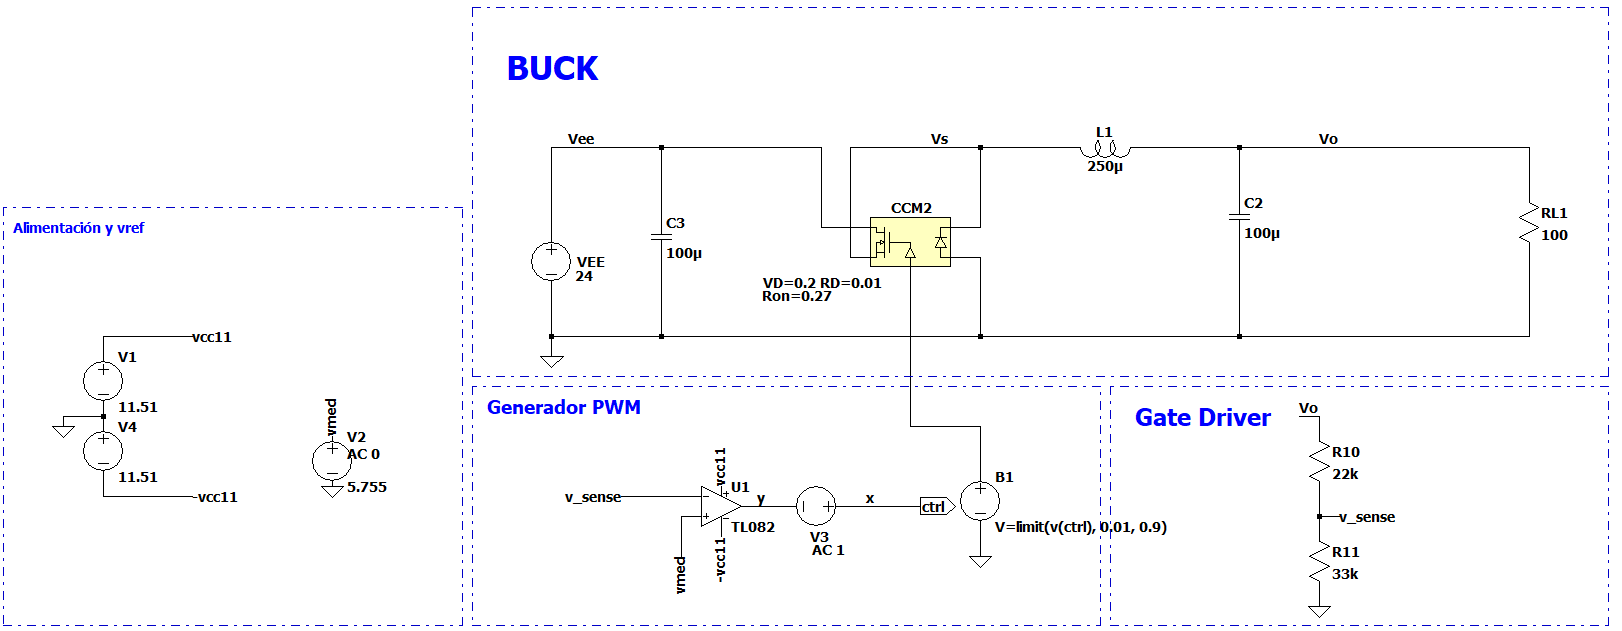
\includegraphics[width=\linewidth]{img/BUCK/sim_compensacion}
		\caption{Archivo de simulación utilizado para evaluar la ganancia de lazo.}
		\label{fig:sim_compensacion}
	\end{figure}
	
	Se utiliza el lazo descompensado, cortado por una fuente AC (V3) sin valor de contínua, y se reemplazan los reguladores lineales por fuentes ideales de contínua para ayudar a la convergencia. Además, se utiliza el TL082 en formato fuente partida, debido a que el componente de fuente promediada (CCM2) opera con valores de tensión 0V-1V.
	
	Para analizar la ganancia de lazo, se debe evaluar la relación entre V(y) y V(x), teniendo en cuenta un signo negativo por utilizar el terminal inversor del operacional:
	
	\begin{equation}
		-\frac{V(y)}{V(x)} = |T|.
	\end{equation}
	
	El gráfico de bode resultante del circuito descompensado se muestra en la figura \ref{fig:sim_descompensado}. Se evalúa para la mínima y máxima carga admisible, con la fuente de tensión $Vee = \SI{30}{V}$.
	
	\begin{figure}[H]
		\centering
		\begin{subfigure}{0.7\textwidth}
			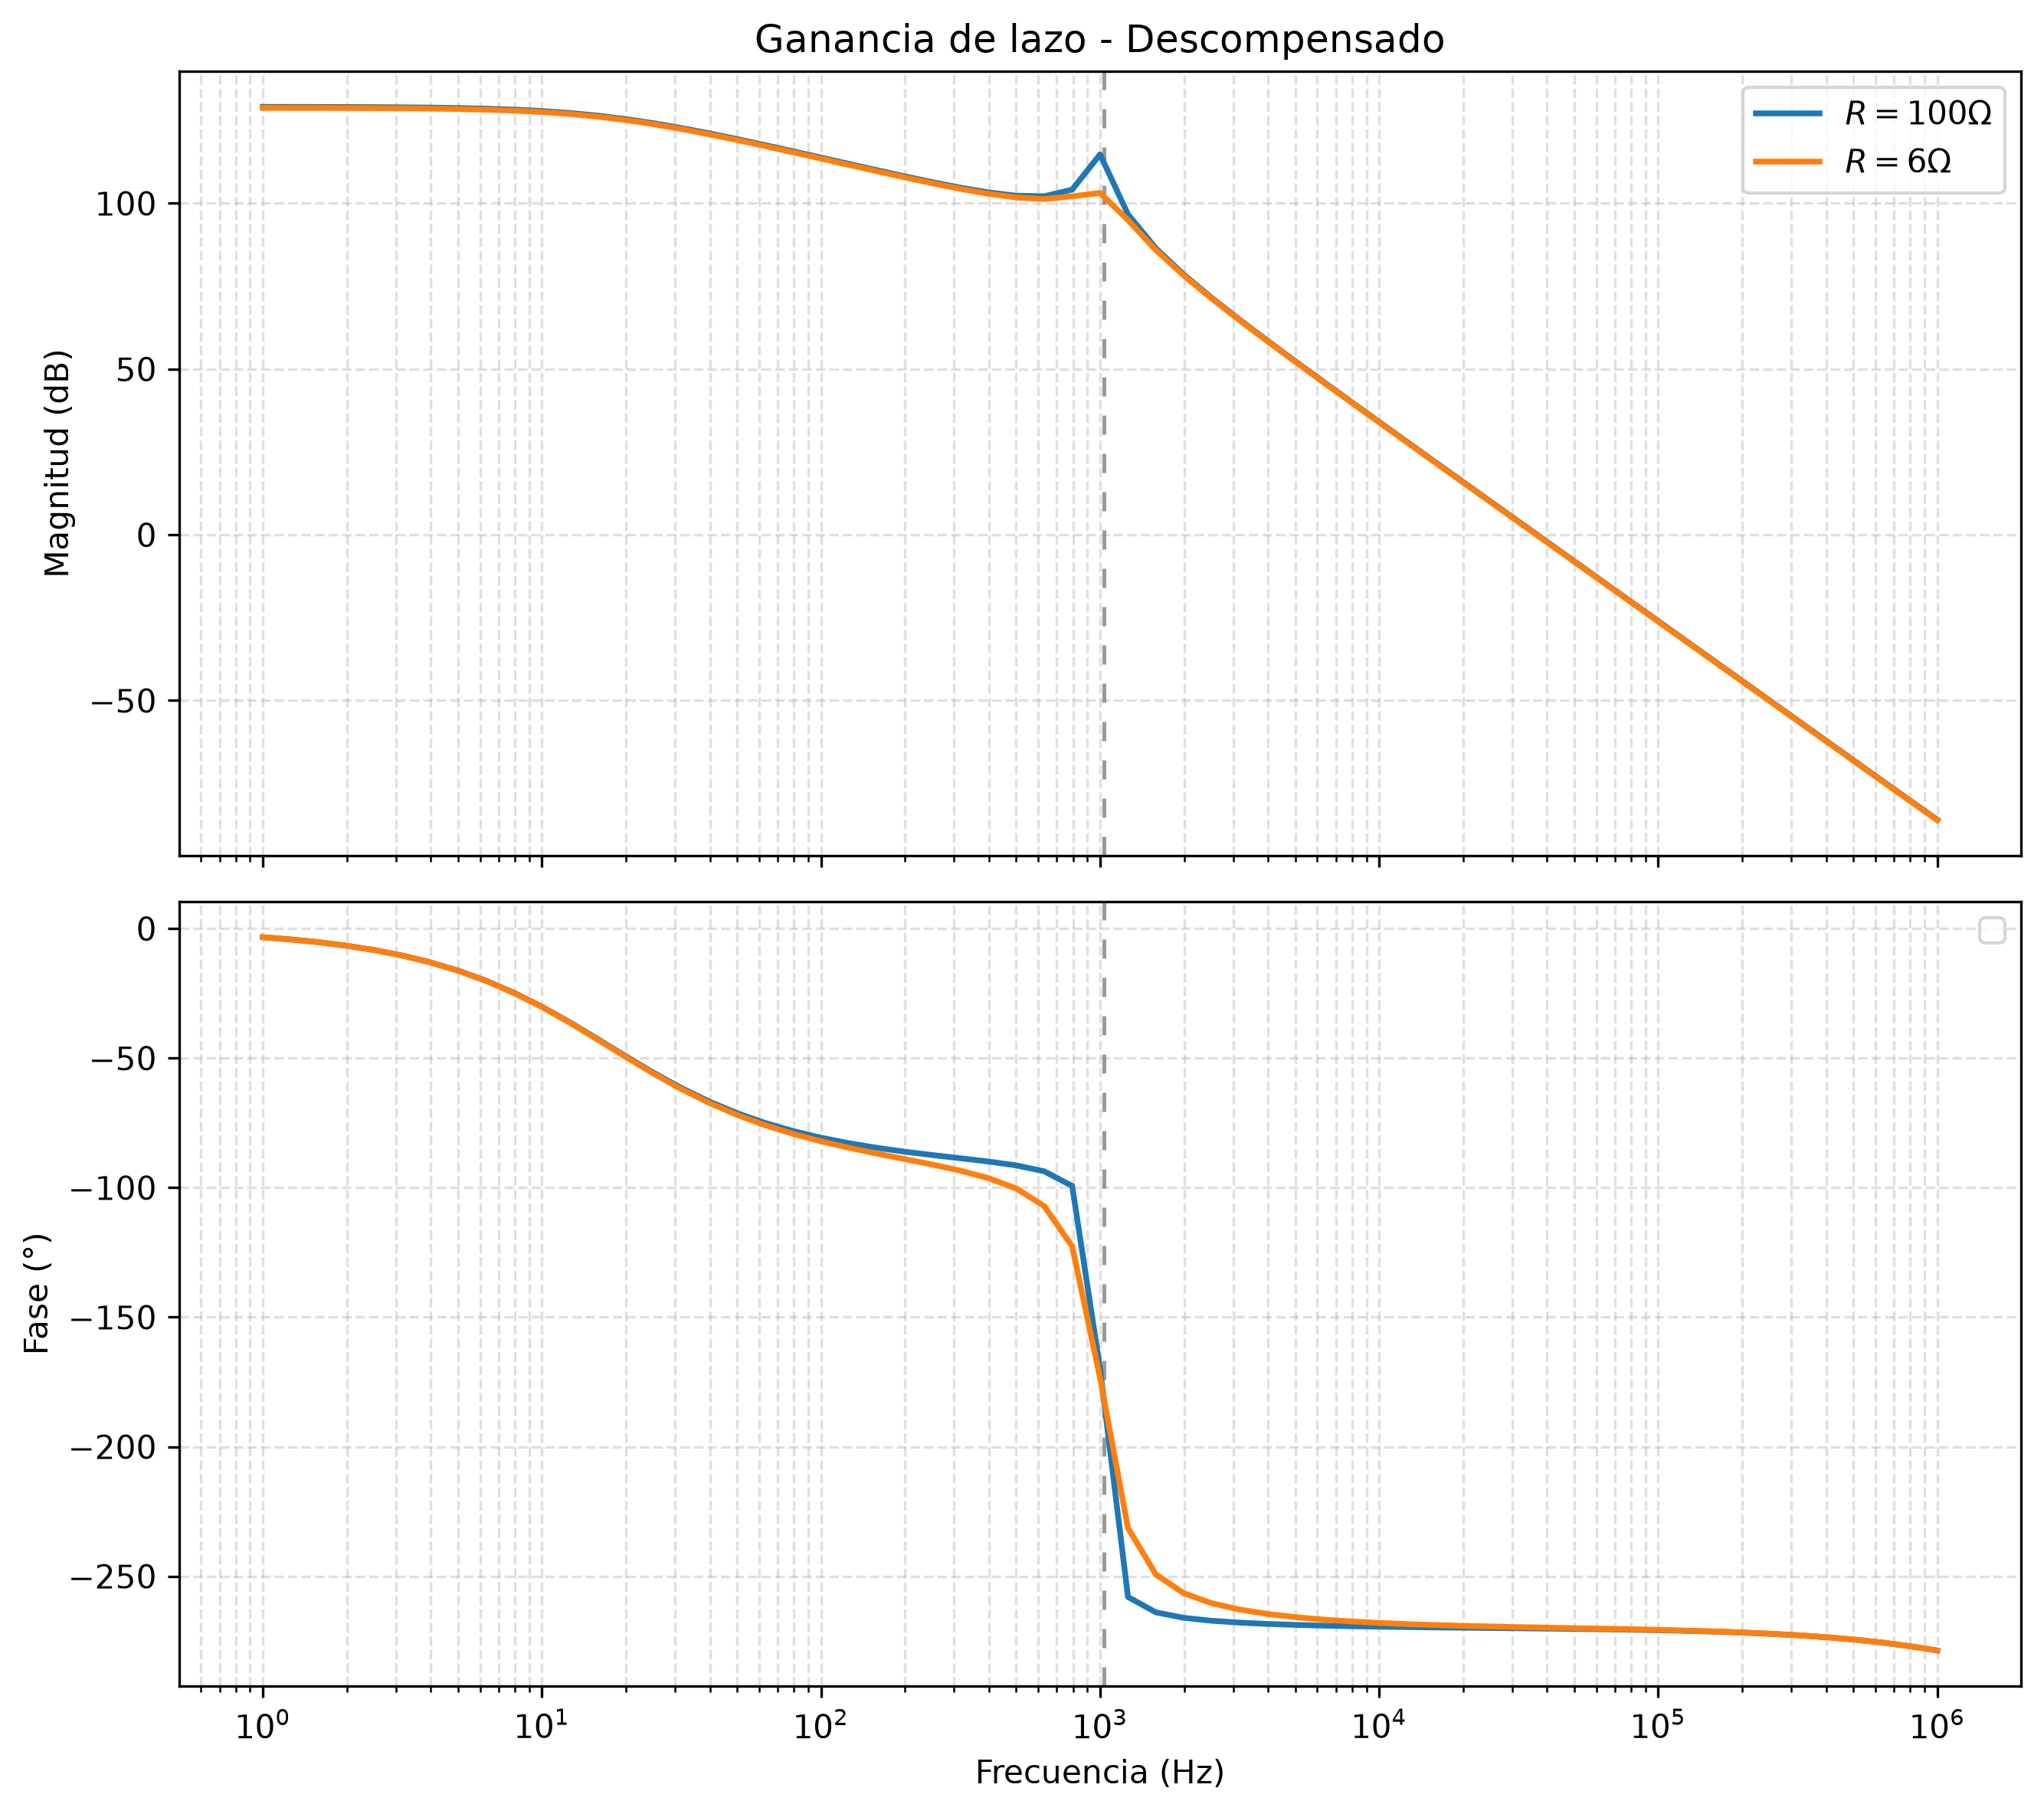
\includegraphics[width=\linewidth]{img/BUCK/bode_descompensado}
			\caption{Ganancia de lazo del circuito descompensado.}
		\end{subfigure}
		\begin{subfigure}{0.7\textwidth}
			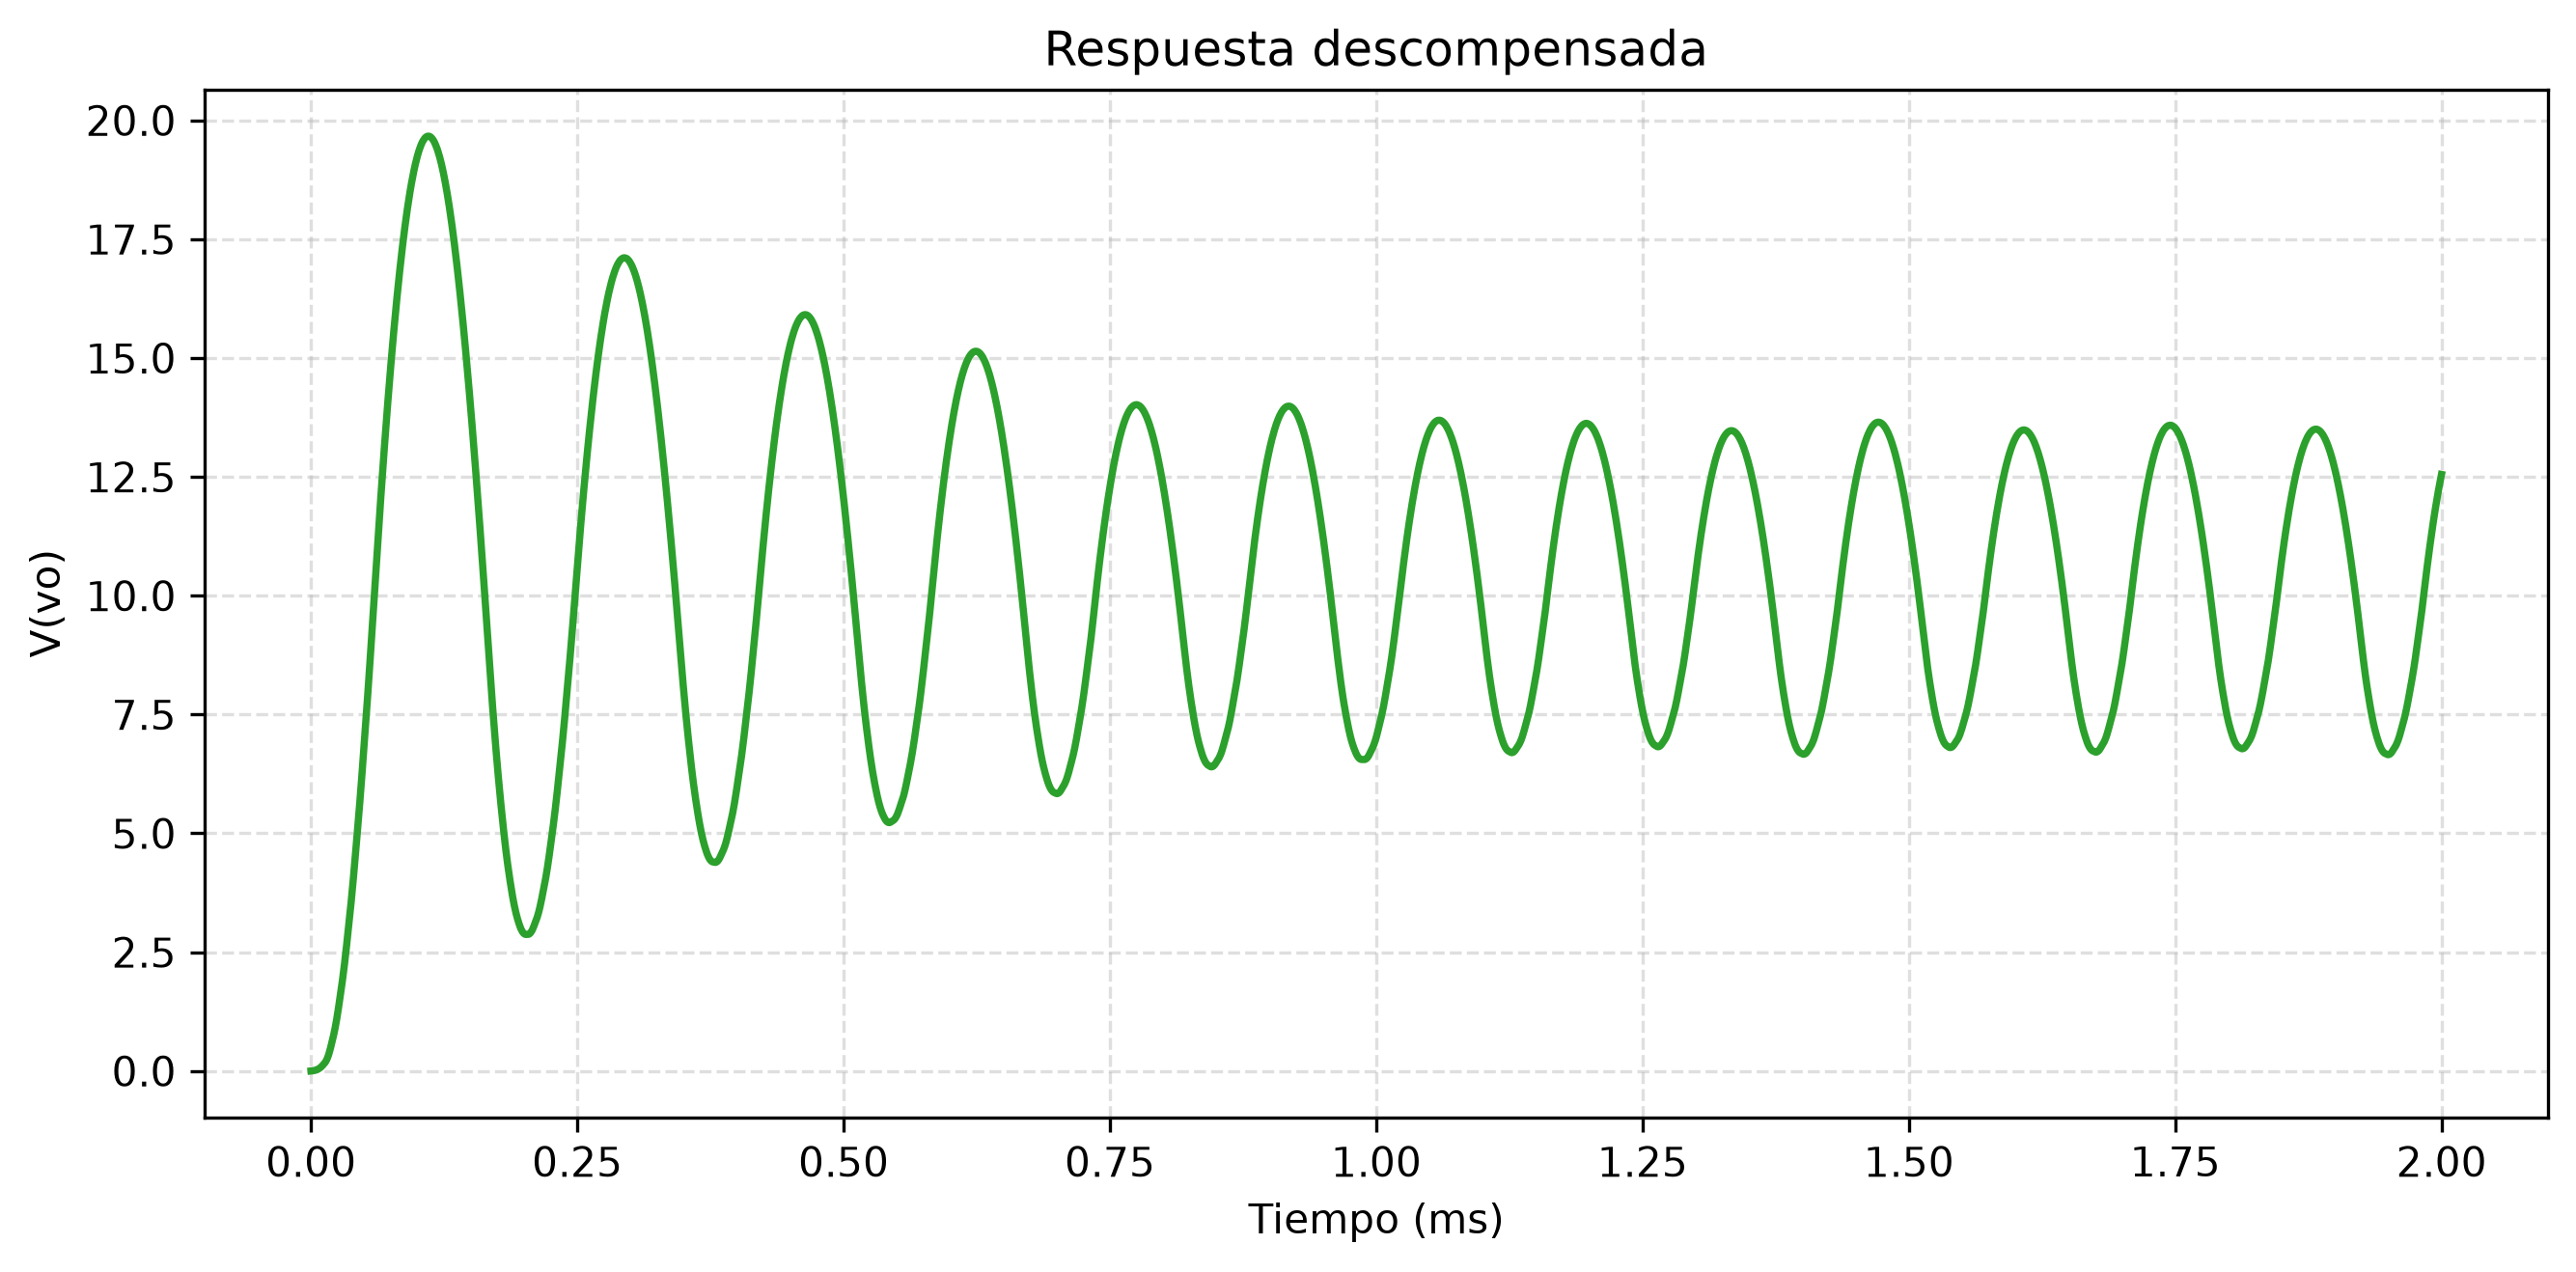
\includegraphics[width=\linewidth]{img/BUCK/respuesta_descompensado}
			\caption{Respuesta temporal del circuito descompensado.}
		\end{subfigure}
		\caption{Análisis temporal y en frecuencia del circuito descompensado.}
		\label{fig:sim_descompensado}
	\end{figure}
	
	La fuente, sin compensar, es fuertemente inestable, con ganancia de lazo abierto \SI{129}{dB}. Para corregir esta situación, se adopta la siguiente técnica:
	
	En primer lugar, se busca utilizar acción integral (polo en el origen) para eliminar el error estacionario. En segundo lugar, se buscará un adelanto de fase con la implementación de un polo y un cero, formando así un amplificador de tipo II (\cite{compensation}), con transferencia.
	
	Adicionalmente, se agrega otra red, esta vez de atraso, que al ser colocada a la entrada del amplificador intercambiará sus polos por sus ceros. Esto forma un amplificador de error de tipo III (figura \ref{fig:compensacion} ). La transferencia final, teniendo en cuenta polos y ceros, tiene la siguiente forma:
	
	\begin{equation}
		|T| = A_{VM} \cdot \frac{\omega_{Z1}}{s} \cdot \frac{1+ \frac{s}{\omega_{Z1}}}{1+ \frac{s}{\omega_{Z2}}} \cdot \frac{1+ \frac{s}{\omega_{P1}}}{1+ \frac{s}{\omega_{P2}}}.
	\end{equation}
	
	Con 
	
	\begin{equation}
		A_{VM} = R_{2}/R_1 \qquad \omega_{Z1} = \frac{1}{R_2 \cdot C_2} \qquad \omega_{Z2} = \frac{1}{\SI{22}{\kilo\ohm} \cdot C_1} \qquad \omega_{P1} = \frac{1}{R_1 \cdot C_1} \qquad \omega_{P2} = \frac{1}{R_2 \cdot C_3}
	\end{equation}
	
	\begin{figure}[H]
		\centering
		\begin{tikzpicture}[transform shape]
			% Paths, nodes and wires:
			\draw (10, 11) to[american resistor, /tikz/circuitikz/bipoles/length=1.08cm, l={$22k\Omega$}] (10, 8);
			\draw (10, 8) to[american resistor, /tikz/circuitikz/bipoles/length=1.08cm, l={$33k\Omega$}] (10, 6);
			\node[tlground] at (10, 6){};
			\node[rground, xscale=-1, yscale=-1](N1) at (10, 11){} node[anchor=south] at ([yshift=0.29cm]N1.text){$V_o$};
			\node[circ] at (10, 8){};
			\draw (10, 8) -- (13, 8);
			\node[op amp](N2) at (14.19, 7.51){} node[anchor=center] at (N2.text){$TL082$};
			\node[inputarrow](N3) at (13, 7.02){} node[anchor=east] at ([xshift=-0.07cm]N3.text){$v_{med}$};
			\node[ground] at (14.107, 6.971){};
			\node[rground, xscale=-1, yscale=-1](N4) at (14.107, 8.029){} node[anchor=south] at ([yshift=0.32cm]N4.text){$V_{11.5V}$};
			\draw (8, 9.5) to[american resistor, /tikz/circuitikz/bipoles/length=1.08cm, l={$R_1$}] (8, 8);
			\draw (8, 8) -- (10, 8);
			\draw (8, 9.5) to[capacitor, /tikz/circuitikz/bipoles/length=0.980cm, l={$C_1$}] (8, 10.75);
			\draw (8, 10.75) -- (10, 10.75);
			\node[circ] at (10, 10.75){};
			\draw (15.38, 7.51) -| (17.75, 7.5);
			\node[inputarrow](N5) at (17.75, 7.5){} node[anchor=west] at ([xshift=0.07cm]N5.text){$Generador\ PWM$};
			\draw (14, 9.5) to[american resistor, /tikz/circuitikz/bipoles/length=1.08cm, l_={$R_2$}] (12, 9.5);
			\draw (14, 9.5) to[capacitor, /tikz/circuitikz/bipoles/length=0.980cm, l={$C_2$}] (15.25, 9.5);
			\draw (15.25, 9.5) -- (15.5, 9.5) -| (15.5, 7.5);
			\draw (12, 9.5) -| (12, 8);
			\draw (13.25, 11) to[capacitor, /tikz/circuitikz/bipoles/length=0.980cm, l_={$C_3$}] (14.5, 11);
			\draw (12, 9.5) -| (12, 11) -- (13.25, 11);
			\draw (14.5, 11) -- (15.5, 11) -| (15.5, 9.5);
			\node[circ] at (15.5, 7.5){};
			\node[circ] at (15.5, 9.5){};
			\node[circ] at (12, 9.5){};
			\node[circ] at (12, 8){};
			\node[shape=rectangle, draw, line width=0.5pt, dash pattern={on 2pt off 2pt}, minimum width=1.982cm, minimum height=3.732cm] at (8, 9.375){};
			\node[shape=rectangle, rotate=-90, draw, line width=0.5pt, dash pattern={on 2pt off 2pt}, minimum width=2.507cm, minimum height=4.323cm] at (13.759, 10.238){};
		\end{tikzpicture}
		\caption{Esquemático del circuito amplificador de error compensado.}
		\label{fig:compensacion}
	\end{figure}
	
	El objetivo será no disminuir el ancho de banda dramáticamente compensando el polo doble en $f \approx \SI{1}{kHz}$ con dos redes de adelanto. Para ello, se fijan valores:
	
	\begin{equation}
		R_1 = \SI{22}{\ohm} \qquad R_2 = \SI{47}{\kilo\ohm} \qquad C_1 = \SI{4.7}{nF} \qquad C_2 = \SI{470}{nF} \qquad C_3 = \SI{470}{pF}
	\end{equation}
	
	Como resultado, se obtienen polos en
	
	\begin{equation}
		\frac{\omega_{P1}}{2\pi} = \SI{1.5}{MHz} \qquad \frac{\omega_{P2}}{2\pi} = \SI{7.2}{\kilo\hertz}
	\end{equation}
	
	y ceros en
	
	\begin{equation}
		\frac{\omega_{Z1}}{2\pi} = \SI{7.2}{Hz} \qquad \frac{\omega_{Z2}}{2\pi} = \SI{1.5}{kHz}.
	\end{equation}
	
	La figura \ref{fig:sim_compensado} muestra la ganancia de lazo y respuesta temporal del sistema, obteniéndose un margen de fase de alrededor de \SI{25}{\deg}.
	
	
	\begin{figure}[H]
		\centering
		\begin{subfigure}{0.7\textwidth}
			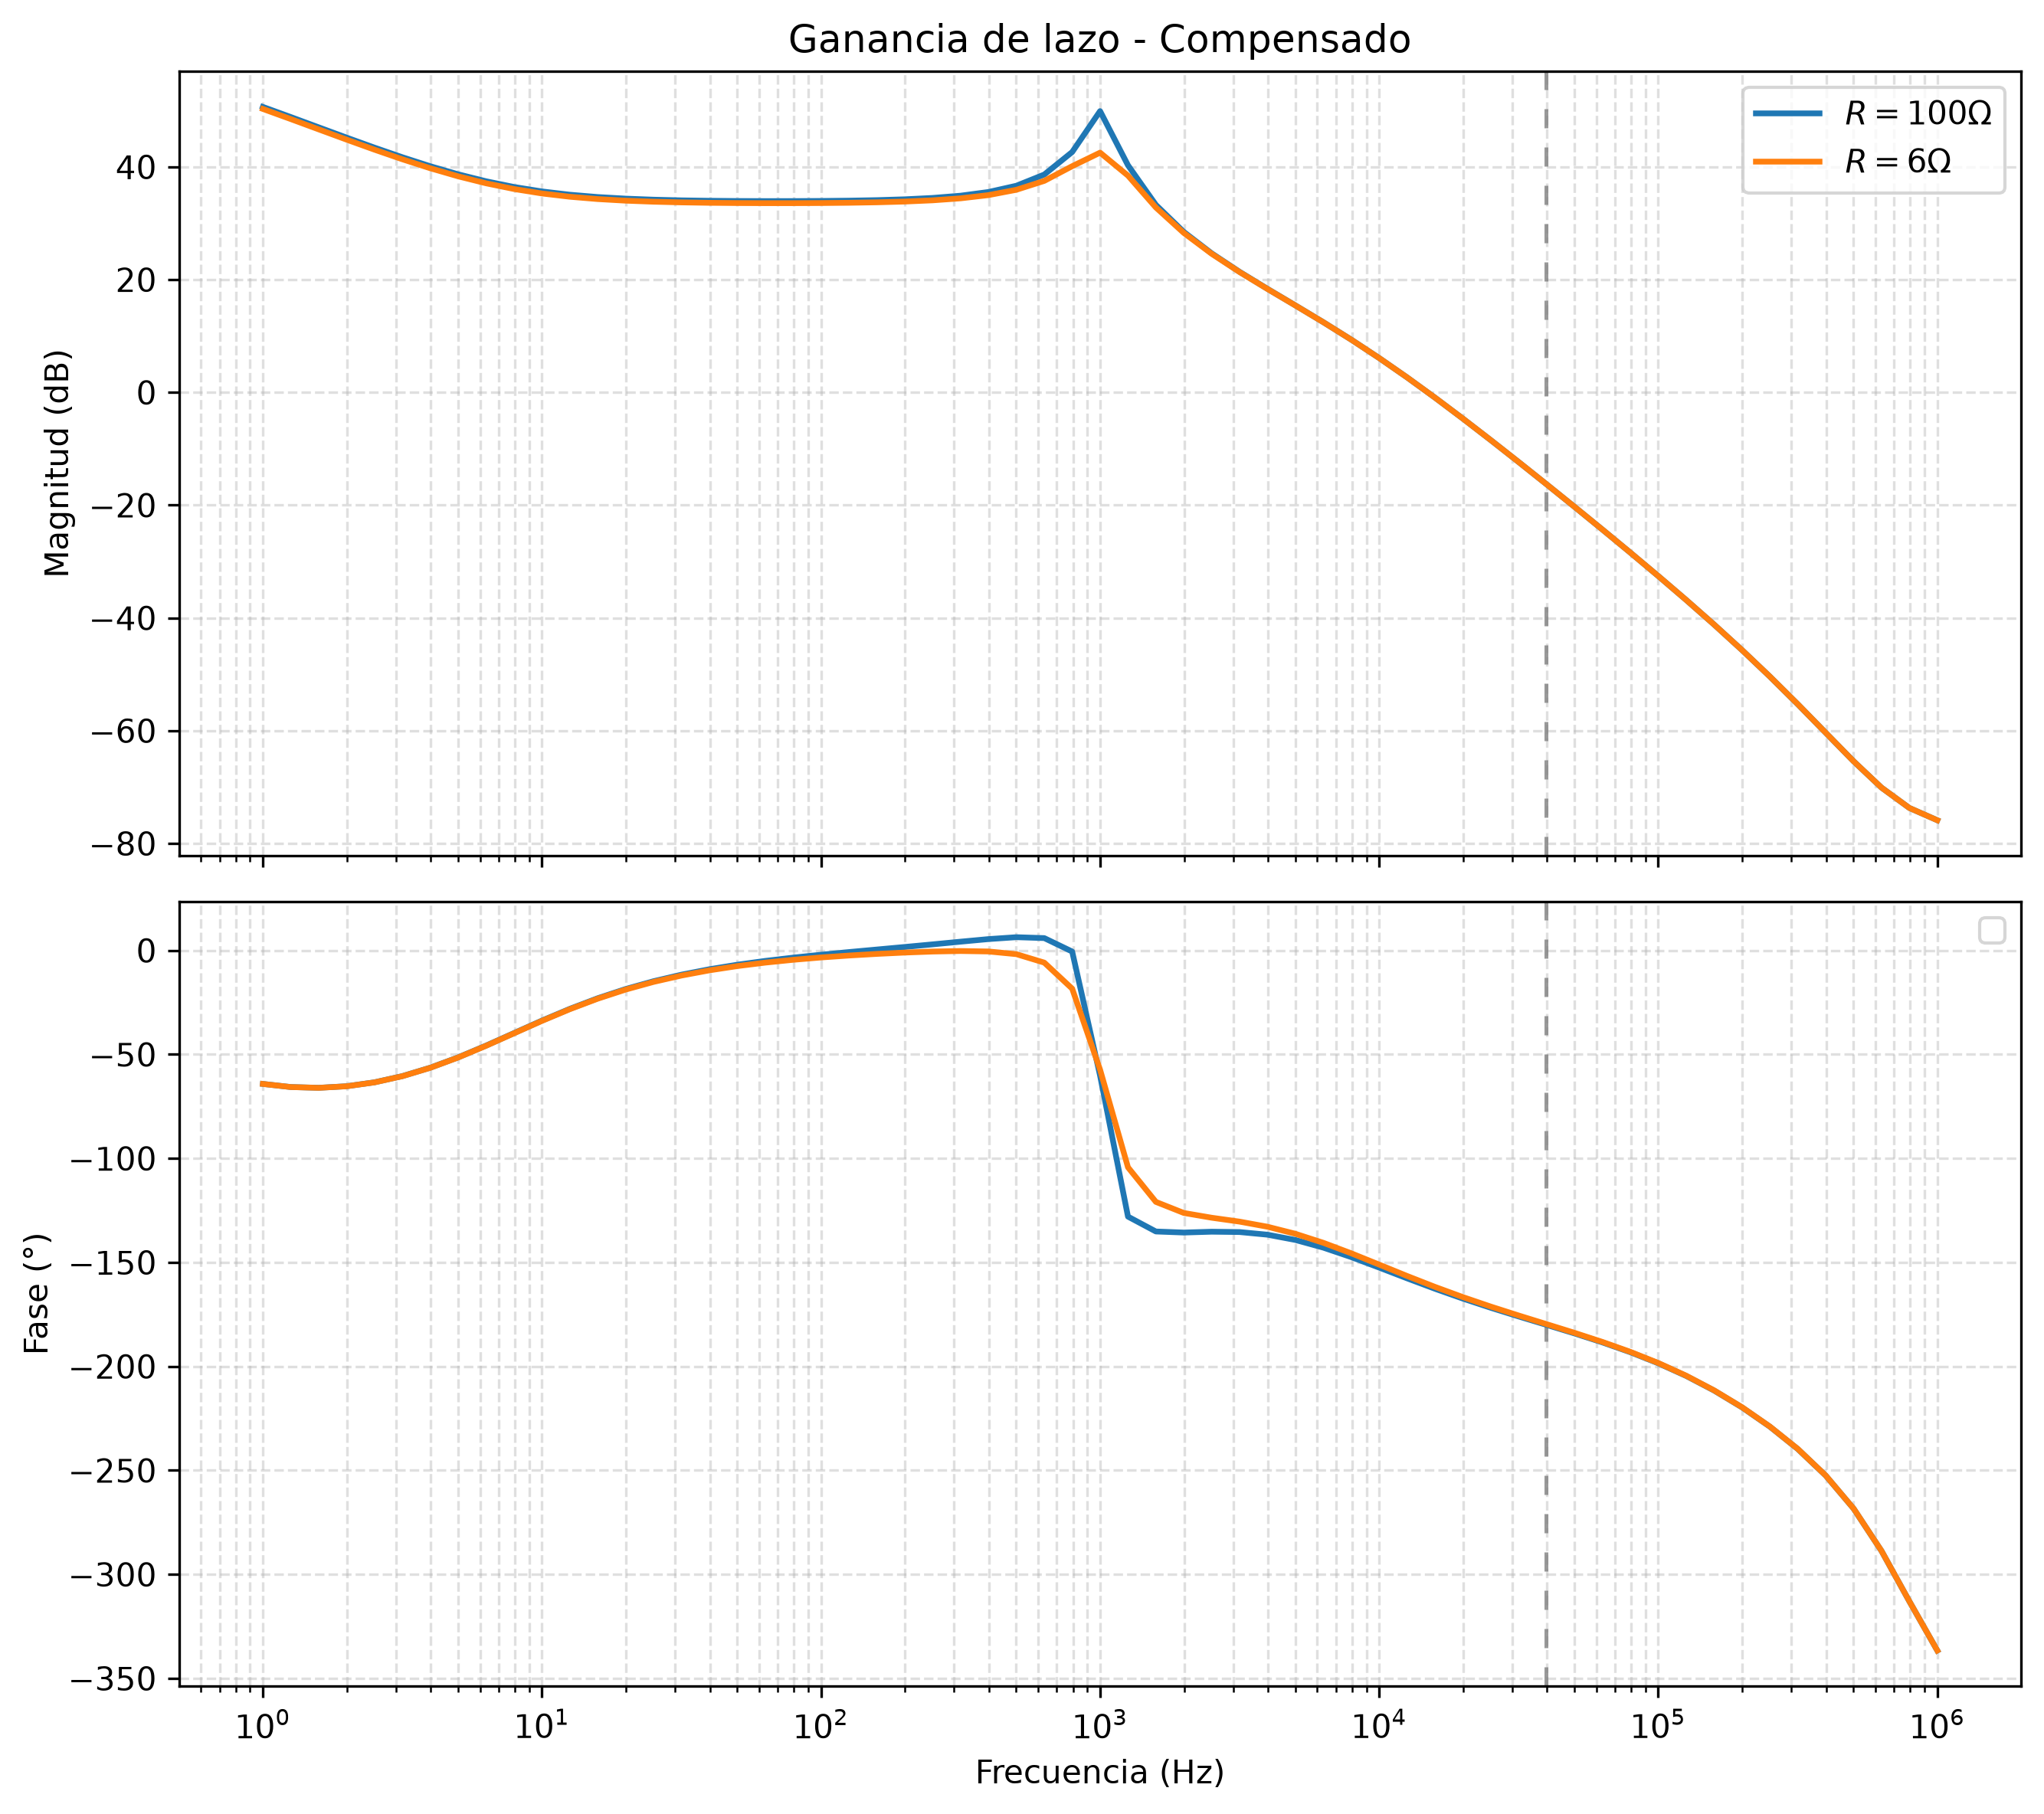
\includegraphics[width=\linewidth]{img/BUCK/bode_compensado}
			\caption{Ganancia de lazo del circuito compensado.}
		\end{subfigure}
		\begin{subfigure}{0.7\textwidth}
			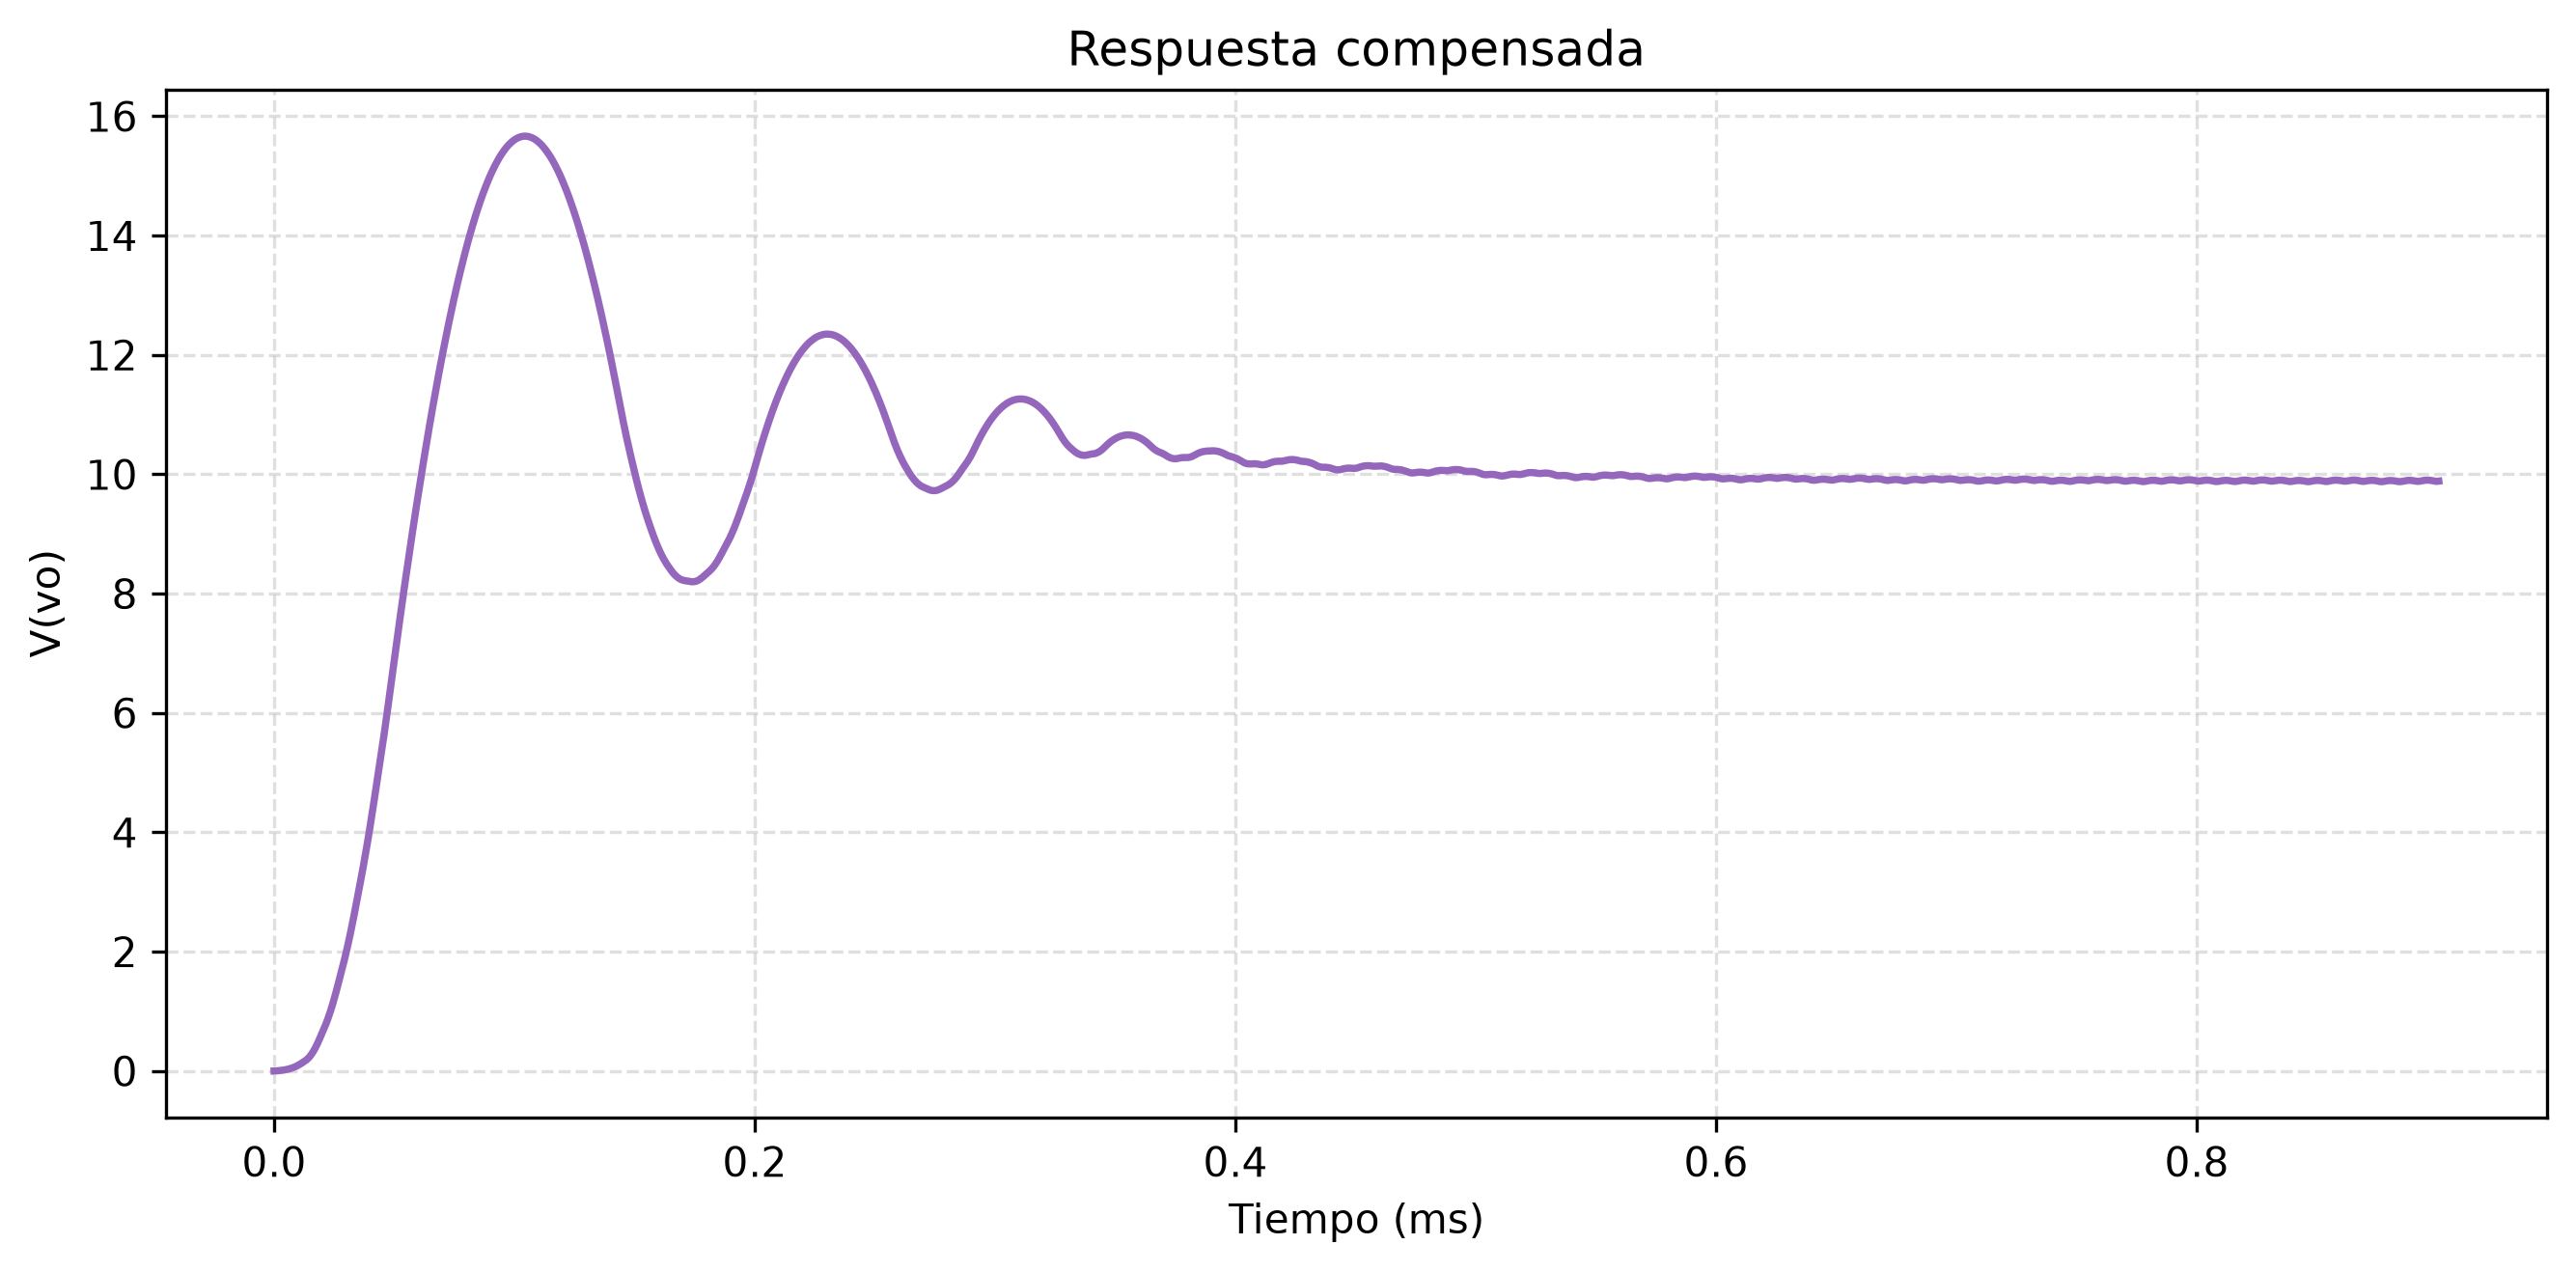
\includegraphics[width=\linewidth]{img/BUCK/respuesta_compensado}
			\caption{Respuesta temporal del circuito compensado.}
		\end{subfigure}
		\caption{Análisis temporal y en frecuencia del circuito compensado.}
		\label{fig:sim_compensado}
	\end{figure}
	
	\subsubsection{Diseño de red \textit{Snubber}}
	
	El diseño de la red \textit{Snubber} depende exclusivamente de las capacidades e inductancias parásitas del circuito. Como tal, es difícil de estimar antes de la implementación.
	
	Para su diseño, se prueba el circuito implementado de la figura \ref{sec:apendice_PCB}, en régimen permanente, y se mide la señal sobre el nodo $V_s$ (figura \ref{fig:vs_snubber}).
	
	\begin{figure}[H]
		\centering
		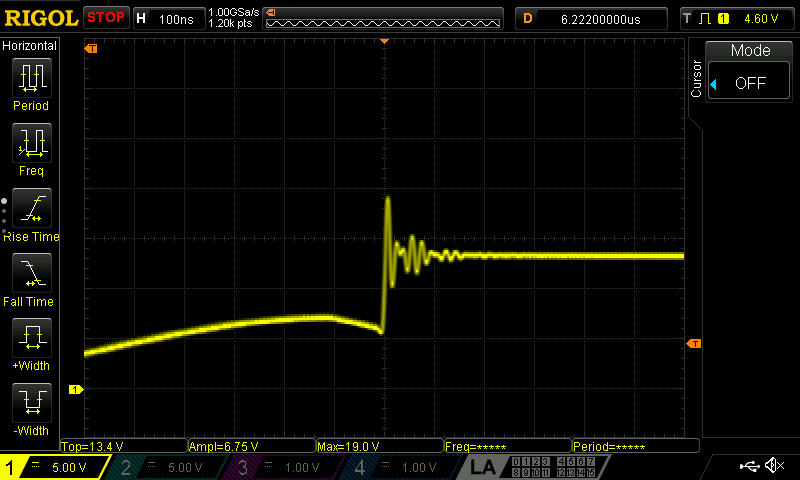
\includegraphics[width=0.7\linewidth]{img/BUCK/ringing2}
		\caption{Efecto \textit{ringing} sobre el nodo de conmutación $V_s$}
		\label{fig:vs_snubber}
	\end{figure}
	
	En base a los resultados experimentales, se diseña la red RC, siguiendo los pasos del manual \cite{toshiba_snubbers}:
	
	\begin{enumerate}
		\item Se observa la frecuencia de la oscilación de la figura \ref{fig:vs_snubber}. $f_s \approx \SI{50}{\mega\hertz}$.
		\item Se calcula la capacidad parásita esperada, que será la resultante de la suma de la capacidad de juntura $C_j$ del diodo de freewheeling y la capacidad total de salida $C_{oss}$ del transistor $Q_2$.
		
		\begin{equation}
			C_p \approx C_j + C_{oss} = \SI{120}{pF} + \SI{70}{pF} = \SI{190}{pF}.
		\end{equation}
		
		\item Se obtiene la inductancia parásita según
		
		\begin{equation}
			L_p \approx \frac{1}{(2\pi f_s)^2 \cdot C_p} = \SI{53.3}{nHy}.
		\end{equation}
		
		\item Finalmente, se calcula la resistencia de la red, que será equivalente a la impedancia
		
		\begin{equation}
			R_{SNB} = \sqrt{\frac{L_p}{C_p}} = \SI{16.7}{\ohm}.
		\end{equation}
	\end{enumerate}
	
	El capacitor de \textit{snubber} será el responsable de la totalidad de la disipación de potencia, y por ende reducción de eficiencia de la fuente. A mayor $C_{SNB}$, mayor atenuación del efecto \textit{ringing}, pero mayor pérdida de eficiencia. En este caso, se escoje una capacidad \SI{220}{pF} cercana a la capacidad parásita.
	
	\begin{equation}
		P_{SNB} = C_{SNB}\cdot V_{IN}^2 \cdot f_{sw} = \SI{220}{pF} \cdot \SI{32}{V} \cdot \SI{130}{\kilo\hertz} = \SI{0.9}{mW}.
	\end{equation}
	
	\subsubsection{Construcción del inductor $L$}
	
	Se diseña el inductor $L$ mediante el método iterativo de EricksonL, cuyas características finales se encuentran en la tabla \ref{tab:diseno_inductor}. El inductor debe diseñarse de forma que opere dentro de la región lineal del núcleo magnético y mantenga sus parámetros eléctricos en las condiciones nominales de operación. Para ello, es necesario considerar las principales limitaciones físicas de un inductor real, las cuales condicionan tanto su desempeño como su eficiencia.
	
	Las características operativas requeridas para el componente se resumen en la Tabla~\ref{tab:especificaciones}:
	
	\begin{table}[h!]
		\centering
		\caption{Parámetros nominales y críticos de diseño.}
		\label{tab:especificaciones}
		\begin{tabular}{lccS}
			\toprule
			\textbf{Parámetro} & \textbf{Símbolo} & \textbf{Unidad} & {\textbf{Valor Nominal}} \\
			\midrule
			Inductancia Nominal         & $L$                        & $\mu \text{H}$ & 250.00 \\
			Frecuencia de Conmutación   & $f_s$                      & \text{kHz}  & 130.00 \\
			Corriente Continua (DC)     & $I_{L_{\text{dc}}}$        & \text{A}    & 1.500  \\
			Corriente Máxima de Pico    & $I_{L_{\text{max}}}$       & \text{A}    & 1.600  \\
			Pérdidas Máximas en el Cobre& $P_{\text{cu}_{\text{max}}}$& \text{W}    & 1.000  \\
			\bottomrule
		\end{tabular}
	\end{table}
	
	
	
	\begin{table}[H]
		\centering
		\renewcommand{\arraystretch}{1.3}
		\begin{tabular}{|l|c|}
			\hline
			\multicolumn{2}{|c|}{\textbf{Diseño del Inductor}} \\
			\hline
			\textbf{Parámetro} & \textbf{Valor} \\
			\hline
			Constante Geométrica $K_g$ & $20.6 \cdot 10^{-2}$\\
			\hline 
			Constante Geométrica $K_{gfe}$ & $2.06 \cdot 10^{-3}$\\
			\hline
			Tipo de material & N87 \\
			\hline
			Tipo de núcleo & EE25 \\
			\hline 
			Sección del núcleo $A_c$ & 0.36 $\, cm^2 $\\
			\hline 
			Área de ancho de la bobina : $ W_A$ & 0.500$\, cm^2 $\\
			\hline
			Longitud media por vuelta : $MLT $ & 4.7 $\, cm $ \\
			\hline 
			Peso del núcleo: $g$ & 15.1 $\, g$\\
			\hline
			Entre hierro (gap) & $l_g=\SI{0.17}{\milli\meter}$ \\
			\hline
			Número de vueltas & $n_l=37$ \\
			\hline
			Tipo de alambre & AWG\#25 \\
			\hline
			Sección transversal del conductor $A_w$ & $1,623 \, \cdot 10^{-3} cm^2$\\
			\hline
		\end{tabular}
		\caption{Parámetros de diseño del inductor de $L=\SI{50}{\micro\henry}$}
		\label{tab:diseno_inductor}
	\end{table}
	
	
	
	
	
	\begin{figure}[H]
		\centering
		
		\begin{minipage}{0.28\textwidth}
			\centering
			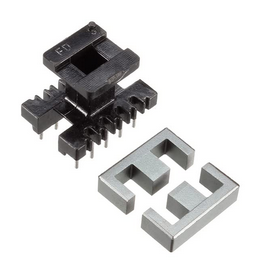
\includegraphics[width=\linewidth]{img/diseño_inductor/nucleo_EE19}
		\end{minipage}
		\hfill
		\begin{minipage}{0.65\textwidth}
			\small
			El núcleo \textbf{EE25} está compuesto por dos mitades con forma de
			letra \textit{E}, cuya unión conforma un circuito magnético cerrado.
			La denominación ``EE'' hace referencia a esta geometría, mientras que
			el número ``25'' identifica el tamaño principal del núcleo, de
			aproximadamente \SI{25}{mm}. Este tipo de núcleo de ferrita es
			ampliamente utilizado en inductores y transformadores de fuentes
			conmutadas debido a su facilidad de bobinado y buen aprovechamiento
			del flujo magnético.
		\end{minipage}
		
		\caption{Núcleo EE25 sin ensamblar.}
		\label{fig:nucleoee19}
		
		
	\end{figure}
	\begin{figure}[H]
		\centering
		
		\begin{minipage}{0.28\textwidth}
			\centering
			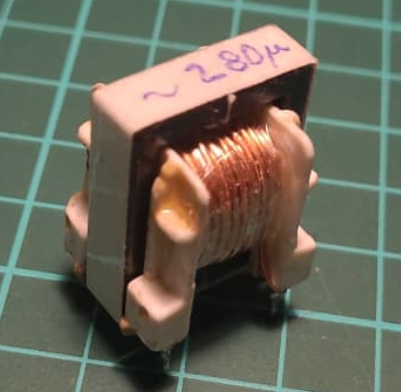
\includegraphics[width=0.7\linewidth]{img/BUCK/inductor_fabricado}\end{minipage}
		\hfill
		\begin{minipage}{0.65\textwidth}
			
			El inductor fue construido realizando el bobinado de forma manual sobre el carrete. Para reducir las pérdidas por efecto pelicular a la frecuencia de conmutación, se emplearon dos conductores esmaltados conectados en paralelo. Finalmente, se incorporó un entrehierro (\textit{gap}) mediante una lámina aislante calibrada entre ambas mitades del núcleo, aumentando la reluctancia del circuito magnético y disminuyendo la inductancia hasta el valor de diseño.
			
		\end{minipage}
		
		\caption{Núcleo EE25 ensamblado.}
		\label{fig:nucleoee25_ensaamblado}
	\end{figure}
	
	
	\subsubsection{Profundidad de penetración}
	
	Debido a la elevada frecuencia de conmutación del convertidor, la corriente alterna tiende a concentrarse cerca de la superficie del conductor, fenómeno conocido como efecto pelicular (\textit{skin effect}). Cuando el radio del conductor supera la profundidad de penetración, la resistencia efectiva aumenta y, en consecuencia, también las pérdidas por conducción. Para mitigar este efecto se decidió emplearse conductores de menor diámetro conectados en paralelo o cable tipo \textit{Litz}, incrementando el área efectiva de conducción para la componente alterna de la corriente.
	
	La profundidad de penetración viene dada por:
	
	\begin{equation}
		\delta=\sqrt{\frac{2\rho}{\omega\mu}}
		\label{eq:skin_depth}
	\end{equation}
	
	donde:
	
	\begin{itemize}
		\item $\rho = 1.72\times10^{-8}\,\Omega\cdot\mathrm{m}$ es la resistividad del cobre.
		\item $\mu=\mu_0\mu_r$ es la permeabilidad magnética del conductor.
		\item $\mu_0=4\pi\times10^{-7}\,\mathrm{H/m}$.
		\item $\mu_r\simeq1$ para el cobre.
		\item $\omega=2\pi f$.
	\end{itemize}
	
	Para una frecuencia de conmutación de
	
	\[
	f=130\,\mathrm{kHz},
	\]
	
	se obtiene
	
	\[
	\omega=2\pi(130\times10^3)
	=8.17\times10^5\;\mathrm{rad/s}.
	\]
	
	Reemplazando en la ecuación \eqref{eq:skin_depth},
	
	\begin{equation}
		\delta=
		\sqrt{
			\frac{
				2(1.72\times10^{-8})
			}{
				(8.17\times10^5)
				(4\pi\times10^{-7})
			}
		}
		\simeq1.84\times10^{-4}\,\mathrm{m}
	\end{equation}
	
	es decir,
	
	\begin{equation}
		\boxed{\delta\simeq0.184\ \mathrm{mm}}
	\end{equation}
	
	Por lo tanto, para minimizar las pérdidas por efecto pelicular se recomienda que el radio del conductor sea del orden de la profundidad de penetración o menor, es decir,
	
	\[
	r\lesssim\delta,
	\]
	
	lo que equivale aproximadamente a un diámetro máximo de
	
	\[
	d\lesssim2\delta
	\simeq0.37\ \mathrm{mm}.
	\]
	
	En caso de requerirse una sección transversal mayor, resulta conveniente emplear varios conductores en paralelo o cable Litz.
	
	\subsubsection{Densidad de corriente}
	
	La sección transversal del conductor debe dimensionarse de manera que la densidad de corriente permanezca dentro de los valores recomendados para limitar el incremento de temperatura del bobinado y evitar pérdidas excesivas por efecto Joule.
	
	La densidad de corriente se calcula mediante
	
	\begin{equation}
		\sigma_{I_L}=\frac{I_{L,\max}}{A_w}
		\label{eq:densidad_corriente}
	\end{equation}
	
	donde:
	
	\begin{itemize}
		\item $I_{L,\max}$ es la corriente máxima que circula por el devanado.
		\item $A_w$ es el área de la sección transversal del conductor.
	\end{itemize}
	
	Para el conductor seleccionado se obtiene
	
	\[
	\sigma_{I_L}
	=
	\frac{I_{L,\max}}{A_w}
	\quad
	[\mathrm{A/mm^2}].
	\]
	
	Se verifica además que
	
	\begin{equation}
		\sigma_{I_L}
		<
		\sigma_{I_L,\mathrm{esp}}
		=
		5\;\mathrm{A/mm^2},
	\end{equation}
	
	cumpliéndose el criterio de diseño adoptado para la densidad máxima de corriente en el conductor.
	
	Por lo tanto, la sección del alambre seleccionada resulta adecuada, limitando las pérdidas óhmicas y evitando
	\subsubsection{Saturación del núcleo} 
	
	El núcleo magnético debe operar por debajo de la densidad de flujo de saturación del material. De esta manera se asegura que la inductancia permanezca prácticamente constante y se evita la disminución abrupta de la inductancia, el aumento de la corriente y las pérdidas asociadas al funcionamiento en saturación.
	
	
	
	Considerando que la reluctancia del circuito magnético está dominada por el entrehierro, la intensidad de campo magnético en el mismo viene dada por
	
	\begin{equation}
		H_g=\frac{N_LI_{L,\max}}{l_g},
		\label{eq:H_gap}
	\end{equation}
	
	donde:
	
	\begin{itemize}
		\item $N_L$ es el número de espiras del inductor,
		\item $I_{L,\max}$ es la corriente máxima del devanado,
		\item $l_g$ es la longitud efectiva del entrehierro.
	\end{itemize}
	
	Como en el entrehierro
	
	\[
	B=\mu_0H,
	\]
	
	la densidad de flujo máxima resulta
	
	\begin{equation}
		B_{\max}
		=
		\mu_0
		\frac{N_LI_{L,\max}}{l_g},
		\label{eq:Bmax_gap}
	\end{equation}
	
	donde
	
	\[
	\mu_0=4\pi\times10^{-7}\ \mathrm{H/m}.
	\]
	
	Reemplazando los valores de diseño,
	
	\[
	B_{\max}
	=
	\mu_0
	\frac{N_LI_{L,\max}}{l_g}
	= 0.003 \, \mu
	\ \mathrm{T}.
	\]
	
	Finalmente, se verifica que
	
	\begin{equation}
		B_{\max}
		<
		B_{\mathrm{sat}} = 300 \, mT,
	\end{equation}
	
	cumpliéndose el criterio de diseño adoptado.
	\subsubsection{Resistividad del cobre}
	
	Al seleccionar un conductor, en este caso el cobre, junto con su sección se establece una resistencia al paso de cargas. De esta forma se produce la resistencia $R_cu$ como:
	
	\begin{equation}
		R_{cu} =  \frac{(\rho_{cu} \cdot nl \cdot MLT)}{Aw} = 0.087  \; \Omega\
	\end{equation} 
	
	En la ecuación, $\rho_{cu} $ representa la resistividad eléctrica del cobre, nl el número de espiras del devanado, MLT (Mean Length per Turn) la longitud media de una espira y $A_w$ el área de la sección transversal del conductor empleado.
	
	
	
	Se debe considerar un valor de resistencia máximo como limite superior, en este caso fue el valor dado por la ley de Joule aplicada al devanado del inductor : 
	$ {R_{cu}}_{[max]} = \left( \frac{P_{\text{cu}_{\max}}}{I_{L_{\text{dc}}}} \right)^2 = 0,390\, \Omega$
	
	Al realizar un bobinado del tipo paralelo la sección del cobre disminuye, lo que favorece una distribución más uniforme de la corriente a altas frecuencias. Si se mantiene constante la sección total de cobre, la resistencia en corriente continua permanece prácticamente inalterada, mientras que la resistencia en corriente alterna disminuye debido a la reducción del efecto pelicular. Con lo cual la expresión sigue siendo valida y se cumple lo requerido.	
	
	\subsubsection{Diseño PCB de la buck en lazo abierto}
	
	Se diseño el circuito \textit{buck} de forma que se pueda utilizar a lazo abierto modularizando la placa, en la figura \ref{fig:bucksolopcb} se puede observar el modelo en tres dimensiones del sector de la placa correspondiente al circuito \textit{buck}. 
	
	\begin{figure}[H]
		\centering
		
\includegraphics[width=0.7\linewidth]{img/buck/buck_solo_pcb}
		\caption{Diseño del PCB del circuito buck.}
		\label{fig:bucksolopcb}
	\end{figure}
	
	\subsection{Diseño PCB de circuito PWM}
	
	
	Se implementa el circuito en placa impresa. Notar que se deja espacio para el cálculo e implementación de la compensación del lazo realimentador (ver $C_4$ y $C_2$ en la figura \ref{sec:apendice_PCB}), para el futuro cierre del lazo. Se realizo un diseño simple faz a modo prototipo con ciertas conexiones cableadas en la capa superior y \textit{jumpers} para testeo como se aprecia en la figura \ref{fig:pwmpcb}, luego se implemento mediante transferencia térmica y corrosión de cobre sobrante de la placa con el uso de percloruro férrico obteniendo la placa Fig. \ref{fig:pcbbuck}.
	
	\begin{figure}[H]
		\centering
		
\includegraphics[width=0.7\linewidth]{img/buck/pwm_pcb}
		\caption{Modelo 3D del PWM en circuito impreso.}
		\label{fig:pwmpcb}
	\end{figure}
	
	\subsubsection{Diseño PCB Completo}
	
	\begin{figure}[H]
		\centering
		
\includegraphics[width=0.7\linewidth]{img/buck/PCB_frente}
		\caption{}
		\label{fig:pcbfrente}
	\end{figure}
	
	\begin{figure}[H]
		\centering
		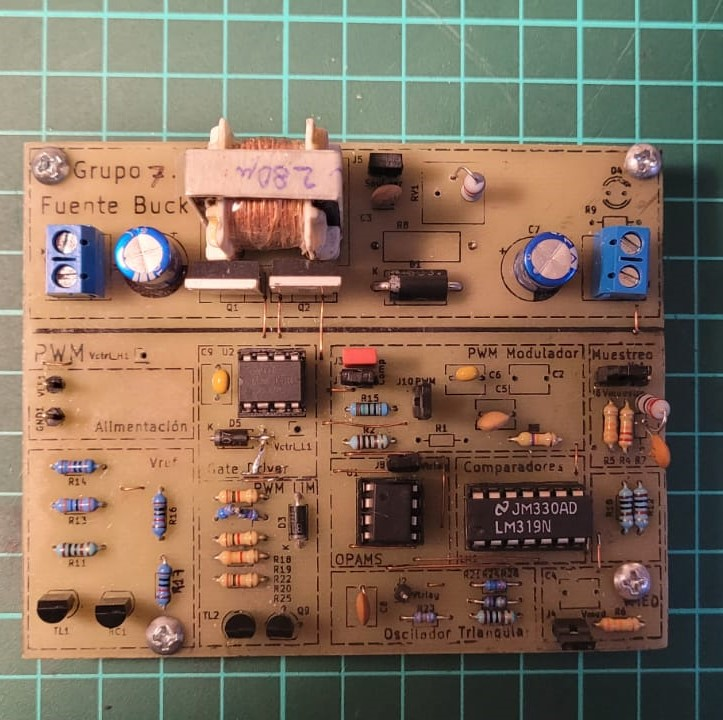
\includegraphics[width=0.7\linewidth]{img/BUCK/pcb_buck}
		\caption{}
		\label{fig:pcbbuck}
	\end{figure}
	
	\subsection{Regulador de baja caída (LDO,Low Dropout Regulator)}
	
	\subsubsection{Especificaciones}
	\FloatBarrier
	El propósito de esta etapa es regular la tensión de salida de la fuente conmutada de forma precisa, sacrificando la eficiencia. Se espera de esta etapa las especificaciones de la tabla \ref{tabla:especificaciones_ldo}.
	
	\begin{table}[h]
		\centering
		\renewcommand{\arraystretch}{1.5}
		\begin{tabular}{|p{3cm}|l|p{5cm}|c|c|c|c|}
			\hline
			\textbf{Característica} & \textbf{Símbolo} & \textbf{Condiciones de prueba} & \textbf{Min.} & \textbf{Tip.} & \textbf{Max.} & \textbf{Unidades} \\
			\hline
			
			\multicolumn{7}{|l|}{\textbf{Especificaciones regulador lineal Vo}} \\
			\hline
			
			Vo exactitud y regulación de carga & Vo & $\SI{100}{mA} < I_{out} < \SI{1.5}{A}$ \break $VREG = \SI{9.5}{V}$ & 4,9 & 5 & 5,1 & V \\
			\hline
			
			Vo rango de capacidad de carga & COUT(Vo) &  & 1,0 & 2,2 & 15,0 & \si{\micro\farad} \\
			\hline
			
			Io corriente límite & ILIM(Vo) &  &  & 1,5 &  & A \\
			\hline
			
			Corriente de foldback & IFBK &  &  & 400 &  & \si{mA} \\
			\hline
		
			%\multirow{2}{3cm}{Vo startup time} & t(start) & $C = \SI{2.2}{\micro\farad},\ I = \SI{100}{\milli\ampere}$ &  &  &  & ms \\
			%\cline{2-7}
			% & t(start) & $C = \SI{2.2}{\micro\farad},\ I = \SI{100}{\milli\ampere}$ &  &  &  & ms \\
			%\hline
		\end{tabular}
		
		\caption{Especificaciones del regulador lineal LDO.}
		\label{tabla:especificaciones_ldo}
	\end{table}
	
	\subsubsection{Implementación}
	
Para la implementación, se utilizará un transistor de paso, responsable de disipar la potencia de recorte, realimentado por tensión y corriente, y se modela la entrada de tensión pre-regulada con una componente continua y una alterna de acuerdo a la figura \ref{fig:bloques_ldo}.

\begin{figure}[h]
	\centering
\begin{tikzpicture}[transform shape]
	% Paths, nodes and wires:
	\node[op amp, xscale=-0.78, yscale=-0.78] at (14.572, 8.132){};
	\draw (11, 12) to[american voltage source, mirror, l_={$V_{cc}$}] (11, 10);
	\draw (11, 12) to[sinusoidal voltage source, l={$v_{ac}$}] (11, 14);
	\node[pigfete, rotate=90](N1) at (17.27, 14){} node[anchor=south] at (N1.text){$T_p$};
	\draw (11, 14) -- (16.5, 14);
	\node[spdt, rotate=-90] at (17, 11.5){};
	\draw (21, 12) to[american resistor, /tikz/circuitikz/bipoles/length=0.840cm, l={$R_L$}] (21, 10);
	\draw (15, 12.75) to[push button] (16.5, 12.75);
	\draw (16.5, 12.75) -| (17, 13.02);
	\draw (15, 12.75) -- (14.5, 12.75) -- (14.5, 14);
	\draw (12.5, 10.75) to[full ZZener diode, mirror, /tikz/circuitikz/bipoles/length=0.700cm] (12.5, 12.25);
	\draw (12.5, 12.25) -| (12.5, 14);
	\draw (12.5, 10.75) |- (11, 10);
	\draw (21, 10) -- (12.5, 10);
	\node[shape=rectangle, draw, line width=1pt, minimum width=0.965cm, minimum height=1.465cm] at (12.5, 11.5){};
	\draw (13, 11.5) -- (13.5, 11.5);
	\node[circ](N2) at (13.5, 11.5){} node[anchor=west] at (N2.text){$v_{ref}$};
	\draw (17, 12.095) -| (17, 12.75);
	\draw (15.5, 7.75) -- (15.75, 7.75);
	\node[circ](N3) at (15.75, 7.75){} node[anchor=west] at (N3.text){$v_{ref-t}$};
	\node[shape=rectangle, draw, line width=1pt, minimum width=1.965cm, minimum height=1.215cm] at (18.5, 8.125){};
	\draw (19, 8.5) -| (20, 12) -- (21, 12);
	\draw (19, 7.75) -| (21, 10);
	\draw (18, 8.5) to[american controlled voltage source, mirror, /tikz/circuitikz/bipoles/length=0.700cm] (18, 7.75);
	\draw (18, 8.5) |- (15.5, 8.514);
	\draw (18, 7.75) -- (17.25, 7.75) -- (17, 7.75) -| (17, 7.25);
	\node[op amp, xscale=-0.78, yscale=-0.78] at (14.572, 6.257){};
	\draw (15.5, 5.875) -- (15.75, 5.875);
	\node[circ](N4) at (15.75, 5.875){} node[anchor=west] at (N4.text){$v_{ref-c}$};
	\node[shape=rectangle, draw, line width=1pt, minimum width=1.965cm, minimum height=1.215cm] at (18.5, 6.25){};
	\draw (18, 6.625) to[american controlled voltage source, mirror, /tikz/circuitikz/bipoles/length=0.700cm] (18, 5.875);
	\draw (18, 6.625) |- (15.5, 6.639);
	\draw (18, 5.875) -- (17.25, 5.875) -- (17, 5.875) -| (17, 5.375);
	\draw (19, 6.5) -| (22, 12.5) -- (21, 12.5);
	\draw (21, 13.25) -- (22.75, 13.25) |- (19, 6);
	\draw (19, 6.5) -| (19, 6);
	\draw (21, 12) -| (21, 12.5);
	\draw (21, 13.25) |- (18.04, 14);
	\node[tlground] at (17, 5.375){};
	\node[tlground] at (17, 7.25){};
	\draw (13.644, 6.257) -| (13, 6.25) -| (13, 9.75) -- (16.5, 9.75) -| (16.685, 10.905);
	\draw (13.644, 8.132) |- (17.25, 9.25) -| (17.315, 10.905);
	\node[shape=rectangle, minimum width=0.715cm, minimum height=0.715cm] at (18.5, 9.125){} node[anchor=north west, align=left, text width=0.327cm, inner sep=6pt] at (18.125, 9.5){$f_v$};
	\node[shape=rectangle, minimum width=0.715cm, minimum height=0.715cm] at (18.5, 5.25){} node[anchor=north west, align=left, text width=0.327cm, inner sep=6pt] at (18.125, 5.625){$f_A$};
	\node[circ] at (19, 7.75){};
	\node[circ] at (19, 8.5){};
	\node[circ] at (14.5, 14){};
	\node[circ] at (12.5, 14){};
	\node[circ] at (12.5, 10){};
	\node[circ] at (17, 12.75){};
	\node[circ] at (21, 12){};
	\node[circ] at (21, 10){};
	\node[shape=rectangle, draw, line width=1pt, minimum width=1.59cm, minimum height=1.31cm] at (17, 11.5){};
	\node[shape=rectangle, draw, line width=1pt, minimum width=1.715cm, minimum height=0.715cm] at (15.75, 12.875){};
	\draw (11, 10) -| (11, 9.75);
	\node[tlground] at (11, 9.75){};
\end{tikzpicture}
	\caption{Circuito simplificado del circuito regulador LDO.}
	\label{fig:bloques_ldo}
\end{figure}
\FloatBarrier
\subsubsection{El transistor de paso (Tipo MOS)}
\FloatBarrier
La elección del transistor de paso es nuestro primer paso de diseño, y para su elección deben tenerse en cuenta los siguientes puntos:

\textbf{Canal} \par

El canal del transistor determinará sobre dónde se efectúa el control. 

\begin{figure}[h]
	\centering
	\begin{tikzpicture}[transform shape]
		% Paths, nodes and wires:
		\node[pigfete, rotate=90] at (8.73, 6.5){};
		\node[nigfete, rotate=90] at (11.02, 6.5){};
		\node[circ](N1) at (7.96, 6.5){} node[anchor=south] at (N1.text){$v_s$};
		\node[circ](N2) at (9.5, 6.5){} node[anchor=south] at (N2.text){$v_d$};
		\node[circ](N3) at (8.46, 5.52){} node[anchor=north] at (N3.text){$v_g$};
		\node[circ](N4) at (11.29, 5.52){} node[anchor=north] at (N4.text){$v_g$};
		\node[circ](N5) at (11.79, 6.5){} node[anchor=south] at (N5.text){$v_s$};
		\node[circ](N6) at (10.25, 6.5){} node[anchor=south] at (N6.text){$v_d$};
	\end{tikzpicture}
	\caption{Transitor de paso tipo MOS canal P y canal N.}
	\label{fig:transistor_PN}
\end{figure}

Se conoce que la eficiencia de un transistor canal N es superior a la que exhibe un canal P (siendo ambos del mismo tamaño y características equiparables). Sin embargo, no necesariamente esto lo hace una elección atractiva para la implementación.\\ En este caso, al tratarse de una fuente controlada LDO, se espera que la alimentación de la fuente sea tan solo $V_{DO}$ mayor a $V_{o}$ para que comience a regular, y por ende se espera que el circuito de control opere con tensiones menores o lo más cercanas posibles a $V_{o}$.

En este caso, en la figura \ref{fig:transistor_PN} se observa que para el control efectivo del transistor canal N, $v_g$ deberá ser al menos $v_o + V_{th}$ para polarizarlo en modo triodo y poder hacer un control de tensión y corriente. Esto implica que el circuito de control requerirá \textit{al menos} de una tensión de alimentación de $v_o + V_th$. Esto significa $V_{DO} > V_{th}$. Para valores comerciales, esto significa más de \SI{4}{V}.

En consecuencia, el canal debe ser P, para simplificar el circuito y hacer posible un $V_{DO} < \SI{1}{V}$.

\textbf{Modelo} \par

La elección del modelo, en este caso, no es complicada debido a la escasa oferta de transistores PMOS disponibles, que a su vez cuentan con un modelo de spice para su fácil simulación.

Fundamental es que las tensiones y corrientes de operación se encuentren en el rango operativo del regulador, es decir

$$V_{DSmax} = V_i - V_o \approx 4,5 \,V \qquad I_{DSmax} = \SI{1.5}{A}.$$

Además, debe operar dentro de la zona de operación segura (SOA).

Con estas cosas en mente, se escoge el modelo \textbf{IRF4905}. Es un transistor que no sobredimensiona en gran medida la capacidad del regulador, normalmente pensado para switching pero aun así apto para la tarea.

Una de las complicaciones de elegir este tipo de canal es que $\|V_{th}\|$ puede tomar valores de hasta $v_o + V_{DO}$ sin afectar en gran medida el diseño circuital, pero los valores comerciales rondan $V_{th} \approx \SI{4}{V}$. Esto puede perjudicar $V_{DO}$, pues $V_{th} \approx V_{reg}$, sin embargo, es un compromiso de diseño que debe hacerse, pues no hay modelos de fácil acceso con otro valor $V_{th}$.
\FloatBarrier
\subsubsection{Lazo de Tensión}
\label{sec:lazo_tension}
\FloatBarrier

Cuando se tiene como objetivo estabilizar un valor de tensión es usual utilizar un sistema con realimentación negativa, que muestree la señal de salida y, ante cambios en la misma, se sume a la señal de control un incremento opuesto al cambio. Como primer aproximación tenemos el esquema de la figura \ref{fig:ldo_primera_aprox}, allí se observa que la señal de control viene dada por la salida de un operacional: $ \quad V_{ctrl} = a_{o} (V^+ - V^-) = a_{o}( VRef - V_F)\quad $ , dicha señal controla un transistor de paso el cual brinda la corriente necesaria para obtener la tensión que se busca establecer, dicha tensión de salida $V_o$ se muestreara mediante un divisor resistivo formado de tal modo que idealmente $V_o\frac{R_1}{ R_1 + R_2 } = V_o \cdot f $.


\begin{figure}[h]
	\centering
	\begin{tikzpicture}[transform shape]
		% Paths, nodes and wires:
		\node[pigfete] at (-14.25, 9.77){};
		\draw (-23.73, 10.04) to[american voltage source, l={$V_{Ref}$}] (-23.73, 8.039);
		\node[op amp, yscale=1] at (-18.79, 10.05){};
		\draw (-19.98, 10.539) -| (-23.73, 10.04);
		\node[ground] at (-23.73, 8.039){};
		\draw (-14.25, 9) to[generic, l={$Z_L$}] (-14.25, 6);
		\node[ground] at (-14.25, 6){};
		\draw (-17.98, 8.54) to[american resistor, l={$R_4$}] (-15.23, 8.54);
		\draw (-17.98, 6.04) to[american resistor, l={$R_5$}] (-17.98, 8.54);
		\draw (-15.23, 8.54) -- (-14.23, 8.54);
		\node[ground] at (-17.98, 6.04){};
		\draw (-19.98, 9.56) -| (-21.23, 9.54) |- (-17.98, 8.54);
		\draw (-17.6, 10.05) -| (-15.23, 10.04);
		\node[shape=rectangle, minimum width=1.235cm, minimum height=0.964cm] at (-14.115, 10.79){} node[anchor=north west, align=left, text width=0.847cm, inner sep=6pt] at (-14.75, 11.289){Vcc};
		\node[shape=rectangle, minimum width=1.235cm, minimum height=0.964cm] at (-13.73, 8.54){} node[anchor=north west, align=left, text width=0.847cm, inner sep=6pt] at (-14.365, 9.039){Vo};
		\node[shape=rectangle, minimum width=1.27cm, minimum height=1cm] at (-20.115, 9.54){} node[anchor=north west, align=left, text width=0.917cm, inner sep=5pt] at (-20.75, 10.039){$V_F$};
		\node[shape=rectangle, minimum width=1.27cm, minimum height=1cm] at (-20.23, 10.54){} node[anchor=north west, align=left, text width=0.917cm, inner sep=5pt] at (-20.865, 11.039){$V_{ref-t}$};
		\node[shape=rectangle, minimum width=1.235cm, minimum height=0.964cm] at (-16.615, 10.29){} node[anchor=north west, align=left, text width=0.847cm, inner sep=6pt] at (-17.25, 10.789){$V_{ctrl}$};
	\end{tikzpicture}
	
	\caption{Diagrama simplificado del lazo regulador de tensión.}
	\label{fig:ldo_primera_aprox}
\end{figure}

%	\begin{figure}
	%		\centering
	%		\begin{tikzpicture}[transform shape]
		%			% Paths, nodes and wires:
		%			\node[pigfete, rotate=90] at (8.73, 6.5){};
		%			\node[circ](N1) at (7.96, 6.5){} node[anchor=south] at (N1.text){$v_s$};
		%			\node[circ](N2) at (9.5, 6.5){} node[anchor=south] at (N2.text){$v_d$};
		%			\draw (1.96, 4.5) to[american voltage source, l={$V_{cc}$}] (1.96, 1.5);
		%			\draw (1.96, 4.5) to[sinusoidal voltage source, l_={$V_{ac}$}] (1.96, 6.5);
		%			\draw (1.96, 6.5) -- (7.96, 6.5);
		%			\draw (1.96, 1.5) -| (11.96, 2);
		%			\draw (1.96, 1.5) -- (1.96, 1.25);
		%			\node[tlground] at (1.96, 1.25){};
		%			\node[circ] at (1.96, 1.5){};
		%			\draw (11.96, 2) to[american resistor, /tikz/circuitikz/bipoles/length=1.12cm, l_={$R_L$}] (12, 4);
		%			\draw (12, 4.5) |- (9.5, 6.5);
		%			\node[op amp, xscale=-0.7, yscale=-0.7] at (7.667, 4.157){};
		%			\draw (9.5, 1.5) to[american resistor, /tikz/circuitikz/bipoles/length=1.12cm, l_={$R_2$}] (9.54, 4.5);
		%			\draw (9.54, 4.5) to[american resistor, /tikz/circuitikz/bipoles/length=1.12cm, l_={$R_1$}] (12, 4.5);
		%			\node[circ](N3) at (12, 4.5){} node[anchor=west] at (N3.text){$v_o$};
		%			\draw (7.084, 4.157) -| (6.5, 5.5) -| (8.461, 5.52);
		%			\node[circ] at (9.54, 4.5){};
		%			\node[circ] at (9.5, 1.5){};
		%			\draw (9.5, 4.5) -- (8.5, 4.5);
		%			\node[circ](N4) at (8.5, 3.814){} node[anchor=west] at (N4.text){$v_{reg}$};
		%			\draw (12, 4.5) -| (12, 4);
		%		\end{tikzpicture}
	%		\caption{Circuito simplificado con lazo de tensión.}
	%		\label{fig:lazo_tension}
	%	\end{figure}


Siendo $a_o$ la ganancia del operacional y siguiendo el esquema, se puede llegar a la siguiente condición de utilidad:

\begin{equation}
	V_o = a_o ( V_{Ref} - f \cdot V_o )
\end{equation}

\begin{equation}
	A = \frac{V_o}{V_{Ref}} = \frac{a_o ( V_{Ref} - f\cdot V_o )}{V_{Ref}} 
\end{equation}


\begin{equation}
	A = \frac{V_o}{V_{Ref}} = a_o - a_o \cdot f \cdot A
\end{equation}


\begin{equation}
	A + a_o \cdot f \cdot A  = a_o 
\end{equation}



\begin{equation}
	A(1+ a_o \cdot f ) = a_o 
\end{equation}


\begin{equation}
	A = \frac{a_o}{(1+ a_o \cdot f )} 
\end{equation}


Si se cumple que $a_o\cdot f \gg 1 $

\begin{equation}
	A \approx \frac{1}{f}  = \frac{ R_4 + R_5}{ R_5 }
\end{equation}


De esta forma la tensión de salida se puede ajustar mediante los resistores. 

\begin{equation}	
	Vo = A \cdot V_{Ref}
\end{equation}

En nuestro caso $V_o = 5\, V $, de allí debemos encontrar valores de resistencias y de tensión de referencia adecuados.


Finalmente, se diseña el amplificador diferencial. El diseño final puede verse en la figura \ref{fig:lazo_tension2}.

\begin{figure}[h]
	\centering
\begin{tikzpicture}[transform shape]
	% Paths, nodes and wires:
	\node[npn, xscale=0.98, yscale=0.98](N1) at (10, 6.755){} node[anchor=west] at (N1.text){$Q_3$};
	\draw (7, 5.5) to[american resistor, /tikz/circuitikz/bipoles/length=0.840cm, l={$R_r$}] (7, 6.75);
	\draw (7, 6.75) to[american resistor, /tikz/circuitikz/bipoles/length=0.840cm, l={$R_1$}] (9.177, 6.755);
	\node[npn, xscale=-0.98, yscale=0.98](N2) at (12, 6.745){} node[anchor=east] at (N2.text){$Q_4$};
	\node[npn, xscale=0.98, yscale=0.98](N3) at (11, 4.755){} node[anchor=west] at (N3.text){$Q_5$};
	\draw (11, 5.509) -| (11, 5.75) -- (10, 5.75) -| (10, 6);
	\draw (11, 5.75) -- (12, 5.75) -| (12, 6);
	\node[npn, xscale=-0.98, yscale=0.98](N4) at (7, 4.745){} node[anchor=east] at (N4.text){$Q_6$};
	\draw (9, 6.75) to[american resistor, /tikz/circuitikz/bipoles/length=0.840cm, l_={$R_2$}] (9, 5.5);
	\node[tlground] at (9, 5.5){};
	\draw (7, 5.5) -- (8, 5.5) -| (8, 4.75) -| (10.177, 4.755);
	\draw (8, 4.75) |- (7.823, 4.745);
	\draw (7, 6.75) -| (7, 7.25);
	\node[rground, xscale=-0.88, yscale=-0.88](N5) at (7, 7.25){} node[anchor=north] at ([yshift=0.82cm]N5.text){$v_{ref}$};
	\node[pnp, xscale=-0.98, yscale=0.98](N6) at (10, 8.495){} node[anchor=east] at (N6.text){$Q_1$};
	\node[pnp, xscale=0.98, yscale=0.98](N7) at (12, 8.495){} node[anchor=west] at (N7.text){$Q_2$};
	\draw (10, 7.509) |- (10, 7.75);
	\draw (12, 7.5) -| (12, 7.75);
	\draw (11.177, 8.505) |- (10.823, 8.495);
	\draw (11.177, 8.5) |- (12, 7.75);
	\node[pigfetebulk, rotate=90](N8) at (15.23, 9.25){} node[anchor=south] at (N8.text){$Q_p$};
	\draw (13.573, 6.745) to[american resistor, /tikz/circuitikz/bipoles/length=0.840cm, l={$R_4$}] (15.75, 6.75);
	\draw (7, 3.991) -| (17, 4);
	\draw (13.25, 6.5) to[american resistor, /tikz/circuitikz/bipoles/length=0.840cm, l={$R_5$}] (13.255, 4.323);
	\draw (13.25, 6.5) -| (13.25, 6.75);
	\draw (13.255, 4.323) |- (13.25, 4);
	\draw (16, 6.75) to[american potentiometer, mirror, /tikz/circuitikz/bipoles/length=0.840cm, l={$R_6$}] (16, 4);
	\draw (15.664, 5.375) -- (15, 5.375);
	\draw (13.25, 6.75) -- (15, 5.375);
	\draw (16, 6.75) -- (17, 6.75);
	\draw (17, 6.75) to[american resistor, /tikz/circuitikz/bipoles/length=1.12cm, l={$R_L$}] (17, 4);
	\draw (17, 6.75) |- (16, 9.25);
	\draw (12, 9.259) |- (7, 9.25);
	\draw (12, 9.25) -- (14.46, 9.25);
	\draw (15.23, 9.25) -- (14.5, 9.25);
	\draw (14.96, 8.27) |- (10, 7.5);
	\draw (5, 6.75) to[american voltage source, l={$V_{cc}$}] (5, 4);
	\draw (5, 6.75) to[sinusoidal voltage source, l_={$V_{ac}$}] (5, 9.25);
	\draw (5, 9.25) -- (7, 9.25);
	\draw (5, 4) -- (7, 4);
	\draw (12.823, 6.745) -| (13.573, 6.745);
	\draw (15.75, 6.75) -- (16, 6.75);
	\node[circ] at (7, 6.75){};
	\node[circ] at (7, 5.5){};
	\node[circ] at (8, 4.75){};
	\node[circ](N9) at (9, 6.75){} node[anchor=south] at (N9.text){$v_{ref-t}$};
	\node[circ] at (11, 5.75){};
	\node[circ] at (10, 7.509){};
	\node[circ] at (11.177, 8.505){};
	\node[circ] at (10, 9.25){};
	\node[circ] at (12, 9.25){};
	\node[circ] at (12, 7.741){};
	\node[circ] at (13.25, 6.75){};
	\node[circ] at (13.25, 4){};
	\node[circ] at (11, 4){};
	\node[circ] at (7, 4){};
	\node[circ] at (16, 4){};
	\node[circ] at (16, 6.75){};
	\node[circ] at (17, 6.75){};
	\draw (5, 4) -| (5, 3.75);
	\node[tlground] at (5, 3.75){};
	\node[circ] at (5, 4){};
\end{tikzpicture}
	\caption{Diseño final de lazo de tensión.}
	\label{fig:lazo_tension2}
\end{figure}

Rápidamente, las ecuaciones que definen la ganancia de la etapa son las siguientes:

\begin{equation}
	Av_{d} = gm_{3/4} (\frac{ro_{1/2}}{4})
\end{equation}

\begin{equation}
	Av_{c} = \frac{gm_4 \cdot 1/gm_2}{1+2 gm_3 \cdot ro_5 }
\end{equation}


A partir de la expresión general de salida:

\[
v_o = v_{ic} \cdot A_{vc} + v_{id} \cdot A_{vd}
\]


En condiciones ideales, se desea que la ganancia en modo común sea nula (\(A_{vc} \approx 0\)), de modo que la salida dependa exclusivamente de la señal diferencial, siendo esta la ganancia a considerar:

\[
v_o \approx v_{id} \cdot A_{vd}
\]


Es fácil de ver que, para resistencias $r_o > \SI{100}{\kilo\ohm}$, siempre se dará $a_o \cdot f \gg1$.

Algunas consideraciones de diseño:

\textbf{Rango de rechazo de modo común}\\
Se espera un rango de rechazo de modo común de 
\begin{itemize}
	\item $RTMC^+ = V_{cc} - vbe_{on} - vce_{on} + vbe_{on} \approx V_{cc} - \SI{0.3}{V}$
	\item $RTMC^- = 0V + vce_{on} + vbe_{on} \approx \SI{1}{V}$.
\end{itemize}
Notar que esto limita el valor de $V_{DO} \ge \SI{0.3}{V}$.

\textbf{Fuentes de corriente}\\
El amplificador diferencial cuenta con una fuente de corriente espejo como carga activa, y una fuente de corriente espejo simple que regula la alimentación general. La implementación de cargas activas es fundamental tanto para conservar un rango de rechazo de modo común aceptable como para mejorar enormemente la ganancia $a_o$ y el rechazo de modo común RRMC.

\textbf{Alimentación del par diferencial}\\
La alimentación puede colocarse directamente sobre $v_{cc}$, pues las variaciones se ven reflejadas a la entrada como tension común.

\textbf{Elección de transistores}\\
Se utilizan los modelos \textbf{BC547} y \textbf{BC557}, por ser modelos aptos para la operación con los valores de tensión de trabajo y tener alta ganancia, ideal para los pares diferenciales.

\textbf{Mejora de $V_{DO}$}\\
La tensión de referencia $v_{ref}$ deberá ser lo más baja posible para asegurar una tensión $V_{DO}$ lo más chica posible. Esto se debe a que, para una $V_{th} = \SI{4}{V}$ y una tensión de alimentación $V_{cc} \sim \SI{5}{V}$, se corre el riesgo de subir demasiado la tensión $vce_5 = v_{reg} - vbe_{on}$ por encima de $V_{cc} - V_{th}$, saturando el par diferencial. Para una tensión de referencia de $V_{reg-t} = \SI{2.5}{V}$ --- la mínima alcanzable con un \textbf{TL431} ---, la tensión $vce_5 \approx \SI{1.8}{V}$. Esto limita nuevamente la tensión $V_{DO} = (vce_5 + V_{th}) - V_{reg} = \SI{800}{mV}$. \\ Para solucionar este problema, se usa el divisor resistivo $R_1 = R_2$, para obtner una $v_{ref-t} = \SI{1.25}{V}$.

Esto sólo es válido pues, según el modelo pi, la resistencia vista hacia la base del transistor $T_3 \approx r_{\pi} + \beta r_o (T_5)$. O, visto de otra forma, la corriente de base $ib_3 \ll v_{ref} / (R_1+R_2)$.

\textbf{Elección de $R_r$}\\
Se fija $R_r$ en un valor estándar que aporte una corriente de operación normal $\sim \SI{1}{mA}$. En este caso $R_r = \SI{1}{\kilo\ohm}$, esto da una corriente de operación de \SI{1,8}{mA} para una tensión de referencia $V_{ref} = \SI{2,5}{V}$, lo que es \SI{900}{mA} para cada transistor del par diferencial.

\textbf{Agregado de $R_6$}
El agregado de $R_6$ tiene como propósito la sencilla modificación de $f_v = \frac{R_5}{R_5+R_6}$, de forma lineal. Esto lo hace modificando ambos valores de resistencia simultáneamente. Notar que si se colocara sobre $R_5$ o $R_6$, se corre el riesgo de variar enormemente $f_v$ con pequeñas variaciones mecánicas.
\FloatBarrier
\subsubsection{Tensión de referencia $V_{Ref}$}
\FloatBarrier
Para obtener una tensión de referencia se utiliza un circuito basado en un diodo zener en polarización inversa, el cual fija una tensión de acuerdo a la configuración de un divisor resistivo. En este caso se optó por el circuito integrado TL431, el cuál es un regulador de derivación ajustables de tres terminales, con estabilidad térmica especificada en rangos de temperatura aplicables para aplicaciones automotrices y comerciales. La tensión de salida puede ajustarse a cualquier valor entre 2,5 V y 36 V, con dos resistencias externas tal como se observa en el diagrama de la figura \ref{fig:vref_t}.

\begin{figure}[h]
	\centering
\begin{tikzpicture}[transform shape]
	% Paths, nodes and wires:
	\draw (12, 7) to[american resistor, /tikz/circuitikz/bipoles/length=0.840cm, l={$R_2$}] (12, 9.5);
	\draw (12, 9.5) to[american resistor, /tikz/circuitikz/bipoles/length=0.840cm, l={$R_1$}] (12, 11);
	\draw (10, 9.5) -- (12, 9.5);
	\draw (10, 8) to[full ZZener diode, /tikz/circuitikz/bipoles/length=0.840cm, l={$TL431$}] (10, 11);
	\node[npn](N1) at (12, 12){} node[anchor=west] at (N1.text){$T_1$};
	\node[circ] at (10, 9.5){};
	\node[circ] at (10, 12){};
	\draw (10, 12) -- (11.16, 12);
	\draw (12, 11.23) -| (12, 11);
	\draw (10, 12) to[american resistor, /tikz/circuitikz/bipoles/length=0.840cm, l={$R_s$}] (10, 13.25);
	\draw (12, 12.75) -| (12, 13.25) -- (10, 13.25);
	\node[rground, xscale=-1, yscale=-1](N2) at (11, 13.25){} node[anchor=south] at ([yshift=0.35cm]N2.text){$V_{cc}$};
	\node[circ] at (11, 13.25){};
	\draw (12, 11) -- (13, 11);
	\node[circ](N3) at (13, 11){} node[anchor=west] at (N3.text){$V_{ref}$};
	\node[circ] at (12, 11){};
	\node[tlground] at (11, 6.75){};
	\draw (11, 7) -| (11, 6.75);
	\node[circ] at (11, 7){};
	\draw (12, 7) |- (10, 7) -| (10, 8);
	\draw (10, 11) -| (10, 12);
	\node[circ] at (12, 9.5){};
\end{tikzpicture}
	
	\caption{Diagrama simplificado del circuito de tensión de referencia para regular tensión.}
	\label{fig:vref_t}
\end{figure}

El transistor $T_1$ sirve a la función de entregar corriente, manteniendo la tensión de referencia fija. Este elemento es fundamental para alimentar las fuentes de corriente de los pares diferenciales del lazo de tensión (figura \ref{fig:lazo_tension2}) y del lazo de corriente.

De la hoja de datos, se obtiene la siguiente fórmula para esta topología:

\begin{equation}
V_{ref} = \SI{2.5}{V} \cdot \left( 1 + \frac{R_1}{R_2}\right)
\end{equation}

Se busca la menor tensión de referencia posible, entonces se puede asignar $R_1 = 0$ para obtener una tensión de \SI{2.5}{V}.

La resistencia $R_s$ cumple la función de limitador de corriente, pues 

\begin{equation}
I_{TL431} = \frac{V_{cc}-(V_{ref} + vbe_{on})}{R_s},
\end{equation}

como tal, se utiliza una resistencia $R_s = \SI{2,2}{\kilo\ohm} \rightarrow I_{TL431} = \SI{2.86}{mA}$. Esto permite que, al variar la entrada fuera de los valores de operación normales $V_{cc} = \SI{9.5}{V}$, el dispositivo siga regulando correctamente: $V_{cc} = \SI{6}{V} \rightarrow I_{TL431} = \SI{1.3}{mA}$, pero que no consuma corriente excesiva.
\FloatBarrier
\subsubsection{Lazo de Corriente}
\FloatBarrier
Ya conociendo una regulación básica de tensión, la regulación de corriente requiere un muestreo de la misma, el cual se da al medir la tensión en un resistor de bajo valor de resistencia colocado en serie con la carga, usualmente llamado \textit{"shunt"}. Luego se utiliza un amplificador diferencial para lograr obtener la muestra de tensión sin afectar la carga y se realimenta negativamente, a menor tensión menor corriente sobre la carga, tal como muestra la figura \ref{fig:regulador_corriente_basico}.




\begin{figure}[h]
	\centering
%	\begin{tikzpicture}[transform shape]
%		 Paths, nodes and wires:
%		\node[pigfete] at (-14.25, 9.77){};
%		\draw (-23.73, 10.04) to[american voltage source, l={$V_{Ref}$}] (-23.73, 8.039);
%		\node[op amp, yscale=-1] at (-18.79, 10.05){};
%		\draw (-19.98, 10.539) -| (-23.73, 10.04);
%		\node[ground] at (-23.73, 8.039){};
%		\draw (-14.25, 7) to[generic, l={$Z_L$}] (-14.25, 4);
%		\node[ground] at (-14.25, 4){};
%		\draw (-17.6, 10.05) -| (-15.23, 10.04);
%		\node[shape=rectangle, minimum width=1.235cm, minimum height=0.964cm] at (-14.115, 10.789){} node[anchor=north west, align=left, text width=0.847cm, inner sep=6pt] at (-14.75, 11.289){Vcc};
%		\node[shape=rectangle, minimum width=1.235cm, minimum height=0.964cm] at (-13.75, 6.5){} node[anchor=north west, align=left, text width=0.847cm, inner sep=6pt] at (-14.385, 7){Vo};
%		\node[shape=rectangle, minimum width=1.27cm, minimum height=1cm] at (-20.115, 9.539){} node[anchor=north west, align=left, text width=0.917cm, inner sep=5pt] at (-20.75, 10.039){$V_F$};
%		\node[shape=rectangle, minimum width=1.27cm, minimum height=1cm] at (-20.23, 10.539){} node[anchor=north west, align=left, text width=0.917cm, inner sep=5pt] at (-20.865, 11.039){$V_{Ref}$};
%		\node[shape=rectangle, minimum width=1.235cm, minimum height=0.964cm] at (-16.615, 10.29){} node[anchor=north west, align=left, text width=0.847cm, inner sep=6pt] at (-17.25, 10.789){$V_{ctrl}$};
%		\draw (-14.25, 9) to[american resistor, l={$R_s$}] (-14.25, 7);
%		\node[op amp, xscale=-0.85, yscale=-0.85] at (-19.821, 5.708){};
%		\draw (-18.809, 5.292) to[american resistor, /tikz/circuitikz/bipoles/length=1.19cm, l={$R_1$}] (-16.809, 5.292);
%		\draw (-18.809, 6.125) to[american resistor, /tikz/circuitikz/bipoles/length=1.19cm, l={$R_1'$}] (-16.809, 6.125);
%		\draw (-20.809, 7.625) to[american resistor, /tikz/circuitikz/bipoles/length=1.19cm, l={$R_2'$}] (-18.809, 7.625);
%		\draw (-18.809, 7.625) -- (-18.809, 6.125);
%		\draw (-20.809, 4.042) to[american resistor, /tikz/circuitikz/bipoles/length=1.19cm, l={$R_2$}] (-18.809, 4.042);
%		\draw (-18.809, 4.042) -| (-18.809, 5.292);
%		\node[ground] at (-20.809, 4.042){};
%		\node[ground] at (-20.809, 7.625){};
%		\draw (-14.25, 9) -- (-16.75, 9) |- (-16.809, 6.125);
%		\draw (-16.809, 5.292) -| (-15.25, 7) -| (-14.385, 7) -| (-14.25, 7);
%		\draw (-19.98, 9.56) -| (-22, 9.5) |- (-20.832, 5.708);
%	\end{tikzpicture}
	\begin{tikzpicture}[transform shape]
		% Paths, nodes and wires:
		\node[pigfete] at (10, 11.23){};
		\draw (10, 10.46) to[american resistor, /tikz/circuitikz/bipoles/length=1.12cm, l={$R_s$}] (10, 8);
		\draw (10, 8) to[generic, l={$Z_L$}] (10, 4.5);
		\node[op amp, xscale=-0.7, yscale=-0.7] at (3.627, 7.343){};
		\draw (4.96, 6) to[american resistor, /tikz/circuitikz/bipoles/length=1.12cm, l={$R_2$}] (2.5, 6);
		\draw (5.71, 7) to[american resistor, /tikz/circuitikz/bipoles/length=1.12cm, l={$R_3$}] (5.71, 4.54);
		\draw (8.17, 7) to[american resistor, /tikz/circuitikz/bipoles/length=1.12cm, l={$R_1$}] (5.71, 7);
		\draw (4.96, 9) to[american resistor, /tikz/circuitikz/bipoles/length=1.12cm, l={$R_2'$}] (2.5, 9);
		\draw (4.92, 10) to[american resistor, /tikz/circuitikz/bipoles/length=1.12cm, l={$R_3'$}] (2.5, 10);
		\draw (8.21, 9) to[american resistor, /tikz/circuitikz/bipoles/length=1.12cm, l={$R_1'$}] (5.75, 9);
		\node[op amp, xscale=0.7, yscale=0.7] at (4.167, 11.5){};
		\draw (0.5, 11) to[american voltage source, l_={$V_{ref-c}$}] (0.5, 9);
		\node[tlground] at (0.5, 9){};
		\node[tlground] at (10, 4.5){};
		\node[tlground] at (5.71, 4.54){};
		\node[tlground] at (2.5, 8.5){};
		\draw (2.5, 10) -| (2.5, 8.5);
		\draw (4.92, 10) -| (5.25, 10) -| (5.25, 9) -- (5.75, 9);
		\draw (5, 9) -- (5.25, 9);
		\draw (5.25, 9) -| (5.25, 7.75) |- (4.46, 7.686);
		\draw (5.71, 7) |- (4.46, 7);
		\draw (4.96, 6) -| (5, 7);
		\draw (2.5, 6) |- (2.794, 7.343);
		\draw (2.5, 7.343) -| (1.75, 11) |- (3.334, 11.157);
		\draw (0.5, 11) |- (3.334, 11.843);
		\draw (5, 11.5) -| (9.02, 11.5);
		\draw (8.21, 9) -| (8.5, 10.25) |- (10, 10.46);
		\draw (8.17, 7) |- (8.5, 7) |- (10, 8);
		\node[circ] at (5.71, 7){};
		\node[circ] at (5, 7){};
		\node[circ] at (2.5, 7.343){};
		\node[circ] at (2.5, 9){};
		\node[circ] at (5.25, 9){};
		\node[circ] at (10, 10.46){};
		\node[circ] at (10, 8){};
		\node[shape=rectangle, minimum width=0.965cm, minimum height=0.465cm] at (3.334, 11.407){} node[anchor=north west, align=left, text width=0.577cm, inner sep=6pt] at (2.834, 11.657){$v_f$};
		\node[rground, xscale=-1, yscale=-1](N1) at (10, 12){} node[anchor=south] at ([yshift=0.32cm]N1.text){$V_{cc}$};
	\end{tikzpicture}
	\caption{Diagrama simplificado del circuito regulador de corriente.}
	\label{fig:regulador_corriente_basico}
\end{figure}


A su vez, se puede lograr limitar la corriente estableciendo un máximo de corriente con el objetivo de proteger la carga de sobre corrientes. Esto se puede establecer dentro de la misma regulación de corriente estableciendo una tensión de referencia que contenga información de la corriente máxima. De allí denotamos $V_{Ref-c}$ la tensión de referencia que establece la corriente máxima y $V_{Ref-t}$ la tensión de referencia que establece la tensión de salida objetivo.

El objetivo de este circuito es aplicar una protección tipo \textit{foldback}. Esto quiere decir que una vez se alcanza la máxima corriente otorgable por la fuente, $I_{max} \SI{1.5}{A}$, si se sigue reduciendo la carga, entonces la corriente otorgada seguirá disminuyendo. Esto proteje tanto al regulador como a la carga.

Para la implementación de este tipo de fuente, sin embargo, hace falta algo más que una simple referencia, pues la corriente objetivo varía con la salida de tensión, creando una relación I-V lineal.

La elección de resistores se hace en función al compromiso $V_{DO}$-Efectividad del lazo. En este caso, se asigna $R_{s} = \SI{0.2}{\ohm}$. Para una corriente máxima, generará una caída de tensión de $V_{Rs} = \SI{0.3}{V}$, es decir, $V_{DOmax}=\SI{0.3}{V}$.

Antes de continuar, es importante observar que, si bien el diferencial de tensión generado por $R_s$ es muy pequeño, ambos terminales se encuentran muy cercados a $V=V_{o}$. Al alimentar al amplificador, se estará muy cerca de exceder el rango de tensión de modo común RTMC.
Para solucionar este problema, se agrega un nuevo divisor resistivo a la entrada del amplificador. 

Como se quiere tener control sobre el valor final de $V_{Rs}$, se realimenta para obtener 

\begin{equation}
	v_f = (I_o \cdot R_s) \cdot \frac{R_2}{R_1}
\end{equation}

Se busca una tensión $v_f$ para corriente máxima $v_{fmax} < V_{reg}$. A tal efecto se asignan $(R_2 = \SI{6.8}{k\ohm},R_1 = \SI{1}{k\ohm}) \rightarrow v_{fmax} = \SI{2.04}{V}$. Es importante que este valor sea bajo para que el par diferencial no sature en tensiones de alimentación $V_{cc} \approx \SI{5}{V}$, del mismo modo que se hace con $v_{ref-t}$.

Finalmente, el amplificador de control se encargará de asegurar $a_o\cdot f \gg 1$. Notar que, si $I_o ^\uparrow \rightarrow v_{f} ^\uparrow \rightarrow v_g ^\uparrow \rightarrow I_o ^\downarrow$, cerrando el lazo de realimentación negativa. El valor de $I_o$ se estabilizará cuando $V_{ref-c} = v_f$.

Adicionalmente, se debe elegir el modelo de amplificador a utilizar. En este caso se emplea el \textbf{LM358} (o \textbf{LM348}) por su alimentación simple y operación con bajas tensiones de alimentación.

Para el diseño amplificador diferencial final, se utiliza la misma topología del lazo de tensión, de la figura \ref{fig:lazo_tension2}, con carga activa y fuente espejo.
\FloatBarrier
\subsubsection{Tensión de referencia $V_{Ref-c}$}
\FloatBarrier
Este circuito genera una referencia modificada que se usa para implementar limitación de corriente tipo foldback. La idea es que el límite de corriente dependa de la tensión de salida $V_o$

Cuando la salida cae (por ejemplo en un cortocircuito), el circuito reduce aún más la corriente permitida, protegiendo al transistor de paso y la carga.

Para conseguir este tipo de comportamiento, es necesaria una referencia variable, de la siguiente forma:

\begin{equation}
	v_{ref-c} = \alpha v_{ref} + \beta v_o.
\end{equation}
Comportamiento que puede obtenerse fácilmente con un circuito amplificador sumador, como el de la figura \ref{fig:vref_c}. Es necesario agregar circuitos seguidores ya que las fuentes de referencia no son de baja impedancia.

Esto dota al lazo de una parte fija, que determina la corriente mínima absoluta, y una parte variable, que determinará cómo excursiona la referencia a partir de este punto.

En nuestro caso, se esperará una corriente mínima $I_{FBCK} = \SI{400}{mA}$ y una máxima de $I_{max} = \SI{1.5}{A}$.

Para la corriente mínima, se espera una salida de tensión nula,
$$v_{ref-c} = \alpha v_{ref} = v_{fmin} = I_{FBCK} \cdot R_s \cdot \frac{R2}{R1} \rightarrow \SI{544}{mV},$$
entonces, 

\begin{equation}
\alpha = 0.218 = \frac{R_{\alpha2}}{R_{\alpha1} + R_{\alpha2}}.
\end{equation}

Del mismo modo, para la corriente máxima, se esperará que $v_o = V_{reg}$. Como tal

$$v_{ref-c} = \alpha v_{ref} + \beta v_o = v_{fmax} = I_{max} \cdot R_s \cdot \frac{R2}{R1} \rightarrow \SI{2.04}{V},$$
que define
\begin{equation}
\beta = 0.3 = \frac{R_{\beta2}}{R_{\beta1} + R_{\beta2}}.
\end{equation}

\begin{figure}[h]
	\centering
	\resizebox{\textwidth}{!}{
%		\begin{tikzpicture}[transform shape]
%			% Paths, nodes and wires:
%			\node[op amp, yscale=-1] at (12.69, 15.47){};
%			\draw (11.5, 14.98) -| (10.857, 14.931) -| (10.857, 13.931) -| (14.357, 15.431) |- (13.88, 15.47);
%			\node[op amp, yscale=-1] at (12.44, 8.74){};
%			\draw (11.25, 8.25) -| (10.607, 8.201) -| (10.607, 7.201) -| (14.107, 8.701) |- (13.63, 8.74);
%			\draw (14.357, 15.47) to[american resistor] (17.75, 15.48);
%			\draw (14.107, 8.74) to[american resistor] (17.5, 8.75);
%			\draw (17.5, 8.75) -| (17.75, 15.48);
%			\node[op amp, yscale=-1] at (22.19, 14.99){};
%			\draw (21, 15.48) |- (17.75, 15.48);
%			\draw (20.357, 12.97) to[american resistor] (23.75, 12.98);
%			\draw (20.367, 9.577) to[american resistor] (20.357, 12.97);
%			\draw (20.357, 12.97) |- (21, 14.5);
%			\draw (23.38, 14.99) -| (23.75, 12.98);
%			\node[ground] at (20.367, 9.577){};
%			\draw (4.607, 9.22) to[american resistor] (8, 9.23);
%			\draw (4.607, 15.95) to[american resistor] (8, 15.96);
%			\draw (8.143, 6.49) to[american resistor] (8.143, 9.24);
%			\draw (8, 13.21) to[american resistor] (8, 15.96);
%			\draw (11.5, 15.94) |- (8, 15.96);
%			\draw (11.25, 9.23) |- (8, 9.23);
%			\node[ground] at (8, 13.21){};
%			\node[ground] at (8.143, 6.49){};
%			\node[shape=rectangle, minimum width=-0.035cm, minimum height=-0.035cm] at (16.75, 18.75){};
%			\node[shape=rectangle, minimum width=1.715cm, minimum height=1.215cm] at (4.125, 15.73){} node[anchor=north west, align=left, text width=1.327cm, inner sep=6pt] at (3.25, 16.355){$V_{Ref-t}$};
%			\node[shape=rectangle, minimum width=1.715cm, minimum height=1.215cm] at (4.75, 9.125){} node[anchor=north west, align=left, text width=1.327cm, inner sep=6pt] at (3.875, 9.75){$V_{o}$};
%			\node[shape=rectangle, minimum width=1.715cm, minimum height=1.215cm] at (25.25, 15){} node[anchor=north west, align=left, text width=1.327cm, inner sep=6pt] at (24.375, 15.625){$V_{Ref-c}$};
%			\draw (23.75, 15) -- (24.5, 15);
%			\node[circ] at (24.5, 15){};
%		\end{tikzpicture}
\begin{tikzpicture}[transform shape]
	% Paths, nodes and wires:
	\node[op amp] at (11.19, 12.51){};
	\node[op amp] at (11.19, 8.49){};
	\node[op amp, yscale=-1] at (18.19, 9.51){};
	\draw (16.25, 7.5) to[american resistor, l={$R$}] (20.25, 7.5);
	\draw (15, 12.5) to[american resistor, l={$R$}] (12.38, 12.51);
	\draw (15, 8.5) to[american resistor, l={$R$}] (12.38, 8.49);
	\draw (17, 10) -- (15, 10) -- (15, 12.5);
	\draw (15, 8.5) -| (15, 10);
	\draw (12.38, 8.49) |- (9.5, 10) -- (9.5, 9) |- (10, 8.98);
	\draw (10, 13) -- (9.5, 13) -| (9.5, 14) -| (12.38, 12.51);
	\draw (16.25, 7.5) to[american resistor, l={$R$}] (16.25, 5);
	\draw (17, 9.02) -| (16.25, 7.5);
	\node[tlground] at (16.25, 5){};
	\draw (20.25, 7.5) |- (19.38, 9.51);
	\draw (20.25, 9.51) -| (21, 9.5);
	\draw (8, 8) to[american resistor, l={$R_{\beta1}$}] (5.38, 7.99);
	\draw (8, 5) to[american resistor, l={$R_{\beta2}$}] (8, 8);
	\draw (8, 12.02) to[american resistor, l={$R_{\alpha1}$}] (5.38, 12.01);
	\draw (8, 9.02) to[american resistor, l={$R_{\alpha2}$}] (8, 12.02);
	\node[tlground] at (8, 5){};
	\node[tlground] at (8, 9.02){};
	\draw (8, 8) -- (10, 8);
	\node[circ](N1) at (5.38, 12.01){} node[anchor=east] at (N1.text){$v_{ref}$};
	\node[circ](N2) at (5.38, 7.99){} node[anchor=east] at (N2.text){$v_{o}$};
	\node[circ] at (8, 8){};
	\node[circ] at (8, 12.02){};
	\node[circ] at (15, 10){};
	\node[circ](N3) at (21, 9.5){} node[anchor=west] at (N3.text){$v_{ref-c}$};
	\node[circ] at (20.25, 9.5){};
	\node[circ] at (16.25, 7.5){};
	\node[circ] at (12.38, 12.51){};
	\node[circ] at (12.38, 8.49){};
	\draw (8, 12.02) -- (10, 12.02);
\end{tikzpicture}
	}
	\caption{Diagrama simplificado del circuito de tensión de referencia para regular corriente.}
	\label{fig:vref_c}
\end{figure}


	\FloatBarrier
\subsubsection{Llave electrónica}
	\FloatBarrier
Sin embargo estas dos implementaciones no podrían actuar en simultáneo, es por eso que se debe implementar un conmutador que establezca el accionamiento de uno de los reguladores según las condiciones lo requieran. Esta idea se presenta de forma simplificada en el diagrama \ref{fig:reg_t_reg_c_conmutador}.

\begin{figure}[h]
	\centering
	\begin{tikzpicture}[transform shape]
		% Paths, nodes and wires:
		\node[pigfete, rotate=90](N1) at (-12.02, 12.25){} node[anchor=south] at (N1.text){$T_{Paso}$};
		\node[op amp, yscale=1](N2) at (-18.79, 10.05){} node[anchor=center] at (N2.text){$a_t$};
		\draw (-7.5, 11.75) to[generic, l={$Z_L$}] (-7.5, 8.75);
		\node[ground] at (-7.5, 8.75){};
		\node[shape=rectangle, minimum width=1.235cm, minimum height=0.964cm] at (-14.365, 12.25){} node[anchor=north west, align=left, text width=0.847cm, inner sep=6pt] at (-15, 12.75){Vcc};
		\node[shape=rectangle, minimum width=1.27cm, minimum height=1cm] at (-20.5, 10.5){} node[anchor= south west, align=left, text width=0.917cm, inner sep=5pt] at (-21.3, 10.3){$V_{ref-t}$};
		\node[op amp, yscale=1](N3) at (-18.81, 7.24){} node[anchor=center] at (N3.text){$a_c$};
		\node[spdt, xscale=-1, yscale=-1] at (-15.595, 8.75){};
		\draw (-16.19, 9.065) |- (-17.6, 10.05);
		\draw (-16.19, 8.435) |- (-17.62, 7.24);
		\draw (-15, 8.75) -| (-12.289, 11.27);
		\node[shape=rectangle, draw, line width=1pt, minimum width=1.715cm, minimum height=1.465cm](N4) at (-19.125, 4.25){} node[anchor=center] at (N4.text){$f_A$};
		\node[shape=rectangle, draw, line width=1pt, minimum width=1.715cm, minimum height=1.465cm](N5) at (-19.125, 2.25){} node[anchor=center] at (N5.text){$f_V$};
		\draw (-18.25, 4.75) -| (-11.25, 12.25);
		\draw (-7.5, 11.75) |- (-9.75, 12.25) |- (-18.25, 4);
		\node[shape=rectangle, minimum width=1.27cm, minimum height=1cm] at (-20.385, 7.75){} node[anchor= south west, align=left, text width=0.917cm, inner sep=5pt] at (-21.3, 7.55){$V_{ref-c}$};
		\draw (-19.98, 9.56) -| (-23.25, 9.5) |- (-20, 2.5);
		\draw (-20, 6.75) -- (-21.25, 6.75);
		\draw (-21.25, 6.75) |- (-20, 4.75);
		\node[ground] at (-20.75, 4){};
		\node[ground] at (-20.75, 2){};
		\draw (-20, 4) -- (-20.75, 4);
		\draw (-20, 2) -- (-20.75, 2);
		\node[circ] at (-9.75, 4){};
		\draw (-18.25, 2.5) -| (-9.75, 4.25);
		\node[shape=rectangle, minimum width=1.235cm, minimum height=0.964cm] at (-7, 11.75){} node[anchor=north west, align=left, text width=0.847cm, inner sep=6pt] at (-7.635, 12.25){Vo};
		\draw (-17.5, 2) -- (-18.25, 2);
		\node[ground] at (-17.5, 2){};
		\node[shape=rectangle, draw, line width=1pt, minimum width=1.715cm, minimum height=1.465cm] at (-15.75, 8.75){};
		\draw (-12.79, 12.25) |- (-14, 12.25);
	\end{tikzpicture}
	
	\caption{Diagrama simplificado del circuito regulador de corriente y tensión con conmutador.}
	\label{fig:reg_t_reg_c_conmutador}
\end{figure}
	
	Deben combinarse ambas señales de control, pero solo la más dominante, es decir, la que más limite al transistor de paso, será la que controle.
	
	En este caso, ya que el transistor P-MOS reduce su corriente al aumentar $v_g$, se esperará que el lazo dominante sea aquél con mayor tensión a la salida.
	
	Una forma de obtener este resultado es utilizando el circuito de la figura \ref{fig:llave}.
	
	\begin{figure}[h]
		\centering
		\begin{tikzpicture}[transform shape]
			% Paths, nodes and wires:
			\draw (11, 11.75) to[american resistor, /tikz/circuitikz/bipoles/length=0.840cm, l={$R_2$}] (11, 13.25);
			\node[npn](N1) at (10.34, 10.75){} node[anchor=west] at (N1.text){$T_2$};
			\node[rground, xscale=-1, yscale=-1](N2) at (11, 13.25){} node[anchor=south] at ([yshift=0.35cm]N2.text){$V_{cc}$};
			\node[circ] at (11, 13.25){};
			\node[npn, xscale=-1](N3) at (11.66, 10.75){} node[anchor=east] at (N3.text){$T_3$};
			\draw (11.66, 11.52) |- (10.34, 11.52);
			\node[pnp](N4) at (9, 9.98){} node[anchor=west] at (N4.text){$T_1$};
			\node[pnp, xscale=-1](N5) at (13, 9.98){} node[anchor=east] at (N5.text){$T_4$};
			\draw (9, 11.75) to[american resistor, /tikz/circuitikz/bipoles/length=0.840cm, l={$R_1$}] (9, 13.25);
			\draw (13, 11.75) to[american resistor, /tikz/circuitikz/bipoles/length=0.840cm, l={$R_3$}] (13, 13.25);
			\draw (9, 13.25) -- (13, 13.25);
			\draw (9, 10.75) -- (9, 11.75);
			\draw (9.5, 10.75) -- (9, 10.75);
			\draw (12.5, 10.75) -- (13, 10.75);
			\draw (13, 11.75) -| (13, 10.75);
			\draw (11, 11.75) -| (11, 11.5);
			\draw (11.66, 9.98) |- (10.34, 9.98);
			\draw (11, 8.25) to[american resistor, /tikz/circuitikz/bipoles/length=0.840cm, l={$R_4$}] (11, 9.75);
			\draw (9, 9.21) -| (9, 8) -- (13, 8) -| (13, 9.21);
			\draw (11, 9.75) -| (11, 10);
			\draw (11, 8.25) -| (11, 8);
			\node[tlground] at (11, 7.75){};
			\draw (11, 7.75) -| (11, 8);
			\node[circ] at (11, 8){};
			\node[circ] at (9, 10.75){};
			\node[circ] at (13, 10.75){};
			\node[circ] at (11, 11.5){};
			\node[circ] at (11, 10){};
			\draw (11, 9.75) -| (12, 8.75) -- (14, 8.75);
			\draw (13.84, 9.98) -| (14, 10);
			\draw (8.16, 9.98) -| (8, 10);
			\node[circ](N6) at (14, 9.98){} node[anchor=west] at (N6.text){$v_{in2}$};
			\node[circ](N7) at (14, 8.75){} node[anchor=west] at (N7.text){$v_{control}$};
			\node[circ](N8) at (8, 9.98){} node[anchor=east] at (N8.text){$v_{in1}$};
			\node[circ] at (11, 9.75){};
		\end{tikzpicture}
		\caption{Circuito llave electrónica implementado}
		\label{fig:llave}
	\end{figure}
	
	Su función es la misma que la de dos diodos con cátodo común, pero con una caída de tensión mínima, al poner dos junturas en serie, es decir,
	
	\begin{equation}
		v_{control} = max\left\{ v_{in1} , v_{in2} \right\}.
	\end{equation}
	
	La polarización de este circuito es sencilla. Se espera a la entrada una tensión nominal de $V_{cc} = \SI{9.5}{V}$, por ende 
	
	\begin{equation}
		I{c1/4 max} \approx \frac{V_{cc}-vbe_{on}}{R_{1/3}} \quad,\quad I{c1/4} = \frac{V_{cc}-(v_{ctrl}+vbe_{on})}{R_{1/3}},
	\end{equation}
	
	y para valores de lazo de control esperables de $ V_{cc}-V{th} \sim \SI{5}{V}$, se puede obtener una corriente de polarización 
	
	\begin{equation}
	I_{c1/4} \approx \SI{1}{mA} \rightarrow R_{1/3} = \SI{10}{k\ohm}.
	\end{equation}
	
	Para los resistores $R_{2/4}$, se buscará polarizar fuertemente el transistor que conduce, para ello, se busca una corriente alta $I_{R4}$. Nuevamente, para valores de control $v_{control} \approx \SI{5}{V}$, se obtiene 
	\begin{equation}
	I_{R4} \approx \SI{2}{mA} \rightarrow R_4 = \SI{10}{k\ohm},
	\end{equation}
	pero la caída sobre $R_2$ no debe ser tan alta, para admitir mayor excursión de $V_{cc}$, por ello se elije un resistor más chico $R_2 = \SI{1}{\kilo\ohm}$.

\FloatBarrier
	\subsubsection{Limitador de corriente shunt}
	\FloatBarrier
	El último módulo por analizar es el limitador de corriente shunt. La función que cumple es actuar rápidamente ante variaciones rápidas en la carga, y es especialmente importante para esta implementación, pues el regulador foldback es lento.
	
	La implementación se ve en la figura \ref{fig:shunt}, y su funcionamiento es muy sencillo. Cuando $I_o \cdot R_s \approx vbe_{on}$, el transistor $T_2$ comienza a conducir y eventualmente satura, lo que toma corriente de la base de $T_1$, que a su vez comienza a conducir, y esto acerca $v_{ctrl}$ a $v_{cc}$.
	
	El resultado final es que, para $I_o \cdot R_s \approx \SI{0.7}{V}$, $v_{gs}$ tiende a reducirse, limitando la corriente de salida.
	
	Para nuestro valor de $R_s$, $I_{omax} \approx \SI{3.3}{A}$, aunque en las simulaciones se verá un valor menor, lo cuál es aun mejor (figura \ref{fig:ldoregulacioncarga}).
	
	Es importante tener en cuenta que el transistor de paso deberá poder soportar, como máximo, $P_{max} = (\SI{9.5}{V}) \cdot \SI{3.3}{A} = \SI{31.35}{W}$, durante cortos períodos de tiempo. El modelo elegido puede hacerlo.
	
	\begin{figure}[h]
		\centering
		\begin{tikzpicture}[transform shape]
			% Paths, nodes and wires:
			\node[pigfete, rotate=90](N1) at (10.23, 9){} node[anchor=south] at (N1.text){$T_p$};
			\draw (14, 8) to[american resistor, /tikz/circuitikz/bipoles/length=0.840cm, l={$R_s$}] (14, 6.25);
			\node[pnp](N2) at (9, 7.98){} node[anchor=west] at (N2.text){$T_1$};
			\node[npn, rotate=-90, yscale=-1](N3) at (12, 6.25){} node[anchor=north] at (N3.text){$T_2$};
			\draw (12, 7.34) |- (14, 8);
			\draw (12.75, 6.25) -- (14, 6.25);
			\draw (14, 6.25) -- (14, 5);
			\draw (12, 7.09) -| (12, 7.34);
			\draw (11, 9) -| (14, 8);
			\draw (9, 9) -- (8, 9);
			\draw (9.96, 8.02) |- (9, 7.21);
			\draw (9.96, 8.02) -| (11, 8);
			\draw (8.16, 7.98) |- (11.23, 6.25);
			\draw (9, 8.75) -| (9, 9);
			\draw (9, 9) -- (9.46, 9);
			\draw (8, 9) -- (7.5, 9);
			\node[circ] at (9.96, 8.02){};
			\node[circ](N4) at (11, 8.02){} node[anchor=west] at (N4.text){$v_{ctrl}$};
			\node[circ] at (14, 6.25){};
			\node[circ] at (14, 8){};
			\node[circ] at (9, 9){};
			\node[shape=rectangle, minimum width=0.215cm, minimum height=0.215cm] at (7, 9.125){} node[anchor=north west, align=left, text width=-0.173cm, inner sep=6pt] at (6.875, 9.25){$v_{cc}$};
		\end{tikzpicture}
		
		\caption{Implementación final del regulador shunt.}
		\label{fig:shunt}
	\end{figure}
	
	
\FloatBarrier
	\subsubsection{Compensación de lazos}
	\label{sec:compensacion}
	\FloatBarrier
	Para finalizar el anállisis de diseño circuital de esta etapa, se debe evaluar su comportamiento en frecuencia. Para ello, se debe evaluar el peso de los nodos al circular por cada lazo de realimentación, procurando que 
	se cumplan dos condiciones de diseño fundamentales:
	
	\begin{equation}
		|T(j\omega)| < 1 \qquad \angle T(j\omega) > 30^\circ
	\end{equation}
	
	Estos dos parámetros, \textit{el margen de ganancia} y el \textit{el margen de fase}, respectivamente, garantizan que para una señal de frecuencia $f_h \Big/ |T(j\omega)| = 1$, la ganancia de lazo nunca se invertirá, provocando una realimentación negativa.
	
	Debido a que la ganancia de lazo se puede aproximar a un sistema de primer orden, si existe un \textit{polo dominante}, entonces se puede asegurar que no habrá ningun caso en que el circuito oscile.
	
	Nuestro análisis, entonces, se dividirá en dos partes: la compensación del lazo de tensión, con ganancia $T_v$, y la compensación del lazo de corriente, con ganancia $T_A$, partiendo de los gráficos obtenidos en la sección \ref{sec:simulaciones} (Ganancias de Lazo sin compensación), las figuras \ref{fig:bode_corte_tension} y \ref{fig:bode_corte_corriente}.
	
	\textbf{Lazo de tensión:}\\
	
	El circuito de lazo de tensión completo incluye el divisor resistivo de ajuste, el amplificador diferencial y la llave electrónica. Teniendo en cuenta el modelo pi para pequeña señal, y la reflexión de Miller, se identifican los nodos potencialmente dominantes de la figura \ref{fig:nodos_lazo_tension}. Notar que la llave electrónica se transforma en dos colectores comunes en serie, con ganancia $|Av| \approx 1$.
	
	\begin{figure}[h]
		\centering
		\begin{tikzpicture}[transform shape]
			% Paths, nodes and wires:
			\node[npn, xscale=0.98, yscale=0.98](N1) at (10, 6.755){} node[anchor=west] at (N1.text){$T_3$};
			\node[npn, xscale=-0.98, yscale=0.98](N2) at (12, 6.745){} node[anchor=east] at (N2.text){$T_4$};
			\node[npn, xscale=0.98, yscale=0.98](N3) at (11, 4.755){} node[anchor=west] at (N3.text){$T_5$};
			\draw (11, 5.509) -| (11, 5.75) -- (10, 5.75) -| (10, 6);
			\draw (11, 5.75) -- (12, 5.75) -| (12, 6);
			\node[pnp, xscale=-0.98, yscale=0.98](N4) at (10, 8.495){} node[anchor=east] at (N4.text){$T_1$};
			\node[pnp, xscale=0.98, yscale=0.98](N5) at (12, 8.495){} node[anchor=west] at (N5.text){$T_2$};
			\draw (10, 7.509) -- (10, 7.75);
			\draw (12, 7.5) -| (12, 7.75);
			\draw (11.177, 8.505) |- (10.823, 8.495);
			\draw (11.177, 8.5) |- (12, 7.75);
			\node[pigfetebulk, rotate=90](N6) at (15.23, 9.25){} node[anchor=south] at (N6.text){$T_p$};
			\draw (13.573, 6.745) to[american resistor, /tikz/circuitikz/bipoles/length=0.840cm, l={$R_4$}] (15.75, 6.75);
			\draw (13.25, 6.5) to[american resistor, /tikz/circuitikz/bipoles/length=0.840cm, l={$R_5$}] (13.255, 4.323);
			\draw (13.25, 6.5) -| (13.25, 6.75);
			\draw (13.255, 4.323) |- (13.25, 4);
			\draw (16, 6.75) to[american potentiometer, mirror, /tikz/circuitikz/bipoles/length=0.840cm, l={$R_6$}] (16, 4);
			\draw (15.664, 5.375) -- (15, 5.375);
			\draw (13.25, 6.75) -- (15, 5.375);
			\draw (16, 6.75) -- (17, 6.75);
			\draw (17, 6.75) to[american resistor, /tikz/circuitikz/bipoles/length=1.12cm, l={$R_L$}] (17, 4);
			\draw (17, 6.75) |- (16, 9.25);
			\draw (12, 9.25) -- (14.46, 9.25);
			\draw (15.23, 9.25) -- (14.5, 9.25);
			\draw (12.823, 6.745) -- (13.573, 6.745);
			\draw (15.75, 6.75) -- (16, 6.75);
			\node[circ](N7) at (9, 6.75){} node[anchor=south] at (N7.text){$v_{ref-t}$};
			\node[circ] at (11, 5.75){};
			\node[circ] at (10, 7.509){};
			\node[circ] at (11.177, 8.505){};
			\node[circ] at (10, 9.25){};
			\node[circ] at (12, 9.25){};
			\node[circ] at (12, 7.741){};
			\node[circ](N8) at (13.25, 6.75){} node[anchor=south] at (N8.text){\textcolor{rgb,255:red,255;green,0;blue,0}{$1$}};
			\node[circ] at (16, 6.75){};
			\node[circ] at (17, 6.75){};
			\draw (12, 9.25) -- (10, 9.25) -- (7, 9.25);
			\draw (9.177, 6.755) |- (9, 6.75);
			\node[rground] at (7, 9.25){};
			\node[rground] at (11, 4){};
			\node[rground] at (13.25, 4){};
			\node[rground] at (16, 4){};
			\node[rground] at (17, 4){};
			\draw (4, 7.75) to[american resistor, /tikz/circuitikz/bipoles/length=0.840cm, l={$R_2$}] (4, 9.25);
			\node[npn, xscale=-1](N9) at (4.66, 6.75){} node[anchor=east] at (N9.text){$T_6$};
			\node[pnp, xscale=-1](N10) at (6, 5.98){} node[anchor=east] at (N10.text){$T_5$};
			\draw (6, 7.75) to[american resistor, /tikz/circuitikz/bipoles/length=0.840cm, l={$R_3$}] (6, 9.25);
			\draw (5.5, 6.75) -- (6, 6.75);
			\draw (6, 7.75) -| (6, 6.75);
			\draw (4, 7.75) -- (4, 7.52);
			\draw (4, 4.25) to[american resistor, /tikz/circuitikz/bipoles/length=0.840cm, l={$R_4$}] (4, 5.75);
			\draw (4, 4.25) -| (4, 4);
			\node[circ](N11) at (6, 6.75){} node[anchor=west] at (N11.text){\textcolor{rgb,255:red,255;green,0;blue,0}{$3$}};
			\draw (6.84, 5.98) -| (7, 6);
			\node[circ](N12) at (3.25, 5.75){} node[anchor=east] at (N12.text){$v_{control}$};
			\node[circ](N13) at (4, 5.75){} node[anchor=west] at (N13.text){\textcolor{rgb,255:red,255;green,0;blue,0}{$4$}};
			\draw (10, 7.5) |- (7, 7.5) |- (6.84, 5.98);
			\node[rground] at (4, 4){};
			\draw (6, 9.25) -- (7, 9.25);
			\node[circ] at (6, 9.25){};
			\draw (4.66, 7.52) -- (4, 7.52);
			\draw (4, 9.25) -- (6, 9.25);
			\draw (14.96, 8.27) |- (14.25, 7.75);
			\draw (3.25, 5.75) -- (4, 5.75);
			\draw (6, 5.21) -- (6, 4);
			\node[rground] at (6, 4){};
			\node[circ](N14) at (14.25, 7.75){} node[anchor=east] at (N14.text){$v_{control}$};
			\node[circ](N15) at (8, 7.5){} node[anchor=south] at (N15.text){\textcolor{rgb,255:red,255;green,0;blue,0}{$2$}};
			\node[npn](N16) at (3.34, 6.75){} node[anchor=west] at (N16.text){$T_7$};
			\draw (3.34, 7.52) -| (4, 7.52);
			\draw (3.34, 5.98) -| (4, 5.75);
			\draw (4.66, 5.98) -| (4, 5.75);
		\end{tikzpicture}
		\caption{Nodos potencialmente dominantes del lazo de tensión.}
		\label{fig:nodos_lazo_tension}
	\end{figure}
	
	Dadas las capacidades $C_\pi \approx \SI{10}{pF}$ y $C_\mu \approx \SI{1.7}{pF}$, extraídas de las hojas de datos, se analizan los nodos cualitativamente para buscar, de haber, un nodo dominante:
	
	\textbf{1:}\\
	Sobre el nodo 1 hay dos capacidades parásitas, $C_{\pi}^*$ y $C_\mu^*$, ambas reflejadas según Miller:
	
	\begin{equation}
		C^* = C_{A-B} \cdot (1 - \frac{vb}{va})
	\end{equation}
	
	Al tratarse $T_4$ de un emisor común fuertemente realimentado por $T_5$, con una resistencia de colector equivalente muy chica $\approx 1/gm$, se espera que la tensión de colector sea menor que la de base, conservando $C_\mu^* \approx C_\mu$.
	Para $C_\pi^*$, se observa una configuración colector común, con ganancia $0 <|A_v| < 1$. Esto resulta en la casi anulación de la misma $C_\pi^* \rightarrow 0$.
	
	Como resultado, se espera una frecuencia de corte muy alta, despreciable para el análisis.
	
	\textbf{2:}\\
	En el nodo 2 participan cuatro capacidades, $C_{\pi5}^*$, $C_{\mu5}$, $C_{\mu3}^*$ y $C_{\mu1}^*$.
	
	$C_{\pi5}^*$ se encuentra entre los nodos b y c de un seguidor, por lo tanto $C_{\pi5}^* \rightarrow 0$. $C_{\mu3}^*$ y $C_{\mu1}^*$ se encuentran en configuración emisor común invertido, por ende, $|A_v| = 0 \rightarrow C_{\mu}^* = C_{\mu}$. 
	
	Es necesario analizar la resistencia asociada al circuito RC equivalente del nodo 2. 
	Hay tres en paralelo: 
	$ r_{b3} \approx (r_{\pi 3} + \beta R_3)$, 
	$ r_{oc3} \to \infty$ 
	y $ r_{oc1} \approx r_{o1}$, 
	con un valor máximo de \SI{100}{\kilo\ohm} para la corriente de polarización calculada.
	
	El resultado es una constante de tiempo asociada de
	
	\begin{equation}
		\tau_2 \approx (3\cdot \SI{1.7}{pF}) \cdot (\SI{100}{\kilo\ohm} // \SI{200}{\kilo\ohm}) = \SI{340}{\nano s} \to f_2 \approx \SI{468}{\kilo\hertz}
		\label{eq:tau2}
	\end{equation}
	
	\textbf{3:}\\
	En el nodo 3 participan tres capacidades, $C_{\pi6}^*$, $C_{\mu6}^*$ y $C_{\pi5}^*$.
	
	$C_{\pi5}^*$ se encuentra en configuración seguidor inveritido, por ello $|A_v| \to 1$ y $C_{\pi5}^* \to 0$. $C_{\pi6}^*$ se encuentra en configuración seguidor realimentado, se espera que la capacidad $C_{\pi3}^* \to 0$. Finalmente, $C_{\mu6}^*$ se encuentra en configuración emisor común realimentado, con ganancia $|A_v| \approx \frac{gm_3 \cdot R2}{1+gm_3\cdot R4} \approx 0.01$.
	
	La resistencia sociada al nodo será $R_3$, por ser ambas resistencias $rb_3$ y $rb_4$ muy superiores.
	
	El resultado es una constante de tiempo asociada de

	\begin{equation}
		\tau_3 \approx (\SI{1.7}{pF}) \cdot (\SI{10}{\kilo\ohm}) = \SI{17}{\nano s} \to f_2 \approx \SI{9}{\mega\hertz}
	\end{equation}
	
	\textbf{4:}\\
	Finalmente, el nodo 4 tiene cuatro capacidades parásitas asociadas: $C_{\pi6}^*$, $C_{\pi7}^*$ , $C_{\pi tp}$ y $C_{\mu tp}^*$.
	
	$C_{\pi6}^* = C_{\pi7}^*$ por simetría de circuito, y se encuentran en configuración seguidor invertido, por lo que tienden a ser nulas.
	
	$C_{\pi tp} = \SI{3400}{pF}$ y $C_{\mu tp} = \SI{1400}{pF}$  se obtienen de la datasheet del transistor de paso. Para reflejar $C_{\mu tp}$, se tiene en cuenta que la configuración es source común \textit{sin realimentación}, y por ende la ganancia dependerá de $R_L$, y será alta.
	
	La resistencia asociada al nodo será $R_4 // (r_{\pi6} + R_3) / \beta // (r_{\pi7} + R_3) / \beta$, y la estimaremos (de forma muy aproximada) como $R_4//R_3/2 = \SI{3.3}{k\ohm}$.
	
	La constante temporal mínima será, entonces:
	
	\begin{equation}
		\tau_4 = (\SI{3.4}{\nano F} + \SI{1.4}{\nano F}) \cdot (\SI{3.3}{k\ohm}) = \SI{16}{\micro s} \to f_{4 máx} = \SI{10}{\kilo\hertz}.
	\end{equation}
	
	Este resultado es congruente con lo simulado en la imagen \ref{fig:bode_corte_tension}. Se concluye que el nodo 4 es dominante, pues se encontrará al menos una década por encima del siguiente polo.
	
	Para atacar el problema y compensar el lazo, se observa la figura \ref{fig:bode_corte_tension2} y se analiza el peor caso posible, es decir, cuando $R_L \to \infty$. Se corre el polo ubicado en $f\approx \SI{450}{\hertz}$ (asociado al nodo 2) y se lo vuelve dominante. De este modo, aumenta drásticamente la zona en la cuál $\angle T_v \approx 0$, y al mismo tiempo se corre la curva de caída de $|T_v|$, ubicándola en esta zona. Para asegurar estabilidad, se agrega una red de adelanto de fase.
	
	Para correr el polo correctamente, se observa el punto en el que se encuentra el polo dominante $f \approx \SI{10}{\kilo\hertz}$. Se buscará entonces acercar el polo a una frecuencia tal que el margen de fase sea próximo a nulo. Esto se puede conseguir, dado que la ganancia es próxima a 96dB, y que la caída es de -40dB/dec, colocando el polo, aproximádamente, en $f_h \approx \SI{1}{\kilo\hertz}$.
	
	El capacitor de compensación tendrá valor
	
	$$\frac{1}{(\SI{5.1}{pF} + C_{comp}) \cdot (\SI{66}{\kilo\ohm}) \cdot 2\pi} = \SI{1}{\kilo\hertz} \to C_{comp} \approx \SI{2.2}{nF}.$$
	
	A continuación, se aprovecha la estructura divisor resistivo ($R_4$,$R_5$) como red de adelanto de fase, al agregar un capacitor de compensación en paralelo a $R_4$. Esta red tendrá los siguientes parámetros característicos:
	
	$$\tau = R_4 \cdot C_{comp} \qquad \alpha = \frac{R_4 + R_5}{R_5} = 0,25$$
	
	y sumará, en la frecuencia calculada,
	
	$$\Theta = arcsin\left(\frac{1-\alpha}{1+\alpha}\right) = \SI{36}{\deg}.$$
	
	La frecuencia de suma se calcula como
	
	$$f_\theta = \frac{1}{2\pi\cdot \tau \sqrt{\alpha}} = \frac{1}{2\pi \cdot R_4 \cdot C_{comp} \sqrt{\alpha}} = \SI{e6}{\hertz} \to C_{comp} \approx \SI{100}{pF}.$$
	
	El lazo de tensión compensado final tiene la forma de la figura \ref{fig:lazo_tension_compensado}.
	
	\begin{figure}[h]
		\centering
		\begin{tikzpicture}[transform shape]
			% Paths, nodes and wires:
			\node[npn, xscale=0.98, yscale=0.98](N1) at (10, 6.755){} node[anchor=west] at (N1.text){$T_3$};
			\node[npn, xscale=-0.98, yscale=0.98](N2) at (12, 6.745){} node[anchor=east] at (N2.text){$T_4$};
			\node[npn, xscale=0.98, yscale=0.98](N3) at (11, 4.755){} node[anchor=west] at (N3.text){$T_5$};
			\draw (11, 5.509) -| (11, 5.75) -- (10, 5.75) -| (10, 6);
			\draw (11, 5.75) -- (12, 5.75) -| (12, 6);
			\node[pnp, xscale=-0.98, yscale=0.98](N4) at (10, 8.495){} node[anchor=east] at (N4.text){$T_1$};
			\node[pnp, xscale=0.98, yscale=0.98](N5) at (12, 8.495){} node[anchor=west] at (N5.text){$T_2$};
			\draw (10, 7.509) -- (10, 7.75);
			\draw (12, 7.5) -| (12, 7.75);
			\draw (11.177, 8.505) |- (10.823, 8.495);
			\draw (11.177, 8.5) |- (12, 7.75);
			\node[pigfetebulk, rotate=90](N6) at (15.23, 9.25){} node[anchor=south] at (N6.text){$T_p$};
			\draw (13.573, 6.745) to[american resistor, /tikz/circuitikz/bipoles/length=0.840cm, l_={$R_4$}] (15.75, 6.75);
			\draw (13.25, 6.5) to[american resistor, /tikz/circuitikz/bipoles/length=0.840cm, l={$R_5$}] (13.255, 4.323);
			\draw (13.25, 6.5) -| (13.25, 6.75);
			\draw (13.255, 4.323) |- (13.25, 4);
			\draw (16, 6.75) to[american potentiometer, mirror, /tikz/circuitikz/bipoles/length=0.840cm, l={$R_6$}] (16, 4);
			\draw (15.664, 5.375) -- (15, 5.375);
			\draw (13.25, 6.75) -- (15, 5.375);
			\draw (16, 6.75) -- (17, 6.75);
			\draw (17, 6.75) to[american resistor, /tikz/circuitikz/bipoles/length=1.12cm, l={$R_L$}] (17, 4);
			\draw (17, 6.75) |- (16, 9.25);
			\draw (12, 9.25) -- (14.46, 9.25);
			\draw (15.23, 9.25) -- (14.5, 9.25);
			\draw (12.823, 6.745) -- (13.573, 6.745);
			\draw (15.75, 6.75) -- (16, 6.75);
			\node[circ](N7) at (9, 6.75){} node[anchor=south] at (N7.text){$v_{ref-t}$};
			\node[circ] at (11, 5.75){};
			\node[circ] at (10, 7.509){};
			\node[circ] at (11.177, 8.505){};
			\node[circ] at (10, 9.25){};
			\node[circ] at (12, 9.25){};
			\node[circ] at (12, 7.741){};
			\node[circ](N8) at (13.25, 6.75){} node[anchor=south east] at (N8.text){\textcolor{rgb,255:red,255;green,0;blue,0}{$1$}};
			\node[circ] at (16, 6.75){};
			\node[circ] at (17, 6.75){};
			\draw (12, 9.25) -- (10, 9.25) -- (7, 9.25);
			\draw (9.177, 6.755) |- (9, 6.75);
			\node[rground] at (7.75, 9.25){};
			\node[rground] at (11, 4){};
			\node[rground] at (13.25, 4){};
			\node[rground] at (16, 4){};
			\node[rground] at (17, 4){};
			\draw (4, 7.75) to[american resistor, /tikz/circuitikz/bipoles/length=0.840cm, l={$R_2$}] (4, 9.25);
			\node[npn, xscale=-1](N9) at (4.66, 6.75){} node[anchor=east] at (N9.text){$T_6$};
			\node[pnp, xscale=-1](N10) at (6, 5.98){} node[anchor=east] at (N10.text){$T_5$};
			\draw (6, 7.75) to[american resistor, /tikz/circuitikz/bipoles/length=0.840cm, l={$R_3$}] (6, 9.25);
			\draw (5.5, 6.75) -- (6, 6.75);
			\draw (6, 7.75) -| (6, 6.75);
			\draw (4, 7.75) -- (4, 7.52);
			\draw (4, 4.25) to[american resistor, /tikz/circuitikz/bipoles/length=0.840cm, l={$R_4$}] (4, 5.75);
			\draw (4, 4.25) -| (4, 4);
			\node[circ](N11) at (6, 6.75){} node[anchor=west] at (N11.text){\textcolor{rgb,255:red,255;green,0;blue,0}{$3$}};
			\draw (6.84, 5.98) -| (7, 6);
			\node[circ](N12) at (3.25, 5.75){} node[anchor=east] at (N12.text){$v_{control}$};
			\node[circ](N13) at (4, 5.75){} node[anchor=north west] at (N13.text){\textcolor{rgb,255:red,255;green,0;blue,0}{$4$}};
			\draw (10, 7.5) |- (7, 7.5) |- (6.84, 5.98);
			\node[rground] at (4, 4){};
			\draw (6, 9.25) -- (7, 9.25);
			\node[circ] at (6, 9.25){};
			\draw (4.66, 7.52) -- (4, 7.52);
			\draw (4, 9.25) -- (6, 9.25);
			\draw (3.25, 5.75) -- (4, 5.75);
			\draw (6, 5.21) -- (6, 4);
			\node[rground] at (6, 4){};
			\node[circ](N14) at (14.25, 8.25){} node[anchor=east] at (N14.text){$v_{control}$};
			\node[circ](N15) at (8, 7.5){} node[anchor=south] at (N15.text){\textcolor{rgb,255:red,255;green,0;blue,0}{$2$}};
			\node[npn](N16) at (3.34, 6.75){} node[anchor=west] at (N16.text){$T_7$};
			\draw (3.34, 7.52) -| (4, 7.52);
			\draw (3.34, 5.98) -| (4, 5.75);
			\draw (4.66, 5.98) -| (4, 5.75);
			\node[circ] at (7.75, 9.25){};
			\draw (8, 7.5) to[capacitor, /tikz/circuitikz/bipoles/length=0.980cm, l_={$C_1$}] (8, 4);
			\draw (14.96, 8.27) |- (14.25, 8.25);
			\draw (15.25, 7.75) to[capacitor, /tikz/circuitikz/bipoles/length=0.980cm, l={$C_2$}] (14, 7.75);
			\draw (15.25, 7.75) -| (16, 6.75);
			\draw (14, 7.75) |- (13.25, 7.75) -| (13.25, 6.75);
			\node[rground] at (8, 4){};
		\end{tikzpicture}
		\caption{Lazo de tensión final compensado}
		\label{fig:lazo_tension_compensado}
	\end{figure}
	
	\textbf{Lazo de corriente:}\\
	La respuesta en frecuencia del lazo de corriente puede observarse en la simulación de la figura \ref{fig:bode_corte_corriente}. El análisis de nodos dominantes se vuelve engorroso por la presencia de polos asociados a los amplificadores LM358.
	
	Se propone, en este caso, tomar un nodo y volverlo dominante, igual que se hizo con el lazo de tensión. En la figura \ref{fig:nodos_lazo_corriente} pueden verse los posibles nodos a compensar.
	
	
\begin{figure}[h]
	\centering
	\begin{tikzpicture}[transform shape]
		% Paths, nodes and wires:
		\node[npn, xscale=0.98, yscale=0.98](N1) at (10.529, 6.225){} node[anchor=west] at (N1.text){$T_3$};
		\node[npn, xscale=-0.98, yscale=0.98](N2) at (12.529, 6.216){} node[anchor=east] at (N2.text){$T_4$};
		\node[npn, xscale=0.98, yscale=0.98](N3) at (11.529, 4.225){} node[anchor=west] at (N3.text){$T_5$};
		\draw (11.529, 4.98) -| (11.529, 5.221) -- (10.529, 5.221) -| (10.529, 5.471);
		\draw (11.529, 5.221) -- (12.529, 5.221) -| (12.529, 5.471);
		\node[pnp, xscale=-0.98, yscale=0.98](N4) at (10.529, 7.966){} node[anchor=east] at (N4.text){$T_1$};
		\node[pnp, xscale=0.98, yscale=0.98](N5) at (12.529, 7.966){} node[anchor=west] at (N5.text){$T_2$};
		\draw (10.529, 6.98) -- (10.529, 7.221);
		\draw (12.529, 6.971) -| (12.529, 7.221);
		\draw (11.706, 7.975) |- (11.352, 7.966);
		\draw (11.706, 7.971) |- (12.529, 7.221);
		\node[pigfetebulk, rotate=90](N6) at (15.759, 8.721){} node[anchor=south] at (N6.text){$T_p$};
		\draw (17.5, 5.819) to[american resistor, /tikz/circuitikz/bipoles/length=1.12cm, l={$R_L$}] (17.5, 3.5);
		\draw (12.529, 8.721) -- (14.989, 8.721);
		\draw (15.759, 8.721) -- (15.029, 8.721);
		\node[circ](N7) at (9.529, 6.221){} node[anchor=south] at (N7.text){$v_{ref-c}$};
		\node[circ] at (11.529, 5.221){};
		\node[circ] at (10.529, 6.98){};
		\node[circ] at (11.706, 7.975){};
		\node[circ] at (10.529, 8.721){};
		\node[circ] at (12.529, 8.721){};
		\node[circ] at (12.529, 7.212){};
		\draw (12.529, 8.721) -- (10.529, 8.721) -- (7.529, 8.721);
		\node[rground] at (8.279, 8.721){};
		\node[rground] at (11.529, 3.471){};
		\node[rground] at (17.5, 3.5){};
		\draw (4.529, 7.221) to[american resistor, /tikz/circuitikz/bipoles/length=0.840cm, l={$R_2$}] (4.529, 8.721);
		\node[npn, xscale=-1](N8) at (5.189, 6.221){} node[anchor=east] at (N8.text){$T_6$};
		\node[pnp, xscale=-1](N9) at (6.529, 5.451){} node[anchor=east] at (N9.text){$T_5$};
		\draw (6.529, 7.221) to[american resistor, /tikz/circuitikz/bipoles/length=0.840cm, l={$R_3$}] (6.529, 8.721);
		\draw (6.029, 6.221) -- (6.529, 6.221);
		\draw (6.529, 7.221) -| (6.529, 6.221);
		\draw (4.529, 7.221) -- (4.529, 6.991);
		\draw (4.529, 3.721) to[american resistor, /tikz/circuitikz/bipoles/length=0.840cm, l={$R_4$}] (4.529, 5.221);
		\draw (4.529, 3.721) -| (4.529, 3.471);
		\node[circ](N10) at (6.529, 6.221){} node[anchor=west] at (N10.text){\textcolor{rgb,255:red,255;green,0;blue,0}{$2$}};
		\draw (7.369, 5.451) -| (7.529, 5.471);
		\node[circ](N11) at (3.779, 5.221){} node[anchor=east] at (N11.text){$v_{control}$};
		\node[circ] at (4.529, 5.221){};
		\draw (10.529, 6.971) |- (7.529, 6.971) |- (7.369, 5.451);
		\node[rground] at (4.529, 3.471){};
		\draw (6.529, 8.721) -- (7.529, 8.721);
		\node[circ] at (6.529, 8.721){};
		\draw (5.189, 6.991) -- (4.529, 6.991);
		\draw (4.529, 8.721) -- (6.529, 8.721);
		\draw (3.779, 5.221) -- (4.529, 5.221);
		\draw (6.529, 4.681) -- (6.529, 3.471);
		\node[rground] at (6.529, 3.471){};
		\node[circ](N12) at (14.779, 7.721){} node[anchor=east] at (N12.text){$v_{control}$};
		\node[circ](N13) at (8.529, 6.971){} node[anchor=south] at (N13.text){\textcolor{rgb,255:red,255;green,0;blue,0}{$1$}};
		\node[npn](N14) at (3.869, 6.221){} node[anchor=west] at (N14.text){$T_7$};
		\draw (3.869, 6.991) -| (4.529, 6.991);
		\draw (3.869, 5.451) -| (4.529, 5.221);
		\draw (5.189, 5.451) -| (4.529, 5.221);
		\node[circ] at (8.279, 8.721){};
		\draw (15.49, 7.741) |- (14.779, 7.721);
		\draw (17.5, 5.819) to[american resistor, /tikz/circuitikz/bipoles/length=1.12cm, l={$R_s$}] (17.5, 8);
		\draw (16.529, 8.721) -| (17.5, 8);
		\draw (9.706, 6.225) -| (9.5, 6.25);
		\node[op amp, xscale=-0.8, yscale=-0.8] at (14.917, 6.211){};
		\draw (13.965, 6.211) |- (13.352, 6.216);
		\draw (15.869, 6.603) -| (16.5, 8) -- (17.5, 8);
		\draw (15.869, 5.819) -| (17.5, 5.75);
		\node[circ] at (17.5, 8){};
		\node[circ] at (17.5, 5.819){};
		\node[circ] at (4.529, 6.991){};
	\end{tikzpicture}
	\caption{Nodos de compensación del lazo de corriente.}
	\label{fig:nodos_lazo_corriente}
\end{figure}
	
	Dado que el circuito es muy similar al lazo de tensión, se puede hacer una relación directa entre el nodo 1 y el nodo 3 del lazo de tensión, y el nodo 2 y 3 del lazo de tensión. De esta comparación, se deduce que el de mayor constante de tiempo es el nodo 1, y será el que se compensará. Notar que el nodo dominante ya no será el asociado al terminal gate del transistor de paso, por haber una resistencia de salida $R_L < \SI{3.3}{\ohm}$ cuando el lazo de corriente se encuentra activo.
	
	El objetivo es desplazar este polo, de tal modo que, para $|T_A| = \SI{0}{dB}$, haya un margen de fase de entre \SI{20}{\deg} y \SI{30}{deg}. El gráfico de la figura \ref{fig:bode_corte_corriente} pone de manifiesto que $\angle T_A \approx \SI{30}{deg}$ para $f \approx \SI{200}{\kilo\hertz}$. Para una ganancia en frecuencias medias de $|T_A| = \SI{67}{dB}$, y con una caída de -20db/dec, el polo deberá ubicarse en $f \approx \SI{2}{\hertz}$.
	
	Se analiza entonces la constante de tiempo del nodo 1 (ecuación \ref{eq:tau2}):
	
	\begin{equation}
		\frac{1}{(\SI{5.1}{pF} + C_{comp}) \cdot (\SI{66}{\kilo\ohm}) \cdot 2\pi} = \SI{2}{\hertz} \to C_{comp} \approx \SI{220}{\nano F}
	\end{equation}
	
	El lazo de corriente compensado tiene la forma de la figura \ref{fig:lazo_corriente_compensado}. 
	
	\begin{figure}[h]
		\centering
			\begin{tikzpicture}[transform shape]
				% Paths, nodes and wires:
				\node[npn, xscale=0.98, yscale=0.98](N1) at (10.529, 6.225){} node[anchor=west] at (N1.text){$T_3$};
				\node[npn, xscale=-0.98, yscale=0.98](N2) at (12.529, 6.216){} node[anchor=east] at (N2.text){$T_4$};
				\node[npn, xscale=0.98, yscale=0.98](N3) at (11.529, 4.225){} node[anchor=west] at (N3.text){$T_5$};
				\draw (11.529, 4.98) -| (11.529, 5.221) -- (10.529, 5.221) -| (10.529, 5.471);
				\draw (11.529, 5.221) -- (12.529, 5.221) -| (12.529, 5.471);
				\node[pnp, xscale=-0.98, yscale=0.98](N4) at (10.529, 7.966){} node[anchor=east] at (N4.text){$T_1$};
				\node[pnp, xscale=0.98, yscale=0.98](N5) at (12.529, 7.966){} node[anchor=west] at (N5.text){$T_2$};
				\draw (10.529, 6.98) -- (10.529, 7.221);
				\draw (12.529, 6.971) -| (12.529, 7.221);
				\draw (11.706, 7.975) |- (11.352, 7.966);
				\draw (11.706, 7.971) |- (12.529, 7.221);
				\node[pigfetebulk, rotate=90](N6) at (15.759, 8.721){} node[anchor=south] at (N6.text){$T_p$};
				\draw (17.5, 5.819) to[american resistor, /tikz/circuitikz/bipoles/length=1.12cm, l={$R_L$}] (17.5, 3.5);
				\draw (12.529, 8.721) -- (14.989, 8.721);
				\draw (15.759, 8.721) -- (15.029, 8.721);
				\node[circ](N7) at (9.529, 6.221){} node[anchor=south] at (N7.text){$v_{ref-c}$};
				\node[circ] at (11.529, 5.221){};
				\node[circ] at (10.529, 6.98){};
				\node[circ] at (11.706, 7.975){};
				\node[circ] at (10.529, 8.721){};
				\node[circ] at (12.529, 8.721){};
				\node[circ] at (12.529, 7.212){};
				\draw (12.529, 8.721) -- (10.529, 8.721) -- (7.529, 8.721);
				\node[rground] at (8.279, 8.721){};
				\node[rground] at (11.529, 3.471){};
				\node[rground] at (17.5, 3.5){};
				\draw (4.529, 7.221) to[american resistor, /tikz/circuitikz/bipoles/length=0.840cm, l={$R_2$}] (4.529, 8.721);
				\node[npn, xscale=-1](N8) at (5.189, 6.221){} node[anchor=east] at (N8.text){$T_6$};
				\node[pnp, xscale=-1](N9) at (6.529, 5.451){} node[anchor=east] at (N9.text){$T_5$};
				\draw (6.529, 7.221) to[american resistor, /tikz/circuitikz/bipoles/length=0.840cm, l={$R_3$}] (6.529, 8.721);
				\draw (6.029, 6.221) -- (6.529, 6.221);
				\draw (6.529, 7.221) -| (6.529, 6.221);
				\draw (4.529, 7.221) -- (4.529, 6.991);
				\draw (4.529, 3.721) to[american resistor, /tikz/circuitikz/bipoles/length=0.840cm, l={$R_4$}] (4.529, 5.221);
				\draw (4.529, 3.721) -| (4.529, 3.471);
				\node[circ](N10) at (6.529, 6.221){} node[anchor=west] at (N10.text){\textcolor{rgb,255:red,255;green,0;blue,0}{$2$}};
				\draw (7.369, 5.451) -| (7.529, 5.471);
				\node[circ](N11) at (3.779, 5.221){} node[anchor=east] at (N11.text){$v_{control}$};
				\node[circ] at (4.529, 5.221){};
				\draw (10.529, 6.971) |- (7.529, 6.971) |- (7.369, 5.451);
				\node[rground] at (4.529, 3.471){};
				\draw (6.529, 8.721) -- (7.529, 8.721);
				\node[circ] at (6.529, 8.721){};
				\draw (5.189, 6.991) -- (4.529, 6.991);
				\draw (4.529, 8.721) -- (6.529, 8.721);
				\draw (3.779, 5.221) -- (4.529, 5.221);
				\draw (6.529, 4.681) -- (6.529, 3.471);
				\node[rground] at (6.529, 3.471){};
				\node[circ](N12) at (14.779, 7.721){} node[anchor=east] at (N12.text){$v_{control}$};
				\node[circ](N13) at (8.5, 7){} node[anchor=south] at (N13.text){\textcolor{rgb,255:red,255;green,0;blue,0}{$1$}};
				\node[npn](N14) at (3.869, 6.221){} node[anchor=west] at (N14.text){$T_7$};
				\draw (3.869, 6.991) -| (4.529, 6.991);
				\draw (3.869, 5.451) -| (4.529, 5.221);
				\draw (5.189, 5.451) -| (4.529, 5.221);
				\node[circ] at (8.279, 8.721){};
				\draw (15.49, 7.741) |- (14.779, 7.721);
				\draw (17.5, 5.819) to[american resistor, /tikz/circuitikz/bipoles/length=1.12cm, l={$R_s$}] (17.5, 8);
				\draw (16.529, 8.721) -| (17.5, 8);
				\draw (9.706, 6.225) -| (9.5, 6.25);
				\node[op amp, xscale=-0.8, yscale=-0.8] at (14.917, 6.211){};
				\draw (13.965, 6.211) |- (13.352, 6.216);
				\draw (15.869, 6.603) -| (16.5, 8) -- (17.5, 8);
				\draw (15.869, 5.819) -| (17.5, 5.75);
				\node[circ] at (17.5, 8){};
				\node[circ] at (17.5, 5.819){};
				\node[circ] at (4.529, 6.991){};
				\draw (8.5, 7) to[capacitor, /tikz/circuitikz/bipoles/length=1.12cm, l={$C_{comp}$}] (8.5, 3.5);
				\node[rground] at (8.5, 3.5){};
			\end{tikzpicture}
		\caption{Lazo de corriente compensado.}
		\label{fig:lazo_corriente_compensado}
	\end{figure}
	
	\textbf{Lazo corriente rápido:}\\
		El lazo de corriente limitador presenta un comportamiento inestable, esto hace la respuesta fuertemente oscilatoria tras un cambio instantáneo de carga.
		
		Se obtiene el diagrama de bode en la figura \ref{fig:bode_shunt}, utilizando la misma técnica que en los lazos de tensión y corriente \textit{foldback}, y con $R_L = \SI{1}{\ohm}$. Se debe obtener solicitar una corriente de salida superior a la corriente de corte del lazo limitador, y al mismo tiempo anular el lazo de corriente \textit{foldback} para que no domine la limitación.
		
		\begin{figure}[H]
			\centering
			\includegraphics[width=0.75\linewidth]{../../Simulación/LDO/Graficos en Python/Capturas/LDO_Bode_lazo_corriente_shunt}
			\caption{Diagrama de módulo y fase del lazo limitador de corriente.}
			\label{fig:bode_shunt}
		\end{figure}
		
		La dificultad del análisis de este circuito radica en la operación de gran señal: observar que para corrientes de salida bajas, el transistor $Q_{16}$ se encuentra en corte. Lo que se espera es que, al aumentar la corriente de salida, el sistema progresivamente se acerque al modo de operación MAD, por ello la figura \ref{fig:bode_shunt} solo da una idea aproximada de la ganancia de lazo. Es de esperar que el polo dominante se corra dependiendo de la polarización.
		
		Del análisis de la figura \ref{fig:limitador} se deduce que el nodo dominante será, potencialmente, el nodo $v_{ctrl}$, por tener las capacidades asociadas del transistor de paso, que son muy grandes. El nodo 1 será inevitablemente el otro polo visible en la figura \ref{fig:bode_shunt}. Se intentará entonces aplicar \textit{pole-splitting} (figura \ref{fig:limitador}), alejando ambos polos y conservando lo mejor posible la velocidad de respuesta, crítica en este caso. Además, aprovecha la amplificación de la configuración emisor común realimentado de $Q1$ para reducir el tamaño de la capacidad considerablemente.
		
		\begin{figure}[H]
			\centering
			\begin{tikzpicture}[transform shape]
				% Paths, nodes and wires:
				\node[npn, rotate=-90, yscale=-1](N1) at (13.27, 8){} node[anchor=north] at (N1.text){$Q_2$};
				\node[nigfetd, rotate=90, yscale=-1] at (12.269, 12){};
				\node[pnp, xscale=-1](N2) at (11.16, 11){} node[anchor=east] at (N2.text){$Q_1$};
				\draw (12, 11) -- (13.5, 11);
				\node[circ](N3) at (13.5, 11){} node[anchor=west] at (N3.text){$v_{ctrl}$};
				\node[circ] at (12, 11){};
				\draw (11.16, 10.23) |- (12.5, 8);
				\draw (11.16, 11.77) |- (10.25, 12);
				\draw (11.5, 12) |- (10.25, 12);
				\draw (15, 10) to[american resistor, /tikz/circuitikz/bipoles/length=0.840cm, l={$R_{}s$}] (15, 8);
				\draw (15, 10) |- (13.04, 12);
				\draw (14.04, 8) -- (15, 8);
				\draw (13.27, 8.84) |- (15, 10);
				\node[circ] at (15, 10){};
				\draw (15, 8) -| (15, 7);
				\node[circ] at (15, 8){};
				\node[circ](N4) at (10.25, 12){} node[anchor=east] at (N4.text){$V_{in}$};
				\node[circ](N5) at (15, 7){} node[anchor=west] at (N5.text){$v_o$};
				\node[circ](N6) at (11.16, 8){} node[anchor=north] at (N6.text){$1$};
				\node[circ] at (11.16, 12){};
				\draw (11.16, 10.23) to[capacitor, /tikz/circuitikz/bipoles/length=0.700cm, l_={$C$}] (12.5, 10.25);
				\draw (12.5, 10.25) -| (12.5, 11);
				\node[circ] at (12.5, 11){};
				\node[circ] at (11.16, 10.23){};
			\end{tikzpicture}
			\caption{Circuito del lazo limitador de corriente compensado.}
			\label{fig:limitador}
		\end{figure}
		
		Utilizando un capacitor $C \approx \SI{30}{pF}$, se logra compensar el circuito con un márgen de fase muy satisfactorio, como se ve en la figura \ref{fig:bode_shunt_compensado}.
		
		\begin{figure}[H]
			\centering
			\includegraphics[width=0.75\linewidth]{../../Simulación/LDO/Graficos en Python/Capturas/LDO_Bode_lazo_corriente_shunt_compensado}
			\caption{Diagrama de módulo y fase del lazo limitador de corriente compensado.}
			\label{fig:bode_shunt_compensado}
		\end{figure}
	\input{analisis_termico}
	\newpage

\FloatBarrier
	\subsubsection{Consideraciones de fabricación PCB}
	\FloatBarrier
	Todo diseño presenta desafíos; en este caso, al desarrollar el circuito impreso, el objetivo principal es maximizar el rendimiento, garantizar la robustez y lograr una implementación compacta en una placa adecuada.
	
	Debe poseer un tamaño óptimo para su integración en el sistema completo y contemplar tecnologías que ofrezcan la mejor relación entre rendimiento y costo. El uso de estándares y normas, como la IPC-2222 para placas rígidas, sirve como guía durante el proceso de diseño. Tanto el esquemático como las huellas de los componentes, los modelos 3D y el diseño de la PCB fueron desarrollados utilizando el software KiCad, iniciando con el esquemático presentado en la sección \ref{sec:apendice_esquematicos} y utilizando las distintas herramientas del software.
	
	 

	 
	\paragraph{Arquitectura general}
	
	Se diseñará una placa rígida de dos capas, en la cual las pistas conductoras estarán implementadas en la capa superior (F.Cu) y en la capa inferior (B.Cu). Los componentes se conectarán y fijarán mediante tecnología de orificio pasante (THT: through-hole-Technology), utilizando pines que atraviesan la placa. Además, se contemplan serigrafías en la cara superior (F.SilkS) destinadas a la identificación de componentes y bloques funcionales del circuito.
	
	
	\paragraph{Selección de materiales y encapsulados}
	
	Para la placa se utilizó material FR-4 como sustrato de espesor 1,6mm, debido a su disponibilidad, bajo costo y adecuadas propiedades dieléctricas para aplicaciones de baja y media frecuencia. Es un compuesto laminado de tela de fibra de vidrio tejida con un aglutinante de resina epoxi, reconocido por ser ignífugo (cumple con la norma UL94V-0), mecánicamente resistente, con excelente aislamiento eléctrico y alta estabilidad dimensional. Dicho sustrato tendrá sobre sus superficies las pistas mediante un laminado de cobre. La mayoría de los proveedores de laminados ofrecen resinas epoxi con una Tg (temperatura de transición vítrea) de 110 a 120 °C hasta 180 a 190 °C, y algunas de las más utilizadas se encuentran en el rango de 135 a 145 °C. En la tabla \ref{tab:limites_espesor} se especifican los limites de separación entre capas de la PCB, a medida que aumenta el grosor el rango de temperatura soportada aumenta.
	
	
	
	\begin{table}[h]
		\centering
		\caption{Límites máximos de temperatura de operación según clase (estandar IPC-2222).}
		\label{tab:limites_espesor}
		\begin{tabular}{|c|c|c|c|}
			\hline
			\textbf{NEMA} & \textbf{IPC-4101} & \textbf{Espesor dieléctrico (mín)} & \textbf{Temperatura (máx)} \\
			\hline
				FR-4 & 21/24/25/27 & 0.1 mm & $120\,^\circ\mathrm{C}$ \\
			\hline
				FR-4 & 21/24/25/27 & 0.4 mm & $130\,^\circ\mathrm{C}$\\
			\hline
				FR-4 & 21/24/25/27 & 1.6mm & $170\,^\circ\mathrm{C}$\\
			\hline
		\end{tabular}
	\end{table}
	
	Se seleccionaron los siguientes encapsulados para cada tipo de componente:
	
 \begin{center}
 	
	\begin{tabular}{ c c c c c c c }
		
		\textbf{TO-92} & \textbf{TO-220} & \textbf{DIP-8} & \textbf{Axial 1/4 W} & \textbf{Serie 3296} & \textbf{Cerámico} & \textbf{Bornera} \\
		
		
\includegraphics[width=2cm]{img/Encapsulados/to92_fixed.png} &
		
\includegraphics[width=2cm]{img/Encapsulados/to220_fixed.png} &
		
\includegraphics[width=2cm]{img/Encapsulados/dip8_fixed.png} &
		
\includegraphics[width=2cm]{img/Encapsulados/R_axial_fixed.png}&
		
\includegraphics[width=2cm]{img/Encapsulados/preset_fixed.png}&
		
\includegraphics[width=2cm]{img/Encapsulados/ceramicos.png}&
		
\includegraphics[width=2cm]{img/Encapsulados/bornera.png}\\
		
		BJT / TL431 & IRF4905 & LM324 & Resistor & Preset & Capacitor & Salida y entrada \\
	\end{tabular}
\end{center}

	Cabe resaltar que el uso de componentes integrados, como el LM324 que incorpora cuatro amplificadores operacionales en un mismo encapsulado, permite reducir el área de la placa. Asimismo se evitara la selección de encapsulados con pines no conectados (NC, \textit{No Internal Connection}), como en el caso del TL431, lo cual contribuye a un diseño más eficiente. Se utilizan capacitores de tecnología cerámica en su material dieléctrico debido a su respuesta en frecuencia y valores de capacitancia´.
	
		
	\paragraph{Selección de huellas y modelos 3D}
	
	Cada componente debe integrarse correctamente en la placa de circuito impreso (PCB). Para ello, el software utiliza un sistema de huellas (footprints), generalmente provistas por los fabricantes o desarrolladas por la comunidad, que definen las dimensiones físicas, la disposición de pines y los orificios necesarios para el montaje de cada componente. Asimismo, el software permite la visualización y edición de estas huellas.
	
	Adicionalmente, el entorno de desarrollo ofrece una representación tridimensional de la placa, incorporando modelos 3D de los componentes. Estos modelos pueden organizarse en librerías, escalarse, rotarse y visualizarse dentro del diseño. Sin embargo, la modificación de su geometría no está soportada directamente por el software, por lo que es necesario recurrir a herramientas externas de diseño 3D, tales como FreeCad y SolidWorks entre otras.
	
	\paragraph{Ancho de pistas}
	
	
	El dimensionamiento de las pistas se realizó en función de la corriente máxima esperada (1.5 A) y del incremento de temperatura admisible en el conductor. Para el presente diseño, las interconexiones se clasificaron en tres categorías: red de señal, red de alimentación y red de potencia.
	
	La red de señal corresponde a las conexiones encargadas de transportar niveles de referencia y señales de baja corriente entre etapas de amplificación y comparación, por lo que se priorizó la compacidad del ruteo utilizando anchos de pista reducidos.
	
	La red de alimentación incluye las pistas que distribuyen energía a los distintos bloques del circuito. En este caso, se adoptaron anchos de pista mayores con el objetivo de reducir la caída de tensión y mejorar la disipación térmica.
	
	Por último, la red de potencia comprende las conexiones asociadas a la entrega de corriente hacia la carga, particularmente en la etapa del transistor de paso del regulador LDO. Estas pistas fueron dimensionadas con el mayor ancho disponible dentro de las restricciones del diseño, a fin de minimizar pérdidas resistivas y evitar sobrecalentamientos.
	
	El diseño se realizó siguiendo criterios empíricos basados en buenas prácticas de diseño de PCB, asegurando un compromiso adecuado entre capacidad de conducción de corriente, integridad de señal y densidad de ruteo.
	
	
	\paragraph{Dimensionamiento de pistas}
	
	El dimensionamiento de las pistas se realizó en función de la corriente máxima esperada del circuito (1.5 A) y del incremento de temperatura admisible, siguiendo recomendaciones de estándares de diseño como IPC-2221 e IPC-2152.
	
	De acuerdo con dichos estándares, la corriente máxima que puede conducir una pista de cobre se relaciona empíricamente con su sección transversal y el aumento de temperatura mediante:
	
	\[
	I = k \cdot (\Delta T)^{0.44} \cdot A^{0.725}
	\]
	
	donde \( I \) es la corriente, \( \Delta T \) el incremento de temperatura permitido y \( A \) el área de la sección transversal de la pista. Para capas externas, se considera \( k \approx 0.048 \).
	
	Desde el punto de vista físico, este criterio se fundamenta en el calentamiento resistivo del conductor, descrito por la ley de Joule:
	
	\[
	P = I^2 R
	\]
	
	y la resistencia eléctrica de la pista:
	
	\[
	R = \rho \frac{L}{A}
	\]
	
	De estas expresiones se desprende que un aumento en el área de la sección transversal (mayor ancho de pista) reduce la resistencia eléctrica y, en consecuencia, la potencia disipada en forma de calor, limitando el incremento de temperatura.
	
	Considerando una PCB con cobre estándar de 1 oz/ft\(^2\) (espesor aproximado de 35 $\mu$m), una corriente de 1.5 A y un incremento de temperatura de aproximadamente 10 °C, se obtiene un ancho de pista recomendado del orden de 0.8 mm a 1.2 mm para capas externas.
	
	En base a este análisis, se adoptaron los siguientes criterios de diseño:
	
	\begin{itemize}
		\item Pistas de señal: 0.25 mm a 0.4 mm.
		\item Pistas de alimentación y potencia: 0.6 mm a 1 mm.
	\end{itemize}
	
	Estos valores garantizan un compromiso adecuado entre capacidad de conducción de corriente, disipación térmica y densidad de ruteo, asegurando el correcto funcionamiento del circuito sin sobrecalentamiento de las pistas.
	
	
	
	\paragraph{Disposición de componentes}
	Para este sistema de regulación de tensión con fines académicos se propuso como desafío una placa con una disposición de componentes que respete la modularización del circuito y priorice la identificación de los bloques.
	
	
	\paragraph{Consideraciones térmicas}
	Se contempló la disipación de potencia del regulador:
	\begin{itemize}
		\item Se aumentó el área de cobre asociada al encapsulado para mejorar la disipación térmica.
	\end{itemize}
	
	\paragraph{Fijación mecánica }
	
	Para la posterior implementación de la placa en el sistema completo, se debe considerar un margen con los orificios para la sujeción mediante tornillos pasantes, otra opción que podría considerarse es una fijación por sistema de encastre respecto a un gabinete final. En nuestro caso consideramos unos orificios de sujeción de 2.05 mm en bordes de 5 mm.

	
	\paragraph{Separación y reglas de diseño}
	Se respetaron distancias mínimas entre pistas según el nivel de tensión del circuito, evitando riesgos de cortocircuito o corrientes parásitas. Asimismo, se definieron reglas de diseño (DRC) acordes al proceso de fabricación.
	
	\paragraph{Análisis de requerimientos eléctricos (seguridad eléctrica y EMC)}
	
	El propio kit de desarrollo, cuenta con la ejecución de un control de normas eléctricas de conexionado conocido como Electrical Rules Check (ERC), analiza el esquemático y verifica que las conexiones tengan sentido desde el punto de vista eléctrico y lógico detectando inconsistencias. Luego de establecer el esquemático se realiza este control eliminando errores y contemplando las advertencias del mismo.
	
	\paragraph{Auto-ruteo}
	
	El software Kicad permite añadir diferentes aplicaciones externas que actúan como \textit{plugins} o añadidos dentro del mismo kit de desarrollo, se utilizo uno de ellos para realizar un autoruteo inicial de pistas para acelerar el tiempo de diseño. \textit{Freerouting} es un \textit{autorouter} externo que utiliza algoritmos tipo \textit{maze routing} (búsqueda de caminos) y optimización iterativa (intenta mejorar rutas), el cual se ejecuta de acuerdo a diferentes especificaciones impuestas por el diseñador. Sin embargo luego de ejecutar dicho ruteo de pistas, es necesario corregir o modificar con criterio ya que los algoritmos no contemplan condiciónes de fabricación o el funcionamiento óptimo de la placa.
	
	
	\paragraph{Características del diseño de la placa impresa del LDO}
	
	A continuación en la tabla \ref{tab:parametros_pcb_LDO} se detallan los parámetros y características definidas para el diseño final mientras que en la tabla \ref{tab:nodos_pistas} se detalla las redes establecidas para el diseño, el cual se aprecia en las figuras \ref{fig:pcb_vistas}y en el apéndice \ref{sec:apendice_PCB}.
	
\begin{table}[h]
	\centering
	
	\begin{subtable}[t]{0.48\textwidth}
		\centering
		\caption{Parámetros principales de la PCB}
		\label{tab:parametros_pcb_LDO}
		\renewcommand{\arraystretch}{1.2}
		\begin{tabular}{|l|c|}
			\hline
			\textbf{Parámetro} & \textbf{Valor} \\
			\hline
			Dimensiones de la PCB & 98.5 mm $\times$ 100.5 mm \\
			Espesor de la PCB & 1.6 mm \\
			Cantidad de capas & 2 (doble faz) \\
			Material del sustrato & FR-4 \\
			\hline
			Cantidad de componentes THT & 55 \\
			Cantidad de componentes SMD & 0 \\
			Cantidad total de agujeros & 137 \\
			Diámetro mínimo de taladro & 0.7 mm \\
			\hline
			Ancho de pista (señal) & 0.4 mm \\
			Ancho de pista (alimentación) & 0.8 mm \\
			Ancho de pista (potencia) & 0.8 mm \\
			\hline
			Plano de masa & Sí (capa inferior) \\
			Separación mínima de pistas & 0.2 mm \\
			\hline
			Tipo de montaje & THT \\
			Aplicación principal & Regulador LDO \\
			\hline
		\end{tabular}
	\end{subtable}
	\hfill
	\begin{subtable}[t]{0.48\textwidth}
		\centering
		\caption{Clasificación de nodos y dimensionamiento}
		\label{tab:nodos_pistas}
		\renewcommand{\arraystretch}{1.2}
		\begin{tabular}{|l|c|c|}
			\hline
			\textbf{Nodo} & \textbf{Red} & \textbf{Ancho [mm]} \\
			\hline
			Vin & Alimentación & 0.8 \\
			Vref & Señal & 0.4 \\
			Vref\_t & Señal & 0.4 \\
			Vref\_c & Señal & 0.4 \\
			V\_voltage & Señal & 0.4 \\
			V\_current & Señal & 0.4 \\
			V\_Rs & Señal & 0.4 \\
			Salida (Vo) & Potencia & 0.8 \\
			GND & Alimentación & Plano / 0.8 \\
			\hline
		\end{tabular}
	\end{subtable}
	
\end{table}

	
	\begin{figure}[h]
		\centering
		
		\begin{subfigure}[t]{0.49\textwidth}
			\centering
			
\includegraphics[width=\textwidth]{img/LDO/PCB_Diseño/pistas_F.png}
			\caption{Pistas superiores}
		\end{subfigure}
		\hfill
		\begin{subfigure}[t]{0.5\textwidth}
			\centering
			
\includegraphics[width=\textwidth]{img/LDO/PCB_Diseño/render_superior.png}
			\caption{Vista superior}
		\end{subfigure}
		
		\caption{Vista general de la PCB diseñada}
		\label{fig:pcb_vistas}
		
	\end{figure}
		\subsubsection{Fabricación de la PCB}
	
	Se utilizo el método de planchado a una placa de cobre FR4 marcando las pistas por medio de papel impreso de transferencia térmica aplicándole calor. Luego se sumergió la placa en cloruro férrico atacando el cobre sobrante.
	
	Luego, se aplicó la serigrafía superior utilizando el mismo método (véase Figura~\ref{fig:placamontada1}). A continuación, se realizaron las perforaciones correspondientes, se limpió la placa con alcohol isopropílico y se procedió al ensamblado del circuito mediante la colocación de los componentes y soldado adecuado.
	
	\begin{figure}[H]
		\centering
		
		\begin{subfigure}{0.48\textwidth}
			\centering
			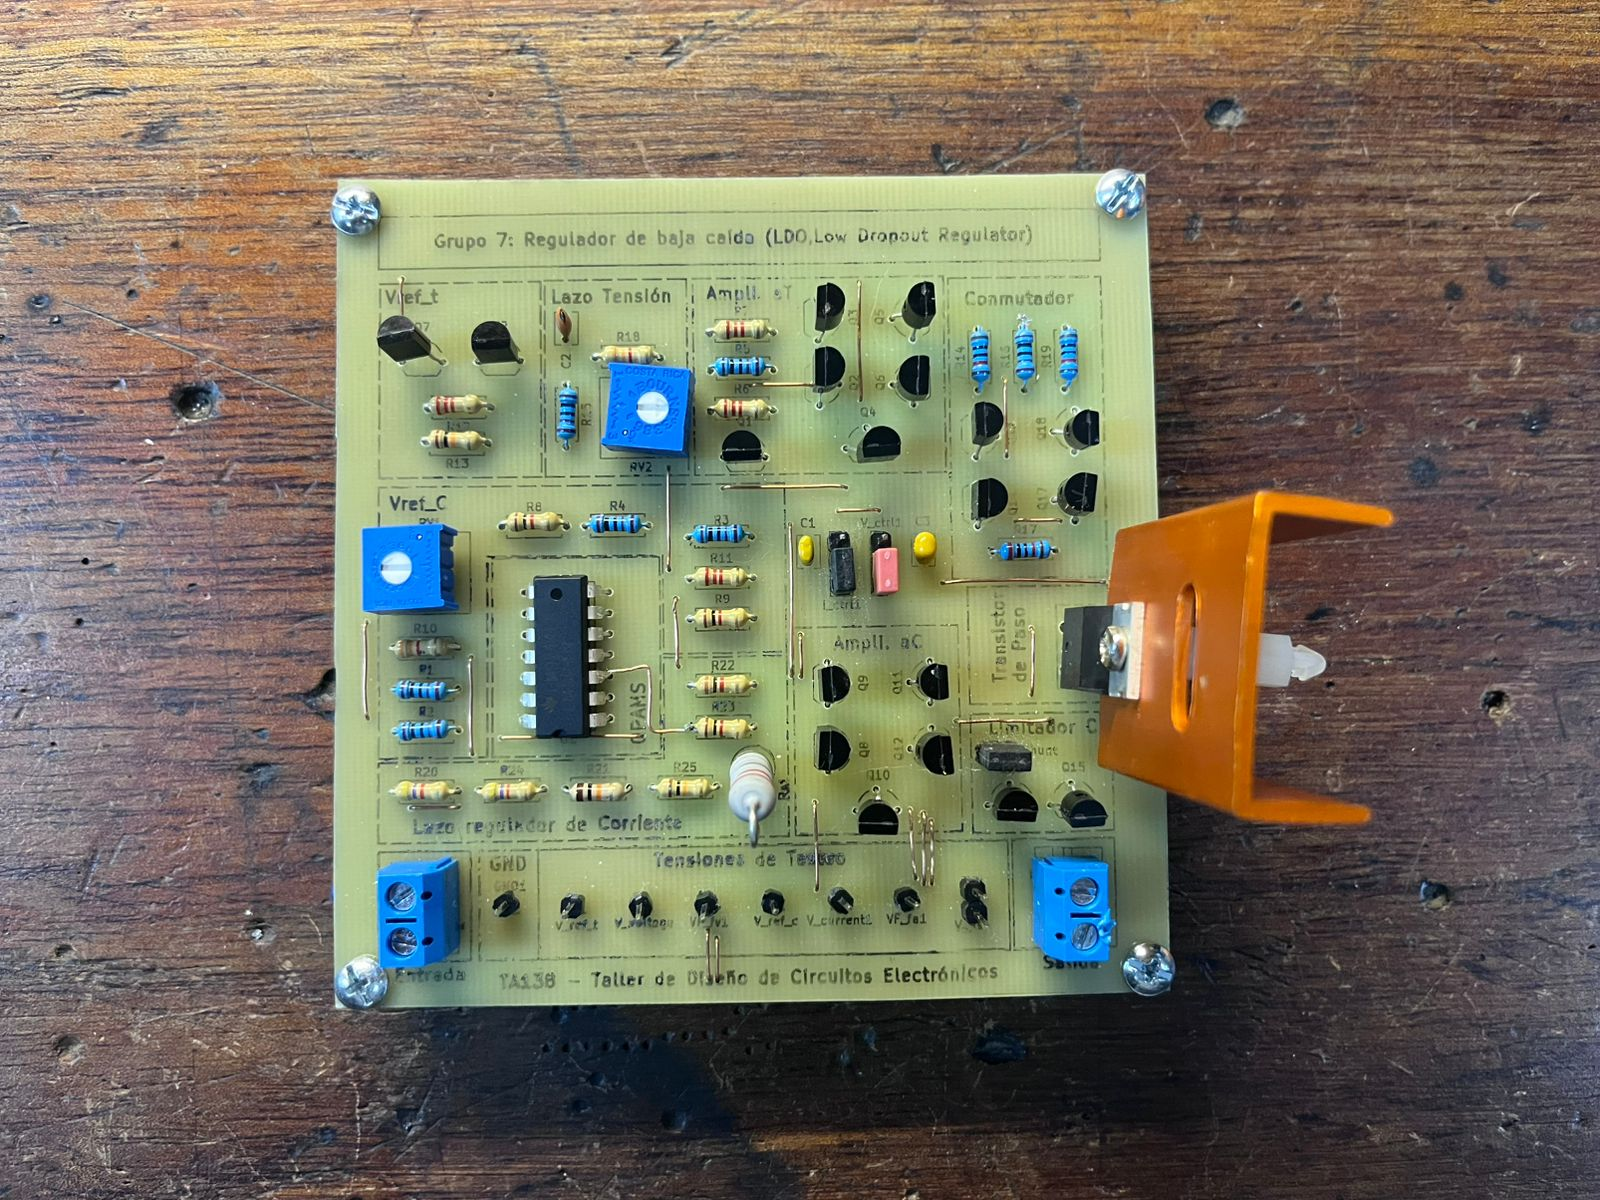
\includegraphics[width=\linewidth]{img/LDO/Placa_montada_1}
			\caption{Placa montada}
		\end{subfigure}
		\hfill
		\begin{subfigure}{0.48\textwidth}
			\centering
			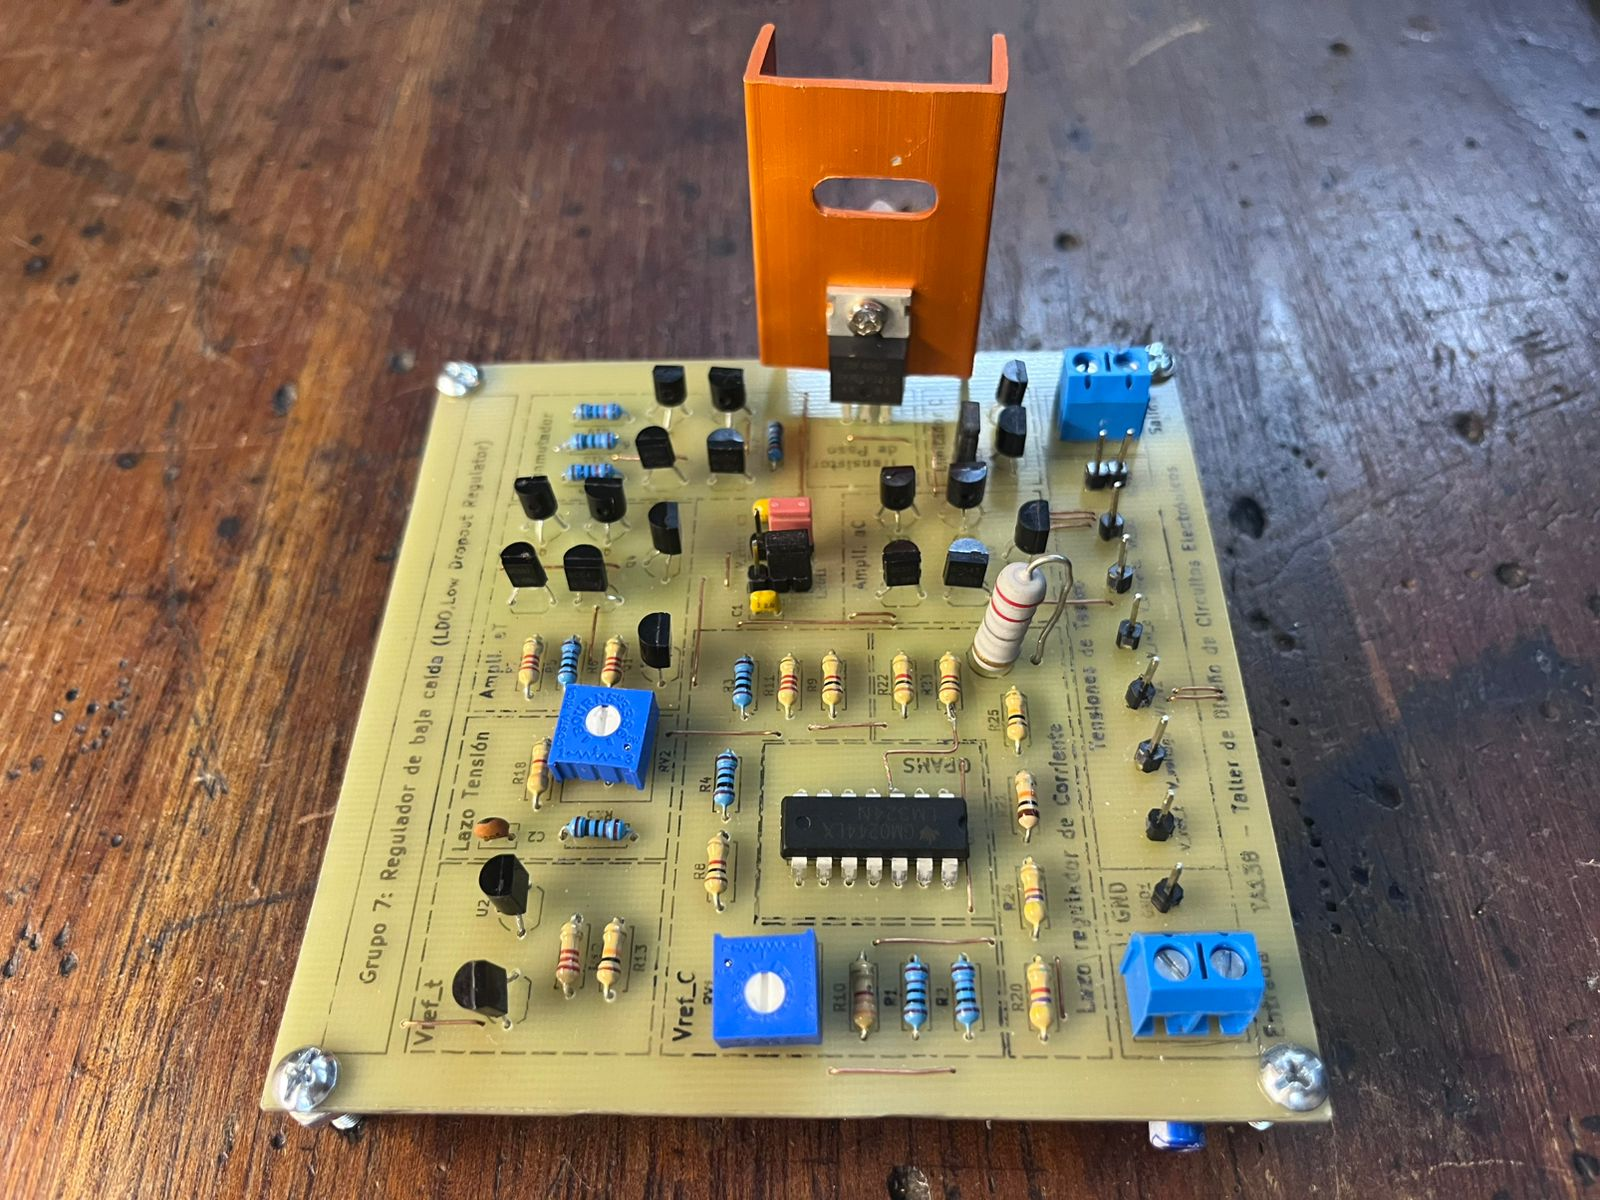
\includegraphics[width=\linewidth]{img/LDO/placa_montada_lateral}
			\caption{Vista lateral}
		\end{subfigure}
		
		\caption{Montaje de la placa LDO}
		\label{fig:placamontada1}
	\end{figure}
	
	
	% SL : voy a seguir la seccion del diseño de pcb a parte y dsp lo añado
	
	\subsubsection{Mejoras:}
	Aunque el regulador lineal satisface las especificaciones de la tabla \ref{tabla:especificaciones_ldo}, hay algunas mejoras que pueden realizarse al circuito para mejorar aun más su desempeño:
	
	\begin{itemize}
		\item \textbf{Mejora de rechazo al ruido:} Se observó que el rechazo al ripple de altas frecuencias (\SI{100}{\kilo\hertz}) no es bueno (ver figura \ref{fig:ldovccvo}). Algunos elementos que favorecen este comportamiento es la alimentación de varios módulos pertenecientes a lazos de realimentación con la fuente de entrada $V_{cc}$. Si se hiciera una relación de compromiso y se limitara $V_{cc max}$, podría alimentarse los lazos con fuentes controladas estables.
		
		Adicionalmente, la tensión de control $V_{gs}$ se ve referida a la fuente de tensión, por lo que, por muy estable que sea $v_g$, seguirá habiendo fluctuaciones. Esta es una limitación importante del transistor de paso canal P. Una forma de contrarestarlo sería hacer la respuesta de los lazos más rápida.
		
		\item \textbf{Lazo de corriente:} El lazo de corriente contiene un máximo de tres etapas amplificadoras, y 5 en total. La implementación más rudimentaria de regulación foldback utiliza tan solo un transistor y tres resistencias. Buscar un modo de reducir la circuitería haría el circuito más rápido, eficiente y simple. Una ventaja de mantener la configuración actual es la precisión de regulación estacionaria.
		
		\item \textbf{Par darlington:} Utilizar un par darlington en los pares diferenciales aumenta enormemente la resistencia $R_{diff}$, así como la ganancia $A_{d}$, por mejorar el valor de $gm$.
	\end{itemize}
	

	
	\section{Simulaciones}
	\label{sec:simulaciones}
	
	\subsection{Simulaciones del regulador lineal LDO}
	\FloatBarrier
	\FloatBarrier
	\subsubsection{Modo estático}
	\FloatBarrier
	
	Para verificar el diseño se realizan simulación en el software LtSpice utilizando los modelos necesarios y las conexiones detalladas en el apéndice \ref{sec:apendice_simulaciónes} en la captura de la figura \ref{fig:ldoregulacionlinea}.
	
	En particular, se evaluaron distintos aspectos fundamentales del desempeño del regulador LDO. En primer lugar, se evaluó la hipótesis $a_o.f \gg 1$ para ambos lazos. Luego se analizó la estabilización de la tensión de salida frente a variaciones temporales de la tensión de entrada y la regulación de línea, que caracteriza la capacidad del regulador para mantener constante la tensión de salida ante cambios en la tensión de entrada. Asimismo, se evaluó la regulación de carga, analizando la variación de la tensión de salida frente a cambios en la corriente demandada por la carga.
	
	Adicionalmente, se calculó la eficiencia del regulador, definida como la relación entre la potencia entregada a la carga y la potencia suministrada por la fuente de entrada. Este análisis permite estimar el rendimiento energético del circuito y las pérdidas asociadas al elemento de paso del regulador.
	
	Se presentan los resultados obtenidos para cada uno de estos casos.
	
	\FloatBarrier
	\paragraph{Ganancias de lazo: }
	\FloatBarrier
	Se observó para ambos lazos que el componente $a_o$ es, escencialmente, el amplificador diferencial al final de cada uno sumado al circuito source común generado por el PMOS. A continuación, se rompe el lazo y se simula la amplitud de salida, del otro lado del lazo, para obtener valor numérico de $|T_t|$ y $|T_c|$.
	
	Para tal efecto, se utiliza una estructura como la de la figura \ref{fig:rompelazo} para conservar el circuito de contínua, pero romper el lazo en señal.
	
	\begin{figure}[h]
		\centering
		\begin{tikzpicture}[transform shape]
			% Paths, nodes and wires:
			\draw (3, 2.75) to[american voltage source, l={$v_p$}] (3, 0.75);
			\draw (5, 4) to[american inductor, mirror, l={$L$}] (3, 4);
			\draw (3, 2.75) to[capacitor, l={$C$}] (3, 4);
			\draw (3, 4) -- (1, 4);
			\node[tlground] at (3, 0.75){};
			\node[circ] at (3, 4){};
			\node[inputarrow, xscale=-1, yscale=-1] at (1, 4){};
			\node[circ](N1) at (5, 4){} node[anchor=west] at (N1.text){$v_o$};
		\end{tikzpicture}
		\caption{Circuito de prueba para cortar lazo.}
		\label{fig:rompelazo}
	\end{figure}
	
	\textbf{Lazo de tensión:}\\
	Se anulan ambos lazos de corriente (shunt y foldback), aunque no se encuentren operativos para la resistencia de carga $R_L = \SI{100}{\ohm}$ elegida, y se coloca la estructura de la figura \ref{fig:rompelazo}. La figura \ref{fig:corte_lazo_tension} muestra el circuito de medición completo.
	
	\begin{figure}[h]
		\centering
		
\includegraphics[width=0.6\linewidth]{img/LDO/Corte_lazo_tension}
		\caption{Circuito utilizado para la medición de $T_v$.}
		\label{fig:corte_lazo_tension}
	\end{figure}
	
	El resultado es un gráfico de Bode como el de la figura \ref{fig:bode_corte_tension}. Que da una ganancia para bajas frecuencias $T_v = \SI{86}{dB}$. Esto es suficiente para asegurar $a_o.f_v \gg 1$.
	
	\begin{figure}[h]
		\centering
		\includegraphics[width=0.85\linewidth]{"../../Simulación/LDO/Graficos en Python/Capturas/LDO_Bode_lazo_tension"}
		\caption{Bode resultante de la medición de $T_v$. Notar el polo en $f \sim \SI{10}{k\ohm}$.}
		\label{fig:bode_corte_tension}
	\end{figure}
	
	En este gráfico queda en evidencia el por qué de la oscilación para la regulación de línea (\ref{fig:ldovccvo}), pues la frecuencia de ruido $\sim \SI{100}{k\hertz}$ seguramente se encuentre en un punto con ganancia $|T| > 1$ y fase negativa, produciendo realimentación positiva y oscilaciones.
	
	A continuación se varía la resistencia de carga para buscar el caso más descompensado. Dadas las resistencias $R_3$ y $R_4$, se espera que el peor caso se encuentre en resistencias de carga $R_L \gg R_3 // R_4$. La figura \ref{fig:bode_corte_tension2} muestra el resultado de la simulación.
	
	\begin{figure}
		\centering
		\includegraphics[width=0.85\linewidth]{"../../Simulación/LDO/Graficos en Python/Capturas/LDO_Bode_lazo_tension_comparacion"}
		\caption{Bode resultante de la medición de $T_v$ para diferentes valores de $R_L$.}
		\label{fig:bode_corte_tension2}
	\end{figure}
	
	Una vez compensado el lazo, según se analiza en la sección \ref{sec:compensacion}:Lazo de tensión, el gráfico de bode tendrá la forma de la figura \ref{fig:bode_tension_compensado}.
	
	\begin{figure}[h]
		\centering
		\includegraphics[width=0.85\linewidth]{"../../Simulación/LDO/Graficos en Python/Capturas/LDO_Bode_lazo_tension_compensado"}
		\caption{Bode resultante de la medición de $T_v$ para un lazo de tensión compensado con diferentes cargas.}
		\label{fig:bode_tension_compensado}
	\end{figure}
	
	\textbf{Lazo de corriente:}\\
	En este caso, se realiza el procedimiento inverso. Se anula el lazo de tensión y shunt, y se corta el lazo de corriente en un punto de alta impedancia, como la base del transistor de paso. En la figura \ref{fig:corte_lazo_corriente} puede verse el circuito de medición completo.
	
	\begin{figure}[h]
		\centering
		
\includegraphics[width=0.6\linewidth]{img/LDO/Corte_lazo_corriente}
		\caption{Circuito utilizado para la medición de $T_A$.}
		\label{fig:corte_lazo_corriente}
	\end{figure}
	
	El resultado es un gráfico de Bode como el de la figura \ref{fig:bode_corte_corriente}. Que da una ganancia para bajas frecuencias $T_A = \SI{67}{dB}$. Esto es suficiente para asegurar $a_o.f_A \gg 1$.
	
	\begin{figure}[h]
		\centering
		\includegraphics[width=0.85\linewidth]{"../../Simulación/LDO/Graficos en Python/Capturas/LDO_Bode_lazo_corriente_comparacion"}
		\caption{Bode resultante de la medición de $T_A$ para diferentes valores de $R_L$.}
		\label{fig:bode_corte_corriente}
	\end{figure}
	
	Finalmente, se simula simula bajo las mismas condiciones el lazo de corriente compensado. El resultado puede verse en la figura \ref{fig:bode_corriente_compensado}.
	
		\begin{figure}[h]
		\centering
		\includegraphics[width=0.85\linewidth]{"../../Simulación/LDO/Graficos en Python/Capturas/LDO_Bode_lazo_corriente_compensado"}
		\caption{Bode resultante de la medición de $T_A$ para el lazo de corriente compensado.}
		\label{fig:bode_corriente_compensado}
	\end{figure}
	\FloatBarrier
	\paragraph{Estabilización de tensión: }
	\FloatBarrier
	En la simulación temporal se verifica la estabilización de tensión con respecto a la $Vcc$ prevista, utilizando un valor de carga dentro de la zona de regulación estimada, logrando así constatar cómo se reduce el ripple. Se simula tomando un valor de carga dentro del rango de regulación, y se toman los valores de tensión en función del tiempo, para el análisis se comparan las componentes alternas de cada señal eliminando el valor medio de ambas, tal como se observa en los gráficos de la figura \ref{fig:ldovccvo}.
	
	Notar que la compensación favorece el rechazo al ruido de entrada, al mismo tiempo que evita la oscilación del ciruito.
	
	\begin{figure}[h]
		\centering
		\begin{subfigure}[b]{0.55\linewidth}
		\includegraphics[width =\linewidth]{"../../Simulación/LDO/Graficos en Python/Capturas/LDO_Vcc_Vo"}
		\caption{Caso descompensado.}
		\end{subfigure}
		\hfill
		\begin{subfigure}[b]{0.55\linewidth}
		\includegraphics[width = \linewidth]{"../../Simulación/LDO/Graficos en Python/Capturas/LDO_Vcc_Vo_compensado"}
		\caption{Caso compensado.}
	\end{subfigure}
		\caption{Gráfico de la simulación temporal con ruido a la entrada $V_{pp} = \SI{0.4}{V} , f = \SI{100}{\kilo H}$.}
		\label{fig:ldovccvo}
	\end{figure}
	
	
	\FloatBarrier
	\paragraph{Regulación de Linea:}
	\FloatBarrier
	
	La regulación de línea describe la capacidad del regulador para mantener constante la tensión de salida frente a variaciones en la tensión de entrada \(V_{CC}\).
	
	Para caracterizar este comportamiento, se realiza un barrido de la tensión de entrada y se gráfica la tensión de salida \(V_O\) en función de \(V_{CC}\), para una carga fija de $R_L = \SI{10}{\kilo\ohm}$.
	
	\begin{itemize}
		\item \textbf{Zona de regulación:}  
		Para valores suficientemente altos de \(V_{CC}\), el regulador opera en condiciones normales y la tensión de salida permanece aproximadamente constante e igual al valor nominal. En esta región, el lazo de realimentación compensa las variaciones de entrada.
		
		\item \textbf{Zona de dropout:}  
		A medida que \(V_{CC}\) disminuye, se alcanza un punto en el cual el regulador no puede mantener la tensión de salida constante. Esto ocurre cuando el transistor de paso entra en saturación (o pierde margen de control), y la salida comienza a seguir a la entrada.
		
		\item \textbf{Transición:}  
		El punto de transición entre ambas regiones indica el inicio de la condición de dropout.
	\end{itemize}
	
	A partir de esta curva, es posible estimar la tensión de dropout como la diferencia entre la tensión de entrada y la tensión de salida en el punto donde el regulador deja de mantener la regulación:
	
	\[
	V_{dropout} = V_{{CC}_{min}} - V_O \approx \SI{320}{mV}
	\]
	
	En consecuencia, la curva de regulación de línea no sólo permite evaluar la estabilidad de la salida frente a perturbaciones en la entrada, sino también identificar el margen mínimo de operación del regulador.
	
	En la figura \ref{fig:ldoregulacionlinea} puede verse la curva de salida en función de la entrada para $\SI{0}{V} < V_{cc} < \SI{24}{V}$ y en mayor precisión la zona de Dropout. De la simulación se obtiene
	
	\begin{equation}
		Regulacion \ de \ Linea = \num{447.68} \frac{\si{\micro V}}{\si{V}},
	\end{equation}
	
	con un pequeño offset $V_{offset} = \SI{90}{mV}$, resultante de $V_ref-t = \SI{1.242}{V} \ne \SI{1.25}{V}$, fácilmente corregible mediante el preset implementado.
	
	Además, se ve que la tensión de dropout tiene valor $\SI{100}{mV} < V_{DO} < \SI{320}{mV}$, con su valor máximo alcanzado cuando $V_{cc} = \SI{5.27}{V}$. (Esto ocurre porque, debido al offset de $v_{ref-t}$, el valor de regulación no es \SI{5}{V} exactamente).
	
	\begin{figure}[h]
		\centering
		\begin{subfigure}{0.45\linewidth}
			\includegraphics[width=\linewidth]{"../../Simulación/LDO/Graficos en Python/Capturas/LDO_regulacion_linea"}
			\caption{Regulación de línea para $\SI{0}{V} < V_{cc} < \SI{24}{V}$.}
		\end{subfigure}
		\hfill
		\begin{subfigure}{0.45\linewidth}
			\includegraphics[width=\linewidth]{"../../Simulación/LDO/Graficos en Python/Capturas/LDO_regulacion_linea_zoom"}
			\caption{Zoom para $\SI{3.5}{V} < V_{cc} < \SI{5.5}{V}$.}
		\end{subfigure}
		
		\caption{Gráfico de los datos de simulación de línea.}
		\label{fig:ldoregulacionlinea}
	\end{figure}
	
	
	\FloatBarrier
	\paragraph{Regulación de carga:}
	\FloatBarrier
	La regulación de carga puede analizarse evaluando la variación de la tensión de salida \(V_O\) frente a cambios en la resistencia de carga \(R_L\). Esto se analiza insertando una fuente de corriente a la salida, para una $V_{cc} = \SI{9.5}{V}$ constante, y desconectando el lazo de corriente.
	
	Para ello, se realiza un barrido del valor de \(R_L\) y se observa la respuesta del regulador.
	
	\begin{itemize}
		\item \textbf{Altos valores de \(R_L\):}  
		Corresponden a condiciones de baja corriente de carga. En esta región, el regulador mantiene la tensión de salida cercana a su valor nominal.
		
		\item \textbf{Disminución de \(R_L\):}  
		A medida que la resistencia de carga disminuye, la corriente demandada aumenta. Idealmente, el regulador debería mantener \(V_O\) constante.
		
		\item \textbf{Comportamiento real:}  
		En la práctica, se observa una leve caída de la tensión de salida debido a la resistencia de salida finita del regulador y a las limitaciones del transistor de paso.
	\end{itemize}
	
	Este análisis permite evaluar la capacidad del regulador para sostener la tensión de salida frente a variaciones en la carga, aunque resulta menos directo que el análisis en función de la corriente.
	
	En la figura \ref{fig:ldoregulacioncarga} puede verse la gráfica resultante. Notar que, al poseer un lazo de corriente shunt aún activo, modificar la corriente de entrada directamente provoca una abrupta caída de tensión para $I_o > \SI{2.25}{A}$. Aun así, para la zona de control propia del lazo de tensión, pueden obtenerse resultados:
	
	\begin{equation}
		\frac{\Delta V}{\Delta I} = -1,36 \frac{\si{mV}}{\si{A}} = R_T
	\end{equation}
	
	Notar que $R_T$ es negativa por disminuir $V_o$ al aumentar $I_o$.
	
	\begin{figure}[h]
		\centering
		\includegraphics[width=0.60\linewidth]{"../../Simulación/LDO/Graficos en Python/Capturas/LDO_regulacion_carga"}
		\caption{Regulación de carga del regulador lineal.}
		\label{fig:ldoregulacioncarga}
	\end{figure}
	
	\FloatBarrier
	\paragraph{$V_o$ en función de $I_L$:}
	\FloatBarrier
	Este gráfico muestra de forma cualitativa la curva característica de la fuente de tensión resultante, es decir, la gráfica $V_o/I_L$ (figura \ref{fig:VvsI}), mediante la variación del valor resistivo de la carga $R_L$.
	
	Se observa que la tensión es constante para valores $R_L > \SI{3.3}{\ohm}$, y al cortocircuitar más la carga comienza a caer hacia $V_o = \SI{0}{V}$, siguiendo la curva de corriente $I_o = 400mA + \frac{\SI{1.1}{A}}{\SI{5}{V}} \cdot V_o$.
	
	\begin{figure}[h]
		\centering
		\includegraphics[width=0.6\linewidth]{"../../Simulación/LDO/Graficos en Python/Capturas/V vs I"}
		\caption{Curva de salida característica estática regulador LDO.}
		\label{fig:VvsI}
	\end{figure}
	
	\FloatBarrier
	\paragraph{Eficiencia:}
	\FloatBarrier
	Para medir la eficiencia del circuito, se ingresan diferentes valores de tensión de entrada $V_{cc}$ y se evalúa la potencia de entregada y la potencia sobre la carga, para una $R_L = \SI{100}{\ohm}$. El resultado se observa en la figuar \ref{fig:ldoeficiencia}.
	
	Como es de esperar para un regulador lineal, la eficiencia no es buena, y es fuertemente dependiente de la tensión de entrada. Esto se debe a que el transistor de paso disipa la potencia no útil:
	
	\begin{equation}
		P_{Tpaso} = (V_{cc} - V_{reg}) * (V_{reg}/R_L)
	\end{equation}
	
	Como tal, se espera una eficiencia máxima para valores $V_{cc}$ cercanos a $V_{reg}$ y resistencias de carga $R_L$ bajas. Al aumentar $R_L$, la eficiencia aumenta hasta el punto donde la corriente que circula por el circuito de control se hace comparable con la que circula por $R_L$.
	
	\begin{figure}[h]
		\centering
		\includegraphics[width=0.7\linewidth]{"../../Simulación/LDO/Graficos en Python/Capturas/LDO_eficiencia"}
		\caption{Eficiencia del regulador para $\SI{0}{V} < V_{cc} < \SI{24}{V}$.}
		\label{fig:ldoeficiencia}
	\end{figure}
	
	\FloatBarrier
	\subsubsection{Modo Dinámico}
	\FloatBarrier
	Se evalúa el comportamiento en modo dinámico de ambos lazos de realimentación. El objetivo es corroborar la compensación y observar el tiempo de respuesta de cada uno. Para ello, se debe variar la carga de forma abrupta, provocando una respuesta al escalón.
	
	Dicho comportamiento se logra con el componente Switch, controlado por una fuente de tensión(figura \ref{fig:carga_activa}). Luego se observa tensión resultante a la salida.
	
	\begin{figure}[h]
		\centering
		
\includegraphics[width=0.3\linewidth]{img/LDO/Carga_activa}
		\caption{Circuito de testeo dinámico utilizado como carga activa.}
		\label{fig:carga_activa}
	\end{figure}
	
	Para el lazo de tensión, se utiliza 
	
	$$(R_{20} = \SI{100}{\kilo\ohm},R_{21} = \SI{1}{\kilo\ohm})\to R_{L1} = \SI{100}{\kilo\ohm},R_{L2} = \SI{1}{\kilo\ohm}$$
	
	Para el lazo de corriente, se buscará un valor de $0 < R_L < \SI{3.3}{\ohm}$ tal que el lazo de corriente se encuentre activo. En este caso
	
	$$(R_{20} = \SI{2.5}{\ohm},R_{21} = \SI{1.5}{\ohm}) \to R_{L1} = \SI{2.5}{\ohm},R_{L2} = \SI{1}{\ohm}$$
	
	Los resultados se ven en la figura \ref{fig:simulacion_dinamica}. Notar que la respuesta para el lazo de corriente no tiende al mismo valor de tensión ni corriente, por tratarse de regulación tipo foldback.
	
	\begin{figure}
		\centering
		\includegraphics[width=0.85\linewidth]{"../../Simulación/LDO/Graficos en Python/Capturas/LDO_lazos_dinamicos"}
		\caption{Respuesta dinámica del regulador LDO.}
		\label{fig:simulacion_dinamica}
	\end{figure}
	
	El lazo de tensión exhibe una respuesta de duración aproximada \SI{5}{\micro s}, con una excursión mínima. El lazo de corriente, sin embargo, es más lento, con una duración de respuesta dinámica de \SI{25}{\micro s}, con tiempos de asentamiento variables.
	
	 De la observación de la figura \ref{fig:bode_corriente_compensado}, se observa que el desplazamiento del polo asociado al nodo gate ocasiona un margen de fase dependiente de la resistencia de carga, volviendo el lazo progresivamente inestable hacia $R_L \to \infty$. En nuestro caso, y debido al acotado rango de operación del lazo de corriente, no será necesario tener en cuenta este fenómeno. En la práctica, si el margen de fase se achicara demasiado, bastará con incrementar el capacitor de compensación, a costa de la velocidad de respuesta.
	
	Es de especial importancia el sobrepico de corriente ocasionado por el abrupto cambio de carga. Notar que, si bien será limitado por el regulador de tipo shunt, deberá ser tenido en cuenta a la hora de conectar una carga. La duración del mismo es de \SI{2.5}{\micro\second}.

	\FloatBarrier
	\subsection{Simulaciones de fuente switching}
	\FloatBarrier
	\subsubsection{fuente \textit{buck} a lazo abierto}
	
	
	Se simuló mediante el software Ltspice el comportamiento del circuito utilizando el esquematico de la captura \ref{fig:simulacionbucklazoabierto} y los diferentes modelos de componentes a lazo abierto, es decir sin utilizar la realimentación para el control de los transistores si no un generador de pruebas en el transistor que implementaría el $t_{on}$ y un diodo de rapida conmutación en reemplazo del transistor de tiempo $t_{off}$ . 
	
	\begin{figure}[H]
		\centering
		
\includegraphics[width=0.7\linewidth]{img/buck/simulacion_buck_lazo_abierto2}
		\caption{Captura esquemático de simulación en ltspice de circuito \textit{buck} a lazo abierto.}
		\label{fig:simulacionbucklazoabierto}
	\end{figure}
	
	
	Se puede verificar la correcta regulación luego de un transitorio, graficando los datos de tensión de salida extraidos de la simulación como se muestra en la Fig. \ref{fig:reguladorbucklazoabierto}.
	
	
	\begin{figure}[H]
		\centering
		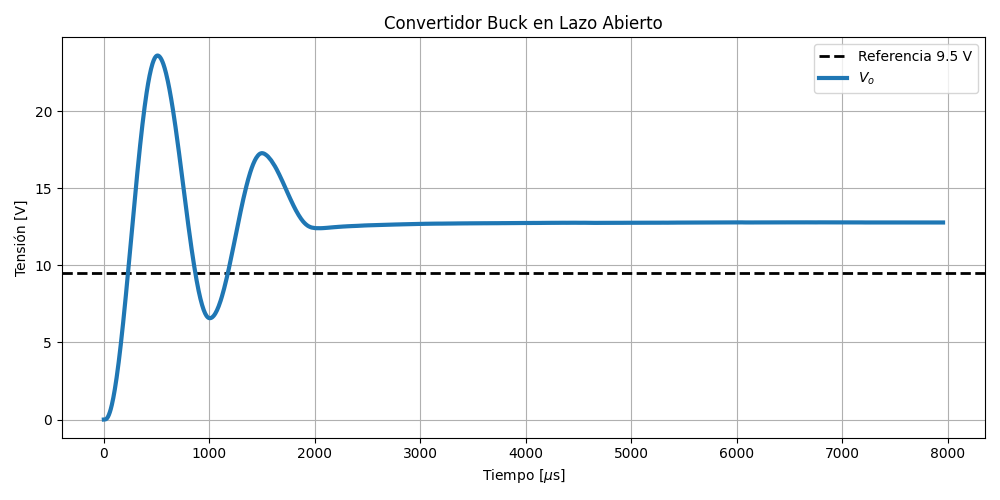
\includegraphics[width=0.7\linewidth]{../../Simulación/BUCK/Datos/regulador_buck_Lazo_abierto2}
		\caption{Datos de tensión de salida extraídos de la simulación del \textit{buck} a lazo abierto.}
		\label{fig:reguladorbucklazoabierto}
	\end{figure}
	
	
	Mientras que en la Fig. \ref{fig:corrientesiliobucklazoabierto} se verifica que se encuentra trabajando en conducción continua.
	
	\begin{figure}[H]
		\centering
		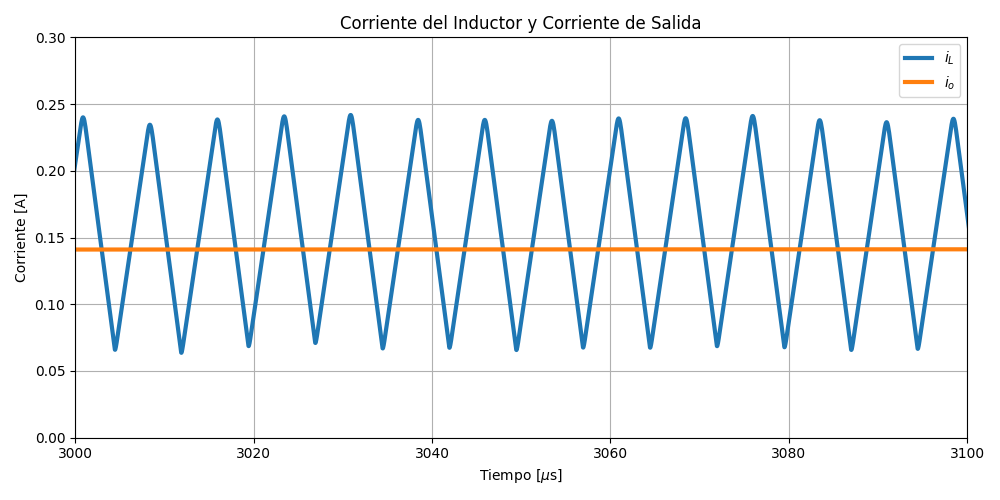
\includegraphics[width=0.7\linewidth]{../../Simulación/BUCK/Datos/corrientes}
		\caption{Corriente en el inductor y resistor de salida, datos extraídos de la simulación del \textit{buck} a lazo abierto.}
		\label{fig:corrientesiliobucklazoabierto}
	\end{figure}
	\subsubsection{PWM}
	
	Se realizan diferentes simulaciones sobre el archivo de la figura \ref{fig:esquematicobuckpwm}. Será de interés la triangular resultante, la señal pwm generada y su interacción con el valor medido. Para la medición a lazo abierto, se simula una entrada senoidal de valor medio \SI{9.5}{V}, con una amplitud de \SI{1.5}{V}.
	
	La señal triangular resultante puede verse en la figura \ref{fig:sim_triag}, y su interacción con la señal de salida PWM puede verse en la figura \ref{fig:sim_pwm2}.
	
	\begin{figure}[H]
		\centering
		\includegraphics[width=0.7\linewidth]{../../Simulación/BUCK/Datos/grafico_pwm}
		\caption{Señal triangular simulada.}
		\label{fig:sim_triag}
	\end{figure}
	
	\begin{figure}[H]
		\centering
		\includegraphics[width=0.7\linewidth]{../../Simulación/BUCK/Datos/grafico_pwm2}
		\caption{Señal PWM resultante.}
		\label{fig:sim_pwm2}
	\end{figure}
	
	Se observa que el comportamiento es coherente con los resultados calculados, con la salvedad de la frecuencia de oscilación, que es un poco más alta $f_s = \SI{128}{\kilo\hertz}$.
	
	
	
	\section{Mediciones}
	\subsection{LDO}
	
	Con el objetivo de validar experimentalmente el desempeño del regulador implementado, se llevaron a cabo una serie de mediciones sobre el prototipo construido. Estas pruebas permiten contrastar los resultados obtenidos en la etapa de diseño y simulación con el comportamiento real del circuito, evaluando parámetros clave como la regulación de carga, la regulación de línea, la capacidad de limitación de corriente y la eficiencia del sistema. A continuación, se describe el banco de pruebas utilizado y la metodología empleada en cada caso.
	
	\subsubsection{Banco de Pruebas}
	
	Para realizar las mediciones se llevo la placa a el laboratorio y se la dispuso frente a un banco de pruebas compuesto por los siguientes instrumentos de medición.
	
	%completar al medir
	\begin{itemize}
		\item Fuente : UNI-T, UTP33115TFL-II
		\item Generador de Señales, Topware, 8105  
		\item Osciloscopio : UNI-T, UTD2102CEX+
		\item Multimetro: VT-POWER, M890G
		\item Banco de baterías
	\end{itemize}
	
	\begin{figure}[H]
		\centering
		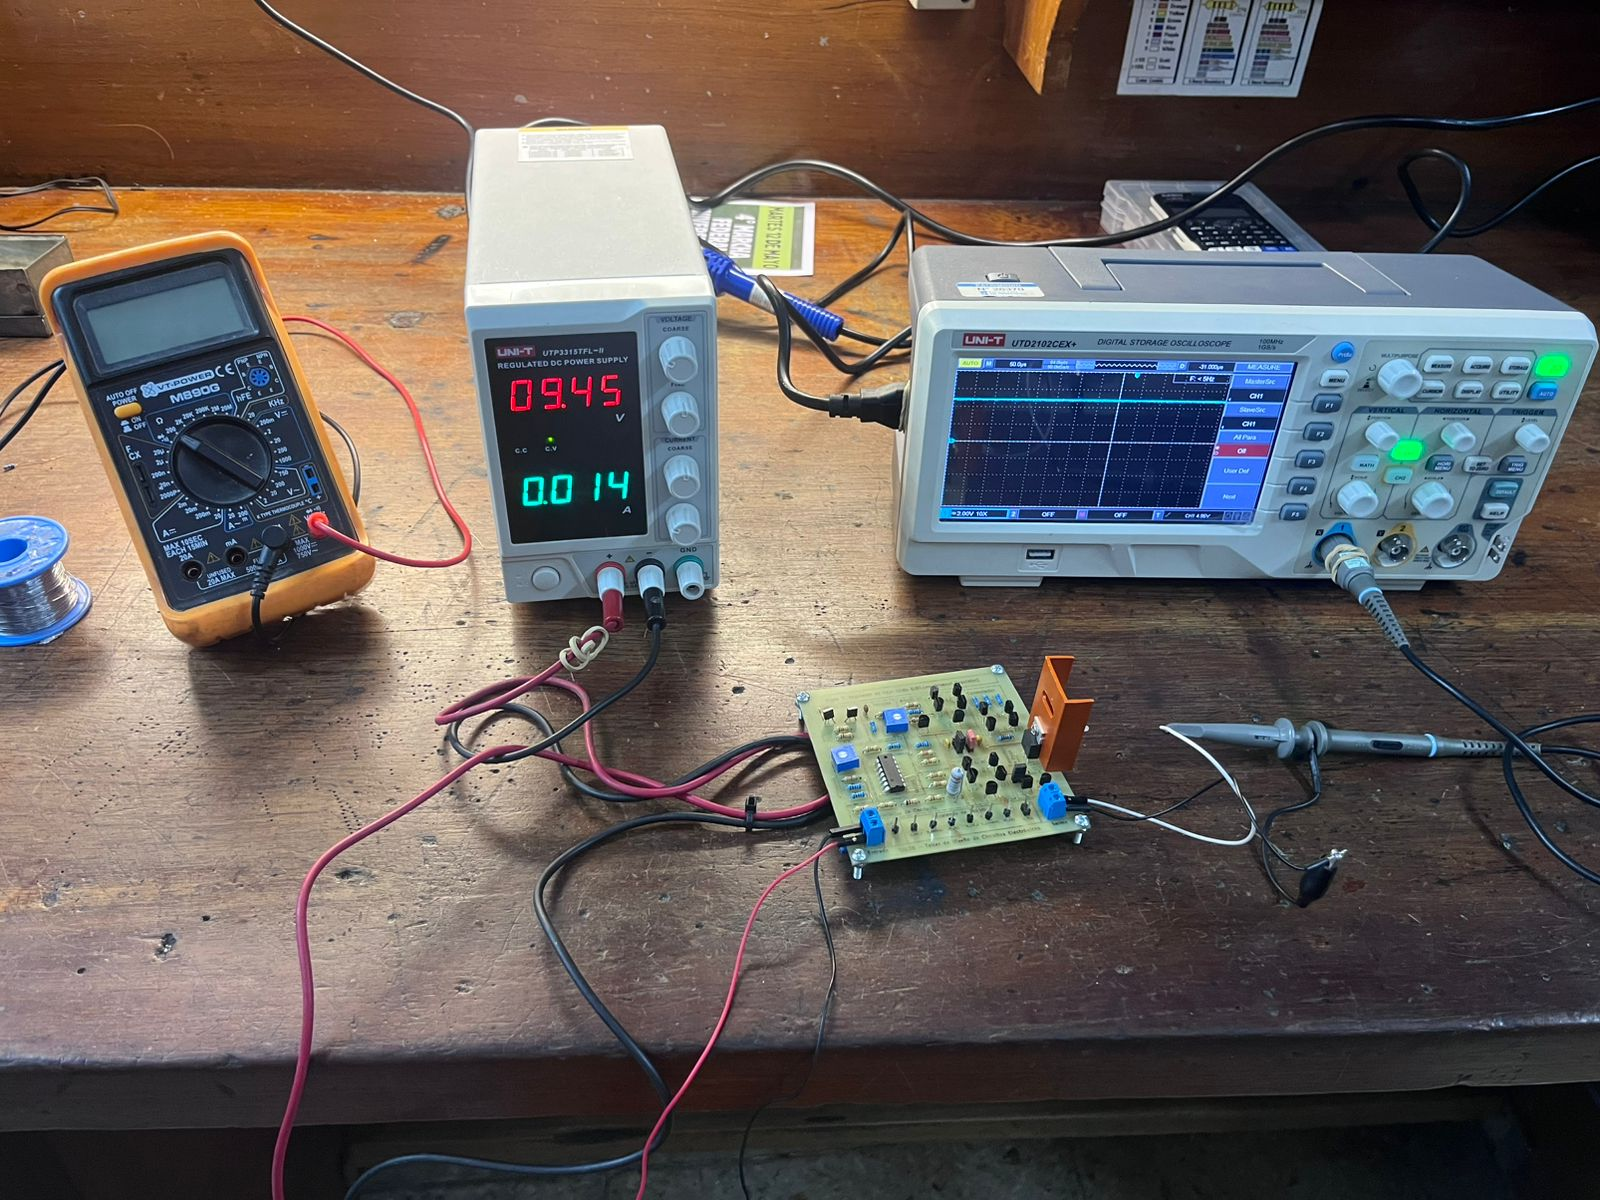
\includegraphics[width=0.8\linewidth]{img/LDO/banco_medicion}
		\caption{banco de medición en laboratorio.}
		\label{fig:bancomedicion}
	\end{figure}
	
	
	\begin{figure}[H]
		\centering
		
		% =========================
		% IMAGEN 1 (batería)
		% =========================
		\begin{minipage}{0.25\textwidth}
			\centering
			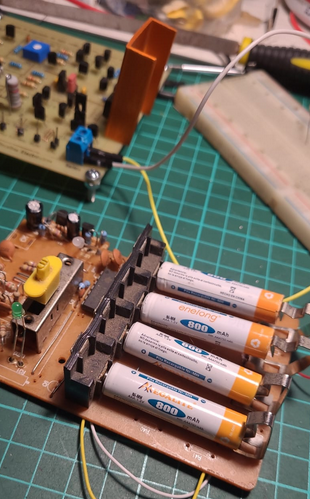
\includegraphics[width=\linewidth]{img/LDO/bateria_p_medir}
			\caption{Banco de baterías para obtener tensión de referencia de bajo ruido.}
			\label{fig:bateriapmedir}
		\end{minipage}
		\hfill
		% =========================
		% IMAGEN 2 (generador)
		% =========================
		\begin{minipage}{0.62\textwidth}
			\centering
			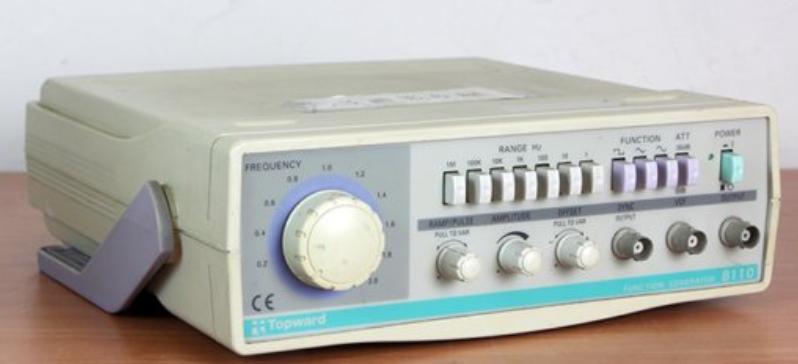
\includegraphics[width=\linewidth]{img/LDO/generador_señales}
			\caption{Modelo de generador de señales utilizado en las pruebas.}
			\label{fig:generadorsenales}
		\end{minipage}
		
	\end{figure}
	
	\subsubsection{Regulación de carga estática y dinámica}
	\label{sec:regulacion}
	
	La regulación idealmente no debe depender del tipo de carga, sin embargo una carga de poca resistencia consume mucha corriente que la fuente debe ser capaz de entregar y una carga que varié su resistencia infiere que la fuente debe cambiar su estado de equilibrio rápidamente a uno nuevo, esto previamente se a simulado, y en las próximas mediciones se verificara y se caracterizara el circuito de forma practica con componentes reales.
	
	\paragraph{Regulación de carga estática }\hfill\break
	
	Para la regulación de carga se varia la resistencia de carga desde valores grandes de resistencias hacia los puntos críticos donde la corriente llega a su limite y debe actuar la regulación de corriente. Dichos valores medidos se encuentran tabulados en la tabla \ref{tab:reg_carga_ldo} y la curva obtenida tras interpolar los puntos medidos en la figura \ref{fig:regulacioncarga}. A su vez se realizo el calculo de resistencia de Thevenin correspondiente a la caracterización de la resistencia de salida del regulador lineal.
	
	En búsqueda de una mayor sensibilidad de medición se midió la diferencia de la tensión de salida con respecto una fuente fija de tensión de $5,22 \,V$ tal como se detalla en el diagrama de la figura \ref{fig:medicionregcargabanco}, luego dicha diferencia ,en el orden de los mV, fue la variación que afecto cada punto de medición.
	\begin{figure}[H]
		\centering
		
		% =========================
		% IZQUIERDA: IMAGEN
		% =========================
		\begin{minipage}{0.55\textwidth}
			\centering
			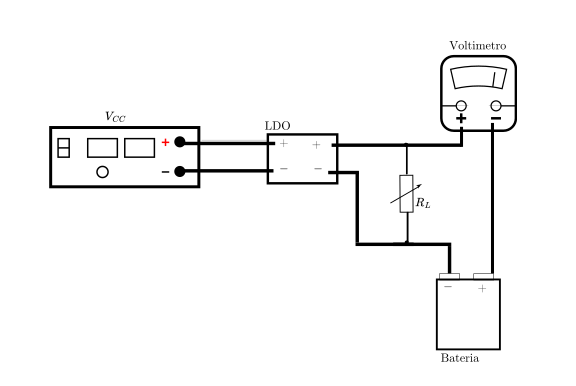
\includegraphics[width=\linewidth]{img/LDO/Diagramas medicion/medicion_reg_carga_banco.png}
			\caption{Banco de pruebas para medición de regulación de carga}
			\label{fig:medicionregcargabanco}
		\end{minipage}
		\hfill
		% =========================
		% DERECHA: TABLA
		% =========================
		\begin{minipage}{0.42\textwidth}
			\centering
			\captionof{table}{Mediciones de regulación de carga estática del LDO}
			\label{tab:reg_carga_ldo}
			\begin{tabular}{|c|c|}
				\hline
				\textbf{$R_L$ [$\Omega$]} &
				\textbf{$V_O$ [V]} \\
				\hline
				100k & 4.8186 \\
				10k  & 4.8079 \\
				4k7  & 4.8071 \\
				1k   & 4.8038 \\
				560  & 4.8025 \\
				220  & 4.7950 \\
				100  & 4.7830 \\
				47   & 4.7630 \\
				23.5 & 4.7650 \\
				10   & 4.6270 \\
				\hline
			\end{tabular}
		\end{minipage}
		
	\end{figure}
	
	\begin{figure}[H]
		\centering
		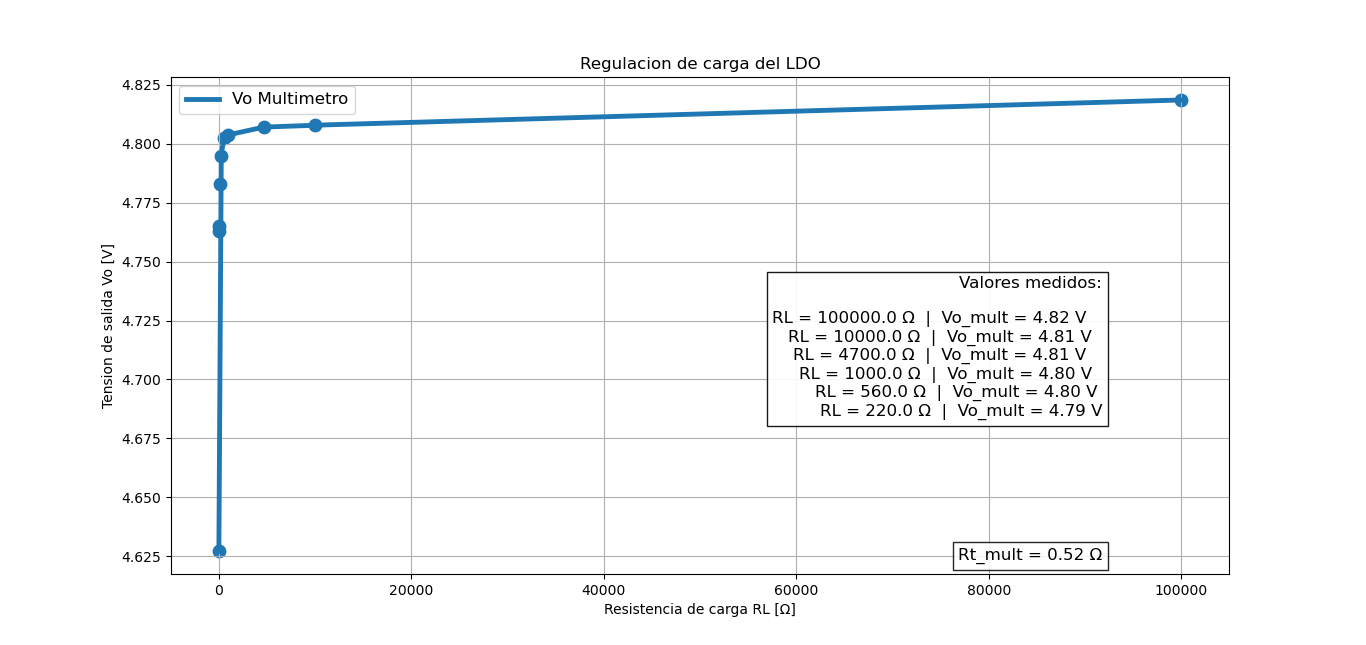
\includegraphics[width=1\linewidth]{../Graficos/regulacion_carga}
		\caption{Interpolación de los puntos medidos en regulación de carga estática.}
		\label{fig:regulacioncarga}
	\end{figure}
	
	Tomando dos puntos de la curva correspondientes a la resistencia de $1 \, k\Omega$  y de $220 \, \Omega$ y utilizando la expresión \ref{eq:rt_general} se llega a el valor de resistencia de salida de $0,52 \Omega$.
	
	\begin{equation} 
		R_T =
		\frac{
			\left(
			1-\dfrac{V_1}{V_2}
			\right)R_2
		}{
			\left(
			\dfrac{V_1}{V_2}\cdot\dfrac{R_2}{R_1}
			\right)-1
		} = 0,52 \, \Omega
		\label{eq:rt_general}
	\end{equation}
	
	
	\paragraph{Regulación de carga dinámica}\hfill\break
	
	Para una carga dinámica se debe considerar una carga activa que varié su corriente, se medirá utilizando como carga una fuente de corriente con un transistor. El regulador deberá mantener la tensión de salida con una variación acotada en
	función de la variación de la corriente en la carga.
	
	\begin{figure}[H]
		\centering
		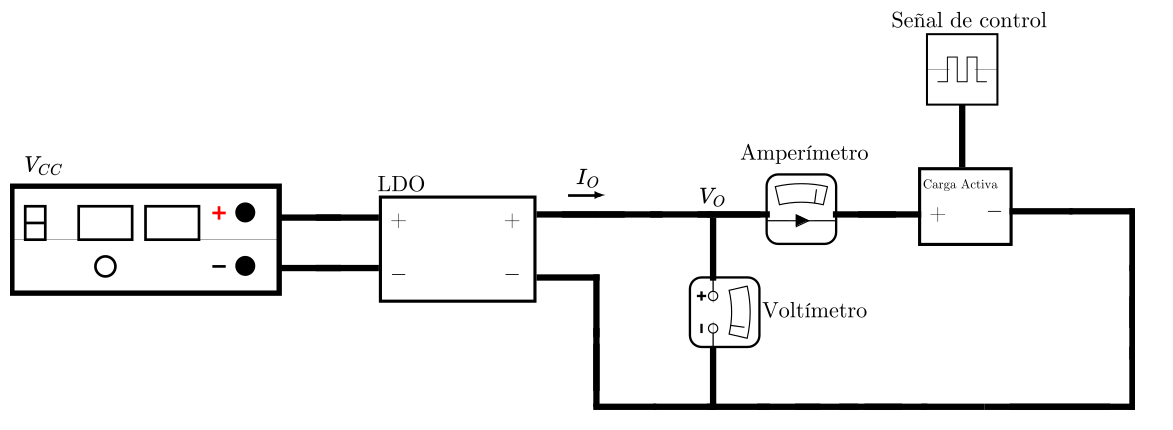
\includegraphics[width=1\linewidth]{img/LDO/Diagramas medicion/carga_activa}
		\caption{Disposición del banco de medición para carga activa.}
		\label{fig:cargaactiva}
	\end{figure}
	\begin{figure}[H]
		\centering
		\begin{minipage}{0.45\textwidth}
			\centering
			
			\begin{tikzpicture}[transform shape, scale=1.2]
				% Paths, nodes and wires:
				\node[npn] at (33, 5){};
				\draw (33, 4.25) to[american resistor, /tikz/circuitikz/bipoles/length=1.09cm, l={$R_E$}] (33, 2.5);
				\node[sground] at (33, 2.5){};
				\node[sground] at (30.98, 3.34){};
				
				\node[shape=rectangle, minimum width=1.215cm, minimum height=0.215cm] 
				at (33.25, 7){}
				node[anchor=north west, align=left, text width=0.827cm, inner sep=6pt] 
				at (32.625, 7.125){$V_o$};
				
				\node[circ] at (33, 6.5){};
				\draw (33, 5.75) -- (33, 6.5);
				
				\node[shape=rectangle, minimum width=4.84cm, minimum height=0.84cm] 
				at (33.71, 4.118){}
				node[anchor=north west, align=left, text width=4.452cm, inner sep=6pt] 
				at (31.272, 4.555){\tiny Generador de\\funciones};
				
				\draw[-latex] (33.25, 5.812) -- (33.25, 5.375);
				
				\node[shape=rectangle, minimum width=1.215cm, minimum height=0.215cm] 
				at (33.875, 5.75){}
				node[anchor=north west, align=left, text width=0.827cm, inner sep=6pt] 
				at (33.25, 5.875){$i_o$};
				
				\draw (31, 4.75) to[square voltage source, mirror] (30.98, 3.34);
				\draw (32.16, 5) -- (31, 5) -- (31, 4.75);
			\end{tikzpicture}
			
		\end{minipage}
		\hfill
		\begin{minipage}{0.53\textwidth}
			
			Se implementó una carga dinámica basada en un transistor NPN controlado mediante un generador de funciones configurado con una señal cuadrada de 1 kHz y 2 V pico. El colector del transistor se conecta a la salida del regulador, mientras que el emisor posee una resistencia $R_E$ de 1k hacia referencia, permitiendo fijar la corriente consumida.
			
			La amplitud de la señal aplicada a la base conmuta el transistor entre distintos niveles de conducción, generando cambios rápidos de corriente sobre la salida del regulador. Aplicando la ley de Kirchhoff en la malla base-emisor se obtiene:
			
			\[
			V_{\text{gen}} - V_{BE(on)} - i_o R_E = 0
			\]
			
			Despejando la corriente:
			
			\[
			i_o = \frac{V_{\text{gen}} - V_{BE(on)}}{R_E}
			\]
			
		\end{minipage}
		
		\caption{Implementación de carga dinámica para ensayo transitorio del regulador LDO.}
		\label{fig:carga_dinamica}
	\end{figure}
	
	La Figura \ref{fig:cargaactivamedicion} presenta la respuesta dinámica del regulador LDO frente a variaciones rápidas de carga generadas mediante la carga activa implementada. Puede observarse un comportamiento \textit{subamortiguado}, caracterizado por la presencia de sobrepico y oscilaciones amortiguadas antes de alcanzar nuevamente el régimen estacionario.
	
	La forma temporal obtenida resulta consistente con la prevista durante la etapa de simulación y diseño, indicando que el modelo empleado representa adecuadamente la dinámica dominante del sistema. Sin embargo, la amplitud de las oscilaciones medidas experimentalmente resulta superior a la esperada, fenómeno atribuible principalmente a no idealidades de los componentes reales, capacitancias y resistencias parásitas del montaje, así como también a limitaciones del modelo utilizado para el transistor de paso y los elementos de compensación.
	
	\begin{figure}[H]
		\centering
		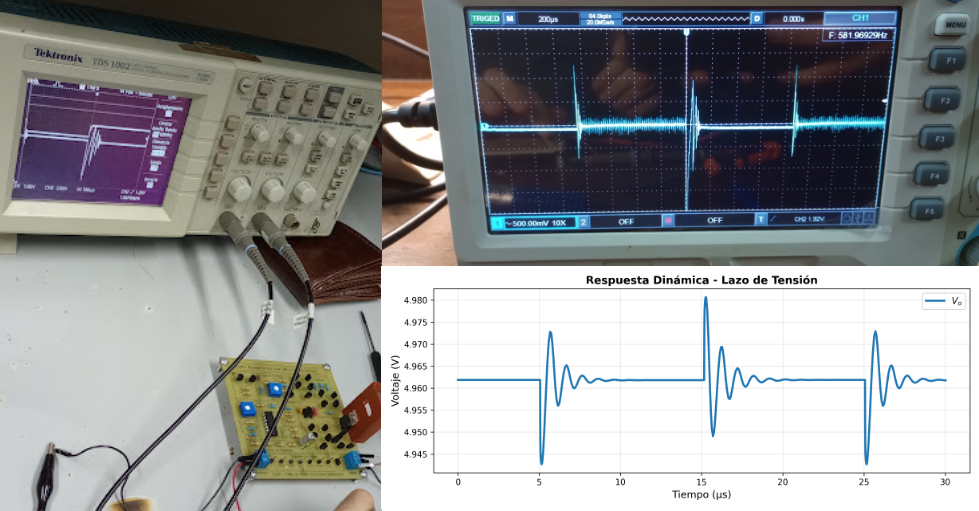
\includegraphics[width=0.95\linewidth]{img/LDO/carga_activa_Medicion}
		\caption{Validación de respuesta dinámica en el laboratorio.}
		\label{fig:cargaactivamedicion}
	\end{figure}
	
	
	\subsubsection{Regulación de línea}
	
	Midiendo de la misma forma que en la figura \ref{fig:medicionregcargabanco} las coordenadas de dos puntos de la curva de tensión de salida en función de la tensión de alimentación es posible calcular la regulación de línea. La estabilización de la tensión de salida resulta algo dependiente de la tensión de la fuente de entrada. Debido a esto, el rechazo del rizado de la fuente de entrada será bajo. Se puede observar la interpolación de los puntos medidos en la figura \ref{fig:regulaciondelinea}.
	
	Se caracteriza la regulación de linea tomando la variación de la salida respecto a la variación de la fuente para dos puntos. En este caso se utilizaron los puntos en donde la tensión de alimentación es de $5,03 \, V$ y  $15,94 \, V$. Obteniendo el valor de $0,035 \frac{V}{V}$ que caracteriza la regulación de linea.
	
	
	% Agregar para comparar con la simulación
	
	\begin{figure}[H]
		\centering
		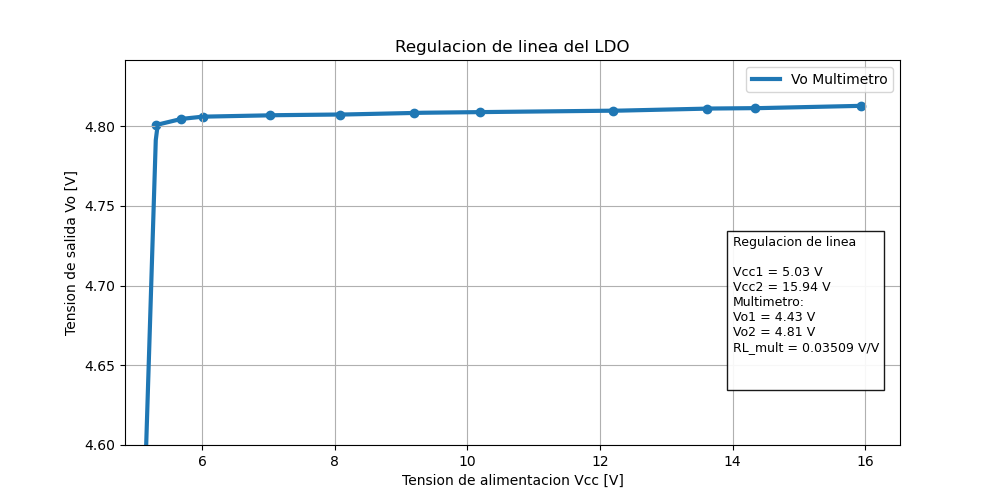
\includegraphics[width=1\linewidth]{../Graficos/regulacion_de_linea}
		\caption{Interpolación de los puntos medidos en regulación de linea.}
		\label{fig:regulaciondelinea}
	\end{figure}
	
	
	\[
	Reg_{\text{mult}} = \frac{V_{O2,\text{mult}} - V_{O1,\text{mult}}}{V_{CC2} - V_{CC1}} = 0,035 \, \frac{V}{V}
	\]
	
	\subsubsection{Limitación de corriente}
	
	El circuito cuenta con una limitación de corriente que se acciona al alcanzar un valor de corriente estimado y comienza el mecanismo de \textit{foldback} en donde la tensión se ajusta dejando de regular.
	
	
	Este mecanismo se observo al variar la carga y midiendo la corriente a través de un amperímetro.
	
	\begin{figure}[H]
		\centering
		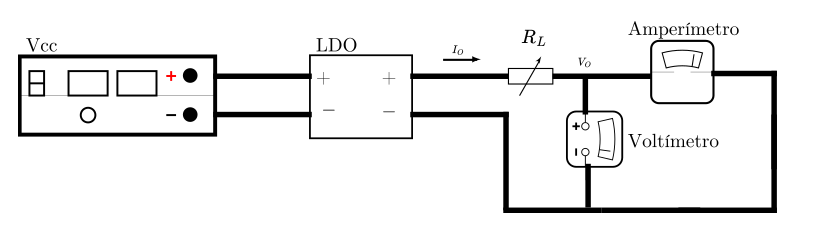
\includegraphics[width=1\linewidth]{img/LDO/Diagramas medicion/corriente}
		\caption{Disposición banco de pruebas para medir corriente y tensión de salida.}
		\label{fig:corriente}
	\end{figure}
	
	
	\begin{figure}[H]
		\centering
		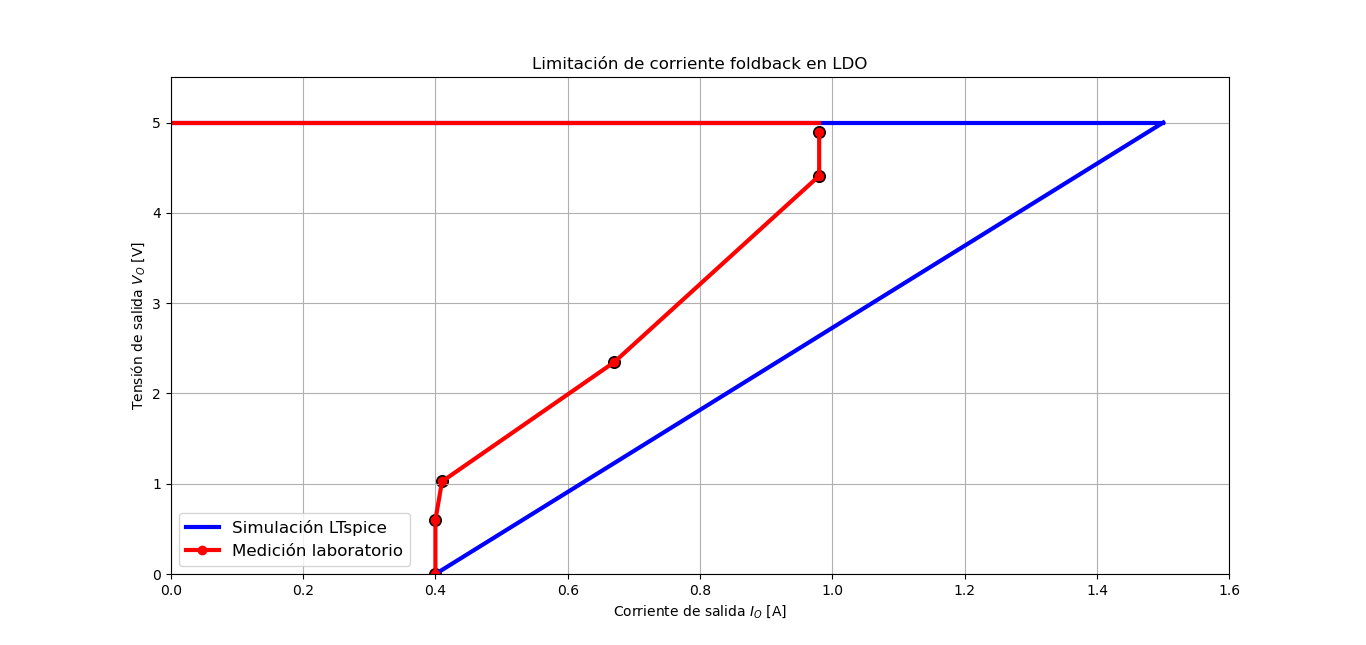
\includegraphics[width=1\linewidth]{../Graficos/regulacion_corriente}
		\caption{Comparación entre lo esperado idealmente en regulación de corriente y lo logrado en el laboratorio al medir el prototipo.}
		\label{fig:regulacioncorriente}
	\end{figure}
	
	
	Se puede observar en la figura \ref{fig:regulacioncorriente} como la medición se desvía respecto a lo esperado, alcanzando un valor máximo de corriente al rededor de 1 A, mientras que se conserva el limite en corto de unos 400 mA previsto en el diseño.
	
	En la tabla \ref{tab:foldback_medicion} se detallan los valores de resistencia contemplados y la corriente de salida alcanzada en los que se baso la interpolación.
	
	\begin{table}[H]
		\centering
		\caption{Mediciones experimentales de foldback en LDO variando la carga}
		\begin{tabular}{|c|c|c|}
			\hline
			\textbf{Resistencia $R_L$ [$\Omega$]} &
			\textbf{Corriente $I_O$ [mA]} &
			\textbf{Tensión $V_O$ [V]} \\
			\hline
			
			0 (corto) & 400 & 0.00 \\
			1.5       & 400 & 0.60 \\
			2.5       & 410 & 1.03 \\
			3.5       & 670 & 2.34 \\
			4.5       & 980 & 4.41 \\
			5.0       & 980 & 4.90 \\
			
			\hline
		\end{tabular}
		\label{tab:foldback_medicion}
	\end{table}
	
	\subsubsection{Eficiencia}
	
	En un regulador lineal de bajo \textit{dropout} (LDO), la eficiencia se define como el cociente entre la potencia entregada a la carga y la potencia absorbida desde la fuente de alimentación, expresada como:
	
	\[
	\eta = \frac{P_O}{P_E} = \frac{V_O I_O}{V_{CC} I_{CC}}
	\]
	
	Debido a que un LDO regula la tensión disipando la diferencia de potencial entre la entrada y la salida sobre el transistor de paso, su eficiencia suele ser menor que la de reguladores conmutados. En particular, la potencia no aprovechada se transforma principalmente en calor. Por este motivo, la eficiencia depende fuertemente de la relación entre la tensión de salida y la tensión de entrada, alcanzando sus mejores valores cuando $V_{CC}$ es apenas superior a $V_O$, es decir, dentro de la zona de regulación cercana al \textit{dropout}. A medida que aumenta la diferencia entre entrada y salida, la disipación interna crece y la eficiencia disminuye considerablemente.
	
	\begin{figure}[H]
		\centering
		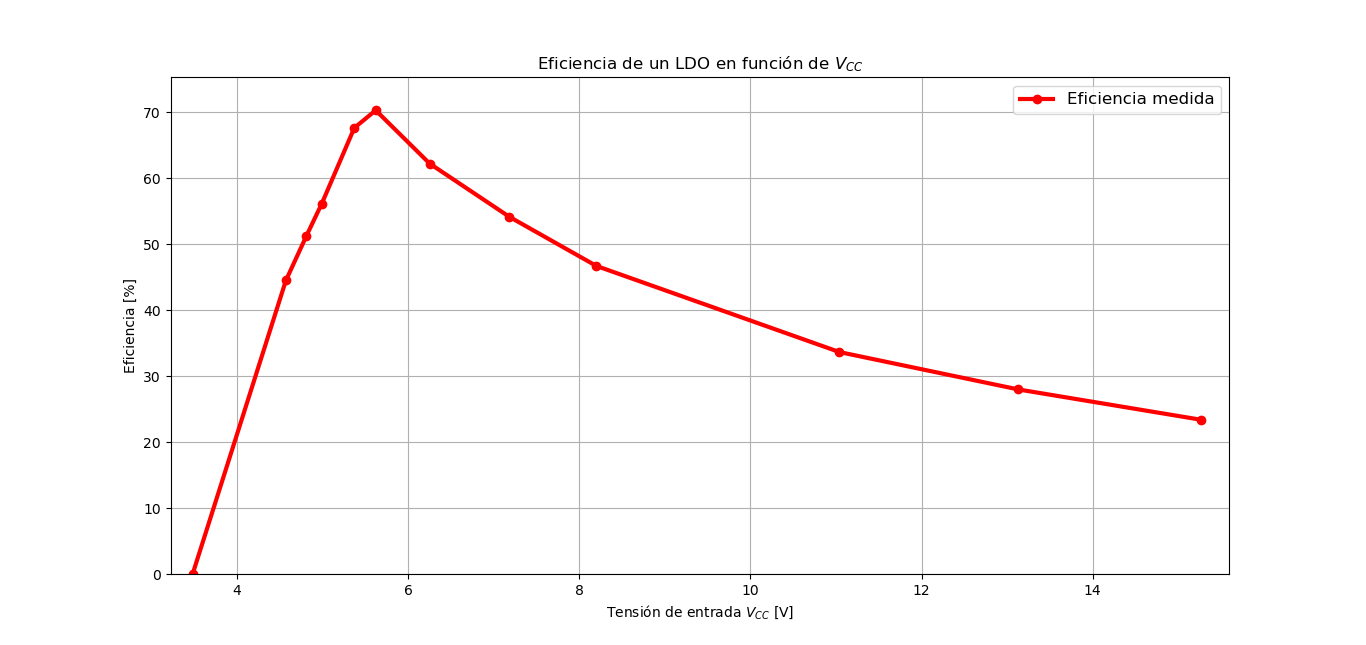
\includegraphics[width=1\linewidth]{../Graficos/eficiencia}
		\caption{}
		\label{fig:eficiencia}
	\end{figure}
	
	\begin{table}[H]
		\centering
		\caption{Mediciones de eficiencia del regulador LDO variando $V_{CC}$}
		\begin{tabular}{|c|c|c|c|c|}
			\hline
			\textbf{$V_{CC}$ [V]} &
			\textbf{$I_{CC}$ [mA]} &
			\textbf{$V_O$ [V]} &
			\textbf{$I_O$ [mA]} &
			\textbf{$P_O/P_E$ [-]} \\
			\hline
			
			3.48  & 20 & 0.0203 & 0.0002 & 0.000058 \\
			4.57  & 34 & 2.63   & 26.3   & 0.417 \\
			4.81  & 41 & 3.18   & 31.8   & 0.506 \\
			4.99  & 47 & 3.63   & 36.3   & 0.561 \\
			5.37  & 59 & 4.63   & 46.3   & 0.642 \\
			5.62  & 63 & 4.99   & 49.9   & 0.704 \\
			6.25  & 64 & 4.99   & 49.9   & 0.620 \\
			7.18  & 64 & 4.99   & 49.9   & 0.544 \\
			8.20  & 65 & 4.99   & 49.9   & 0.469 \\
			11.04 & 67 & 4.99   & 49.9   & 0.336 \\
			13.13 & 68 & 5.00   & 49.99  & 0.280 \\
			15.27 & 70 & 5.00   & 50.0   & 0.232 \\
			\hline
		\end{tabular}
		\label{tab:eficiencia_ldo}
	\end{table}
	\subsection{BUCK}
	\subsubsection{PWM}
	
	
	Ya en el laboratorio se verifica el funcionamiento del PWM, alimentando el circuito con fuentes de laboratorio y utilizando un osciloscopio para observar y medir la señal como se puede ver en la figura \ref{fig:bancopruebaspwm}. Para verificar la modulación del ancho de pulso se coloco una fuente a la terminal de muestreo y se vario la tensión levemente.
	
	\begin{figure}[H]
		\centering
		
\includegraphics[width=0.7\linewidth]{img/buck/banco_pruebas_pwm}
		\caption{Banco de pruebas.}
		\label{fig:bancopruebaspwm}
	\end{figure}
	
	
	Se puede observar la señal triangular y el pulso modulado en la figura \ref{fig:capturasoscpwm}
	
	\begin{figure}[H]
		\centering
		
\includegraphics[width=0.6\linewidth]{img/buck/capturas_osc_pwm}
		\caption{Capturas del osciloscopio midiendo el pulso modulado y la señal triangular del oscilador.}
		\label{fig:capturasoscpwm}
	\end{figure}
	
	Notar que, según el esquemático de la imagen \ref{sec:apendice_PCB}, el comparador con histéresis de la imagen \ref{fig:amp_error} no se encuentra implementado. Esto hace el flanco de conmutación muy ruidoso, debido a la naturaleza también ruidosa de la señal de entrada $v_{sense}$.
	
	\subsubsection{Medición y caracterización del inductor fabricado}
	
	Para corroborar el valor final y el correcto funcionamiento del inductor inicialmente se realizo una medida estimativa del valor de inductancia mediante un circuito que releve un valor aproximado de este y también la no saturación del mismo en condiciones similares a las del circuito regulador. Y como verificación final se realizo una medida con el instrumento de medición de inductancia LCR.
	
	
	\paragraph{Método de medición mediante filtro RL:} 
	
	Se realizo un filtro RL y se comprobó la frecuencia de corte, de esta forma se despejo el valor aproximado de L.
	
	Para determinar la inductancia se emplea un circuito RL serie, excitado
	mediante una señal senoidal de frecuencia variable. Tomando la salida
	sobre el inductor, el circuito se comporta como un filtro pasa-altos cuya
	función de transferencia está dada por
	
	\begin{equation}
		H(s)=\frac{V_L(s)}{V_{in}(s)}=
		\frac{sL}{R+sL}.
	\end{equation}
	
	La frecuencia de corte del filtro se produce cuando la magnitud de la
	impedancia inductiva es igual a la resistencia, es decir,
	
	\begin{equation}
		\omega_cL=R.
	\end{equation}
	
	Como $\omega_c=2\pi f_c$, la inductancia puede obtenerse despejando
	
	\begin{equation}
		L=\frac{R}{2\pi f_c}.
	\end{equation}
	
	De esta manera, conociendo el valor de la resistencia y midiendo la
	frecuencia de corte del circuito, es posible determinar el valor de la
	inductancia. La frecuencia de corte puede identificarse cuando la amplitud de la tensión de salida alcanza el $70.7 \%$ de su valor máximo
	($-3\,\mathrm{dB}$).
	\begin{figure}[H]
		\centering
		
		\begin{minipage}[c]{0.45\textwidth}
			\centering
			\begin{tikzpicture}[transform shape, scale=0.85]
				% Paths, nodes and wires:
				\draw (5, 10.75) to[sinusoidal voltage source, l_={$Señal$}] (5, 13.75);
				\node[ground] at (5, 10.75){};
				\draw (8, 13) to[american resistor, l={$R$}] (8, 15.25);
				\draw (5, 13.75) -| (5, 15.5) -| (8, 15.25);
				\draw (9.75, 11) to[oscope, l_={$Osciloscopio$}] (9.75, 13);
				\draw (8, 13) to[american inductor, l={$L_x$}] (8, 11.25);
				\node[ground] at (8, 10.75){};
				\draw (8, 10.75) -- (8, 11.25);
				\draw (9.75, 11) |- (8, 11);
				\draw (9.75, 13) -- (8, 13);
			\end{tikzpicture}
		\end{minipage}
		\hfill
		\begin{minipage}[c]{0.50\textwidth}
			\centering
			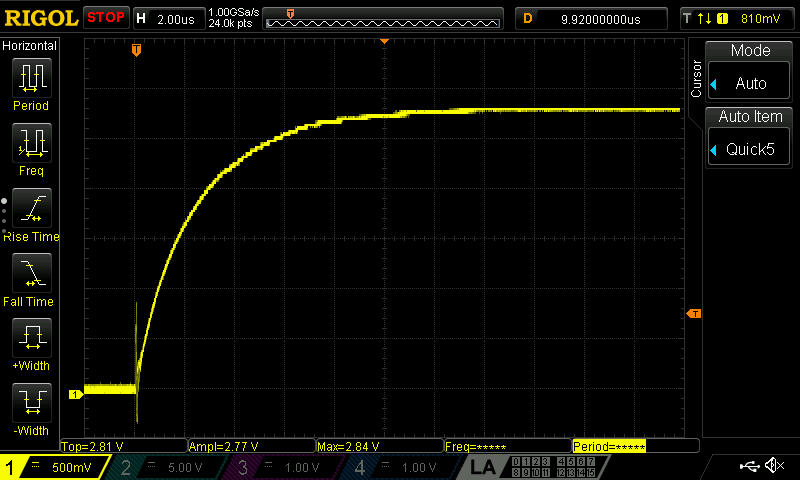
\includegraphics[width=\linewidth]{img/BUCK/inductor_medicion_1}
		\end{minipage}
		
		\caption{Montaje experimental para la medición de la inductancia mediante un circuito RL y captura de la respuesta obtenida en el osciloscopio.}
		\label{fig:inductormedicion1}
	\end{figure}
	
	
	\paragraph{Método contemplando linealidad y saturación: } 
	
	
	La Figura \ref{fig:medicion_L_sat} presenta el circuito utilizado para verificar la linealidad del inductor mediante un ensayo de corriente pulsada (\textit{Pulse Test}). El MOSFET conmuta el inductor mediante una señal PWM, mientras que el diodo proporciona un camino de circulación para la corriente durante el apagado del transistor. La corriente del inductor se obtiene midiendo la tensión sobre la resistencia de sensado $R_{sense}$. Incrementando gradualmente la tensión de alimentación o el tiempo de conducción del MOSFET, la corriente alcanza valores cada vez mayores. Mientras el núcleo opere en la región lineal, la corriente presenta una rampa de pendiente constante; la aparición de una curvatura creciente indica el inicio de la saturación del núcleo debido a la disminución de la inductancia efectiva. El valor de L se obtiene calculando la pendiente de dicha curva.
	
	Durante el intervalo de conducción del MOSFET, la tensión aplicada al
	inductor puede aproximarse por
	
	\begin{equation}
		v_L \approx V_{CC}.
	\end{equation}
	
	A partir de la ecuación característica del inductor,
	
	\begin{equation}
		v_L=L\frac{di_L}{dt},
	\end{equation}
	
	despejando la inductancia se obtiene
	
	\begin{equation}
		L=\frac{v_L}{\dfrac{di_L}{dt}}
		\approx
		\frac{V_{CC}}{\dfrac{di_L}{dt}}.
	\end{equation}
	
	\begin{figure}[H]
		
		\begin{minipage}[t]{0.42\textwidth}
			\centering
			\begin{tikzpicture}[transform shape, scale=0.95]
				% Paths, nodes and wires:
				\draw (5.75, 12) to[empty diode, l={$D$}] (5.75, 14.5);
				\draw (8.25, 14.75) to[american inductor, l={$L$}] (8.25, 12);
				\draw (8.25, 11.375) -| (8.25, 11.5);
				\node[nmos, xscale=-1, yscale=-1](N1) at (8.25, 10.605){} node[anchor=east] at (N1.text){$Q$};
				\draw (8.25, 9.835) to[american resistor, /tikz/circuitikz/bipoles/length=1.16cm, l={$R_{sense}$}] (8.25, 7.25);
				\node[ground] at (8.25, 7.25){};
				\node[ground] at (3.25, 13.75){};
				\draw (3.25, 15.75) -- (7, 15.75) -| (7, 15.25);
				\draw (3.25, 15.75) to[american voltage source, l={$V_{cc}$}] (3.25, 13.75);
				\draw (10.5, 9.25) to[square voltage source, l={$V_s$}] (10.5, 10.25);
				\node[ground] at (10.5, 9.25){};
				\draw (9.23, 10.605) -| (10.5, 10.25);
				\draw (8.25, 14.75) -| (8.25, 15.25) -- (7, 15.25);
				\draw (5.75, 14.5) -| (5.75, 15.25) -- (7, 15.25);
				\draw (5.75, 12) -- (8.25, 12);
				\draw (8.25, 11.5) -| (8.25, 12);
			\end{tikzpicture}
		\end{minipage}
		\hfill
		\begin{minipage}[t]{0.5\textwidth}
			\vspace*{-6cm}
			Se observa la tensión sobre la resistencia de sensado
			$R_{sense}$, proporcional a la corriente del inductor.
			Mientras el núcleo permanezca en la región lineal, la corriente
			debe aumentar formando una rampa de pendiente constante.
			
			
			\begin{enumerate}
				\item Se fija una tensión continua $V_{cc}$.
				\item Se excita el MOSFET con un PWM de \textit{Duty} ajustable mediante generador digital.
				\item Medir la tensión sobre $R_{sense}$.
				\item Incrementar gradualmente $V_{cc}$ o el ciclo de trabajo \textit{Duty}.
			\end{enumerate}
			
			Si la rampa permanece lineal, el núcleo opera fuera de saturación. La aparición de una curvatura creciente indica el inicio de la saturación del núcleo.
			
		\end{minipage}
		
		\caption{Circuito para la medición de la saturación del inductor mediante corriente pulsada.}
		\label{fig:medicion_L_sat}
	\end{figure}
	
	
	\paragraph{Medición mediante LCR:}
	
	Finalmente, la inductancia como ultima instancia se verificó mediante un medidor LCR ( Fig.\ref{fig:medicionlcr}), el cual determina el valor del componente aplicando una señal senoidal de pequeña amplitud y midiendo su impedancia compleja. A partir de la reactancia inductiva y la frecuencia de ensayo, el instrumento calcula automáticamente la inductancia. Este método proporciona una medición de mayor precisión y sirve para validar el valor obtenido mediante los métodos anteriores.
	
	
	
	La siguiente lista detalla las consideraciones para establecer la medición del LCR como la mas precisa.
	\begin{itemize}
		\item Frecuencia de prueba conocida y estable. El instrumento genera una señal senoidal de amplitud y frecuencia muy precisas (100 Hz, 120 Hz, 1 kHz, 10 kHz o 100 kHz).
		\item Medición simultánea de tensión y corriente. Mide con gran precisión la amplitud y el desfase entre ambas magnitudes.
		\item Procesamiento digital. A partir de estas mediciones calcula la impedancia compleja del componente y obtiene directamente la inductancia, la resistencia serie equivalente (ESR) y el factor de calidad (Q).
		
		\item Calibración interna. Los medidores LCR compensan las resistencias y capacitancias de los cables mediante procedimientos de calibración (\textit{open} y \textit{short}), reduciendo significativamente el error.
		
	\end{itemize}
	
	
	\begin{figure}[H]
		\centering
		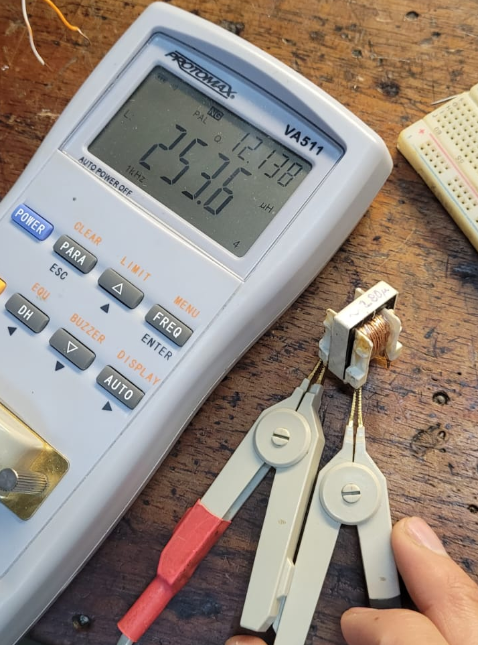
\includegraphics[width=0.3\linewidth]{img/BUCK/medicion_LCR}
		\caption{Medición de inductancia mediante instrumento LCR.}
		\label{fig:medicionlcr}
	\end{figure}
	
	\subsubsection{Regulación de linea}
	
	La regulación de línea caracteriza la capacidad del convertidor para mantener constante la tensión de salida frente a variaciones en la tensión de entrada, manteniendo constante la carga en este caso de $1 \, k\Omega$, cabe resaltar que se encuentra en paralelo con la resistencia de sangrado interna de $100\, \Omega$. Rápidamente se detecto un error en el rendimiento de la fuente, ya que la regulación comienza a partir de una entrada de 13 V, mayor a lo esperado en el diseño el cual regulaba para valores mas bajos llegando a cumplir el requerimiento del rango de entrada desde 12 V hasta 30 V. Por otra parte las mediciones se ven limitadas hasta un valor cercano a 24 V debido a limitación del instrumental utilizado en el laboratorio.
	
	
	
	Debido a que las variaciones de la tensión de salida son del orden de unos pocos milivoltios, en lugar de medir directamente la tensión de salida se utilizó una fuente de laboratorio auxiliar ajustada a $9.5\,\mathrm{V}$ como referencia. Para cada valor de tensión de entrada se midió la diferencia de potencial entre la salida del convertidor \textit{buck} y la fuente de laboratorio, obteniendo el error $\Delta V_o$. Posteriormente, la tensión de salida se reconstruyó como
	
	\[
	V_o = 9.5\,\mathrm{V} + \Delta V_o,
	\]
	
	lo que permitió representar gráficamente la regulación de línea con mayor resolución.
	
	La regulación de línea se estimó a partir de la pendiente promedio de la característica de transferencia,
	
	\[
	\mathrm{Reg}_{\mathrm{L}}=
	\frac{\Delta V_o}{\Delta V_{in}},
	\]
	
	obteniéndose
	
	\[
	\mathrm{Reg}_{\mathrm{L}}
	=
	\frac{66.1\,\mathrm{mV}}{10.78\,\mathrm{V}}
	=
	6.13\,\mathrm{mV/V}.
	\]
	
	Este resultado indica que, en promedio, la tensión de salida varía aproximadamente $6.13\,\mathrm{mV}$ por cada voltio de variación de la tensión de entrada, evidenciando un aceptable comportamiento del convertidor frente a perturbaciones en la alimentación.
	
	
	\begin{figure}[H]
		\centering
		
		\begin{minipage}[t]{0.58\textwidth}
			\centering
			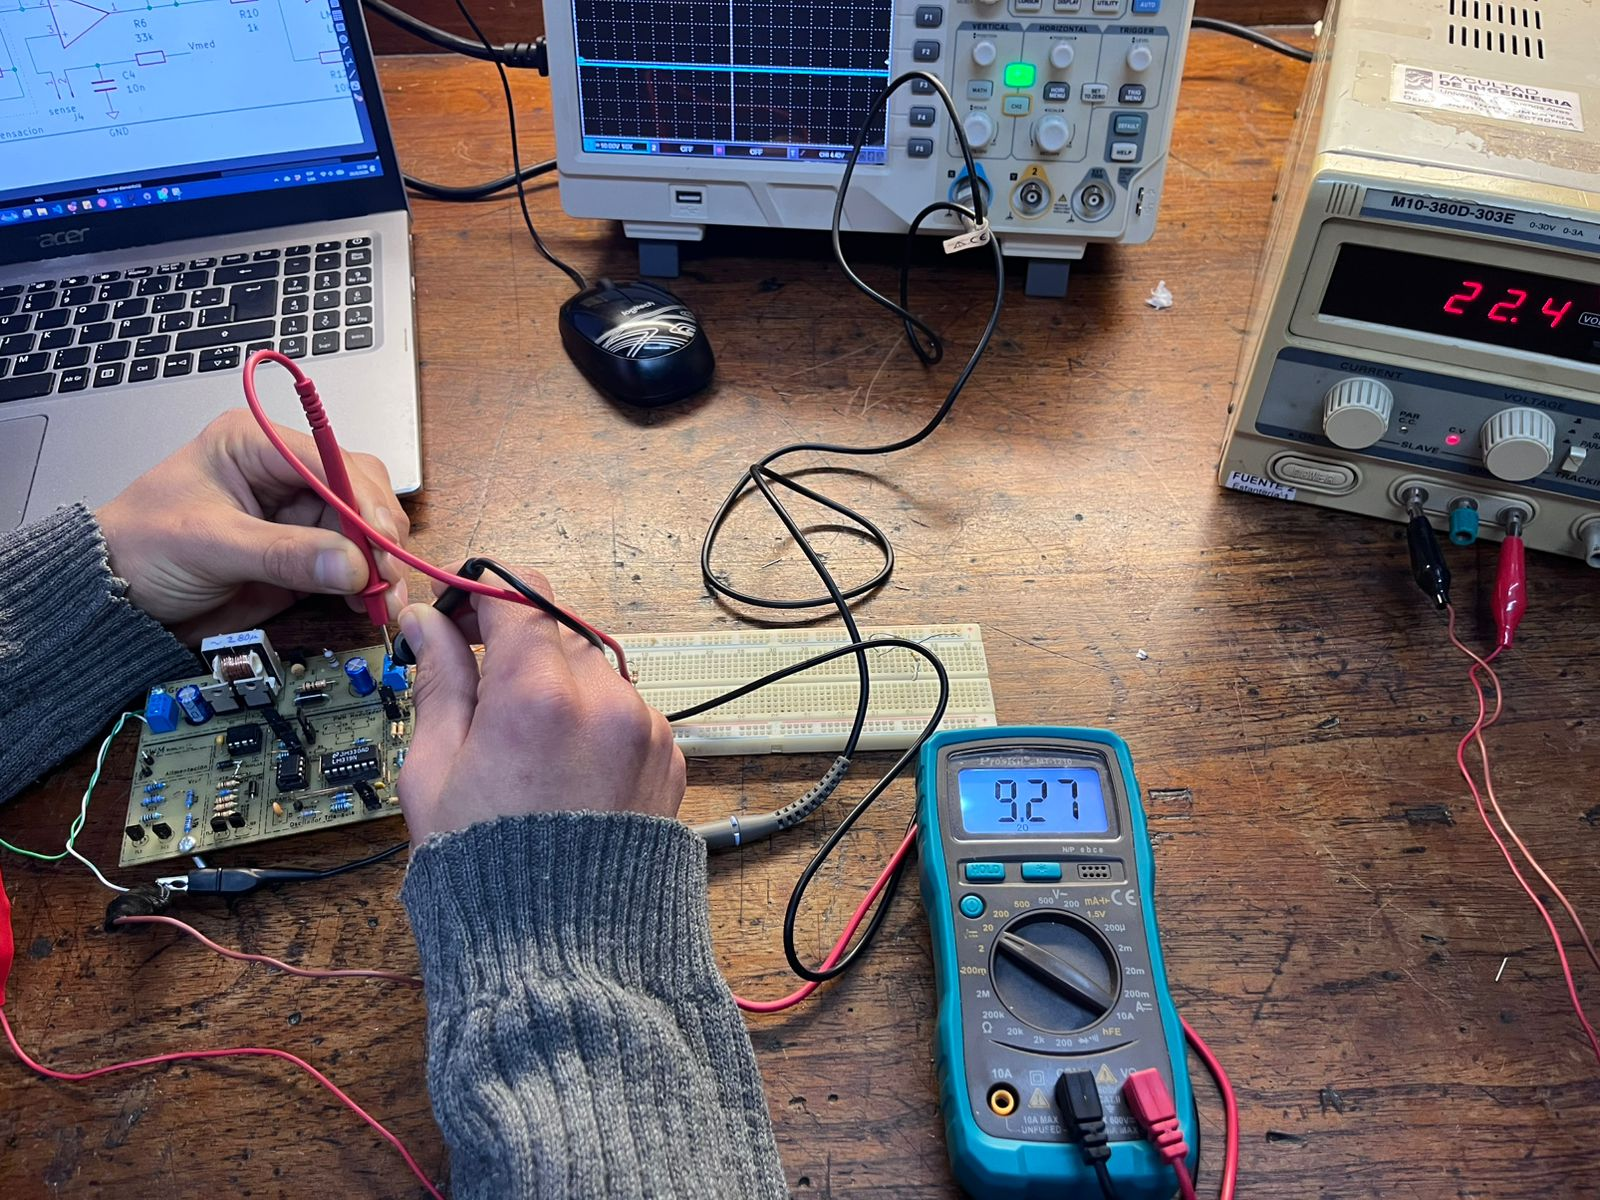
\includegraphics[width=\linewidth]{img/BUCK/regulacion_tension}
			\caption{Medición inicial de la regulación para una tensión dentro de entrada de 22 V.}
			\label{fig:regulaciontension}
		\end{minipage}
		\hfill
		\begin{minipage}[t]{0.38\textwidth}
			\centering
			\vspace{-8cm}
			\captionof{table}{Mediciones de regulación de línea.}
			\label{tab:regulacion_linea}
			\begin{tabular}{cc}
				\toprule
				$V_{in}$ [V] & $\Delta V_o$ [mV] \\
				\midrule
				13.32 & -78.0 \\
				14.27 & -37.7 \\
				15.32 & -32.5 \\
				16.37 & -30.4 \\
				17.42 & -22.3 \\
				18.34 & -17.5 \\
				19.59 & -17.7 \\
				20.10 & -17.8 \\
				21.30 & -15.2 \\
				22.20 & -12.0 \\
				23.30 & -12.2 \\
				24.10 & -11.9 \\
				\bottomrule
			\end{tabular}
		\end{minipage}
		
	\end{figure}
	
	
	\begin{figure}[H]
		\centering
		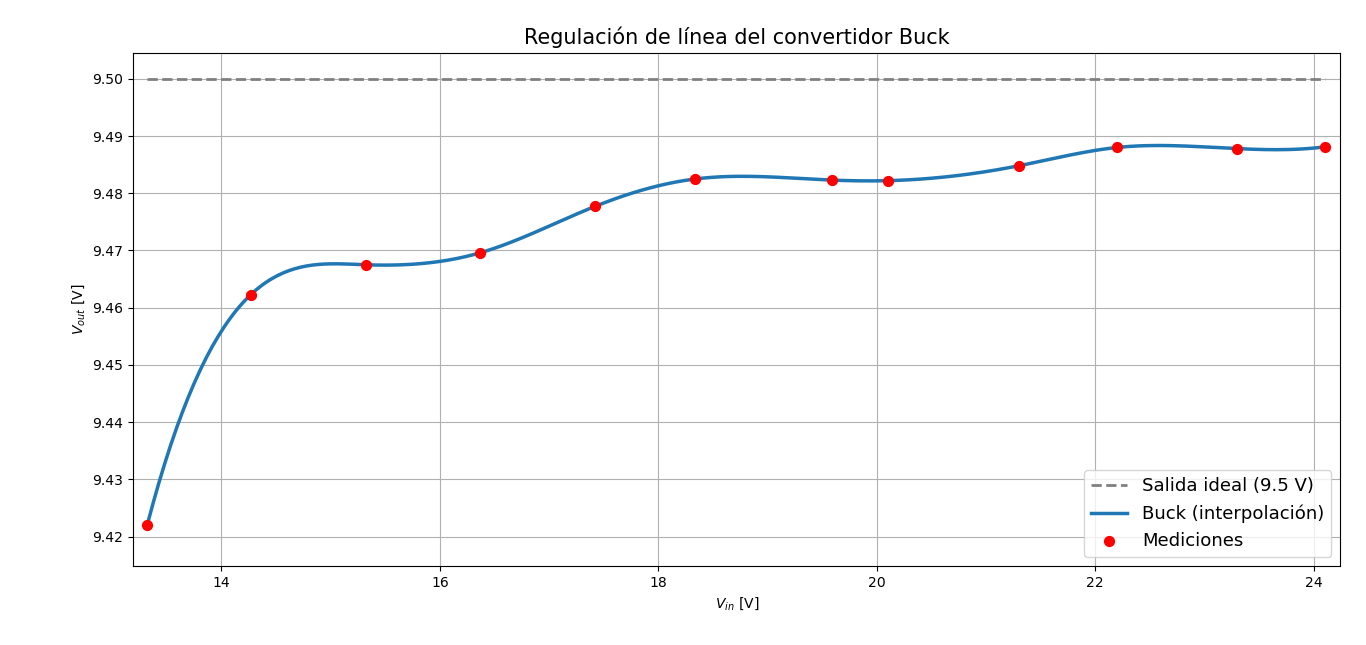
\includegraphics[width=1\linewidth]{img/BUCK/mediciones interpolaciones/regulacion_linea}
		\caption{Interpolación de los puntos medidos.}
		\label{fig:regulacionlinea}
	\end{figure}
	
	En función de los resultados obtenidos, apreciables en la tabla \ref{tab:regulacion_linea}, el convertidor mantiene la tensión de salida dentro del rango especificado de 9.3 V a 9.7 V para todas las condiciones de entrada ensayadas, comprendidas entre \(13.32\,\mathrm{V}\) y \(24.10\,\mathrm{V}\). Sin embargo, se verificó experimentalmente que el convertidor no comienza a regular a partir de \(12\,\mathrm{V}\), como se establecía en las especificaciones de diseño, sino aproximadamente desde \(13\,\mathrm{V}\). Asimismo, debido a la limitación de la fuente de alimentación disponible en el laboratorio, no fue posible extender las mediciones hasta \(30\,\mathrm{V}\), por lo que el cumplimiento de la regulación de línea para el intervalo comprendido entre \(24.10\,\mathrm{V}\) y \(30\,\mathrm{V}\) no pudo ser corroborado experimentalmente.
	
	
	\subsubsection{Regulación de carga}
	
	La \textbf{regulación de carga} es un parámetro que cuantifica la capacidad de una fuente de alimentación para mantener constante su tensión de salida frente a variaciones en la corriente demandada por la carga. La tensión de salida debe experimentar una variación mínima de $\Delta V_0 = 400 \, mV$ al pasar desde condiciones de carga ligera $100 \, mA$ hasta carga nominal de $1.5 \,A$ según las condiciones establecidas. La carga ensayada consto de un reóstato, es decir una resistencia variable diseñada específicamente para controlar y regular la intensidad de la corriente eléctrica en un circuito, el banco de ensayo se observa en la figura \ref{fig:bancomedicionregcarga}.
	
	\begin{figure}[H]
		\centering
		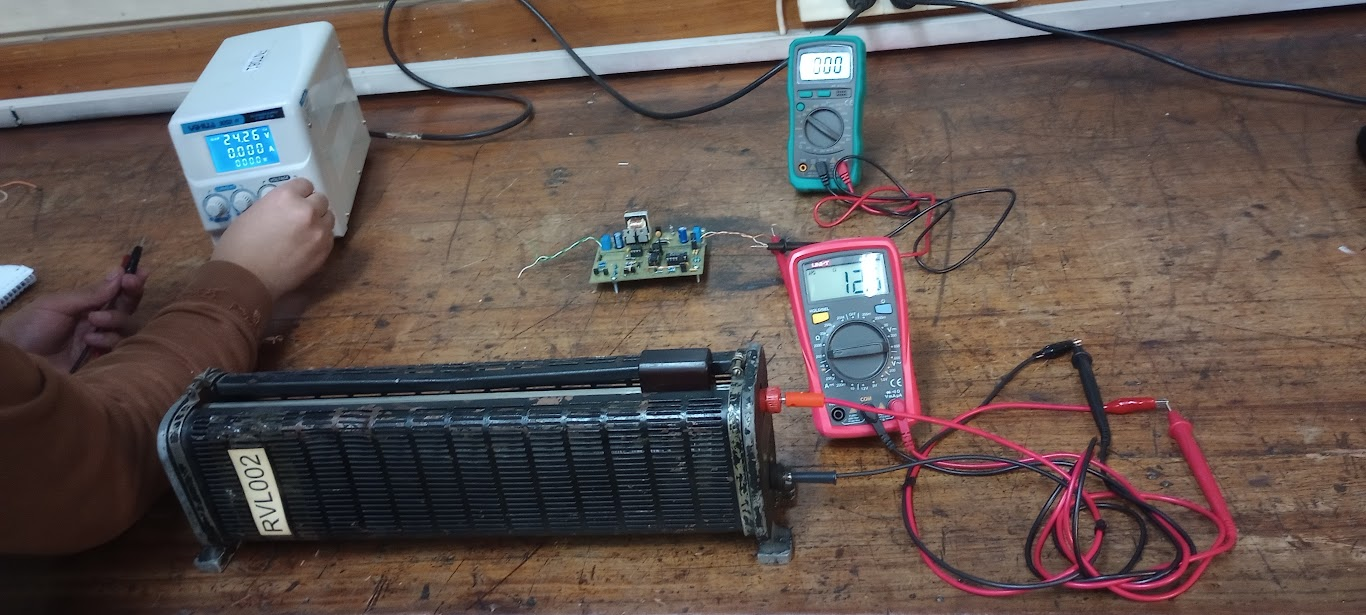
\includegraphics[width=0.7\linewidth]{img/BUCK/banco_medicion_reg_carga}
		\caption{Banco de medición de regulación de carga.}
		\label{fig:bancomedicionregcarga}
	\end{figure}
	
	
	Durante el ensayo de regulación de carga se observó que el convertidor mantuvo una tensión de salida prácticamente constante para corrientes inferiores a aproximadamente $700\,\mathrm{mA}$. Sin embargo, al incrementar la carga por encima de dicho valor, la fuente dejó de regular adecuadamente, produciéndose una caída abrupta de la tensión de salida, acompañada de un incremento significativo de la corriente consumida, dando indicios de que el convertidor entraba en una condición cercana a un cortocircuito.
	
	Con el objetivo de analizar este comportamiento, se monitoreó mediante osciloscopio la señal $V_S$ correspondiente a la salida del \textit{gate driver}. Se observó que, al aumentar la carga, el tiempo de conducción del transistor se incrementaba progresivamente hasta aproximarse al período completo de conmutación ($T_s$), es decir, el ciclo de trabajo tendía a valores cercanos al $100 \%$. Este comportamiento indica que el lazo de control intentaba compensar la caída de la tensión de salida aumentando continuamente el ciclo de trabajo, sin lograr recuperar la regulación.
	
	Adicionalmente, se observó que la señal triangular generada por el oscilador presentaba un nivel considerable de ruido únicamente cuando el convertidor operaba con estas cargas elevadas. Este fenómeno podría afectar el funcionamiento del comparador PWM, provocando fluctuaciones del ciclo de trabajo e incluso situaciones de saturación del modulador.
	
	Si bien no fue posible determinar experimentalmente la causa exacta de esta pérdida de regulación, existen diversas hipótesis que podrían explicar el comportamiento observado:
	
	\begin{itemize}
		\item Saturación del inductor, provocando una disminución abrupta de la inductancia efectiva y un incremento excesivo de la corriente.
		
		\item Insuficiente compensación del lazo de control, originando una respuesta inestable para corrientes elevadas.
		
		\item Acoplamiento de ruido de conmutación hacia el circuito de control, especialmente sobre la rampa triangular o la red de realimentación.
		
		\item Disposición física (layout) inadecuada, generando inductancias parásitas y rebotes de masa (\textit{ground bounce}) que afectan las señales analógicas del controlador.
		
		
	\end{itemize}
	
	Para identificar el origen del problema se propone realizar los siguientes ensayos:
	
	\begin{itemize}
		\item Medir la corriente del inductor para verificar la posible aparición de saturación.
		\item Comparar la rampa triangular en vacío y bajo carga utilizando una punta diferencial o minimizando el lazo de masa del osciloscopio.
		\item Medir simultáneamente la tensión de alimentación del controlador y del \textit{gate driver} para descartar caídas de alimentación.
		\item Verificar el funcionamiento del lazo abierto, fijando manualmente el ciclo de trabajo, para comprobar si la etapa de potencia es capaz de entregar la corriente requerida.
		\item Revisar la compensación del amplificador de error mediante simulación y análisis de estabilidad.
		\item Mejorar el desacoplo de la alimentación del circuito de control e implementar una separación más rigurosa entre las masas de potencia y de señal.
	\end{itemize}
	
	
	Se detalla a continuación un esquemático (figura \ref{fig:esquematico_med_reg_carga}) de la medición una vez se de con la solución, de forma de obtener mayor precisión en los datos, tomando mediciones de un $\Delta V_o$ y la corriente en carga.
	
	\begin{figure}[H]
		\centering
		\begin{tikzpicture}[transform shape]
			% Paths, nodes and wires:
			\node[ground] at (7.25, 13){};
			\draw (7.25, 16) to[american voltage source, l={$V_{CC}$}] (7.25, 13);
			\draw (14.5, 16.25) to[voltmeter, v^<=$\Delta V_o$, voltage/bump b=3] (17.75, 16.25);
			\draw (13, 16.25) to[variable american resistor, l_={$\text{Reóstato}$}] (13, 12.75);
			\node[ground] at (13, 12.25){};
			\draw (14.5, 16.25) |- (13, 16.25);
			\draw (9.5, 16.25) to[sdcdc, /tikz/circuitikz/bipoles/length=2.34cm, l={$buck$}] (13, 16.25);
			\node[ground] at (18, 13.25){};
			\draw (18, 16.25) to[american voltage source, l={$9,5 V$}] (18, 13.25);
			\draw (17.75, 16.25) -- (18, 16.25);
			\draw (9.5, 16.25) |- (7.25, 16.25) -| (7.25, 16);
			\draw (13, 12.25) to[ammeter] (13, 13.25);
		\end{tikzpicture}
		\caption{Esquemático del banco de ensayo utilizado para la medición de la regulación de carga del convertidor Buck.}
		\label{fig:esquematico_med_reg_carga}
	\end{figure}
	
	
	La regulación de carga se calcula mediante la siguiente expresión:
	
	\begin{equation}
		\text{Regulación de carga} =
		\frac{V_{\text{carga ligera}}-V_{\text{carga nominal}}}
		{V_{\text{carga nominal}}}
		\times 100 \% \label{eq:reg_carga}
	\end{equation}
	
	donde $V_{\text{carga ligera}}$ corresponde a la tensión de salida medida para una corriente de carga reducida (en este caso $100\,\mathrm{mA}$) y $V_{\text{carga nominal}}$ es la tensión de salida para la corriente máxima especificada ($1.5\,\mathrm{A}$).
	
	Se espera que la tensión permanezca prácticamente constante al variar la carga entre $100\,\mathrm{mA}$ y $1.5\,\mathrm{A}$. En condiciones normales de funcionamiento, una regulación de carga inferior al $1 \% $  se considera un resultado satisfactorio, correspondiendo a una diferencia de tensión inferior a aproximadamente $95\,\mathrm{mV}$ entre ambos extremos del rango de carga.
	
	\subsubsection{Eficiencia}
	
	Para el análisis de eficiencia del circuito, se puede retomar el mismo banco de prueba que para la regulación de carga (Fig.\ref{fig:esquematico_med_reg_carga}) dado que la fuente de laboratorio cuenta con amperímetro integrado y podremos conocer $I_{cc}$, se diferenciara de la anterior medición ya que se tomaran rango de valores de interés y también se variara la tensión de entrada, ya que en las especificaciones debemos garantizar una eficiencia de entre $85 \%$ hasta $97 \%$ para los rangos $V_{cc} \in [12,5 \, V ; 30 \, V]$ y $ I_o \in [750 \, mA ; 1.5 \,A]$.
	
	
	La eficiencia se define como la relación entre la potencia entregada a la carga y la potencia absorbida desde la fuente de alimentación. Este parámetro permite cuantificar el aprovechamiento energético del convertidor, considerando las pérdidas presentes en los dispositivos semiconductores, el inductor, el circuito de control y los elementos pasivos.
	
	La eficiencia puede expresarse mediante
	
	\begin{equation}
		\eta=
		\frac{P_{\mathrm{salida}}}
		{P_{\mathrm{entrada}}}
		\times100 \%
	\end{equation}
	
	donde
	
	\begin{equation}
		P_{\mathrm{entrada}}=V_{CC}\,I_{CC}
	\end{equation}
	
	y
	
	\begin{equation}
		P_{\mathrm{salida}}=V_{o}\,I_{o}.
	\end{equation}
	
	Por lo tanto, la eficiencia puede calcularse experimentalmente mediante
	
	\begin{equation}
		\eta=
		\frac{V_o I_o}
		{V_{CC} I_{CC}}
		\times100 \%
	\end{equation}
	
	Para verificar el cumplimiento de las especificaciones del diseño, se realizarían mediciones de la tensión y corriente de entrada, junto con la tensión y corriente de salida, variando la tensión de alimentación en el intervalo
	
	En cada punto de operación se calcularía la eficiencia mediante la ecuación anterior y posteriormente se gráfica su evolución en función de la tensión de entrada para distintos valores de corriente de carga. De acuerdo con las especificaciones del proyecto, el convertidor debe presentar una eficiencia comprendida dentro de todo el rango de operación especificado.
	
	Idealmente, la eficiencia debería mantenerse elevada en todo el rango de tensiones de entrada, presentando únicamente pequeñas variaciones debido a las pérdidas por conducción del MOSFET y del diodo, las pérdidas de conmutación, las pérdidas magnéticas del inductor y el consumo propio del circuito de control. Como consecuencia, es esperable que la eficiencia disminuya levemente para tensiones de entrada elevadas, debido al incremento de las pérdidas de conmutación, y para cargas reducidas, donde el consumo del circuito de control representa una fracción mayor de la potencia total suministrada.
	
	En cuanto a la curva de eficiencia en función de la tensión de entrada, lo esperable es que la eficiencia se mantenga alta en la mayor parte del rango y disminuya suavemente al aumentar la tensión de entrada. Este comportamiento se explica principalmente por el incremento de las pérdidas de conmutación, por el mayor tiempo de conducción del diodo cuando el ciclo de trabajo disminuye para el \textit{buck} asíncrono y esta característica para el \textit{buck} sincrónico se esperaría que ocurra de forma menos pronunciada. 
	
	\subsubsection{Resultados Parciales}
	Tras la estabilización del circuito (sección \ref{sec:ruido}), se realizan mediciones con diferentes valores de carga, para dar una forma aproximada a la curva de regulación de carga y eficiencia. Dado que no se cuenta con una fuente de alimentación externa, se utiliza un multímetro como muestra la figura \ref{fig:esquematico_med_reg_carga}, pero sin la fuente externa de \SI{9.5}{V}, a costa de perder precisión.
	
	\begin{figure}[H]
		\centering
		\label{tab:regulacion_carga}
		\begin{tabular}{cccccc}
			\toprule
			$V_{in}$ [V] & $ V_o$ [mV] & $I_i$ & $I_o$ & $R_L$ & $\eta$ \\
			\midrule
			\SI{15.19}{V} & \SI{9.53}{V} & \SI{951}{mA} & \SI{1.35}{A} & \SI{6.3}{\ohm} & 89\% \\
			\SI{15.19}{V} & \SI{9.54}{V} & \SI{717}{mA} & \SI{1.02}{A} & \SI{8.8}{\ohm} & 77\% \\
			\SI{15.25}{V} & \SI{9.54}{V} & \SI{608}{mA} & \SI{850}{mA} & \SI{10}{\ohm} & 91\% \\
			\SI{15.25}{V} & \SI{9.54}{V} & \SI{503}{mA} & \SI{700}{mA} & \SI{12}{\ohm} & 87\% \\
			\SI{15.25}{V} & \SI{9.54}{V} & \SI{432}{mA} & \SI{590}{mA} & \SI{15}{\ohm} & 85\% \\
			\SI{15.25}{V} & \SI{9.55}{V} & \SI{185}{mA} & \SI{200}{mA} & \SI{47}{\ohm} & 68\% \\
			\SI{15.25}{V} & \SI{9.55}{V} & \SI{111}{mA} & \SI{95}{mA} & \SI{100}{\ohm} & 53\% \\
			\bottomrule
		\end{tabular}
		\captionof{table}{Mediciones de regulación de carga.}
	\end{figure}
	
	Notar que para el rango de corrientes $\SI{590}{mA} < Io < \SI{1.5}{A}$, la eficiencia se encuentra en el rango esperado, alcanzando valores pico de 91\%, excepto para valores cercanos a \SI{9}{\ohm}.
	
	En cuanto a la regulación de carga, la limitación de medición impide obtener un resultado preciso, pero se puede conjeturar que tendrá un valor de, como máximo, y utilizando la ecuación \ref{eq:reg_carga}:
	
	\begin{equation}
		\frac{\SI{9.56}{V} - \SI{9.53}{V}}{\SI{9.53}{V}} \times 100\% = 0.31\%.
	\end{equation}
	
	Lo cual es una cota superior muy buena.
	
	
	\subsubsection{Red \textit{Snubber}}
	
	\begin{figure}[H]
		\centering
		
		\begin{minipage}{0.48\linewidth}
			\centering
			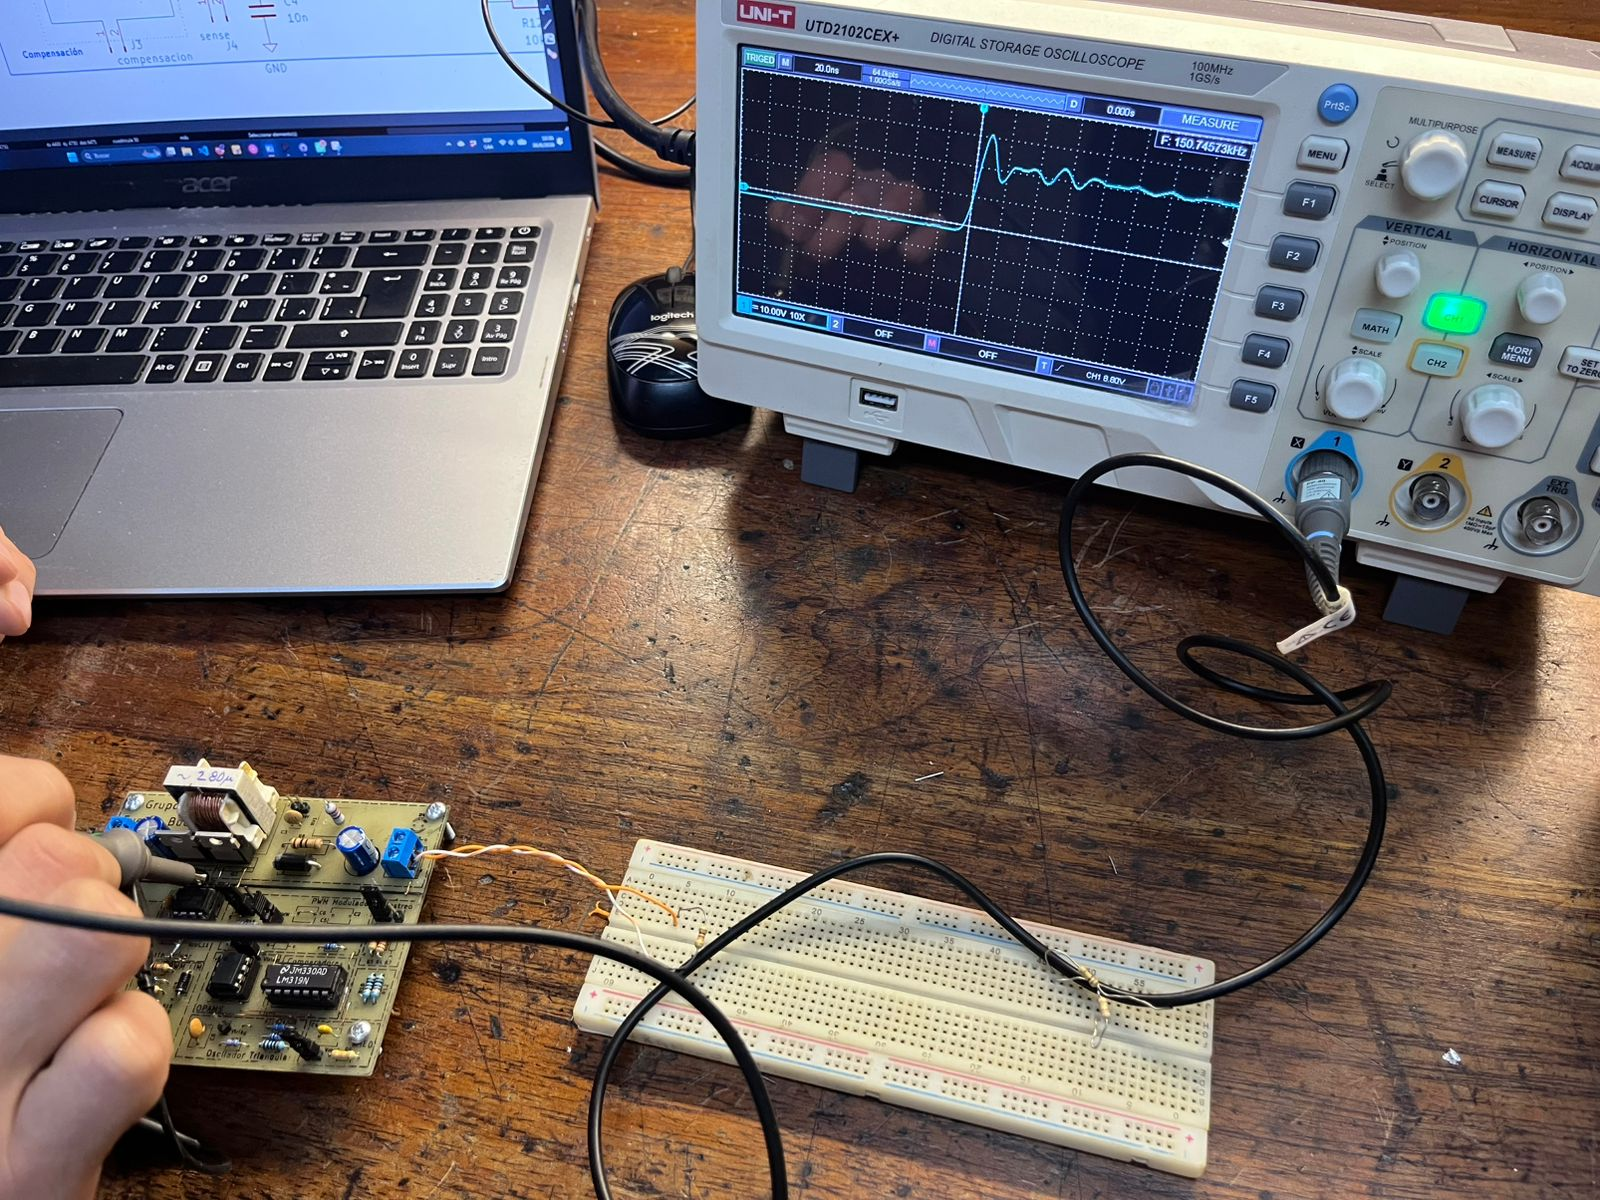
\includegraphics[width=\linewidth]{img/BUCK/medicion_sin_snubber}
			\caption{Medición con red \textit{Snubber}.}
			\label{fig:medicionsinsnubber}
		\end{minipage}
		\hfill
		\begin{minipage}{0.48\linewidth}
			\centering
			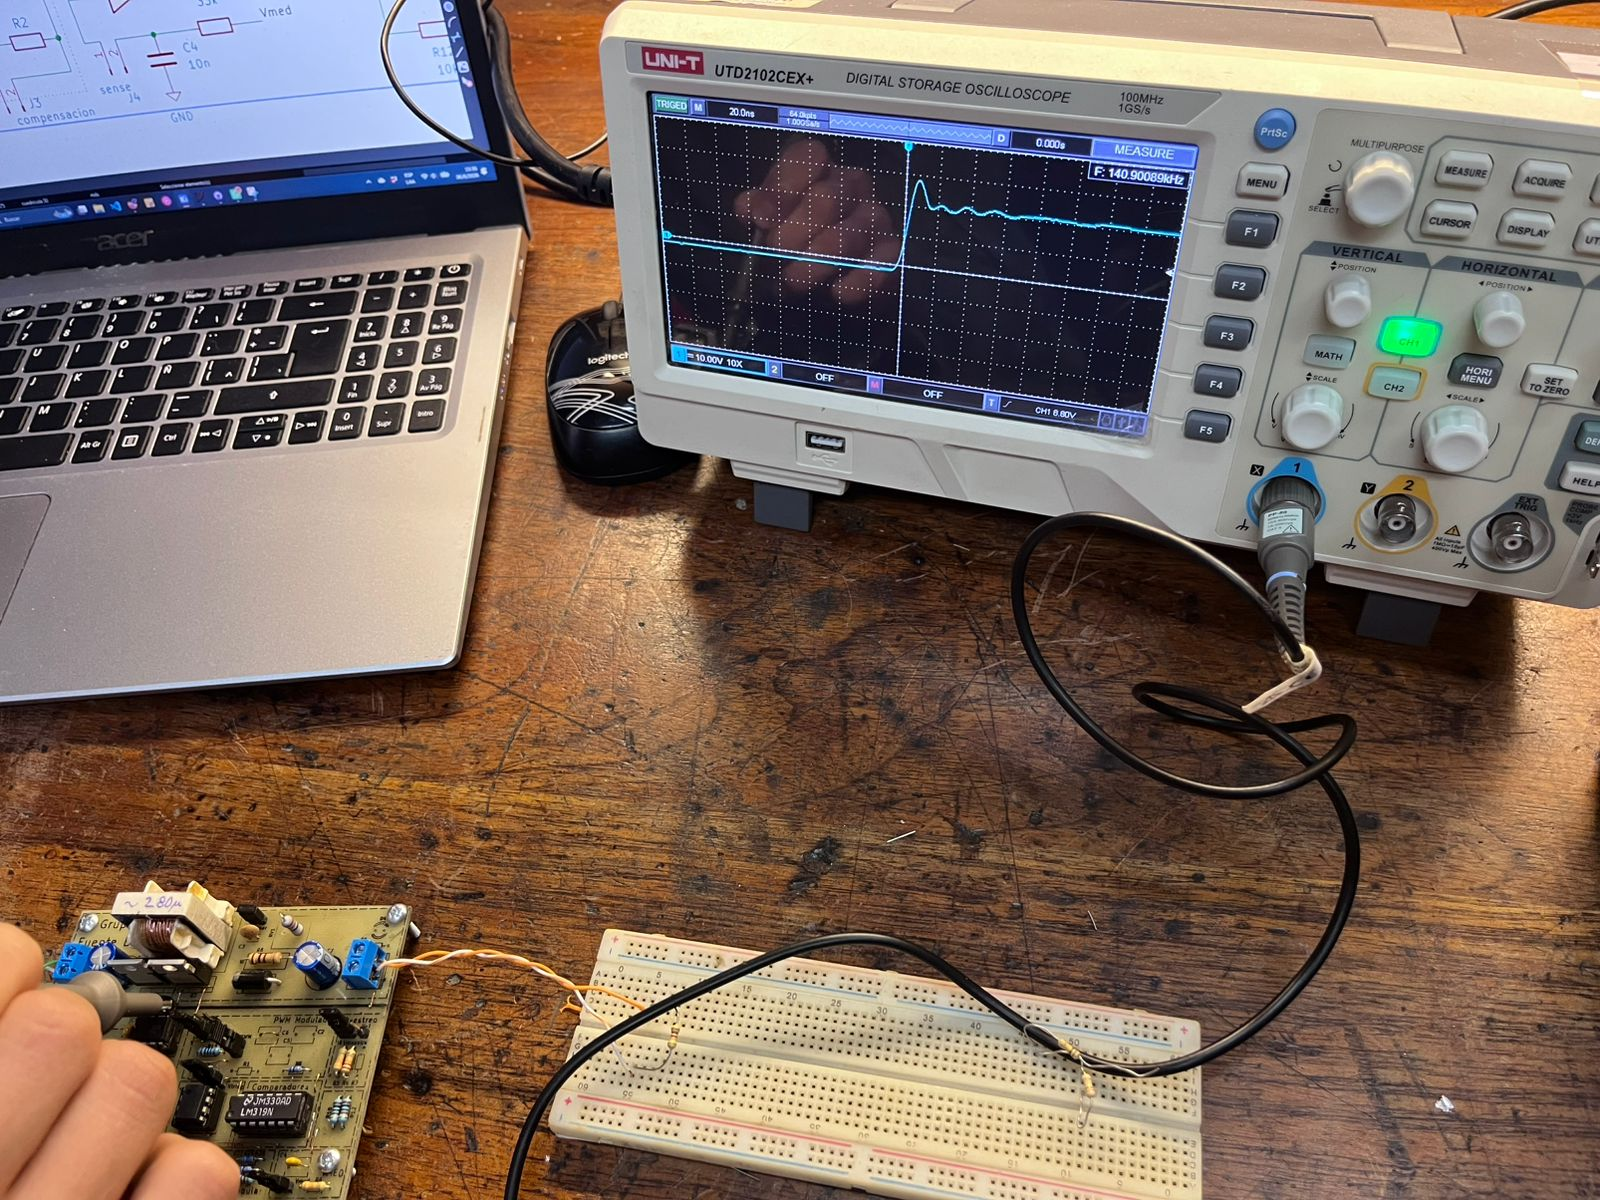
\includegraphics[width=\linewidth]{img/BUCK/medicion_con_snubber1}
			\caption{Medición con red \textit{Snubber}.}
			\label{fig:medicionconsnubber}
		\end{minipage}
		
	\end{figure}
	
	Notar que, si bien aun se puede apreciar un sobrepico, la señal se estabiliza mucho más rápido, asegurando la señal triangular de corriente en el bobinado.
	
	\subsubsection{Respuesta al encendido}
	
	Para esta prueba, se retira la red RC de \textit{slow-start} ($R_6$ , $C_4$ de la figura \ref{sec:apendice_PCB}), y se observa la respuesta temporal de la salida respecto de un impulso de entrada. La figura \ref{fig:encendido} muestra el resultado.
	
	\begin{figure}
		\centering
		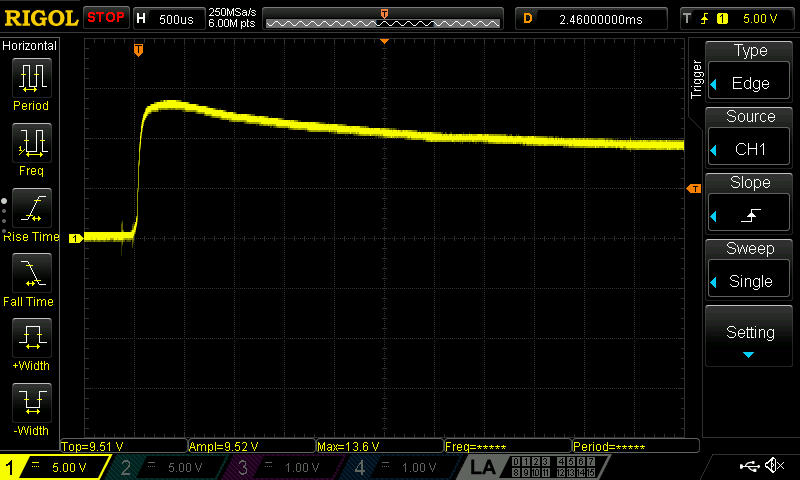
\includegraphics[width=0.7\linewidth]{img/BUCK/impulso}
		\caption{Respuesta al impulso de entrada.}
		\label{fig:encendido}
	\end{figure}
	
	Se observa que, si bien la forma de onda no es la misma a la esperada de las simulaciones (figura \ref{fig:sim_compensado}), el sistema se encuentra correctamente compensado. El tiempo de arranque también es considerablemente diferente, rondando los \SI{4}{ms}. Esto sugiere un ancho de banda considerablemente inferior a los resultados simulados. Si bien es un problema en cuanto a la efectividad de la fuente, no impide su correcto funcionamiento.
	
	
	\section{Errores}
	\subsection{Capacitor de suavizado de entrada}\hfill\break
	
	Se agrega un capacitor electrolítico de valor \SI{10}{\micro F} para suavizar la señal de entrada. Esto permite al circuito tomar corriente de forma abrupta, y minimiza el ruido de entrada a la salida del regulador.
	
	\subsection{Rango de regulación}\hfill\break
	
	Las mediciones reflejan un rango de entrada $\SI{5.3}{V} < V_{in} < \SI{16.5}{V}$ para el cuál la salida $V_o \approx \SI{5}{V}$.
	Una hipótesis, basada en la experiencia de diseño, es que la llave analógica satura cuando la tensión del lazo de corriente es muy pequeña. Una forma de evitar este fenómeno es reduciendo la resistencia $R_{16}$ y aumentando $R_{17}$ (figura \ref{fig:esquematicokicadldo}). Esto reduce la corriente por la rama central y, reduce la caída sobre $R_{16}$, mejorando el rango de $V_{ctrl}$, y en consecuencia el rango de regulación.
	\subsection{LDO}
	
	\subsection{BUCK}
	\subsubsection{Driver Defectuoso}
	Uno de los problemas más serios encontrados durante la implementación fue el funcionamiento anómalo del driver \textbf{IR2111}. La polarización del transistor $Q_2$ se vio anulada completamente.
	
	Adicionalmente, la entrada de control del driver, idealmente de alta impedancia, parecía cargar al circuito generador de PWM, deformando la señal, y retrasando la activación de los flancos ascendentes. Para solucionar esto, debió colocarse una resistencia de \textit{pull-up} anormalmente chica.
	
	\textit{Nota:} El origen de la falla es, con gran probabilidad, producto de una manupulación poco cuidadosa durante la etapa de testeo inicial del equipo. Es posible que alguna mala conexión involuntaria haya destruido parte del integrado. 
	
	\subsubsection{Ruido de conmutación} \label{sec:ruido}
	Se observó durante los experimentos que, a mayor tensión de entrada, más se inestabilizaba la fuente, pudiendo incluso dejar de regular.
	
	Investigando las señales del circuito, se encontró que la señal triangular se ve afectada por el ruido de conmutación de la fuente, haciendo que el comparador del circuito PWM accione antes de tiempo, y deforme la señal triangular de forma dramática (figura \ref{fig:ruido}).
	
	Sin la señal triangular como corazón del sistema, el lazo comienza a generar señales PWM fuertemente oscilantes, anulando el control sobre la salida.
	
	Debe analizarse el PCB con detenimiento para encontrar algún punto conflictivo, o en su defecto colocar un capacitor de filtrado que anule estos impulsos indeseados.
	
	Este problema acarrea otra consecuencia: el sistema deja de regular para cargas pequeñas. Por este motivo, fue imposible conseguir mediciones de eficiencia aceptables.
	
	Este problema puede ser resuelto de forma provisoria colocando un capacitor en el nodo de salida de la triangular, que sirve de suavizador, o aumentando el valor de capacidad de la red \textit{Snubber}, permitiendo realizar \textbf{mediciones parciales}.
	
	\begin{figure}[H]
		\centering
		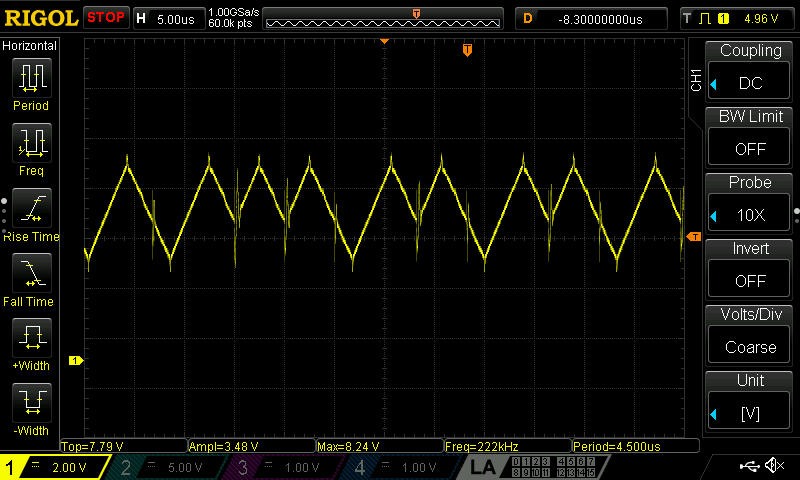
\includegraphics[width=0.7\linewidth]{img/BUCK/ruido}
		\caption{Medición de la señal triangular generada.}
		\label{fig:ruido}
	\end{figure}
	\begin{figure}[H]
		\centering
		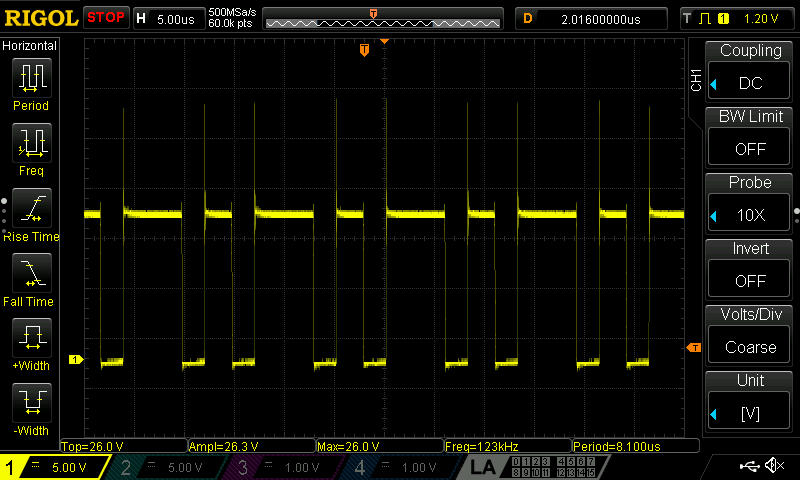
\includegraphics[width=0.7\linewidth]{img/BUCK/pwm}
		\caption{Medición del nodo $V_s$. Notar la señal PWM de duty irregular.}
		\label{fig:pwm}
	\end{figure}
	
	
\section{Conclusiones}

\subsection{Regulador Lineal LDO}

El regulador lineal diseñado cumple con las especificaciones de la tabla \ref{tabla:especificaciones_ldo}, sin embargo, no es ideal:

\begin{itemize}
	\item El rechazo de ripple de la fuente de alimentación no es bueno, y prácticamente permite el paso de toda la oscilación de entrada. Este punto debe ser analizado con mayor detalle al realizar la compensación del circuito.
	\item El lazo de corriente es lento, ya que cuenta con muchas etapas.
\end{itemize}

Asimismo, cuenta con algunas virtudes:
\begin{itemize}
	\item La regulación de línea es excelente, así como la regulación de carga.
	\item La eficiencia es muy buena para tratarse de un regulador lineal, sobre todo para resistencias de carga bajas.
	\item El valor de $V_{DO}$ es muy bueno.
\end{itemize}

Se concluye que el regulador es apto para la aplicación en este proyecto, pero se deberán tener precauciones durante el diseño de la etapa switching, o en su defecto se deberá robustecer el diseño.

Algunas reflexiones adicionales:
\begin{itemize}
    \item El limitador de corriente shunt actúa mas "rápido" que el limitador por foldback hecho con amplificadores operacionales, ya que estos últimos suelen ser "lentos".Esto permite que ante un corto (RL muy baja), no se dispare una elevada corriente y actúe primero el limitador de corriente.
    \item Un transistor de paso hecho con un PMOS presenta una tensión de Drop Out baja, este tipo de circuitos se los conoce como ''Low Drop Out''.
    \item Utilizar cargas activas en los amplificadores diferenciales presentan una mejor RRMC.
\end{itemize}

\subsection{Regulador BUCK}

El regulador funciona correctamente tras ciertas adaptaciones provisorias, que permiten anular una parte del ruido de conmutación que se filtra el circuito PWM.

Los resultados respetaron, en su mayoría, los requerimientos pedidos, a excepción de algunos valores particualres, como la eficiencia. Si bien se podría aspirar a valores cercanos al 95\%, no son malos para un primer prototipo.

La fuente podría usar algunas mejoras, como protecciones a la carga y a la alimentación, y para sí misma. Además, se requiere un estudio de propagación de ruido de conmutación, que fue lo que ocasionó graves problemas durante el desarrollo, e incluso tras las correcciones, sigue volviendo a la fuente inestable bajo ciertos escenarios.

Asimismo, si bien la compensación demuestra ser robusta en las simulaciones, se podría evaluar la posibilidad de aumentar el margen de fase a costa de ancho de banda, y de esta forma asegurar aún más la estabilidad.

Por otro lado, la elección del filtro \textit{Snubber} resultó ser insuficiente: no llega a amortiguar del todo los sobrepicos de tensión sobre el nodo de conmutación. Para corregir esto, bastará con elegir una capacidad más grande a costa de menor eficiencia (pero mayor robustez y estabilidad a la salida).

La eficiencia podrá ser mejorada fácilmente con el refinamiento del circuito de conmutación. En particular, la resistencia de \textit{pull-up} responsable de alimentar al gate driver, consume casi \SI{25}{mA} en estado bajo. También se puede jugar con la corriente de alimentación de los reguladores lineas, entre otras cosas, acercándonos a la combinación de valores más eficiente.


	{\footnotesize
		\printbibliography
	}
	
	
	\appendix
	\begin{landscape}
	\section{Apéndice I: Simulaciones}
	\label{sec:apendice_simulaciónes}
	
	\subsection{LDO}
	
	\begin{figure}[H]
		\centering
		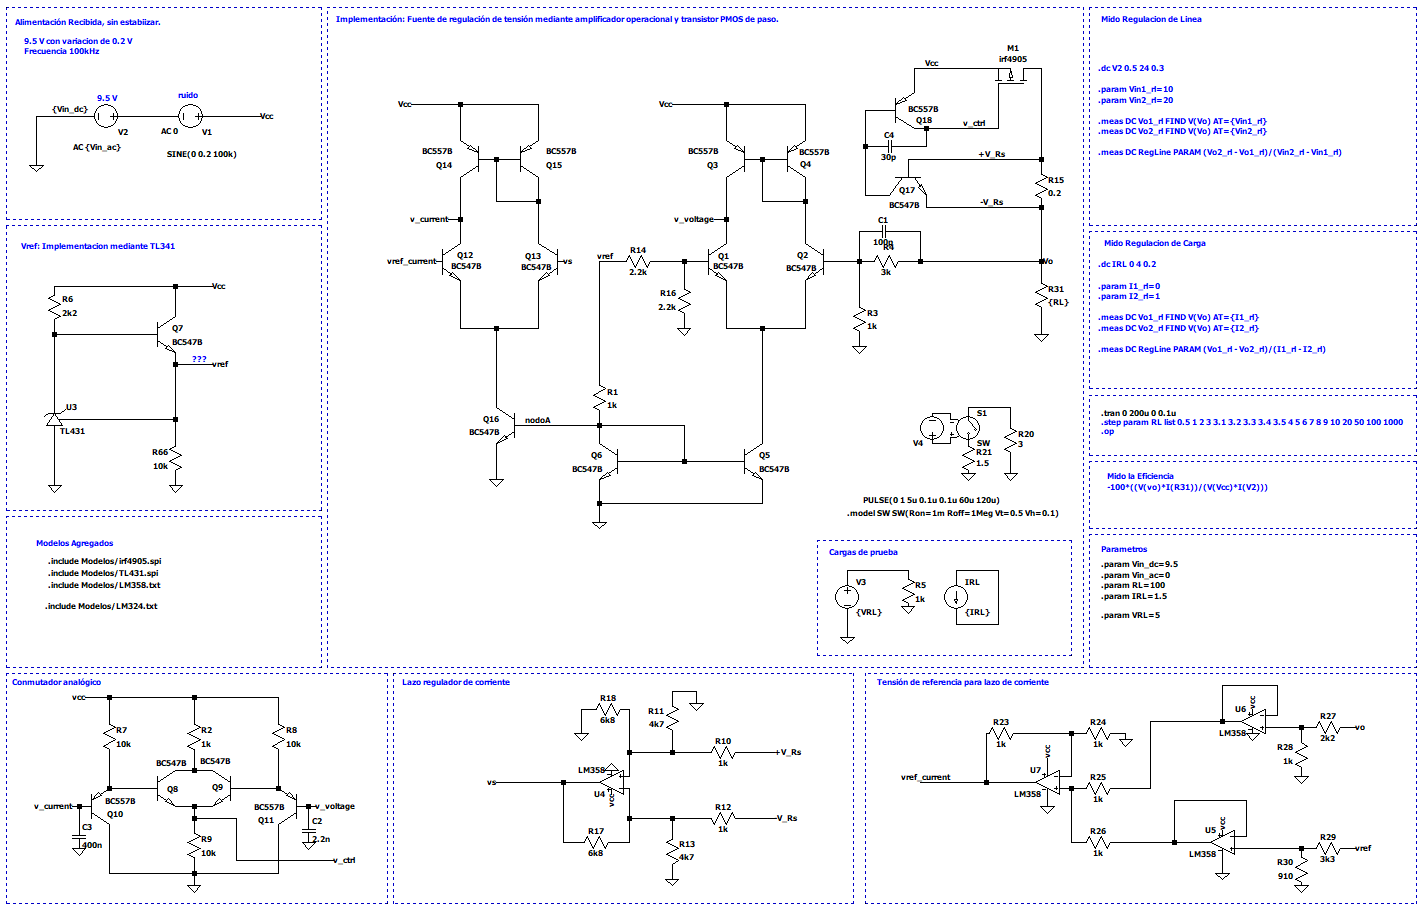
\includegraphics[width=0.85\linewidth]{img/LDO/Esquematico_LDO_LTSPICE2}
		\caption{Captura de simulación en LtSpice.}
		\label{fig:esquematicoldoltspice}
	\end{figure}
	
	\subsection{BUCK}
	\begin{figure}[H]
		\centering
		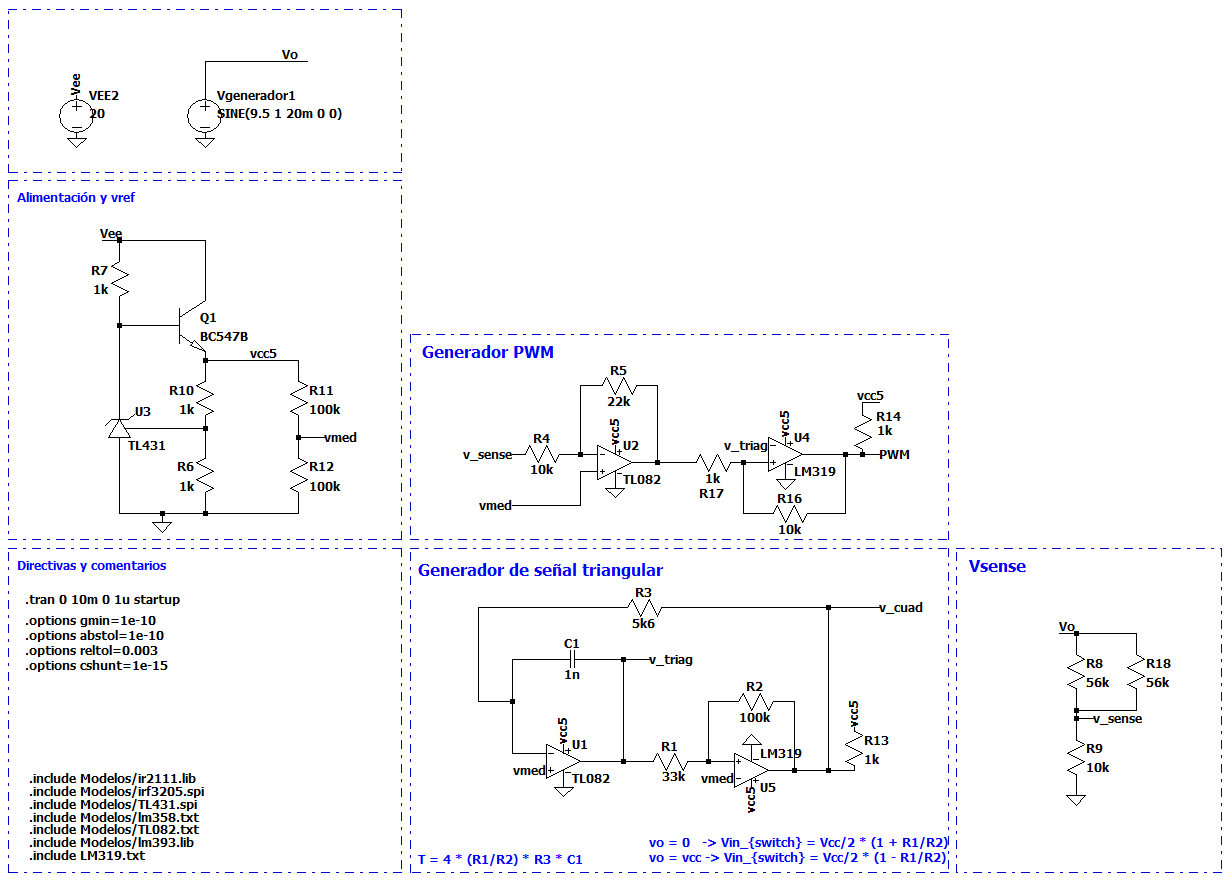
\includegraphics[width=0.85\linewidth]{img/BUCK/simulacion_pwm}
		\caption{Captura de simulación en LtSpice.}
		\label{fig:esquematicobuckpwm}
	\end{figure}
	\begin{figure}[H]
		\centering
		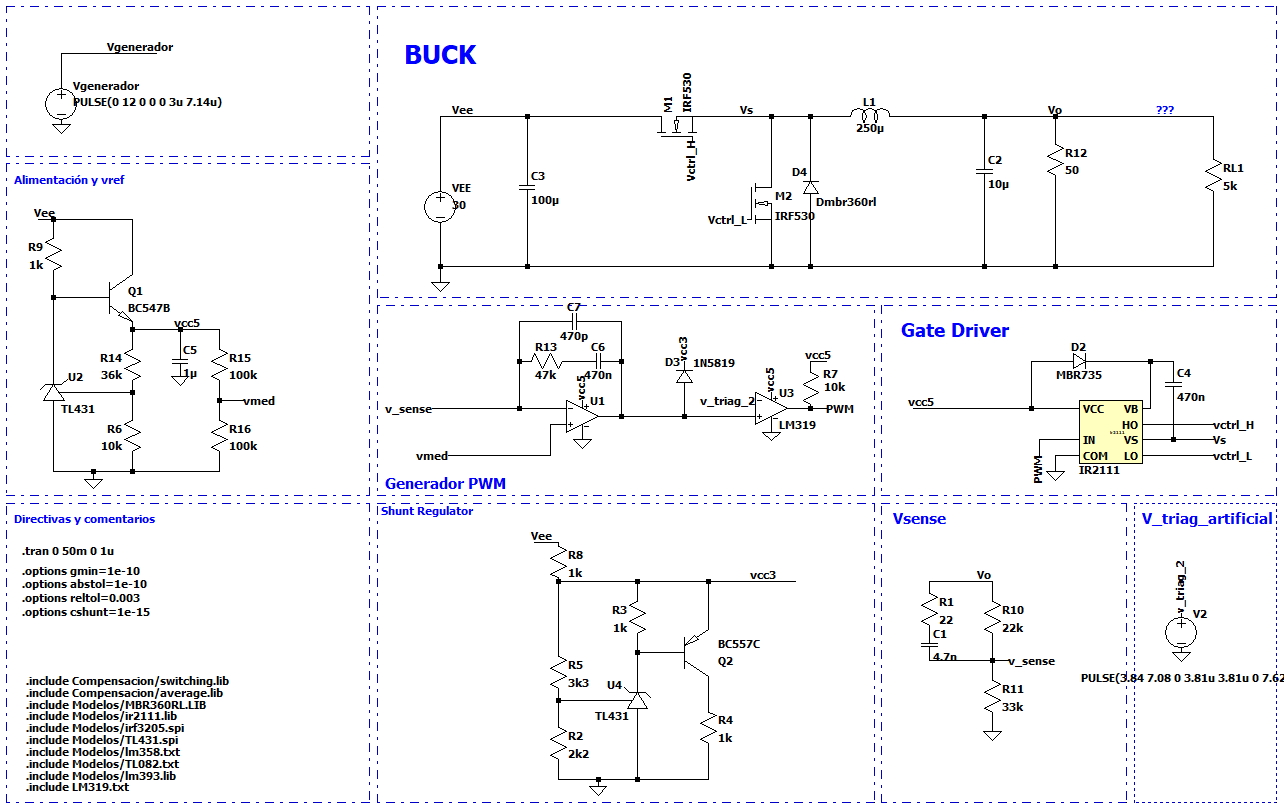
\includegraphics[width=0.85\linewidth]{img/BUCK/simulacion_buck}
		\caption{Captura de simulación en LtSpice.}
		\label{fig:esquematicobuck}
	\end{figure}
		\begin{figure}[H]
		\centering
		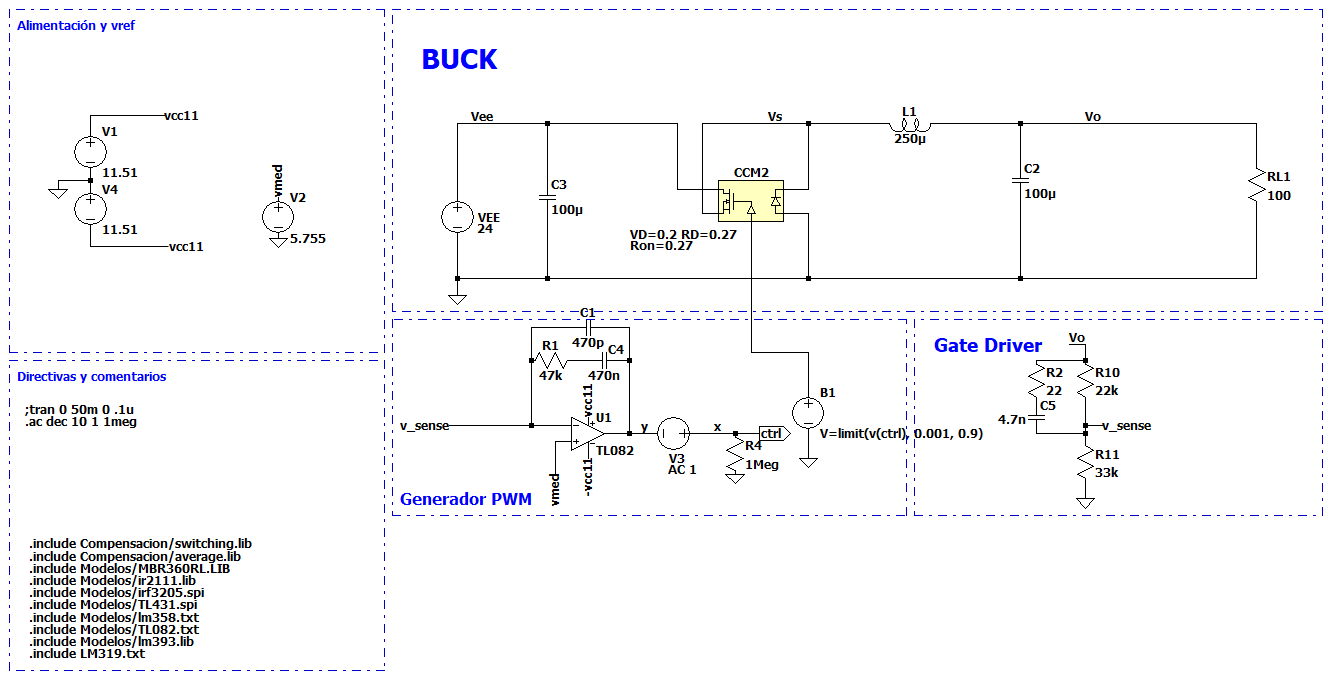
\includegraphics[width=0.85\linewidth]{img/BUCK/simulacion_buck_compensado}
		\caption{Captura de simulación en LtSpice.}
		\label{fig:esquematicobuckcompensado}
	\end{figure}
	

	\section{Apéndice II: Esquemáticos}
	\label{sec:apendice_esquematicos}
		
	\subsection{LDO}
	\begin{figure}[H]
		\centering
		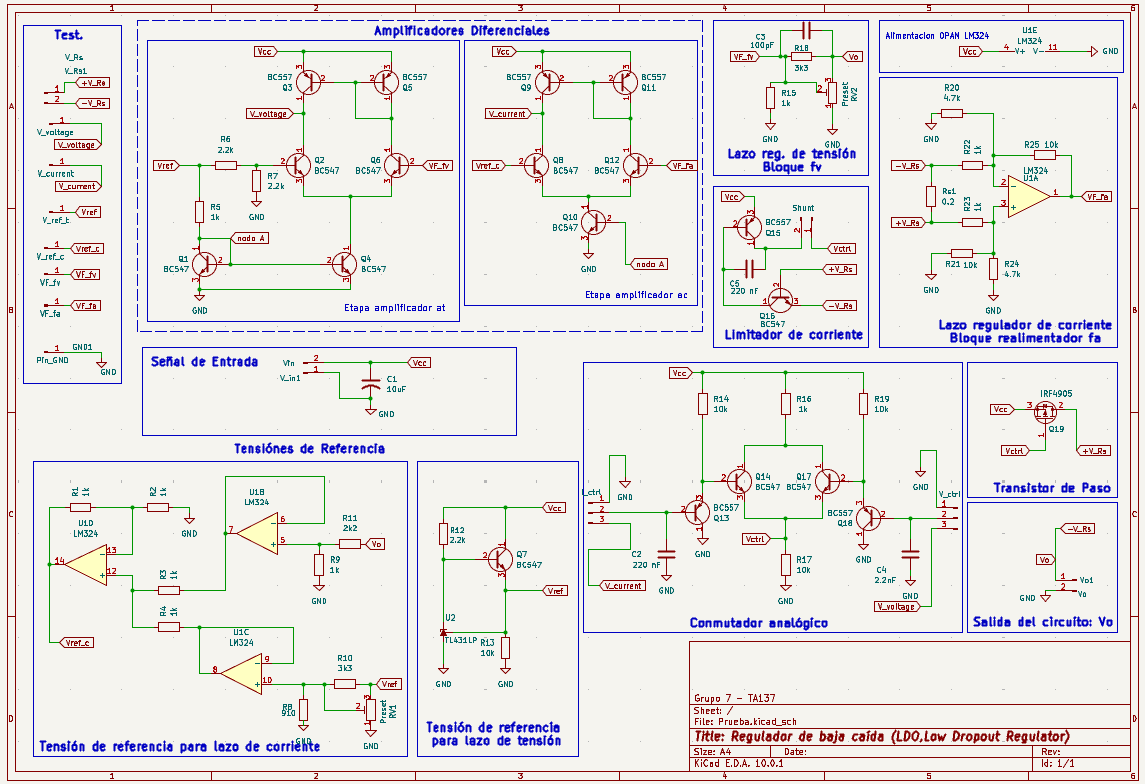
\includegraphics[width=0.85\linewidth]{img/LDO/esquematico_kicad_LDO}
		\caption{Esquemático de la implementación del regulador lineal LDO.}
		\label{fig:esquematicokicadldo}
	\end{figure}
	
	\subsection{BUCK}
		\begin{figure}[H]
		\centering
		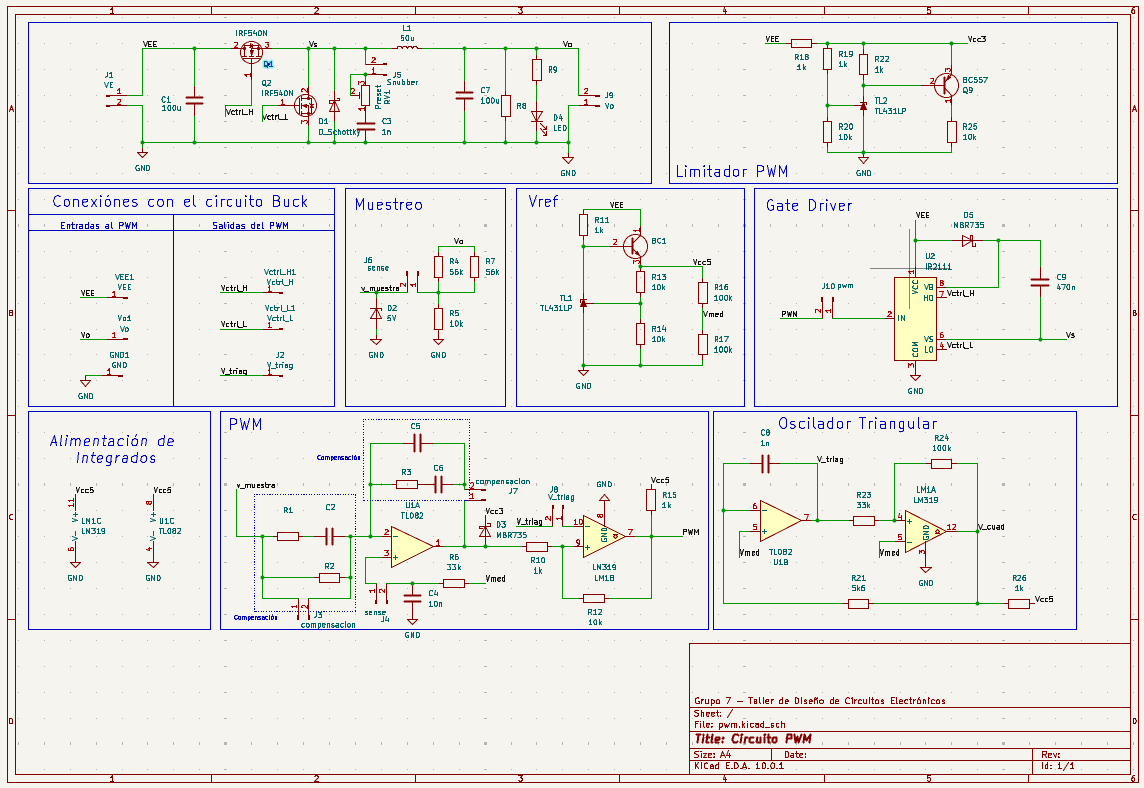
\includegraphics[width=0.85\linewidth]{img/BUCK/esquematico_buck}
		\caption{Esquemático de la implementación de la fuente switching tipo \textit{Buck}.}
		\label{fig:esquematicokicadbuck}
	\end{figure}
	
	\end{landscape}
\section{Apéndice III: PCB}
\subsection{LDO}
\label{sec:apendice_PCB}

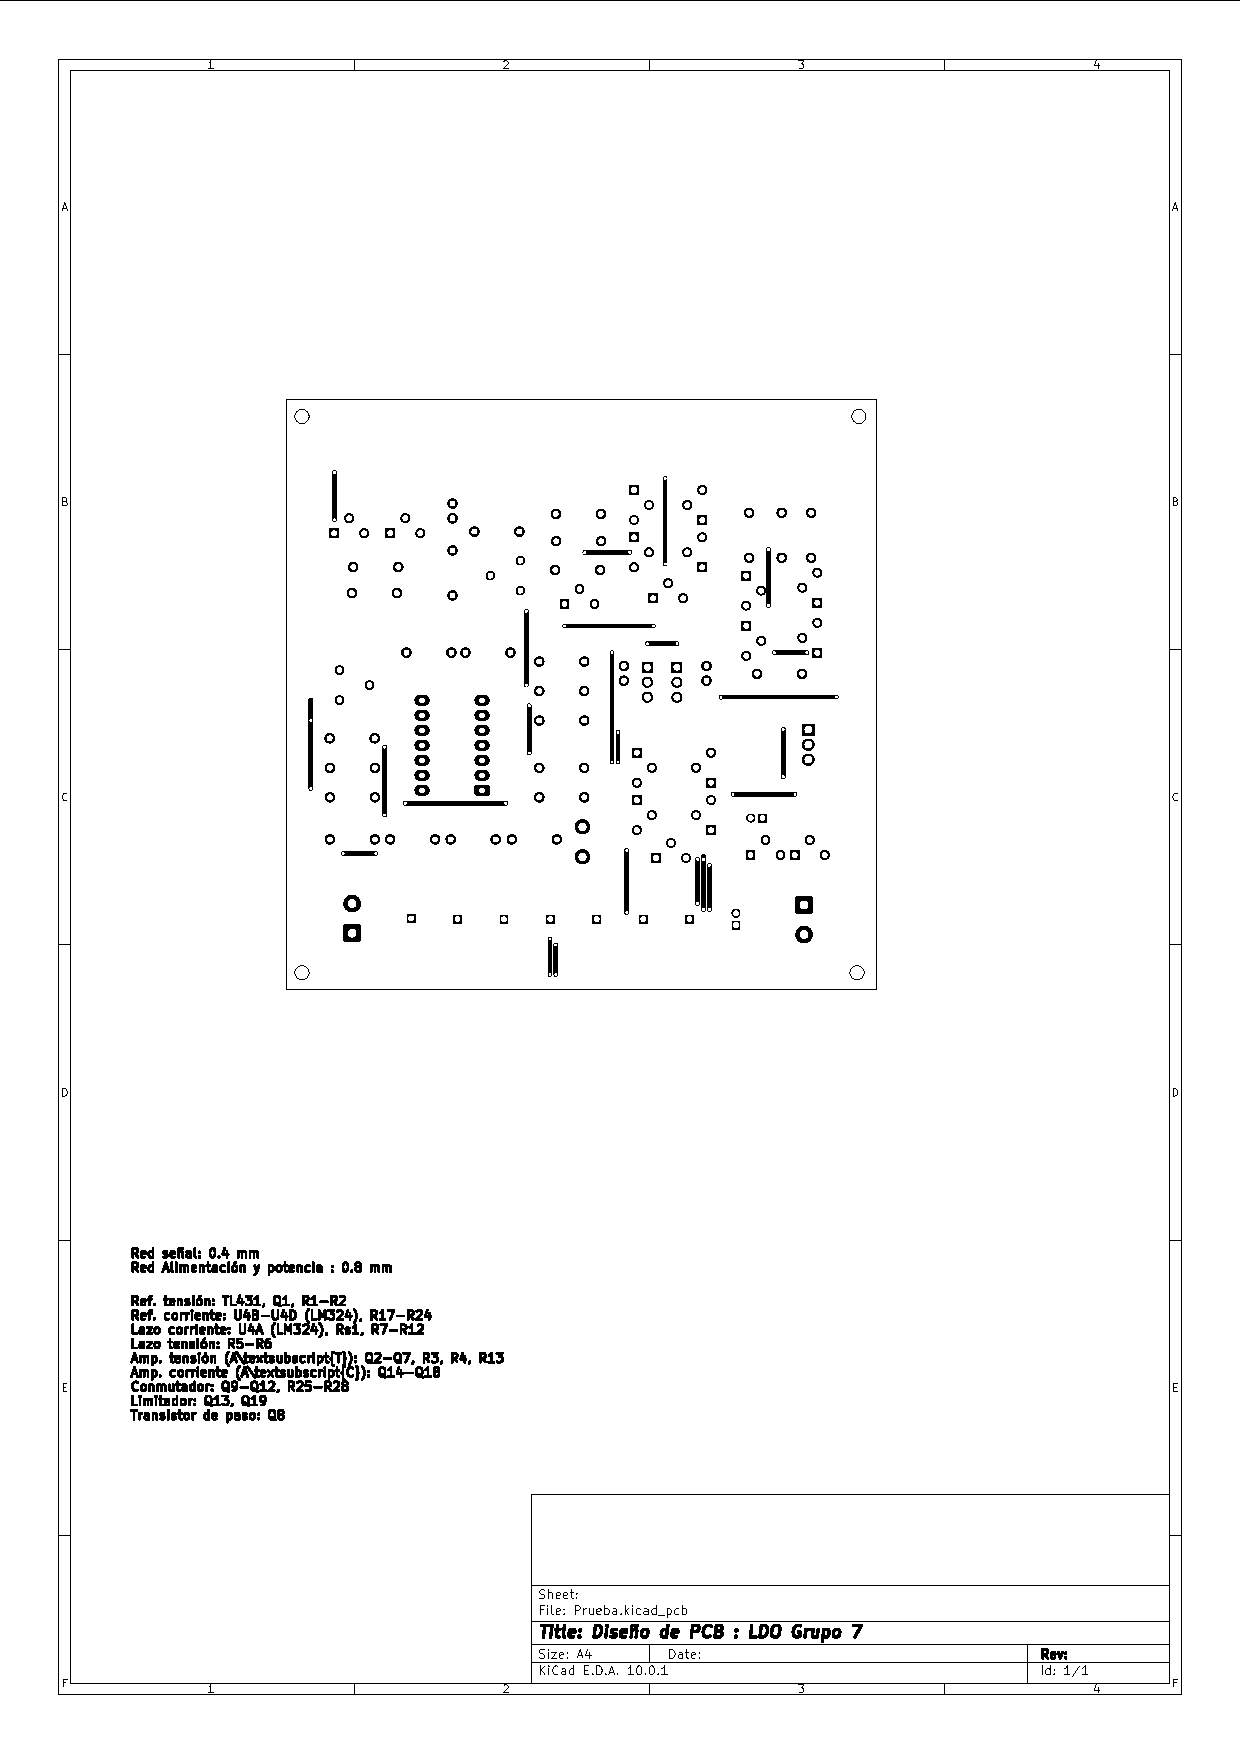
\includepdf[
pages=1,
pagecommand={
	\subsection{LDO capa superior}
}
]{img/LDO/pistas_LDO.pdf}

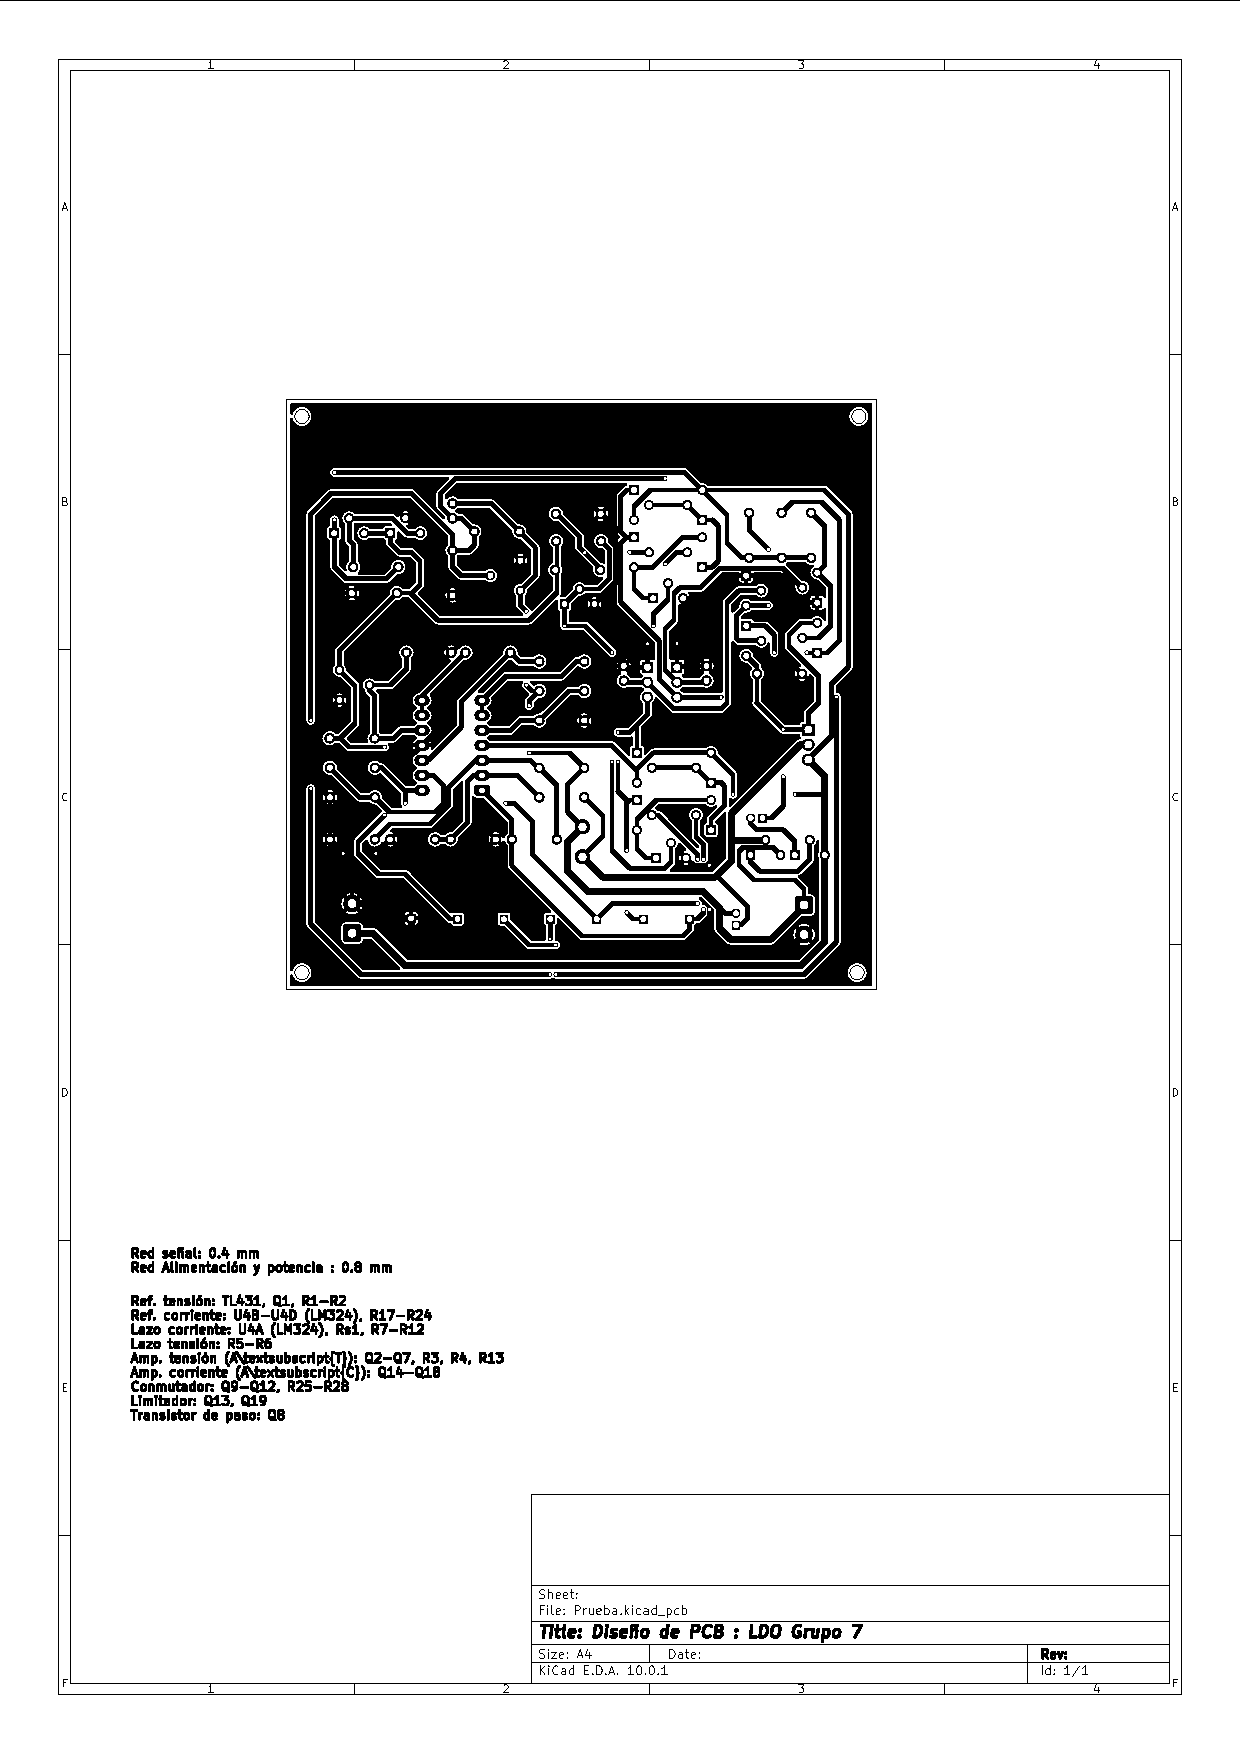
\includepdf[
pages=1,
pagecommand={
	\subsection{LDO capa inferior}
}
]{img/LDO/pistas_LDO_inferior.pdf}

\subsection{BUCK}
	
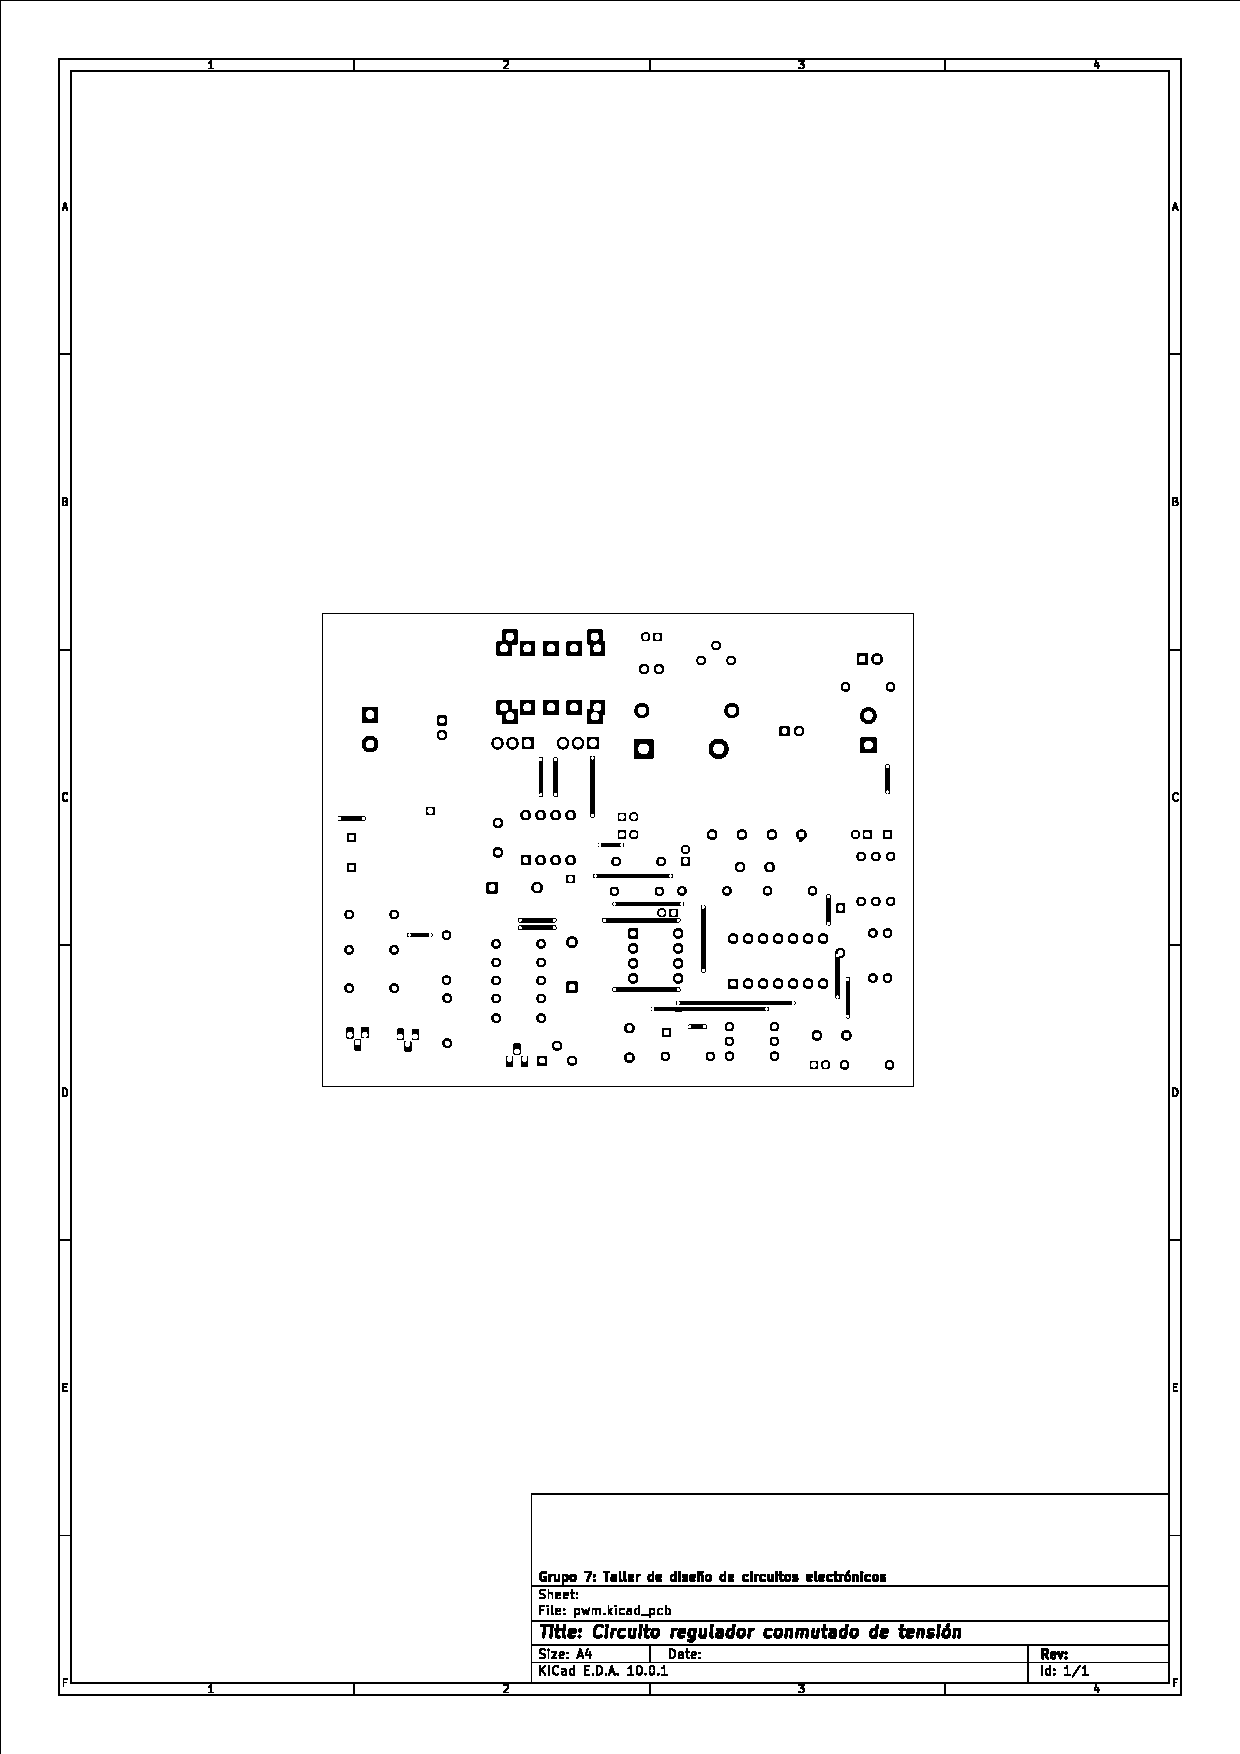
\includepdf[
pages=1,
pagecommand={
	\subsection{BUCK capa superior}
}
]{img/BUCK/pistas_BUCK.pdf}

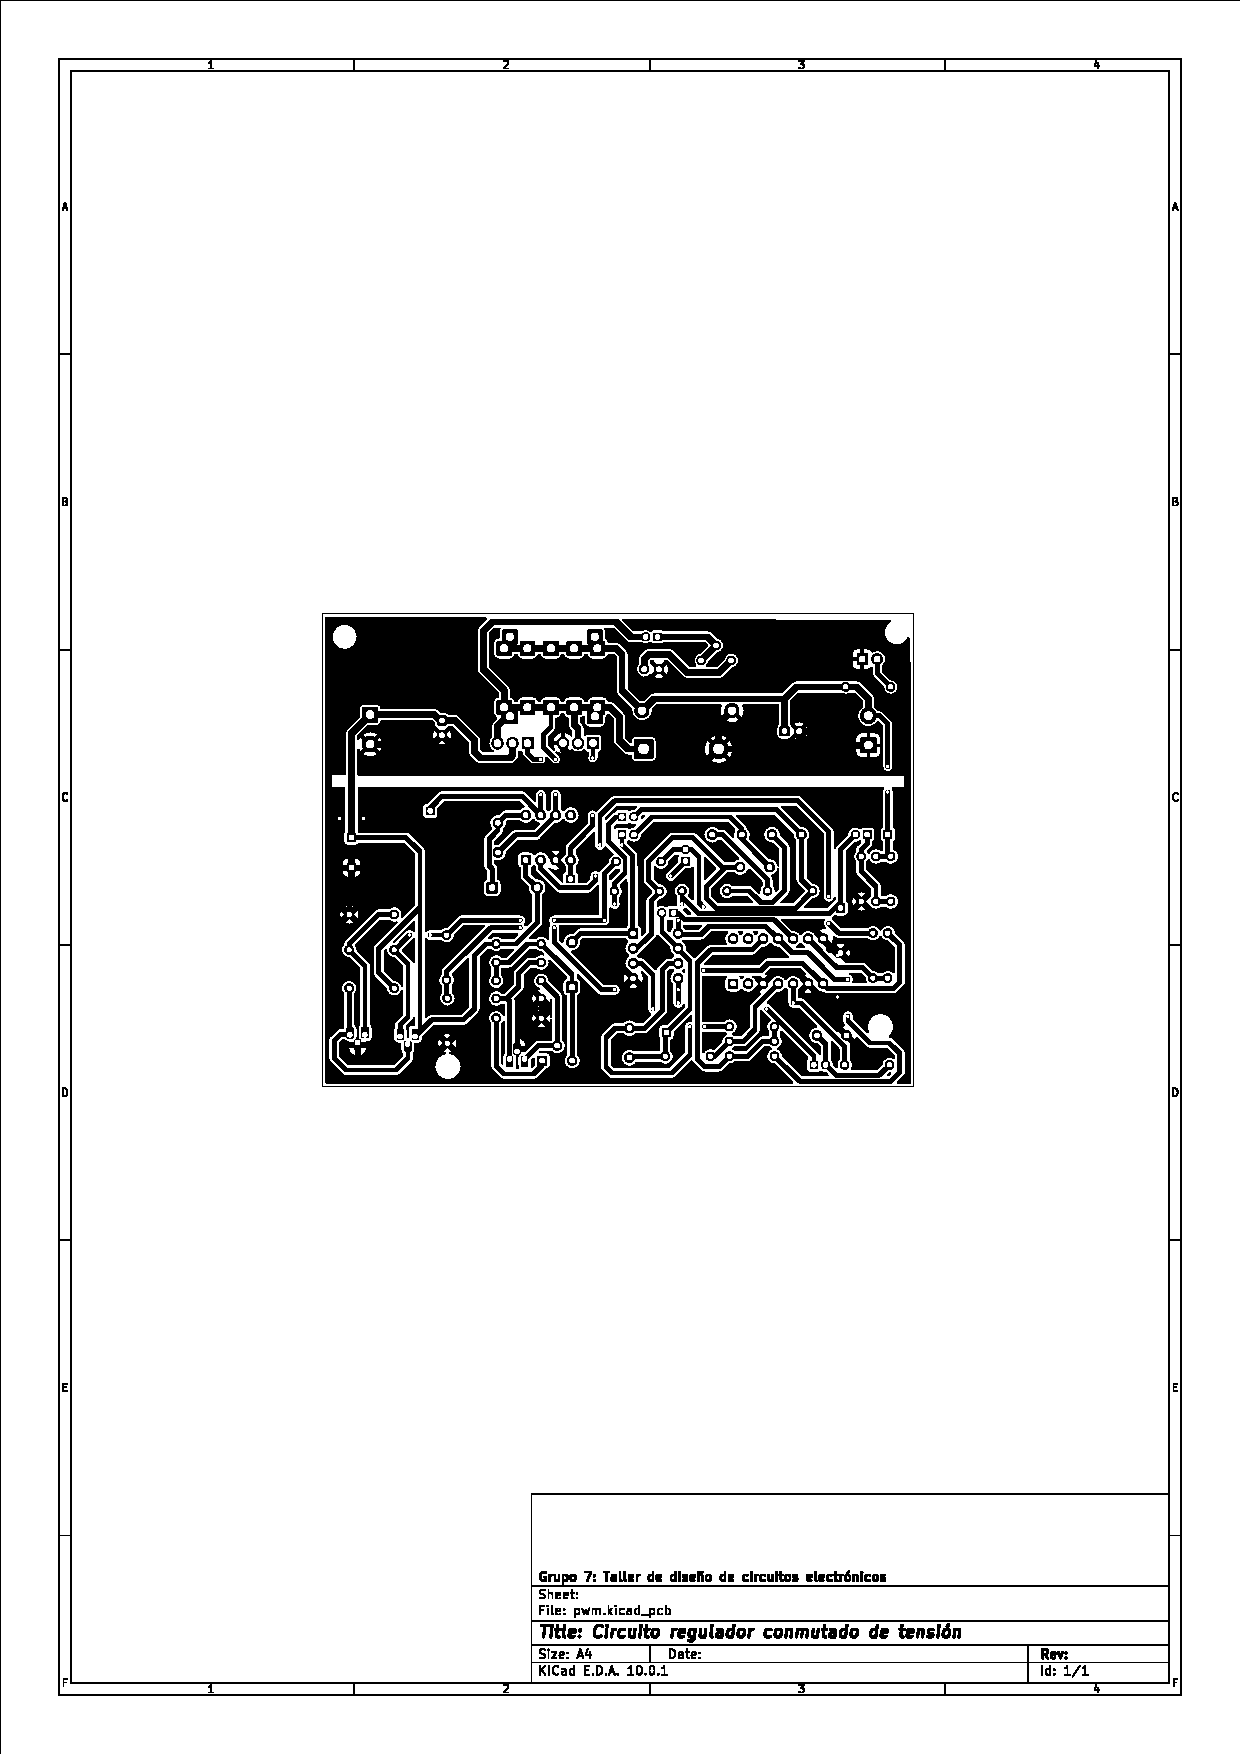
\includepdf[
pages=1,
pagecommand={
	\subsection{BUCK capa inferior}
}
]{img/BUCK/pistas_BUCK_inferior.pdf}
	
	
\end{document}
